% !TeX root = ../Book3.tex
% 纲要标题：# 第六编　非线性方法、几何流与奇异极限
% 纲要位置：几何学计划纲要.md，第 3120 行。
% 正文状态：本编导读初稿；尚未正式审核。

% 纲要内容开始
% 
% 纲要内容结束

\BookPart{非线性方法、几何流与奇异极限}{g3:part:06}
\BookPartGuide
几何方程中的尺度与对称性，使一般的存在性方法遇到新的困难。临界能量可以集中，微分同胚不变性可以造成主符号退化，光滑演化也可以在有限时间形成奇点。本编围绕这些具体障碍，研究规范固定、先验估计、重缩放及弱极限的方法。

\ProseParagraphBreak
\chapref{g3:ch:24}研究共形类中的 Yamabe 问题，从共形变化公式进入临界变分，分别处理非正情形和正情形的集中。\chapref{g3:ch:25}把 Einstein 方程视为度量上的非线性方程，说明规范怎样恢复椭圆性，无穷小形变与有限维障碍又怎样进入局部模问题。两章共同使用第三编的椭圆与非线性工具，但对未知量、约束和归一化作不同选择。

\ProseParagraphBreak
\chapref{g3:ch:26}建立所需的线性与拟线性抛物方法，并用调和映射热流展开短时、先验控制及调和代表的极限构造。\chapref{g3:ch:27}研究 Ricci 流，通过 DeTurck 规范恢复抛物性，再计算曲率演化、保持性质、孤立子与放大模型。\chapref{g3:ch:28}转向平均曲率流，推导光滑演化和 Huisken 单调公式，并区分水平集与 Brakke 等弱演化对象。

\ProseParagraphBreak
\chapref{g3:ch:29}从变化的几何空间本身研究极限。光滑紧性、塌缩和 Ricci 下界各自保留不同的结构，合成曲率与弱微分则提供无光滑坐标时的描述。这里与第二编的度量极限、第三编的能量以及第五编的弱对象重新相遇。

\ProseParagraphBreak
本编各章均可按问题选读。第24—25章需要第11—14章的椭圆和非线性分析；第26章接续调和映射变分，随后为 Ricci 流及平均曲率流提供抛物工具。第29章需要第10章的度量收敛，并按专题使用比较几何和弱能量。一般手术、深层非塌缩、弱演化全局存在及极限结构定理的版本在实际调用处注明；显式解、尺度计算和已展开的证明为理解这些输入提供具体准备。

% !TeX root = ../../Book3.tex
% 纲要标题：## 第24章*　Yamabe 问题与临界变分
% 纲要位置：几何学计划纲要.md，第 3122 行。
% 正文状态：初稿；尚未正式审核。

% 纲要内容开始
% 
% > 本章目标与证明范围：以共形标量曲率为贯穿问题，完整处理非正 Yamabe 情形及严格低于球面阈值时的紧性论证。正质量等完成一般正情形所需的深层输入明确外引，不把全部存在性挤进“典型结果”。
% 
% 纲要内容结束

\OptionalChapter{Yamabe 问题与临界变分}{g3:ch:24}
\BookChapterNumber{g3:ch:24}

\begin{chapterabstract}
	固定一个共形类，能否选出标量曲率为常数的度量？本章把这个问题写成带体积约束的临界变分问题，计算共形 Laplace 算子的协变公式与 Yamabe 泛函的一、二阶变分。非负弱极小点通过截断吸收、椭圆正则性和最大值原理恢复为光滑正因子。对于非正 Yamabe 常数，直接方法给出存在性，并证明固定体积后的唯一性；对于严格低于球面常数的情形，用近锐 Sobolev 不等式、范数分裂和能量缺陷估计完整证明极小化序列的强紧性。最后说明局部曲率、Green 函数和正质量如何提供严格不等式，准确引用一般存在性所需的深层结果，并以谱与球面模型辨别临界点、局部极小和全局极小。
\end{chapterabstract}

\begin{learninggoals}
	\begin{itemize}
		\item 在非负 Laplace 约定下计算共形标量曲率、体积与共形能量的变化。
		\item 区分 \(H^1\) 能量空间、高正则性空间中的正开集与单位体积约束，验证变分的可微性。
		\item 由第一特征函数识别共形类的符号，并完整证明临界非负弱解的光滑正性。
		\item 对负值和零值分别证明极小化序列紧性，建立非正情形的存在与规范体积唯一性。
		\item 计算临界气泡的尺度、低阶范数与球面能量，解释端点 Sobolev 嵌入失紧。
		\item 证明范数分裂、近锐 Sobolev 估计及严格球面阈值下的极小值实现。
		\item 说明 Aubin 型局部测试与 Schoen 的 Green 函数方法各解决哪些情形，核对所用正质量版本。
		\item 计算约束 Hessian，并用球面共形变化及长圆柱乘积区分存在性、稳定性与唯一性。
	\end{itemize}
\end{learninggoals}

在曲面上，标量曲率是 Gauss 曲率的两倍；在高维，标量曲率只是所有截面曲率的一项收缩。固定共形类后要求它为常数，是一个未知正函数满足的一条标量方程。这个问题称为\term[Yamabe wenti]{Yamabe 问题}[Yamabe problem]。\footnote{\OriginalHanName{山辺英彦}（やまべ ひでひこ，Hidehiko Yamabe，1923--1960），日本数学家，研究拓扑群与微分几何。}它不要求各个截面方向的曲率相等，因而比常截面曲率条件保留了更多几何自由。

\ProseParagraphBreak
第3章的共形变化公式把曲率条件化成非线性椭圆方程。第三编已经提供 Sobolev 空间、椭圆正则性、Banach 微分与约束变分，眼下的新障碍是临界指数：一列共形因子可以在越来越小的区域变得越来越高，保持总体积，却在弱极限中消失。局部的 Euclid 气泡显示了这种集中所需的确切能量；它恰等于圆球的 Yamabe 常数。

\ProseParagraphBreak
本章先从能量符号入手。非正情形不需要锐常数就能恢复强收敛，并可用最大值原理比较两个正解。随后把一般极小化序列分成弱极限与余项，证明只要极小值严格低于球面常数，任何质量损失都会违反极小性。最后，Aubin\footnote{Thierry Émilien Flavien Aubin（1942--2009），法国数学家，研究黎曼几何与非线性偏微分方程。}的局部测试和 Schoen 的整体构造负责取得这个严格不等号；正质量输入连同其维数、共形平坦及刚性条件在第24.5节列出。共形方程、球面模型与变分方法的原文组织可参看\cite[第2--4节]{LeeParker1987Yamabe}。

% !TeX root = ../../Book3.tex
% 纲要标题：### 24.1 Yamabe 问题的变分设置
% 纲要位置：几何学计划纲要.md，第 3126 行。
% 正文状态：初稿；尚未正式审核。

% 纲要内容开始
% 
% 本章不再首次建立通用非线性工具；它们的证明位置统一前移至第三编。
% 
% * 函数空间与变分方法
% * 固定共形类、正因子及体积约束
% * 弱极小点与光滑正解
% * 第一特征值、Yamabe 常数与唯一性
% 
% 纲要内容结束

\section{Yamabe 问题的变分设置}
\label{g3:sec:2401}

本章固定一个闭、连通、光滑的黎曼流形 \((M^n,g)\)，其中 \(n\ge3\)。闭表示紧且无边界；积分使用黎曼体积密度，所以不要求可定向。记
\[
	s_g=\operatorname{Scal}_g,\qquad
	a_n=\frac{4(n-1)}{n-2},\qquad p=\frac{2n}{n-2},\qquad
	\Delta_g=-\operatorname{div}_g\nabla.
\]
于是 \(\int_M v\Delta_gv\,\mu_g=\int_M|\mathrm dv|_g^2\,\mu_g\)。以下的曲率方程、极值比较与能量公式都使用这一非负 Laplace 约定。

\subsection{函数空间与变分方法}
\label{g3:subsec:2401:01}
第13.5节的 Banach 隐函数定理适合研究已知解附近的变化，第13.6节的复合与约束变分则负责把方程放进函数空间。本章先用能量寻找一个解，再在取得解后研究它的正则性与变分性质。这样做所需的空间有两种。

\ProseParagraphBreak
极小化采用实 Hilbert 空间 \(H^1(M)\)。由\cref{g3:thm:compact-bundle-sobolev,g3:thm:compact-bundle-rellich}，有
\[
	H^1(M)\longrightarrow L^p(M),\qquad
	H^1(M)\lhook\joinrel\longrightarrow L^q(M)\quad(1\le q<p),
\]
其中前一嵌入连续，后一嵌入紧。特别地，\(H^1\) 有界列能抽出在 \(L^2\) 中强收敛的子列，但单位 \(L^p\) 范数可能在弱极限中损失。这个端点差别正是临界变分的困难。

\ProseParagraphBreak
研究光滑正解的局部变化时，可选 \(r>n\) 并使用
\[
	\mathcal U_r=\{u\in W^{2,r}(M):\min_Mu>0\}.
\]
连续嵌入 \(W^{2,r}\to C^1\) 使它成为开集。由\cref{g3:thm:sobolev-composition-smooth}，在此集合上取实数幂、倒数及对数都是光滑的 Sobolev 复合。相应的曲率方程可作为到 \(L^r(M)\) 的光滑映射处理。\(H^1\) 中的非负锥则不是这样的开集：在一个小球中加入高度固定的负凸起，其 \(H^1\) 范数随球半径趋零，因为 \(n>2\)。因此不能把高正则性空间中的正开集直接搬到能量空间。

\subsection{固定共形类、正因子及体积约束}
\label{g3:subsec:2401:02}
\termidx[gongxing lei]{共形类}
\foreignidx{conformal class}
\begin{definition}\label{g3:def:yamabe-class-constraint}
	设 \((M^n,g)\) 为闭连通光滑黎曼流形，\(n\ge3\)。
	记 \(p=2n/(n-2)\)。
	\(g\) 的光滑共形类是
	\[
		[g]=\{u^{4/(n-2)}g:u\in C^\infty(M),\ u>0\}.
	\]
	对正因子 \(u\)，记 \(g_u=u^{4/(n-2)}g\)。体积变化为
	\[
		\mu_{g_u}=u^p\mu_g,\qquad
		\operatorname{Vol}(M,g_u)=\int_Mu^p\,\mu_g.
	\]
	在 \(H^1(M)\) 中相应采用约束 \(C(u)=\int_M|u|^p\,\mu_g=1\)。
\end{definition}
\symidx{\([g]\)：黎曼度量 \(g\) 的光滑共形类}

体积公式来自行列式：度量乘以 \(u^{4/(n-2)}\)，体积密度乘以它的 \(n/2\) 次方。每条正射线 \(\{tu:t>0\}\) 因而恰有一个单位体积代表 \(u/\|u\|_p\)。这只固定常数伸缩；对流形作共形自微分同胚仍可能产生不同的单位体积度量。

\begin{lemma}\label{g3:lem:yamabe-constraint-smoothness}
	设 \((M^n,g)\) 为闭连通光滑黎曼流形，\(n\ge3\)。
	记 \(p=2n/(n-2)\)。
	令 \(C(u)=\int_M|u|^p\,\mathrm d\mu_g\)，则 \(C:H^1(M)\to\mathbb R\) 为 \(C^2\) 映射，且
	\[
		\mathrm DC(u)h=p\int_M|u|^{p-2}uh\,\mu_g,\qquad
		\mathrm D^2C(u)[h,k]=p(p-1)\int_M|u|^{p-2}hk\,\mu_g.
	\]
	在 \(C(u)=1\) 处，其微分满射，约束切空间为
	\(\{h:\int_M|u|^{p-2}uh\,\mu_g=0\}\)。
\end{lemma}
\begin{proof}
	由 Hölder 不等式，三个因子 \(|u|^{p-2},h,k\) 的指数分别为 \(p/(p-2),p,p\)，所以第二式定义连续双线性型。映射 \(u\mapsto |u|^{p-2}\) 从 \(L^p\) 连续到 \(L^{p/(p-2)}\)：当 \(p-2\le1\) 时用幂函数的 Hölder 估计，当 \(p-2>1\) 时用中值公式和 Hölder 不等式。沿线段积分这个连续双线性型，先得到一阶微分的余项估计，再得到 \(C\) 的微分公式，故确为 Fréchet 二次连续可微。连续嵌入 \(H^1\to L^p\) 将结论限制到 \(H^1\)。最后 \(\mathrm DC(u)u=p\ne0\)，故微分满射；第13.5节的水平集定理给出所述切空间。
\end{proof}

这里没有要求 \(C\) 在 \(H^1\) 上无限次可微。临界指数可能不是整数，而约束乘子和二变分只需上述可微性。

\subsection{弱极小点与光滑正解}
\label{g3:subsec:2401:03}
先写出后续使用的解析量：
\begin{equation}\label{g3:eq:yamabe-energy-definition}
	L_g=a_n\Delta_g+s_g,\qquad
	E_g(u)=\int_M(a_n|\mathrm du|_g^2+s_gu^2)\,\mu_g,\qquad
	Q_g(u)=\frac{E_g(u)}{\|u\|_p^2}\quad(u\ne0).
\end{equation}
\symidx{\(L_g\)：共形 Laplace 算子 \(\frac{4(n-1)}{n-2}\Delta_g+s_g\)}
\symidx{\(Q_g\)：Yamabe 商}
\(L_g\) 称为\term[gongxing Laplace suanzi]{共形 Laplace 算子}[conformal Laplacian]。下一节将由曲率变化证明：\(Q_g(u)\) 正是 \(g_u\) 的规范化总标量曲率。它对 \(u\) 的常数倍不变，因此可以在 \(C=1\) 上最小化 \(E_g\)。

\begin{definition}\label{g3:def:yamabe-constant}
	设 \((M^n,g)\) 为闭连通光滑黎曼流形，\(n\ge3\)。
	对所用度量 \(h\)，记 \(E_h(v)=\int_M(\tfrac{4(n-1)}{n-2}|\mathrm dv|_h^2+s_hv^2)\,\mathrm d\mu_h\)，\(Q_h(v)=E_h(v)/\|v\|_{L^{2n/(n-2)}(h)}^2\)（\(v\ne0\)）。
	固定共形类的\term[Yamabe changshu]{Yamabe 常数}[Yamabe constant]定义为
	\[
		Y(M,[g])=\inf_{0\ne u\in H^1(M)}Q_g(u).
	\]
	\symidx{\(Y(M,[g])\)：共形类 \([g]\) 的 Yamabe 常数}
	本章简称 \(Y\)。这个量只对给定共形类取下确界；对所有共形类再取上确界是另一个不变量。
\end{definition}

\begin{proposition}\label{g3:prop:yamabe-admissible-density}
	设 \((M^n,g)\) 为闭连通光滑黎曼流形，\(n\ge3\)。记 \(Y=Y(M,[g])\) 为 \([g]\) 的 Yamabe 常数。
	\(Y\) 有限，并且其定义中的竞争者可以依次限制为非负 \(H^1\) 函数、光滑正函数，所得下确界不变。
\end{proposition}
\begin{proof}
	令 \(s_g^- =\max\{-s_g,0\}\)，由有限体积上的 Hölder 不等式，
	\[
		E_g(u)\ge a_n\|\mathrm du\|_2^2-\|s_g^-\|_\infty
		\operatorname{Vol}(M,g)^{2/n}\|u\|_p^2.
	\]
	所以 \(Y> -\infty\)；用 \(u=1\) 作竞争者又得有限上界。Sobolev 链式法则给出 \(|u|\in H^1\) 以及 \(|\mathrm d|u||=|\mathrm du|\) 几乎处处成立，故 \(Q_g(|u|)=Q_g(u)\)。这个等式在零水平集上使用了弱导数在那里几乎处处为零的性质，已在第11章的截断论证中建立。

	光滑函数在 \(H^1\) 中稠密，连续嵌入又使 \(L^p\) 范数收敛，因而 \(Q_g\) 在非零 \(H^1\) 函数上连续。对每个光滑实函数 \(v\)，取 \(v_\varepsilon=(v^2+\varepsilon^2)^{1/2}>0\)。它在 \(H^1\) 中趋于 \(|v|\)：导数是 \(v\,\mathrm dv/(v^2+\varepsilon^2)^{1/2}\)，由支配收敛及零水平集性质得到导数收敛。依次作光滑逼近和这一正化，就得到所需光滑正竞争者。
\end{proof}

极小值若在非零 \(H^1\) 函数处取得，先取绝对值、再规范体积，便得到非负的单位极小点。\Cref{g3:prop:constraint-lagrange-banach}随后产生弱 Euler 方程。将这个弱解恢复成光滑正函数，还需处理临界幂的可积性；\cref{g3:thm:yamabe-weak-regularity}将用截断和吸收先提高可积指数，再调用第12—13章的椭圆自举。这样，弱极小值才真正对应共形类中的光滑度量。

\subsection{第一特征值、Yamabe 常数与唯一性}
\label{g3:subsec:2401:04}
零阶函数 \(s_g\) 可以变号。决定共形类符号的量是整个二次型，而不只是某一点的标量曲率。考虑它的最低 Rayleigh 商
\[
	\lambda_1(L_g)=\inf_{v\ne0}\frac{E_g(v)}{\|v\|_2^2}.
\]
\begin{proposition}\label{g3:prop:yamabe-first-eigenvalue-sign}
	设 \((M^n,g)\) 为闭连通光滑黎曼流形，\(n\ge3\)。共形 Laplace 算子取 \(L_g=\tfrac{4(n-1)}{n-2}\Delta_g+s_g\)，其中 \(\Delta_g=-\operatorname{div}_g\nabla\)。记 \(Y=Y(M,[g])\) 为 \([g]\) 的 Yamabe 常数。
	\(L_g\) 有光滑严格正的第一特征函数 \(\phi\)，其特征空间为一维。\(Y\) 与 \(\lambda_1(L_g)\) 同号。特别地，\(Y=0\) 时 \(\ker L_g=\mathbb R\phi\)；\(Y>0\) 时核为零。
\end{proposition}
\begin{proof}
	在 \(\|v\|_2=1\) 上取极小化序列。零阶项有下界，所以导数范数有界；Rellich 紧性保留 \(L^2\) 约束，导数范数弱下半连续，故下确界取得。取绝对值后可设极小点非负，约束变分给出 \(L_g\phi=\lambda_1\phi\)。光滑系数椭圆正则性逐次提高 Sobolev 阶数，得到 \(\phi\) 光滑。写成 \(\Delta_g\phi=V\phi\)，其中 \(V=(\lambda_1-s_g)/a_n\) 有界。取 \(C\ge\max\{0,-\min V\}\)，令 \(w=-\phi\)，则
	\[
		(\operatorname{div}_g\nabla-C)w=(V+C)\phi\ge0.
	\]
	若 \(\phi\) 在某点为零，\(w\) 就在内部取得非负最大值零；\cref{g3:thm:strong-maximum-classical}及连通性迫使 \(\phi\equiv0\)，矛盾。因此 \(\phi>0\)。

	对光滑 \(v=\phi f\) 展开导数，并把交叉项与 \(|\mathrm d\phi|^2f^2\) 合为 \(\int\mathrm d\phi\cdot\mathrm d(\phi f^2)\)，得到
	\begin{equation}\label{g3:eq:yamabe-ground-state}
		E_g(v)=a_n\int_M\phi^2|\mathrm d(v/\phi)|^2\,\mu_g
		+\lambda_1\int_Mv^2\,\mu_g.
	\end{equation}
	\(\phi\) 有正下界，故公式由稠密性延至 \(H^1\)。任一第一特征函数使第一项为零，由连通性其与 \(\phi\) 的比为常数，得到单性。

	若 \(\lambda_1<0\)，以 \(\phi\) 测试即得 \(Y<0\)。若 \(\lambda_1=0\)，上式给出 \(E_g\ge0\) 且 \(E_g(\phi)=0\)，所以 \(Y=0\)，并同时识别核。若 \(\lambda_1>0\)，则 \(\|v\|_2^2\le E_g(v)/\lambda_1\)，而
	\[
		a_n\|\mathrm dv\|_2^2\le E_g(v)+\|s_g^-\|_\infty\|v\|_2^2.
	\]
	合并 Sobolev 不等式得 \(\|v\|_p^2\le C E_g(v)\)，故 \(Y\ge C^{-1}>0\)。三种情况穷尽全部可能。
\end{proof}

当 \(Y<0\) 时，零仍可能是 \(L_g\) 的较高特征值；负的最低特征值本身不蕴含算子可逆。另一方面，单位体积的非正 Yamabe 解将在\cref{g3:thm:yamabe-nonpositive-uniqueness}中证明唯一。这是非线性曲率方程的比较结论，与未加约束的线性算子是否有核是不同的问题。

\begin{example}\label{g3:exm:yamabe-flat-normalization}
	记 \(p=2n/(n-2)\)。记 \(a_n=4(n-1)/(n-2)\)。共形 Laplace 算子取 \(L_g=\tfrac{4(n-1)}{n-2}\Delta_g+s_g\)，\(\Delta_g=-\operatorname{div}_g\nabla\)。
	设 \((M^n,g)\) 为连通平坦环面，\(n\ge3\)。在此环面上 \(s_g=0\)，所以 \(L_g=a_n\Delta_g\)，其核由常数构成。共形因子 \(u=c>0\) 给出不同体积的平坦度量，而约束 \(c^p\operatorname{Vol}(M,g)=1\) 唯一确定 \(c\)。这里消除的是常数伸缩，连通性保证没有多个独立的常数方向。
\end{example}
% 纲要条目排为编号小节标题，并进入目录与书签；说明段仍保留于纲要注释中。

% !TeX root = ../../Book3.tex
% 纲要标题：### 24.2 共形变化与变分方程
% 纲要位置：几何学计划纲要.md，第 3135 行。
% 正文状态：初稿；尚未正式审核。

% 纲要内容开始
% 
% * n≥3 时标量曲率变换
% * 共形 Laplace 算子的协变性
% * Yamabe 泛函和临界指数
% * Euler–Lagrange 方程及正性
% 
% 纲要内容结束

\section{共形变化与变分方程}
\label{g3:sec:2402}

共形因子控制每一点的长度单位。标量曲率变化本来同时含有因子的一阶、二阶导数；选定幂次 \(4/(n-2)\) 后，一阶导数的平方项恰好抵消，留下一个线性椭圆算子与一个临界非线性幂。这是 Yamabe 问题可以用能量处理的原因。

\subsection{\texorpdfstring{\(n\ge3\) 时标量曲率变换}{n≥3 时标量曲率变换}}
\label{g3:subsec:2402:01}
第3.4节的\cref{g3:thm:conformal-curvature}已经从联络差计算曲率。为了核对这里使用的符号，令 \(\widehat g=e^{2f}g\)，重写其标量部分：
\[
	s_{\widehat g}=e^{-2f}\bigl(s_g+2(n-1)\Delta_gf
	-(n-1)(n-2)|\mathrm df|_g^2\bigr).
\]
现在取 \(f=2\log u/(n-2)\)。由于本书使用非负 Laplace 算子，链式公式为
\[
	\Delta_g\log u=u^{-1}\Delta_gu+u^{-2}|\mathrm du|_g^2.
\]
代入后，来自 \(\Delta_gf\) 和 \(|\mathrm df|^2\) 的平方项系数都为 \(4(n-1)/(n-2)\)，符号相反，遂得
\begin{equation}\label{g3:eq:yamabe-scalar-transformation}
	s_{g_u}=u^{-(p-1)}L_gu,
	\qquad L_g=a_n\Delta_g+s_g.
\end{equation}
这也就是\cref{g3:cor:conformal-scalar-power}在本章记号下的形式。要求 \(s_{g_u}=\lambda\) 为常数，等价于
\begin{equation}\label{g3:eq:yamabe-equation}
	L_gu=\lambda u^{p-1},\qquad u>0.
\end{equation}
其中 \(\lambda\) 也是未知量；只有选定体积或另一项规范化，才能消除常数伸缩。

\begin{example}
	记 \(p=2n/(n-2)\)。
	若 \(g\) 已有常标量曲率 \(s\)，取常因子 \(u=c>0\)，则
	\[
		s_{g_c}=s c^{-4/(n-2)},\qquad
		\operatorname{Vol}(g_c)=c^p\operatorname{Vol}(g).
	\]
	两式相乘得到 \(s_{g_c}\operatorname{Vol}(g_c)^{2/n}=s\operatorname{Vol}(g)^{2/n}\)。这提供了检验泛函幂次的一种直接方法。
\end{example}

\subsection{共形 Laplace 算子的协变性}
\label{g3:subsec:2402:02}
\begin{proposition}\label{g3:prop:conformal-laplacian-covariance}
	设 \((M^n,g)\) 为闭连通光滑黎曼流形，\(n\ge3\)。
	记 \(p=2n/(n-2)\)。共形 Laplace 算子取 \(L_g=\tfrac{4(n-1)}{n-2}\Delta_g+s_g\)，其中 \(\Delta_g=-\operatorname{div}_g\nabla\)。对所用度量 \(h\)，记 \(E_h(v)=\int_M(\tfrac{4(n-1)}{n-2}|\mathrm dv|_h^2+s_hv^2)\,\mathrm d\mu_h\)，\(Q_h(v)=E_h(v)/\|v\|_{L^{2n/(n-2)}(h)}^2\)（\(v\ne0\)）。
	设 \(u>0\) 光滑，\(\widehat g=u^{4/(n-2)}g\)。对任意光滑实函数 \(v\)，有
	\begin{equation}\label{g3:eq:conformal-laplacian-covariance}
		L_{\widehat g}v=u^{-(p-1)}L_g(uv).
	\end{equation}
	因此对 \(v\in H^1(M)\)，
	\begin{equation}\label{g3:eq:yamabe-conformal-energy}
		E_{\widehat g}(v)=E_g(uv),\qquad
		\|v\|_{L^p(\widehat g)}=\|uv\|_{L^p(g)},\qquad
		Q_{\widehat g}(v)=Q_g(uv).
	\end{equation}
	特别地，\(Y(M,[g])\) 与共形类代表的选择无关。
\end{proposition}
\begin{proof}
	先令 \(v>0\)。同一个度量既可以写成 \(v^{4/(n-2)}\widehat g\)，也可以写成 \((uv)^{4/(n-2)}g\)。分别对两次变化使用式\eqref{g3:eq:yamabe-scalar-transformation}，得到
	\[
		v^{-(p-1)}L_{\widehat g}v=(uv)^{-(p-1)}L_g(uv),
	\]
	于是得到协变公式。对一般光滑 \(v\)，取常数 \(A>\|v\|_\infty\)，把已证式分别用于 \(v+A\) 和 \(A\)，相减即得。

	分部积分并使用 \(\mu_{\widehat g}=u^p\mu_g\)，得
	\[
		\int_M vL_{\widehat g}v\,\mu_{\widehat g}
		=\int_MuvL_g(uv)\,\mu_g=E_g(uv).
	\]
	范数等式直接来自体积公式。乘以固定光滑正函数 \(u\) 是 \(H^1\) 的有界同构，故稠密性将等式延到 \(H^1\)，并在取下确界时给出竞争者之间的双射。
\end{proof}

有些文献把 \(L_g\) 除以 \(a_n\)，写成 \(\Delta_g+(n-2)s_g/[4(n-1)]\)；若还把 Laplace 算子的符号反转，微分项又变号。引用其方程或最佳常数时，需要同时换算二次型和乘子。本章固定 \(a_n\Delta_g+s_g\)，使解对应的乘子直接等于标量曲率。

\subsection{Yamabe 泛函和临界指数}
\label{g3:subsec:2402:03}
对任意度量 \(h\)，定义规范化总标量曲率
\[
	\mathcal S(h)=\frac{\int_Ms_h\,\mu_h}
	{\operatorname{Vol}(M,h)^{(n-2)/n}}.
\]
式\eqref{g3:eq:yamabe-scalar-transformation}和体积公式给出
\begin{equation}\label{g3:eq:yamabe-geometric-functional}
	\mathcal S(g_u)
	=\frac{\int_MuL_gu\,\mu_g}{(\int_Mu^p\,\mu_g)^{2/p}}
	=Q_g(u).
\end{equation}
因此 \(Q_g\) 称为\term[Yamabe fanhan]{Yamabe 泛函}[Yamabe functional]。由\cref{g3:prop:yamabe-admissible-density}，在光滑共形度量中取 \(\mathcal S\) 的下确界，等于在整个 \(H^1\) 中取 \(Q_g\) 的下确界。

\ProseParagraphBreak
临界指数 \(p\) 同时来自几何体积和分析缩放。对 \(\mathbb R^n\) 上的紧支函数设
\[
	v_\varepsilon(x)=\varepsilon^{-(n-2)/2}v(x/\varepsilon).
\]
换元 \(x=\varepsilon y\) 后，\(\int|\mathrm dv_\varepsilon|^2\) 和 \(\int|v_\varepsilon|^p\) 都不变，而 \(\int|v_\varepsilon|^q=\varepsilon^{n-q(n-2)/2}\int|v|^q\)。当 \(q<p\) 时，后一幂次为正；在 \(q=p\) 时，它正好消失。一团函数可以越缩越小，同时保留全部导数能量和临界范数。第24.4节会用达到锐 Sobolev 常数的气泡把这个现象定量化。

\begin{proposition}\label{g3:prop:yamabe-second-variation}
	设 \((M^n,g)\) 为闭连通光滑黎曼流形，\(n\ge3\)。
	记 \(p=2n/(n-2)\)。共形 Laplace 算子取 \(L_g=\tfrac{4(n-1)}{n-2}\Delta_g+s_g\)，其中 \(\Delta_g=-\operatorname{div}_g\nabla\)。对所用度量 \(h\)，记 \(E_h(v)=\int_M(\tfrac{4(n-1)}{n-2}|\mathrm dv|_h^2+s_hv^2)\,\mathrm d\mu_h\)，\(Q_h(v)=E_h(v)/\|v\|_{L^{2n/(n-2)}(h)}^2\)（\(v\ne0\)）。
	设 \(u>0\) 光滑、\(\int_Mu^p\,\mu_g=1\)，且 \(L_gu=\lambda u^{p-1}\)。若 \(h\in H^1(M)\) 满足 \(\int_Mu^{p-1}h\,\mu_g=0\)，则在该约束方向上的二变分为
	\begin{equation}\label{g3:eq:yamabe-second-variation}
		\mathrm D^2Q_g(u)[h,h]
		=2\left(E_g(h)-(p-1)\lambda\int_Mu^{p-2}h^2\,\mu_g\right).
	\end{equation}
	所以约束局部极小点必使括号中的二次型非负。
\end{proposition}
\begin{proof}
	由约束切向条件，\(C(u+th)=1+\tfrac12p(p-1)t^2\int u^{p-2}h^2+o(t^2)\)。另一方面，方程给出 \(E_g(u)=\lambda\) 与 \(\int hL_gu=0\)，故 \(E_g(u+th)=\lambda+t^2E_g(h)\)。把两式代入 \(Q=E C^{-2/p}\)，利用 \((1+x)^{-2/p}=1-(2/p)x+o(x)\)，比较 \(t^2\) 系数即得。曲线 \((u+th)/\|u+th\|_p\) 属于能量空间中的约束，且 \(Q\) 在常数伸缩下不变，因而此式也就是约束 Hessian。若只考虑光滑正竞争者，先取光滑 \(h\)，利用 \(u\) 的正下界；取光滑逼近 \(h_j\to h\) 后，以 \(h_j-u\int_Mu^{p-1}h_j\,\mu_g\) 修正，它们仍趋于 \(h\) 并保持切向条件，故必要非负性延到全部切向 \(H^1\) 方向。
\end{proof}

\subsection{Euler–Lagrange 方程及正性}
\label{g3:subsec:2402:04}
\begin{proposition}\label{g3:prop:yamabe-euler-lagrange}
	设 \((M^n,g)\) 为闭连通光滑黎曼流形，\(n\ge3\)。
	记 \(p=2n/(n-2)\)。记 \(a_n=4(n-1)/(n-2)\)，\(s_g=\operatorname{Scal}_g\)。记 \(Y=Y(M,[g])\) 为 \([g]\) 的 Yamabe 常数。
	若 \(u\ge0\)、\(\|u\|_p=1\) 为 \(Y\) 的极小点，则对每个 \(h\in H^1(M)\)，
	\begin{equation}\label{g3:eq:yamabe-weak-equation}
		\int_M(a_n\langle\mathrm du,\mathrm dh\rangle+s_guh)\,\mu_g
		=Y\int_Mu^{p-1}h\,\mu_g.
	\end{equation}
\end{proposition}
\begin{proof}
	\(E_g\) 是连续二次型，\cref{g3:lem:yamabe-constraint-smoothness}给出约束的满射微分。由\cref{g3:prop:constraint-lagrange-banach}，存在常数 \(\eta\) 使 \(\mathrm DE_g(u)=\eta\,\mathrm DC(u)\)。将系数吸收到 \(\lambda=\eta p/2\)，得到右端为 \(\lambda\int u^{p-1}h\) 的弱方程；取 \(h=u\)，由约束得 \(\lambda=E_g(u)=Y\)。所有积分均有定义，因为 \(u^{p-1}\in L^{p/(p-1)}\) 且 \(h\in L^p\)。极小点虽然非负，却仍是整个实约束上的极小点，所以可以使用任意实切向方向。
\end{proof}

\begin{theorem}\label{g3:thm:yamabe-weak-regularity}
	记 \(p=2n/(n-2)\)。共形 Laplace 算子取 \(L_g=\tfrac{4(n-1)}{n-2}\Delta_g+s_g\)，其中 \(\Delta_g=-\operatorname{div}_g\nabla\)。
	设 \((M^n,g)\) 为闭连通光滑黎曼流形，\(n\ge3\)。若 \(u\in H^1(M)\) 非负、非零，且对某个实数 \(\lambda\) 弱满足 \(L_gu=\lambda u^{p-1}\)，则 \(u\) 光滑且处处严格正。记 \(Y=Y(M,[g])\) 为该共形类的 Yamabe 常数。因此单位极小点给出单位体积、常标量曲率为 \(Y\) 的光滑度量。
\end{theorem}
\begin{proof}
	初始嵌入只有 \(u\in L^p\)。直接把 \(u^{p-1}\) 放进椭圆估计，并不会自动提高临界指数。先将方程写成
	\[
		\Delta_gu=Vu,\qquad V=\frac{\lambda u^{p-2}-s_g}{a_n}\in L^{n/2}(M),
	\]
	其中 \((p-2)n/2=p\)。我们利用这个固定函数的高值部分具有任意小的 \(L^{n/2}\) 范数，先证明 \(u\) 属于每个有限指数的 \(L^q\)。

	取 \(\beta\ge1\)、\(K>0\)，令 \(u_K=\min\{u,K\}\)，并用 \(u u_K^{2\beta-2}\) 测试弱方程。固定 \(K\) 时，这个复合函数的导数有界，故测试合法。置 \(w=u u_K^{\beta-1}\)。在 \(u<K\) 处，测试所得左端的密度为 \((2\beta-1)u^{2\beta-2}|\mathrm du|^2\)，而 \(|\mathrm dw|^2=\beta^2u^{2\beta-2}|\mathrm du|^2\)；在 \(u>K\) 处两者均为 \(K^{2\beta-2}|\mathrm du|^2\)。于是
	\[
		\int_M|\mathrm dw|^2\,\mu_g\le\beta^2\int_M|V|w^2\,\mu_g.
	\]
	由紧流形 Sobolev 不等式，存在固定 \(C_S\)，使
	\[
		\|w\|_p^2\le C_S\beta^2\int|V|w^2+C_S\|w\|_2^2.
	\]
	将 \(|V|\) 分成不超过 \(A\) 的部分和超过 \(A\) 的部分。Hölder 不等式给出
	\[
		\int|V|w^2\le A\|w\|_2^2+
		\|V\mathbf1_{\{|V|>A\}}\|_{n/2}\|w\|_p^2.
	\]
	固定 \(\beta\) 后可选 \(A\)，使最后一项乘上 \(C_S\beta^2\) 后不超过 \(\tfrac12\|w\|_p^2\)。吸收它，得到与 \(K\) 无关的
	\begin{equation}\label{g3:eq:yamabe-integrability-gain}
		\|u u_K^{\beta-1}\|_p^2\le C_\beta\|u u_K^{\beta-1}\|_2^2.
	\end{equation}
	若已知 \(u\in L^{2\beta}\)，右端被 \(C_\beta\int u^{2\beta}\) 控制。令 \(K\to\infty\)，由单调收敛得 \(u\in L^{\beta p}\)。从已知的 \(L^p\) 出发，依次取 \(2\beta=p,p^2/2,\ldots\)，每步将可积指数乘以 \(p/2>1\)，因而得到任意有限的可积指数。

	现在 \(\lambda u^{p-1}\in L^q\) 对每个 \(1<q<\infty\) 成立。对光滑系数算子 \(L_g\) 使用\cref{g3:thm:elliptic-distribution-lp}，得 \(u\in W^{2,q}\)。取 \(q>n\)，得到 \(u\in C^{1,\alpha}\)，其中可取 \(0<\alpha<1-n/q\)。函数 \(t\mapsto t^{p-1}\) 在非负有界区间上为 \(C^1\)，所以右端为 Hölder 连续；对正主部算子 \(-L_g\) 使用\cref{g3:cor:schauder-distribution-smooth-coefficients}，进一步给出 \(u\in C^{2,\alpha}\)。此时 \(V\) 有界。与\cref{g3:prop:yamabe-first-eigenvalue-sign}的正性论证相同，选 \(C\ge\max\{0,-\min V\}\)，对 \(-u\) 使用算子 \(\operatorname{div}_g\nabla-C\) 的强最大值原理。若 \(u\) 在某点为零，连通性迫使它恒为零，与假设矛盾，故 \(u>0\)。

	紧性给出 \(\min_Mu>0\)。将 \(t^{p-1}\) 在 \(u\) 的取值区间外光滑延拓，就可使用\cref{g3:thm:semilinear-sobolev-bootstrap}反复提高正则性，得到 \(u\in C^\infty\)。曲率和体积结论最后由式\eqref{g3:eq:yamabe-scalar-transformation}及 \(\int u^p=1\) 得到。
\end{proof}

上述吸收所选的 \(A\) 依赖具体解 \(u\) 和当前指数 \(\beta\)。因此这一证明先保证每个弱解的光滑性；要对一列临界解取得一致界，还须控制其高值部分，不能仅由共同的 \(H^1\) 范数界推出。
% 纲要条目排为编号小节标题，并进入目录与书签；说明段仍保留于纲要注释中。

% !TeX root = ../../Book3.tex
% 纲要标题：### 24.3 非正情形的存在与唯一性
% 纲要位置：几何学计划纲要.md，第 3142 行。
% 正文状态：初稿；尚未正式审核。

% 纲要内容开始
% 
% * 极小化序列的有界性
% * 非正情形的紧性
% * 最大值原理与正解
% * 单位体积解的唯一性
% 
% 纲要内容结束

\section{非正情形的存在与唯一性}
\label{g3:sec:2403}

当极小能量非正时，损失临界范数反而会与极小性冲突。这个符号性质使我们能够直接在临界指数处取极限。本节先把负值与零值分开处理，再说明所得正解为何在固定体积后唯一。始终设 \((M^n,g)\) 闭且连通，\(n\ge3\)，并沿用 \(p=2n/(n-2)\)、\(a_n=4(n-1)/(n-2)\)、\(E_g\)、\(Q_g\) 与 \(Y=Y(M,[g])\) 的记号。

\subsection{极小化序列的有界性}
\label{g3:subsec:2403:01}
由\cref{g3:thm:compact-bundle-sobolev,g3:thm:compact-bundle-rellich}，\(H^1(M)\) 连续嵌入 \(L^p(M)\)，紧嵌入 \(L^2(M)\)。这里的第二项只能保留二次零阶能量，不能直接保留约束 \(\|u\|_p=1\)。若先将 \(p\) 换成 \(2<q<p\)，紧嵌入确实可给出次临界极小元；不过令 \(q\uparrow p\) 时仍须解决相同的范数损失问题。我们直接在临界约束上处理这一点。

\begin{lemma}\label{g3:lem:yamabe-minimizing-boundedness}
	设 \((M^n,g)\) 为闭黎曼流形，\(n\ge3\)，\(V=\operatorname{Vol}_g(M)\)，\(s_- =\max\{-s_g,0\}\)。则 \(Y(M,[g])\) 为有限实数。任意满足 \(\|u_j\|_p=1\)、\(E_g(u_j)\to Y(M,[g])\) 的 \(H^1\) 序列都在 \(H^1(M)\) 中有界。
\end{lemma}
\begin{proof}
	Hölder 不等式给出
	\[
		\|u\|_2^2\le V^{1-2/p}\|u\|_p^2
		=V^{2/n}\|u\|_p^2.
	\]
	因此对所有临界范数为一的 \(u\)，
	\begin{equation}\label{g3:eq:yamabe-minimizing-coercivity}
		E_g(u)\ge a_n\|\mathrm du\|_2^2
		-\|s_-\|_\infty V^{2/n}.
	\end{equation}
	这给出统一下界；常函数作为竞争者又给出有限上界
	\[
		Y(M,[g])\le Q_g(1)
		=V^{-(n-2)/n}\int_M s_g\,\mu_g.
	\]
	对极小化序列，能量有上界，式\eqref{g3:eq:yamabe-minimizing-coercivity}遂控制梯度的 \(L^2\) 范数，前一条 Hölder 估计控制函数的 \(L^2\) 范数。
\end{proof}

由取绝对值的 Sobolev 链式法则，\(E_g(|u|)=E_g(u)\)、\(\||u|\|_p=\|u\|_p\)，所以可选择非负的极小化序列。这只是一项竞争函数的选择；极限的严格正性要在获得弱方程后证明。

\subsection{非正情形的紧性}
\label{g3:subsec:2403:02}
\begin{theorem}\label{g3:thm:yamabe-nonpositive-compactness}
	设 \((M^n,g)\) 为闭连通光滑黎曼流形，\(n\ge3\)，且 \(Y=Y(M,[g])\le0\)。若 \(u_j\in H^1(M)\)、\(u_j\ge0\)、\(\|u_j\|_p=1\)、\(E_g(u_j)\to Y\)，则存在子列及 \(u\in H^1(M)\)，使
	\[
		u_j\longrightarrow u\quad\text{于 }H^1(M),
		\qquad u\ge0,\quad\|u\|_p=1,\quad E_g(u)=Y.
	\]
\end{theorem}
\begin{proof}
	先只使用非临界的紧性，再由极小能量的符号恢复临界约束。上一引理及\cref{g3:thm:sobolev-weak-compactness,g3:thm:compact-bundle-rellich}给出子列，使
	\[
		u_j\rightharpoonup u\ \text{于 }H^1,
		\qquad u_j\longrightarrow u\ \text{于 }L^2
		\quad\text{及几乎处处}.
	\]
	因而 \(u\ge0\)，且由 \(H^1\to L^p\) 的连续性与范数的弱下半连续性，\(\|u\|_p\le1\)。零阶能量收敛，因为
	\[
		\left|\int_Ms_g(u_j^2-u^2)\,\mu_g\right|
		\le\|s_g\|_\infty\|u_j-u\|_2
		\bigl(\|u_j\|_2+\|u\|_2\bigr)\longrightarrow0.
	\]
	梯度能量弱下半连续，于是 \(E_g(u)\le Y\)。

	若 \(Y<0\)，这个不等式已保证 \(u\ne0\)。下确界的定义及齐次性给出
	\[
		Y\ge E_g(u)\ge Y\|u\|_p^2\ge Y.
	\]
	最后一个不等式恰好利用 \(Y<0\)。所以各项相等，\(\|u\|_p=1\)，且 \(E_g(u)=Y\)。若临界范数降到了严格小于一，负的能量除以更小的范数平方便会产生比 \(Y\) 更低的值，这正是矛盾的来源。

	若 \(Y=0\)，先排除 \(u=0\)。否则强 \(L^2\) 收敛使零阶能量趋于零，而 \(E_g(u_j)\to0\) 进一步给出 \(\|\mathrm du_j\|_2\to0\)。于是 \(u_j\to0\) 于 \(H^1\)，由连续 Sobolev 嵌入得到 \(\|u_j\|_p\to0\)，与单位约束矛盾。现在 \(u\ne0\)，且下确界为零使 \(E_g(u)\ge0\)，故 \(E_g(u)=0=Y\)。这一等式还未直接给出 \(\|u\|_p=1\)。

	两种情形现在都满足 \(E_g(u_j)\to E_g(u)\)。减去已知收敛的零阶项，得到
	\[
		\|\mathrm du_j\|_2^2\longrightarrow\|\mathrm du\|_2^2.
	\]
	结合梯度的弱收敛，Hilbert 空间恒等式给出 \(\mathrm du_j\to\mathrm du\) 于 \(L^2\)。加上函数的强 \(L^2\) 收敛，即得强 \(H^1\) 收敛。连续嵌入遂给出强 \(L^p\) 收敛，也补齐零值情形的 \(\|u\|_p=1\)。
\end{proof}

负值情形用归一化直接阻止范数下降；零值情形先阻止极限消失，再由二次能量的等号恢复强收敛。两种论证都只使用通常的 Sobolev 常数，无须知道其最佳值。

\subsection{最大值原理与正解}
\label{g3:subsec:2403:03}
\begin{theorem}\label{g3:thm:yamabe-nonpositive-existence}
	设 \((M^n,g)\) 为闭连通光滑黎曼流形，\(n\ge3\)，且 \(Y(M,[g])\le0\)。则存在光滑严格正函数 \(u\)，满足
	\[
		\int_Mu^p\,\mu_g=1,
		\qquad L_gu=Y(M,[g])u^{p-1}.
	\]
	度量 \(\widehat g=u^{4/(n-2)}g\) 的体积为一，标量曲率恒等于 \(Y(M,[g])\)，并在该共形类中实现 Yamabe 常数。
\end{theorem}
\begin{proof}
	上一紧性定理给出非负非零的单位范数极小元 \(u\)。对任意实值 \(\phi\in H^1(M)\)，考虑仍满足约束的曲线
	\[
		u_t=\frac{u+t\phi}{\|u+t\phi\|_p}.
	\]
	当 \(t\) 足够小时分母不为零。前节的泛函微分公式使 \(E_g(u_t)\) 在零处的导数为零，故
	\[
		a_n\int_M\langle\mathrm du,\mathrm d\phi\rangle_g\,\mu_g
		+\int_Ms_gu\phi\,\mu_g
		=Y(M,[g])\int_Mu^{p-1}\phi\,\mu_g.
	\]
	该曲线可以变号，但仍属于定义 \(Y\) 时的实 \(H^1\) 竞争类，因而变分合法。\cref{g3:thm:yamabe-weak-regularity}把此非负非零弱解提升为光滑严格正解。最后，前节的标量曲率变换与体积变换公式分别给出 \(s_{\widehat g}=Y(M,[g])\) 和 \(\operatorname{Vol}_{\widehat g}(M)=1\)。
\end{proof}

这里正性所用的最大值原理作用于一个已有足够正则性的标量解。具体地，令 \(c(x)=s_g-Yu^{p-2}\)，方程写成 \(a_n\Delta_gu+cu=0\)。当解已为 \(C^2\) 时，取常数 \(C\ge\max_M c\) 且 \(C\ge0\)，则 \(a_n\Delta_gu+Cu\ge0\)。函数 \(-u\le0\) 对主部为 \(-a_n\Delta_g\)、零阶系数为 \(-C\) 的算子满足下调和不等式；若 \(u\) 在一点为零，\cref{g3:thm:strong-maximum-classical}使其在该连通分支恒为零。连通性与非零性排除了这种情形。对原来的 \(H^1\) 极限，先做临界正则性提升才有权进行这样的点值比较。

\subsection{单位体积解的唯一性}
\label{g3:subsec:2403:04}
先计算一个已有非正常标量曲率的代表。这个计算既说明极小值的几何含义，也让唯一性证明中的两个曲率常数具有相同的归一化。

\begin{proposition}\label{g3:prop:yamabe-nonpositive-constant-metric}
	设 \((M^n,h)\) 为闭连通黎曼流形，\(n\ge3\)，标量曲率恒为 \(c\le0\)，体积为 \(V\)。则
	\[
		Y(M,[h])=cV^{2/n}.
	\]
	在所有正函数中，\(Q_h\) 的极小元恰为正常数函数。
\end{proposition}
\begin{proof}
	当 \(c<0\) 时，对任意非零 \(v\in H^1(M)\)，有
	\[
		E_h(v)=a_n\|\mathrm dv\|_2^2+c\|v\|_2^2
		\ge cV^{2/n}\|v\|_p^2.
	\]
	其中使用 Hölder 估计时，不等号因 \(c<0\) 而反向。常函数实现等号。若一个正函数实现等号，把两边之差写成
	\[
		a_n\|\mathrm dv\|_2^2
		+c\bigl(\|v\|_2^2-V^{2/n}\|v\|_p^2\bigr)=0;
	\]
	两项都非负，所以 \(\mathrm dv=0\)。连通性给出 \(v\) 为常数。若 \(c=0\)，能量就是非负的梯度能量，常函数实现零值，等号同样迫使函数为常数。
\end{proof}

\begin{theorem}\label{g3:thm:yamabe-nonpositive-uniqueness}
	设 \(M^n\) 为闭连通光滑流形，\(n\ge3\)，且共形类 \([g]\) 满足 \(Y(M,[g])\le0\)。则 \([g]\) 中体积为一的常标量曲率度量恰有一个。它就是上一存在定理给出的极小度量。因此该共形类内的所有常标量曲率度量互为正常数倍。
\end{theorem}
\begin{proof}
	令 \(h\) 为已构造的单位体积极小度量，其常标量曲率为 \(Y=Y(M,[g])\)。设 \(k=v^{4/(n-2)}h\) 是同共形类中另一单位体积的常标量曲率度量，\(v>0\) 光滑，记其曲率为 \(b\)。曲率变换给出
	\[
		a_n\Delta_hv+Yv=bv^{p-1}.
	\]
	在闭流形上积分，得到
	\[
		Y\int_Mv\,\mu_h=b\int_Mv^{p-1}\,\mu_h.
	\]
	两个积分均正，故 \(b\) 与 \(Y\) 同号，零值也对应相同。特别地 \(b\le0\)，上一命题及共形类不变性给出 \(b=Y(M,[k])=Y\)，这里用了 \(k\) 的体积等于一。

	若 \(Y<0\)，方程成为
	\[
		a_n\Delta_hv=Y\bigl(v^{p-1}-v\bigr).
	\]
	在 \(v\) 的最大值点，非负号约定的 \(\Delta_h\) 满足 \(\Delta_hv\ge0\)。由于 \(Y<0\)，有 \(v^{p-2}\le1\)，所以 \(\max_Mv\le1\)。在最小值点，\(\Delta_hv\le0\)，相同计算给出 \(\min_Mv\ge1\)。因此 \(v\equiv1\)。若 \(Y=0\)，则 \(\Delta_hv=0\)，乘以 \(v\) 积分得到 \(\mathrm dv=0\)；连通性与 \(\int_Mv^p\,\mu_h=1\) 再给出 \(v\equiv1\)。

	任意体积 \(V\) 的度量乘以 \(V^{-2/n}\) 后体积为一，且仍有常标量曲率。对这种归一化使用已证唯一性，即得最后的比例结论。
\end{proof}

\begin{example}\label{g3:exm:yamabe-flat-negative-models}
	平坦 \(n\) 维环面的标量曲率为零，所以其平坦共形类的 Yamabe 常数为零；同共形类内的常标量曲率度量只能是原平坦度量的正常数倍。若一个闭 \(n\) 维流形带有截面曲率恒为 \(-1\) 的度量 \(h\)，则 \(s_h=-n(n-1)\)，从而
	\[
		Y(M,[h])=-n(n-1)\operatorname{Vol}_h(M)^{2/n}.
	\]
	体积为一的代表为 \(\operatorname{Vol}_h(M)^{-2/n}h\)。这里唯一的是这个指定共形类中的规范代表；公式没有比较其他共形类。
\end{example}

在 \(Y>0\) 的方程中，最大值点给出的不等号方向改变，上述最大、最小值比较不再迫使 \(v=1\)。正情形的存在与唯一性也由此分开：下一节恢复严格球面阈值下的极小元，而正曲率常标量曲率解之间可以存在非唯一性。
% 纲要条目排为编号小节标题，并进入目录与书签；说明段仍保留于纲要注释中。

% !TeX root = ../../Book3.tex
% 纲要标题：### 24.4 临界集中与紧性
% 纲要位置：几何学计划纲要.md，第 3149 行。
% 正文状态：初稿；尚未正式审核。

% 纲要内容开始
% 
% * Euclid 气泡与尺度不变性
% * 范数分裂与能量缺陷
% * 低于球面常数时排除集中
% * 严格阈值下的极小值实现
% 
% 纲要内容结束

\section{临界集中与紧性}
\label{g3:sec:2404}

非正情形中，能量的符号帮助保住了极小化序列的质量。正情形需要更精确的信息：一个缩小到点附近的函数，至少要付出多少梯度能量？答案由 Euclid 空间的最佳 Sobolev 常数决定；共形对应又把这个常数识别为圆球的 Yamabe 常数。本节用范数分裂与能量比较证明严格阈值下的紧性。

\subsection{Euclid 气泡与尺度不变性}
\label{g3:subsec:2404:01}
固定 \(n\ge3\)，仍记 \(p=2n/(n-2)\)、\(a_n=4(n-1)/(n-2)\)。在 \(\mathbb R^n\) 上考虑
\begin{equation}\label{g3:eq:yamabe-euclidean-bubble}
	U_\varepsilon(x)=\left(\frac{\varepsilon}{\varepsilon^2+|x|^2}\right)^{(n-2)/2}
	=\varepsilon^{-(n-2)/2}U_1(x/\varepsilon),\qquad\varepsilon>0.
\end{equation}
这类函数称为\term[linjie qipao]{临界气泡}[critical bubble]。参数变小时，峰值增加、有效宽度缩小。换元 \(x=\varepsilon y\) 给出
\[
	\int_{\mathbb R^n}U_\varepsilon^p\,\mathrm dx
	=\int_{\mathbb R^n}U_1^p\,\mathrm dx,
	\qquad
	\int_{\mathbb R^n}|\mathrm DU_\varepsilon|^2\,\mathrm dx
	=\int_{\mathbb R^n}|\mathrm DU_1|^2\,\mathrm dx.
\]
两个积分都是有限正数。这里不要求 \(U_\varepsilon\in L^2(\mathbb R^n)\)：在 \(n=3,4\) 时，该条件恰好失败。临界变分首先控制的是梯度的 \(L^2\) 范数与函数的 \(L^p\) 范数。

\begin{figure}[htbp]
	\centering
	% !TeX root = ../Book3.tex
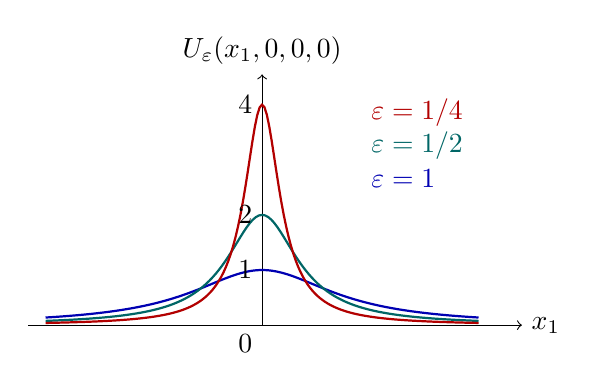
\begin{tikzpicture}[x=1.1cm,y=0.7cm]
	\draw[->] (-2.7,0)--(3.0,0) node[right] {\(x_1\)};
	\draw[->] (0,0)--(0,4.55) node[above] {\(U_\varepsilon(x_1,0,0,0)\)};
	\draw[thick,blue!70!black,domain=-2.5:2.5,samples=141] plot (\x,{1/(1+\x*\x)});
	\draw[thick,teal!80!black,domain=-2.5:2.5,samples=141] plot (\x,{0.5/(0.25+\x*\x)});
	\draw[thick,red!70!black,domain=-2.5:2.5,samples=181] plot (\x,{0.25/(0.0625+\x*\x)});
	\node[left] at (0,1) {\(1\)};
	\node[left] at (0,2) {\(2\)};
	\node[left] at (0,4) {\(4\)};
	\node[blue!70!black,right] at (1.15,2.65) {\(\varepsilon=1\)};
	\node[teal!80!black,right] at (1.15,3.25) {\(\varepsilon=1/2\)};
	\node[red!70!black,right] at (1.15,3.85) {\(\varepsilon=1/4\)};
	\node[below left] at (0,0) {\(0\)};
\end{tikzpicture}

	\caption[临界气泡的尺度变化]{四维时 \(U_\varepsilon(x)=\varepsilon/(\varepsilon^2+|x|^2)\) 的一条径向截面。三条曲线的峰高和宽度不同；保持不变的是四维积分 \(\int_{\mathbb R^4}U_\varepsilon^4\)，而非图中曲线下的平面面积。}
	\label{g3:fig:yamabe-bubbles}
\end{figure}

确定梯度能量的最小代价，需要如下锐形式。它是本节使用的外部分析结果；见\cite[定理3.3，第50页]{LeeParker1987Yamabe}。
\begin{theorem}[锐 Sobolev 不等式]\label{g3:thm:yamabe-sharp-euclidean}
	设 \(n\ge3\)，令
	\[
		Y_S\coloneqq n(n-1)\operatorname{Vol}(S^n,g_{\mathrm{rd}})^{2/n},
	\]
	其中 \(g_{\mathrm{rd}}\) 是截面曲率为一的圆球度量。对每个 \(v\in C_c^\infty(\mathbb R^n)\)，有
	\begin{equation}\label{g3:eq:yamabe-sharp-sobolev}
		Y_S\left(\int_{\mathbb R^n}|v|^p\,\mathrm dx\right)^{2/p}
		\le a_n\int_{\mathbb R^n}|\mathrm Dv|^2\,\mathrm dx.
	\end{equation}
	常数 \(Y_S\) 不能增大。不等式延伸到 \(C_c^\infty\) 关于梯度 \(L^2\) 范数的完备化，在该空间中，式\eqref{g3:eq:yamabe-euclidean-bubble}的函数取得等号。
\end{theorem}
锐常数及气泡等号由所引文献第3节提供。本节从这一精确版本出发，证明它对紧流形极小化序列的后果。完备化中的函数可由式\eqref{g3:eq:yamabe-sharp-sobolev}唯一地解释为 \(L^p\) 函数，因此上述延伸有明确的函数意义。

\begin{proposition}\label{g3:prop:yamabe-sphere-constant}
	对 \(n\ge3\) 的单位圆球，有 \(Y(S^n,[g_{\mathrm{rd}}])=Y_S\)。
\end{proposition}
\begin{proof}
	立体投影把去掉一点的圆球度量写成
	\[
		g_{\mathrm{rd}}=\rho^{4/(n-2)}g_{\mathrm{eucl}},\qquad
		\rho(x)=\left(\frac{2}{1+|x|^2}\right)^{(n-2)/2}.
	\]
	给定光滑 \(w\) 于圆球，记它在这个坐标中的表达仍为 \(w\)，并令 \(F=\rho w\)。\Cref{g3:prop:conformal-laplacian-covariance}的共形能量变换给出
	\[
		\int_{\mathbb R^n}|F|^p\,\mathrm dx
		=\int_{S^n}|w|^p\,\mathrm d\mu_{\mathrm{rd}},
		\qquad
		a_n\int_{\mathbb R^n}|\mathrm DF|^2\,\mathrm dx=E_{g_{\mathrm{rd}}}(w).
	\]
	为核对无穷远处的积分，圆球上的光滑性给出 \(F=O(r^{2-n})\)、\(\mathrm DF=O(r^{1-n})\)。取在 \(B_R\) 上为一、支于 \(B_{2R}\)、梯度不超过 \(C/R\) 的截断 \(\eta_R\)。则 \(\eta_RF\to F\) 于 \(L^p\)，且梯度差的平方积分为 \(O(R^{2-n})\)。因此可以先对紧支函数使用共形公式与分部积分，再令 \(R\to\infty\)；没有留下边界项。

	对 \(\eta_RF\) 应用锐 Sobolev 不等式并取极限，得到 \(Q_{g_{\mathrm{rd}}}(w)\ge Y_S\)。光滑稠密性把它推广到 \(H^1(S^n)\)。另一方面，\(s_{g_{\mathrm{rd}}}=n(n-1)\)，常函数一满足
	\[
		Q_{g_{\mathrm{rd}}}(1)
		=n(n-1)\operatorname{Vol}(S^n,g_{\mathrm{rd}})^{1-2/p}=Y_S.
	\]
	上下界一致。
\end{proof}

现在把气泡放进任意闭流形的一个小坐标球。这个构造同时给出上界与失紧序列，因而解释了为什么必须关注严格不等号。
\begin{proposition}\label{g3:prop:yamabe-bubble-upper-bound}
	设 \((M^n,g)\) 为闭连通光滑黎曼流形，\(n\ge3\)。则 \(Y(M,[g])\le Y_S\)。此外，存在非负 \(v_\varepsilon\in C^\infty(M)\)，满足
	\[
		\|v_\varepsilon\|_p=1,\qquad
		v_\varepsilon\rightharpoonup0\ \text{于 }H^1(M),\qquad
		Q_g(v_\varepsilon)\longrightarrow Y_S.
	\]
	这些函数没有 \(L^p\) 强收敛子列。
\end{proposition}
\begin{proof}
	取一点 \(x_0\) 的正规坐标球 \(B_{2r}(0)\)，以及在 \(B_r\) 上为一、支于 \(B_{2r}\) 的光滑非负截断 \(\chi\)。把 \(b_\varepsilon=\chi U_\varepsilon\) 搬到 \(M\)，在坐标球外补零。换元后，\(g_{ij}(\varepsilon y)\to\delta_{ij}\) 于每个固定球，且原坐标球上的度量与 Euclid 度量一致可比。利用 \(U_1^p\) 和 \(|\mathrm DU_1|^2\) 的可积性，先控制 \(|y|>R\) 的尾部，再令 \(\varepsilon\to0\)、\(R\to\infty\)，得到
	\[
		\int_M b_\varepsilon^p\,\mathrm d\mu_g\longrightarrow
		A\coloneqq\int_{\mathbb R^n}U_1^p\,\mathrm dx>0,
	\qquad
		\int_M|\mathrm db_\varepsilon|^2\,\mathrm d\mu_g
		\longrightarrow\int_{\mathbb R^n}|\mathrm DU_1|^2\,\mathrm dx.
	\]
	第二个极限中的截断误差支于固定环带，在那里 \(U_\varepsilon\) 及其导数均为 \(O(\varepsilon^{(n-2)/2})\)，故误差趋于零。

	零阶项要单独估计。径向积分给出
	\begin{equation}\label{g3:eq:yamabe-bubble-l2}
		\|b_\varepsilon\|_2^2\le C
		\begin{cases}
			\varepsilon,&n=3,\\
			\varepsilon^2\log(1/\varepsilon),&n=4,\\
			\varepsilon^2,&n\ge5,
		\end{cases}
	\end{equation}
	其中取 \(0<\varepsilon<\min\{r,1/2\}\)。例如换元后的积分是常数倍的
	\(\varepsilon^2\int_0^{2r/\varepsilon}t^{n-1}(1+t^2)^{-(n-2)}\,\mathrm dt\)；被积函数在无穷远处为 \(O(t^{3-n})\)，所以出现以上三种情形。由于 \(s_g\) 有界，\(\int s_gb_\varepsilon^2\to0\)。锐不等式在 \(U_1\) 上取等号，遂有 \(Q_g(b_\varepsilon)\to Y_S\)。

	取 \(v_\varepsilon=b_\varepsilon/\|b_\varepsilon\|_p\)。它们在 \(H^1\) 中有界而在 \(L^2\) 中趋于零，因此每个弱收敛子列的极限都为零，故整族弱趋于零。若存在 \(L^p\) 强收敛子列，它也在 \(L^2\) 中趋于同一极限零，与 \(L^p\) 范数恒为一矛盾。最后，由 \(Y(M,[g])\le Q_g(v_\varepsilon)\) 取极限即得上界。
\end{proof}

在任意远离 \(x_0\) 的紧集上，\(v_\varepsilon\) 及其梯度都趋于零；与此同时，\(\int v_\varepsilon^p=1\)。也就是说，体积密度 \(v_\varepsilon^p\,\mathrm d\mu_g\) 的质量集中到 \(x_0\)。这具体说明了临界约束为什么不由弱收敛保留。

\subsection{范数分裂与能量缺陷}
\label{g3:subsec:2404:02}
为处理一般极小化序列，并不需要预先证明它只含一个气泡。只要把弱极限与余项分开，给余项一个带锐常数的能量下界，就足以排除质量丢失。首先把 Euclid 不等式局部化；低阶误差留在 \(L^2\) 项中，而这个范数已有 Rellich 紧性。

\begin{lemma}\label{g3:lem:yamabe-near-sharp-sobolev}
	设 \((M^n,g)\) 为闭光滑黎曼流形，\(n\ge3\)。对每个 \(0<\delta<Y_S\)，存在 \(C_\delta\)，使每个 \(v\in H^1(M)\) 满足
	\begin{equation}\label{g3:eq:yamabe-near-sharp-sobolev}
		(Y_S-\delta)\|v\|_p^2
		\le a_n\|\mathrm dv\|_2^2+C_\delta\|v\|_2^2.
	\end{equation}
\end{lemma}
\begin{proof}
	以充分小的正规坐标球覆盖 \(M\)。度量系数及体积密度与 Euclid 值一致接近，故锐 Euclid 不等式与范数比较说明，对每个支于其中一球的 \(f\)，都有
	\[
		(Y_S-\delta)\|f\|_{L^p(g)}^2\le a_n\|\mathrm df\|_{L^2(g)}^2.
	\]
	这里选球的大小时，将两个比较因子的乘积控制得足够接近一，即可达到给定 \(\delta\)。取从属于有限覆盖的光滑函数 \(\eta_i\)，使 \(\sum_i\eta_i^2=1\)。它们可以从普通单位分解 \(\psi_i\) 构造为 \(\eta_i=\psi_i/(\sum_j\psi_j^2)^{1/2}\)。

	因为 \(p/2>1\)，\(L^{p/2}\) 的三角不等式给出
	\[
		\|v\|_p^2
		=\left\|\sum_i(\eta_iv)^2\right\|_{p/2}
		\le\sum_i\|\eta_iv\|_p^2.
	\]
	局部估计求和后，使用 \(\sum_i\eta_i\,\mathrm d\eta_i=0\)，得到精确恒等式
	\[
		\sum_i|\mathrm d(\eta_iv)|^2
		=|\mathrm dv|^2+v^2\sum_i|\mathrm d\eta_i|^2.
	\]
	最后一项的系数在紧流形上有界，吸收到 \(C_\delta\) 即得结论。先对光滑函数计算，再用 \(H^1\) 光滑稠密性与连续嵌入推广到全部 \(H^1\) 函数。
\end{proof}

下一条范数分裂说明，几乎处处收敛比单纯弱收敛多保留了什么：临界质量虽可能丢失，却可以准确归入余项。
\begin{lemma}\label{g3:lem:yamabe-norm-splitting}
	设 \((X,\mu)\) 为测度空间，\(1<q<\infty\)。若实函数列 \(f_j\) 在 \(L^q(X)\) 中有界，且几乎处处趋于 \(f\)，则 \(f\in L^q(X)\)，并有
	\begin{equation}\label{g3:eq:yamabe-norm-splitting}
		\int_X|f_j|^q\,\mathrm d\mu
		=\int_X|f|^q\,\mathrm d\mu
		+\int_X|f_j-f|^q\,\mathrm d\mu+o(1).
	\end{equation}
\end{lemma}
\begin{proof}
	Fatou 引理给出 \(f\in L^q\)，故 \(h_j=f_j-f\) 也在 \(L^q\) 中有界。对每个 \(\epsilon>0\)，中值公式和 Young 不等式给出
	\[
		\bigl||a+b|^q-|a|^q\bigr|
		\le\epsilon|a|^q+C_\epsilon|b|^q,
		\qquad a,b\in\mathbb R.
	\]
	具体地，中值公式先给出 \(C_q(|a|^{q-1}|b|+|b|^q)\)，再用共轭指数 \(q/(q-1)\) 与 \(q\) 即得所示形式。令
	\[
		d_j=|f_j|^q-|h_j|^q-|f|^q,
		\qquad r_j=(|d_j|-\epsilon|h_j|^q)_+.
	\]
	由于 \(h_j\to0\) 几乎处处，有 \(r_j\to0\) 几乎处处；上式又给 \(0\le r_j\le(C_\epsilon+1)|f|^q\)。支配收敛定理于是给出 \(\int r_j\to0\)。因此
	\[
		\limsup_j\int_X|d_j|\,\mathrm d\mu
		\le\epsilon\sup_j\|h_j\|_q^q.
	\]
	令 \(\epsilon\downarrow0\) 即得 \(d_j\to0\) 于 \(L^1\)，从而得到所需等式。
\end{proof}

\begin{lemma}\label{g3:lem:yamabe-energy-defect}
	设 \((M^n,g)\) 为闭光滑黎曼流形，\(n\ge3\)。设实函数 \(u_j\rightharpoonup u\) 于 \(H^1(M)\)，\(\|u_j\|_p=1\)，且 \(E_g(u_j)\to\ell\)。则
	\begin{equation}\label{g3:eq:yamabe-energy-defect}
		\ell\ge E_g(u)+Y_S(1-\|u\|_p^p)^{2/p}.
	\end{equation}
\end{lemma}
\begin{proof}
	由\cref{g3:thm:compact-bundle-rellich}，弱收敛列在 \(L^2\) 中强趋于 \(u\)；取子列后也几乎处处收敛。写 \(w_j=u_j-u\)。前一引理给出
	\[
		\|w_j\|_p^p\longrightarrow1-\|u\|_p^p\ge0.
	\]
	弱收敛使梯度交叉项趋于零，\(L^2\) 强收敛使所有含 \(s_g\) 的余项趋于零。因此
	\[
		E_g(u_j)=E_g(u)+a_n\|\mathrm dw_j\|_2^2+o(1).
	\]
	对 \(w_j\) 使用式\eqref{g3:eq:yamabe-near-sharp-sobolev}，先令 \(j\to\infty\)；因为 \(\|w_j\|_2\to0\)，得到
	\[
		\ell-E_g(u)\ge(Y_S-\delta)(1-\|u\|_p^p)^{2/p}.
	\]
	再令 \(\delta\downarrow0\)，得到结论。各个子列产生同一个不等式，所以取几乎处处收敛子列不影响断言。
\end{proof}

这就是本章所需的\term[jizhong jin xing]{集中紧性}[concentration compactness]估计：余项携带的临界质量为 \(1-\|u\|_p^p\)，它的能量至少为这份质量的 \(2/p\) 次幂乘以 \(Y_S\)。证明没有预设余项的空间形状，因而也涵盖多个区域中的集中。

\subsection{低于球面常数时排除集中}
\label{g3:subsec:2404:03}
记 \(Y=Y(M,[g])\)，并令 \(\alpha=2/p=(n-2)/n\in(0,1)\)。若 \(\|u_j\|_p=1\)、\(E_g(u_j)\to Y\)，能量缺陷估计与 \(E_g(u)\ge Y\|u\|_p^2\) 将给出
\begin{equation}\label{g3:eq:yamabe-mass-comparison}
	Y\ge Yt^\alpha+Y_S(1-t)^\alpha,
	\qquad t=\|u\|_p^p\in[0,1].
\end{equation}
这里 \(t=0\) 表示所有临界质量都离开弱极限，\(0<t<1\) 表示只保住一部分，\(t=1\) 表示没有丢失。下面的代数比较同时处理这三种可能。

\begin{lemma}\label{g3:lem:yamabe-threshold-exclusion}
	设 \(Y<Y_S\)、\(Y_S>0\)、\(0<\alpha<1\)。若 \(t\in[0,1]\) 满足式\eqref{g3:eq:yamabe-mass-comparison}，则 \(t=1\)。
\end{lemma}
\begin{proof}
	若 \(t=0\)，式子给出 \(Y\ge Y_S\)，矛盾。若 \(0<t<1\) 且 \(Y>0\)，则
	\[
		Yt^\alpha+Y_S(1-t)^\alpha
		>Y\bigl(t^\alpha+(1-t)^\alpha\bigr)>Y,
	\]
	因为 \(t^\alpha>t\)、\((1-t)^\alpha>1-t\)。若 \(Y\le0\)，则
	\[
		Yt^\alpha+Y_S(1-t)^\alpha-Y
		=Y(t^\alpha-1)+Y_S(1-t)^\alpha>0;
	\]
	第一项非负，第二项为正。这同样与假设矛盾。只剩 \(t=1\)。
\end{proof}

严格阈值有两个作用。全部集中时，代价 \(Y_S\) 已经高于极小值 \(Y\)；部分集中时，指数 \(\alpha<1\) 又使质量拆分增加代价。这解释了为何不必先定位集中点，也能证明极小化序列紧。

\subsection{严格阈值下的极小值实现}
\label{g3:subsec:2404:04}
\begin{theorem}\label{g3:thm:yamabe-below-sphere}
	设 \((M^n,g)\) 为闭连通光滑黎曼流形，\(n\ge3\)，且
	\[
		Y(M,[g])<Y(S^n,[g_{\mathrm{rd}}])=Y_S.
	\]
	则存在光滑正函数 \(u\)，使 \(\int_Mu^p\,\mathrm d\mu_g=1\)、\(E_g(u)=Y(M,[g])\)。它满足
	\[
		L_gu=Y(M,[g])u^{p-1},
	\]
	度量 \(u^{4/(n-2)}g\) 具有体积一和常标量曲率 \(Y(M,[g])\)。每个归一化的非负极小化序列，都有在 \(H^1(M)\) 中强收敛到某个这样的极小函数的子列。
\end{theorem}
\begin{proof}
	记 \(Y=Y(M,[g])\)，取非负极小化序列 \(u_j\)，满足 \(\|u_j\|_p=1\)。Hölder 不等式给出 \(\|u_j\|_2^2\le\operatorname{Vol}(M,g)^{2/n}\)，而
	\[
		a_n\|\mathrm du_j\|_2^2
		\le E_g(u_j)+\|s_g^-\|_\infty\|u_j\|_2^2,
		\qquad s_g^-=\max\{-s_g,0\}.
	\]
	故 \(u_j\) 在 \(H^1\) 中有界。取弱收敛子列 \(u_j\rightharpoonup u\)，由 Rellich 紧性进一步取 \(L^2\) 及几乎处处收敛子列。因此 \(u\ge0\)，且 \(t=\|u\|_p^p\le1\)。

	由能量缺陷估计以及 Yamabe 常数的定义，得到式\eqref{g3:eq:yamabe-mass-comparison}；当 \(u=0\) 时，\(E_g(u)\ge Y\|u\|_p^2\) 也成立。\Cref{g3:lem:yamabe-threshold-exclusion}给出 \(t=1\)。于是 \(u\) 保留全部约束，且
	\[
		Y\le E_g(u)\le\liminf_jE_g(u_j)=Y.
	\]
	这里第二个不等式使用梯度范数弱下半连续性与势能项的 \(L^2\) 连续性。所以 \(u\) 取得极小值。

	还有强收敛。由 \(E_g(u_j)\to E_g(u)\) 及 \(L^2\) 强收敛，得到 \(\|\mathrm du_j\|_2\to\|\mathrm du\|_2\)。Hilbert 空间中的弱收敛与范数收敛推出梯度强收敛，结合 \(L^2\) 收敛即得 \(H^1\) 强收敛。连续 Sobolev 嵌入同时给出 \(L^p\) 强收敛。

	\Cref{g3:prop:yamabe-euler-lagrange}的约束变分给出所示弱方程，\(u\not\equiv0\)。\Cref{g3:thm:yamabe-weak-regularity}把它提升为光滑正解；共形标量曲率及体积公式给出度量的结论。对任意归一化非负极小化序列，上述步骤都适用，故也得到最后的紧性断言。
\end{proof}

\begin{example}\label{g3:exm:yamabe-threshold-sharpness}
	在圆球上，\(Y=Y_S\)，极小值已由常函数取得；但\cref{g3:prop:yamabe-bubble-upper-bound}给出的截断气泡仍是归一化极小化序列，并且弱趋于零。因此，极小值存在不意味着所有极小化序列紧。严格阈值定理同时证明存在性与序列紧性，而等号情形至少需要另行处理其中的集中行为。
\end{example}

至此，剩余问题集中为一个几何比较：除圆球共形类之外，如何把某个测试函数的商压到 \(Y_S\) 以下？普通坐标中的截断气泡只给极限上界；严格改进要使用曲率展开或 Green 函数的整体信息。
% 纲要条目排为编号小节标题，并进入目录与书签；说明段仍保留于纲要注释中。

% !TeX root = ../../Book3.tex
% 纲要标题：### 24.5 Yamabe 问题的一般存在性
% 纲要位置：几何学计划纲要.md，第 3156 行。
% 正文状态：初稿，尚未正式审核。

% 纲要内容开始
% 
% * Aubin 型测试函数
% * 低维与局部共形平坦情形
% * 正质量定理与 Schoen 方法
% * 局部极小、全局极小和非唯一解
% 
% ---
% 
% 纲要内容结束

\section{Yamabe 问题的一般存在性}
\label{g3:sec:2405}

严格阈值定理把一般存在性归结为一个具体问题：当共形类不是圆球面的共形类时，怎样找出一个满足 \(Q_g(v)<Y_S\) 的测试函数？截断气泡只给出趋近球面常数的函数列。要使商严格下降，还须读出气泡所处几何对能量的下一阶贡献。局部曲率足以处理一部分情形，剩下的情形则需要把测试函数延伸到整个流形。

\subsection{Aubin 型测试函数}
\label{g3:subsec:2405:01}
第3章的\cref{g3:prop:conformal-weyl}说明，四阶协变 Weyl 张量在 \(\widehat g=e^{2f}g\) 下变为 \(e^{2f}W_g\)。因此 \(W_g(q)\ne0\) 不能靠改变共形代表消去。Aubin 的测试函数利用这一点：先选择共形代表，使法坐标中的低阶体积误差尽量消失，再把径向气泡放在 \(W_g\ne0\) 的点附近。下面所引定理包括这一共形规范的构造和曲率项的符号计算。

\begin{theorem}[Aubin 的严格不等式]\label{g3:thm:yamabe-aubin-strict}
	记 \(Y_S=n(n-1)\operatorname{Vol}(S^n,g_{\mathrm{rd}})^{2/n}\)，\(g_{\mathrm{rd}}\) 为曲率一的圆球度量。
	设 \((M^n,g)\) 是闭连通光滑黎曼流形，\(n\ge6\)。若 \((M,g)\) 不是局部共形平坦的，则
	\[
		Y(M,[g])<Y_S.
	\]
	这里局部共形平坦是指每点都有邻域，在该邻域内 \(g\) 是某个 Euclid 度量的正光滑函数倍数。
\end{theorem}
这一结果及其与 Weyl 张量的关系见\cite[定理B，第39页；第5、11节]{LeeParker1987Yamabe}。所用的局部共形平坦判别是 \(n\ge4\) 时 \(W\equiv0\) 当且仅当局部共形平坦；本卷第3章已经证明其中由局部共形平坦推出 \(W=0\) 的方向，反方向及测试函数的高阶规范在这里随外部结果调用。

\ProseParagraphBreak
维数 \(6\) 的分界可以从一个径向积分看出。取
\[
	U_\varepsilon(r)=\left(\frac{\varepsilon}{\varepsilon^2+r^2}\right)^{(n-2)/2},
	\qquad 0<\varepsilon<\rho,
\]
其中 \(\rho\) 固定。记 \(\sigma_{n-1}=\operatorname{Vol}(S^{n-1})\)。计算局部曲率修正时会遇到
\begin{equation}\label{g3:eq:yamabe-curvature-moment}
	\int_{B_\rho}|x|^2U_\varepsilon^2\,\mathrm dx
	=\sigma_{n-1}\varepsilon^4
	\int_0^{\rho/\varepsilon}\frac{t^{n+1}}{(1+t^2)^{n-2}}\,\mathrm dt.
\end{equation}
等式由极坐标和 \(r=\varepsilon t\) 直接得到。被积函数在无穷远与 \(t^{5-n}\) 同阶，所以 \(n\ge7\) 时右侧与 \(\varepsilon^4\) 同阶，\(n=6\) 时则与 \(\varepsilon^4\log(1/\varepsilon)\) 同阶。另一方面，固定环带内截断气泡的梯度误差是 \(O(\varepsilon^{n-2})\)。前两种曲率修正都能支配截断误差；外引定理的关键计算进一步说明，经过共形规范后，非零 Weyl 曲率贡献所需的下降方向。尺度比较解释了这个计算为何可能成功，下降的符号则来自完整的曲率展开。

\subsection{低维与局部共形平坦情形}
\label{g3:subsec:2405:02}
对 \(n=3,4,5\)，式\eqref{g3:eq:yamabe-curvature-moment}分别与 \(\varepsilon\)、\(\varepsilon^2\)、\(\varepsilon^3\) 同阶，恰与 \(\varepsilon^{n-2}\) 的截断误差处于同一尺度。缩小气泡便不能单凭阶数把误差压到主项以下。在局部共形平坦情形，困难更直接：可以选取在一个小球内完全平坦的共形代表，这时只支于该球内的测试函数受到 Euclid 最佳 Sobolev 不等式的约束。

\begin{proposition}\label{g3:prop:yamabe-flat-local-tests}
	对所用度量 \(h\)，记 \(E_h(v)=\int_M(\tfrac{4(n-1)}{n-2}|\mathrm dv|_h^2+s_hv^2)\,\mathrm d\mu_h\)，\(Q_h(v)=E_h(v)/\|v\|_{L^{2n/(n-2)}(h)}^2\)（\(v\ne0\)）。记 \(Y_S=n(n-1)\operatorname{Vol}(S^n,g_{\mathrm{rd}})^{2/n}\)，\(g_{\mathrm{rd}}\) 为曲率一的圆球度量。
	设 \((M^n,g)\) 为光滑黎曼流形，\(n\ge3\)，且某开集 \(V\) 在坐标下的度量恰为 Euclid 度量。对每个非零 \(v\in C_c^\infty(V)\)，有
	\[
		Q_g(v)\ge Y_S.
	\]
	若在同一个坐标开集 \(V\) 上有 \(g=\phi^{4/(n-2)}g_{\mathrm E}\)、\(\phi>0\) 光滑，同一结论仍适用于支于 \(V\) 的测试函数。
\end{proposition}
\begin{proof}
	平坦情形下 \(s_g=0\)，把 \(v\) 经坐标送到 Euclid 空间并补零，\cref{g3:thm:yamabe-sharp-euclidean}给出
	\[
		Q_g(v)=\frac{a_n\int_{\mathbb R^n}|\mathrm dv|^2\,\mathrm dx}
		{(\int_{\mathbb R^n}|v|^p\,\mathrm dx)^{2/p}}
		\ge Y_S.
	\]
	一般情形写 \(g=\phi^{4/(n-2)}g_0\)，其中 \(g_0\) 在 \(V\) 上平坦，\(\phi>0\)。由\cref{g3:prop:conformal-laplacian-covariance}，对支于 \(V\) 的函数有 \(Q_g(v)=Q_{g_0}(\phi v)\)。函数 \(\phi v\) 仍紧支于 \(V\)，故归结为第一种情形。
\end{proof}
这解释了为何局部共形平坦流形的严格不等式必须看到小球之外的几何。球面空间形式在小邻域内与圆球面没有共形区别，整体的覆盖结构却能使 Yamabe 常数严格下降。

\begin{example}\label{g3:exm:yamabe-spherical-quotient}
	设 \(n\ge3\)，有限群 \(\Gamma\) 在曲率为一的圆球面 \((S^n,g_{\mathrm{rd}})\) 上自由、等距地作用。令 \(d=|\Gamma|\)，\(M=S^n/\Gamma\)，\(g\) 为诱导商度量，\(\pi:S^n\to M\) 为覆盖映射。记
	\[
		p=\frac{2n}{n-2},\qquad a_n=\frac{4(n-1)}{n-2},
		\qquad Y_S=n(n-1)\operatorname{Vol}(S^n,g_{\mathrm{rd}})^{2/n}.
	\]
	对所用度量 \(h\)，令
	\[
		E_h(v)=\int\bigl(a_n|\mathrm dv|_h^2+s_hv^2\bigr)\,\mathrm d\mu_h,
		\qquad Q_h(v)=\frac{E_h(v)}{\|v\|_{L^p(h)}^2}\quad(v\ne0).
	\]
	则商流形的 Yamabe 常数为
	\[
		Y(M,[g])=d^{-2/n}Y_S.
	\]
	为证明下界，取任意非零 \(u\in H^1(M)\)。覆盖映射是局部等距，每点有 \(d\) 个原像，所以按覆盖片积分得到
	\[
		E_{g_{\mathrm{rd}}}(u\circ\pi)=dE_g(u),
		\qquad
		\|u\circ\pi\|_{L^p(g_{\mathrm{rd}})}^2
		=d^{2/p}\|u\|_{L^p(g)}^2.
	\]
	这些公式可先对光滑函数验证，再由光滑函数在 \(H^1\) 中稠密及 Sobolev 嵌入推广到上述 \(u\)。因此
	\[
		Q_{g_{\mathrm{rd}}}(u\circ\pi)=d^{1-2/p}Q_g(u)
		=d^{2/n}Q_g(u).
	\]
	由\cref{g3:prop:yamabe-sphere-constant}，左侧至少为 \(Y_S\)，故对全部竞争函数都有 \(Q_g(u)\ge d^{-2/n}Y_S\)。另一方面，局部等距性给出 \(s_g=n(n-1)\)，且 \(\operatorname{Vol}_g(M)=\operatorname{Vol}(S^n,g_{\mathrm{rd}})/d\)，从而
	\[
		Q_g(1)=n(n-1)\bigl(\operatorname{Vol}(S^n,g_{\mathrm{rd}})/d\bigr)^{2/n}
		=d^{-2/n}Y_S.
	\]
	上下界一致，且常数函数实现极小值。若 \(d>1\)，所得常数严格小于 \(Y_S\)。商流形局部共形平坦，\cref{g3:prop:yamabe-flat-local-tests}却保证每个紧支于一个共形平坦坐标小球的非零测试函数仍满足 \(Q_g(v)\ge Y_S\)。所以这里的下降由遍及商流形的测试函数反映，不能只从一个小球内的几何得到。
\end{example}

\ProseParagraphBreak
延伸测试函数时，希望其在气泡之外的能量尽可能小。那里函数的值很小，方程中的 \(u^{p-1}\) 比 \(u\) 衰减更快，因此先求线性方程 \(L_gu=0\) 是自然的选择。带一个极点的正 Green 函数正好同时满足这个方程，并具有与气泡远场相匹配的 \(r^{2-n}\) 奇性。

\subsection{正质量定理与 Schoen 方法}
\label{g3:subsec:2405:03}
设 \(Y(M,[g])>0\)。固定 \(q\in M\)，将共形 Laplace 的 Green 函数归一化为
\begin{equation}\label{g3:eq:yamabe-green-normalization}
	L_gG_q=a_n(n-2)\sigma_{n-1}\delta_q,
	\qquad G_q(x)\sim d_g(x,q)^{2-n}.
\end{equation}
这里 Dirac 分布以 \(g\) 的体积密度解释。正性条件使 \(L_g\) 可逆；Green 函数的存在、严格正性及所需局部展开见\cite[引理6.1、6.4，定理6.5]{LeeParker1987Yamabe}。先看 \(g\) 在 \(q\) 附近平坦的情形，此时
\[
	G_q(x)=|x|^{2-n}+A_q+O(|x|).
\]
减去基本解后留下的是光滑调和函数，所以这里的余项也可逐次微分。定义穿孔流形上的度量
\begin{equation}\label{g3:eq:yamabe-green-blowup}
	g_\infty=G_q^{4/(n-2)}g
	\quad\text{于 }M\setminus\{q\}.
\end{equation}
由标量曲率变换公式，\(s_{g_\infty}=0\)。在 \(q\) 附近，径向长度与 \(r^{-2}\,\mathrm dr\) 可比，到 \(q\) 的距离无穷大；其余部分来自紧流形。故 \(g_\infty\) 完备，原来的点变成一个无穷远端。

\ProseParagraphBreak
作反演 \(y=x/|x|^2\)，记 \(R=|y|\)。Euclid 度量在反演下贡献 \(R^{-4}\)，它与 Green 函数主项的共形倍数抵消，得到
\begin{equation}\label{g3:eq:yamabe-green-af}
	(g_\infty)_{ij}(y)
	=\bigl(1+A_qR^{2-n}+O(R^{1-n})\bigr)^{4/(n-2)}\delta_{ij}.
\end{equation}
这类在无穷远趋于 Euclid 度量，并且一、二阶导数有相应衰减的度量称为\term[jianjinpingtanduoliang]{渐近平坦度量}[asymptotically flat metric]。在坐标满足
\(h_{ij}-\delta_{ij}=O(R^{-\tau})\)、其一、二阶导数分别为 \(O(R^{-\tau-1})\)、\(O(R^{-\tau-2})\)，其中 \(\tau>(n-2)/2\)，且标量曲率可积时，所用质量归一化为
\begin{equation}\label{g3:eq:yamabe-adm-mass}
	m(h)=\frac1{2(n-1)\sigma_{n-1}}
	\lim_{R\to\infty}\int_{|y|=R}
	\sum_{i,j}(\partial_jh_{ij}-\partial_ih_{jj})\nu^i\,\mathrm dS.
\end{equation}
法向和面积元在此按 Euclid 度量计算。在这组衰减与可积条件下，极限的存在及坐标不变性可由\cite[第9节，定理9.6]{LeeParker1987Yamabe}核对；该文的质量比式\eqref{g3:eq:yamabe-adm-mass}大 \(2(n-1)\) 倍。对式\eqref{g3:eq:yamabe-green-af}，令括号的 \(4/(n-2)\) 次幂为 \(f\)，便有
\[
	\sum_j(\partial_jh_{ij}-\partial_ih_{jj})
	=-(n-1)\partial_if,
	\qquad
	\partial_R f=-4A_qR^{1-n}+O(R^{-n}),
\]
从而直接算得
\begin{equation}\label{g3:eq:yamabe-mass-green-coefficient}
	m(g_\infty)=2A_q.
\end{equation}
Green 函数的常数项因此记录了整个穿孔流形的几何，而不只是极点处有限阶的曲率。

\begin{theorem}\label{g3:thm:yamabe-green-positive-mass}
	设 \((M^n,g)\) 为闭连通光滑黎曼流形，\(n\ge3\)、\(Y(M,[g])>0\)，并满足以下条件之一：\(3\le n\le5\)；或 \((M,g)\) 局部共形平坦。任取 \(q\in M\)，在 \(q\) 附近先选择共形法坐标代表，局部共形平坦时可选为平坦代表，再按式\eqref{g3:eq:yamabe-green-normalization}归一化 Green 函数。令 \(g_\infty=G_q^{4/(n-2)}g\)，其中 \(G_q\) 是所选代表的上述归一化 Green 函数，\(m\) 为式\eqref{g3:eq:yamabe-adm-mass}的渐近平坦质量。则 \((M\setminus\{q\},g_\infty)\) 是完备、标量曲率为零的渐近平坦流形，其质量满足
	\[
		m(g_\infty)\ge0.
	\]
	质量为零当且仅当 \((M,[g])\) 与标准圆球面的共形类共形微分同胚；此时吹起度量等距于 Euclid 空间。
\end{theorem}
这里的共形法坐标可使体积密度在任意预先指定的有限阶上等于 Euclid 密度。低维时这一步保证渐近衰减足够快，并把质量与 Green 函数的常数项联系起来。对应的展开、质量联系与零质量刚性见\cite[引理6.4、9.7，第10节]{LeeParker1987Yamabe}及\cite[第2节，引理3、命题2]{Schoen1984Yamabe}。局部共形平坦的高维情形使用闭流形 Green 函数的特殊正质量结论，见\cite[命题3.3(i)、4.4，第62、65页]{SchoenYau1988ConformallyFlat}：先以第一特征函数选取正标量曲率代表，其覆盖空间上的标量曲率有正下界，四维所需的 Ricci 有界性也由紧性得到。这个版本只涉及上述 Green 函数吹起，不增加一般高维渐近平坦流形的假设范围。

\ProseParagraphBreak
若原流形不共形于球面，质量的严格正性提供了局部气泡没有的下降量。Schoen 把气泡的核心与小倍数 \(G_q\) 的远场接合，在环带中匹配两者。局部平坦时，分部积分把远场能量化为球面边界项，\(A_q>0\) 使关键边界项为负；先把接合半径取得足够小，再缩小气泡尺度，就能使接合误差小于这个负项。三维的一般 Green 展开仍能支持同样的构造；四、五维还需控制度量不平坦所产生的误差。精确的存在结论如下。

\begin{theorem}[Schoen 的严格不等式]\label{g3:thm:yamabe-schoen-strict}
	记 \(Y_S=n(n-1)\operatorname{Vol}(S^n,g_{\mathrm{rd}})^{2/n}\)，\(g_{\mathrm{rd}}\) 为曲率一的圆球度量。
	设 \((M^n,g)\) 为闭连通光滑黎曼流形，\(n\ge3\)。若 \(3\le n\le5\)，或 \((M,g)\) 局部共形平坦，并且 \((M,[g])\) 不共形微分同胚于标准圆球面的共形类，则
	\[
		Y(M,[g])<Y_S.
	\]
\end{theorem}
局部平坦附近的接合及三维情形见\cite[第1节，定理1、命题1，第481--484页]{Schoen1984Yamabe}；低维剩余估计及严格不等式见该文第2节、定理2（第493页）。其中作者把泛函除以了本章的 \(a_n\)，这个正因子不改变严格不等式。上述测试函数估计和正质量定理是本节外引的深层内容；下面的存在性结论只需把它们与已经证明的紧性相接。

\begin{corollary}[Yamabe 问题的一般存在性]\label{g3:cor:yamabe-general-existence}
	记 \(p=2n/(n-2)\)。共形 Laplace 算子取 \(L_g=\tfrac{4(n-1)}{n-2}\Delta_g+s_g\)，其中 \(\Delta_g=-\operatorname{div}_g\nabla\)。
	每个闭连通光滑黎曼流形 \((M^n,g)\)、\(n\ge3\)，都存在 \(u\in C^\infty(M)\)、\(u>0\)，使
	\[
		\int_Mu^p\,\mu_g=1,
		\qquad L_gu=Y(M,[g])u^{p-1}.
	\]
	因此 \(u^{4/(n-2)}g\) 是该共形类内体积为一、标量曲率恒等于 \(Y(M,[g])\) 的度量。
\end{corollary}
\begin{proof}
	若 \((M,[g])\) 是圆球面的共形类，取圆度量的拉回并作常数缩放，体积归一后即得结论。否则，在 \(n\ge6\) 且非局部共形平坦时应用\cref{g3:thm:yamabe-aubin-strict}，其余情形应用\cref{g3:thm:yamabe-schoen-strict}，均有 \(Y(M,[g])<Y_S\)。由\cref{g3:thm:yamabe-below-sphere}，存在归一化非负极小函数；\cref{g3:thm:yamabe-weak-regularity}将它提升为光滑正解。标量曲率与体积公式给出最后结论。
\end{proof}

\subsection{局部极小、全局极小和非唯一解}
\label{g3:subsec:2405:04}
上述存在性得到的是 Yamabe 泛函的全局极小值。一个任意的常标量曲率度量只保证泛函一阶变分为零，其二阶行为还要另行判断。为了把二阶条件写成普通 Laplace 谱，直接把待考察的常标量曲率度量作为背景度量。

\begin{proposition}\label{g3:prop:yamabe-csc-stability}
	记 \(p=2n/(n-2)\)。对所用度量 \(h\)，记 \(E_h(v)=\int_M(\tfrac{4(n-1)}{n-2}|\mathrm dv|_h^2+s_hv^2)\,\mathrm d\mu_h\)，\(Q_h(v)=E_h(v)/\|v\|_{L^{2n/(n-2)}(h)}^2\)（\(v\ne0\)）。
	设 \((M^n,g)\) 为闭连通光滑黎曼流形，\(n\ge3\)，\(\operatorname{Vol}_g(M)=1\)，且 \(s_g=s\) 为常数。令 \(\lambda_1(\Delta_g)\) 为标量 Laplace 的第一正特征值。函数 \(1\) 是约束 \(\int_M|v|^p\,\mu_g=1\) 上 \(E_g\) 的临界点，并有以下结论。
	\begin{enumerate}
		\item 若 \(1\) 是局部极小点，则 \(\lambda_1(\Delta_g)\ge s/(n-1)\)。
		\item 若 \(\lambda_1(\Delta_g)>s/(n-1)\)，则 \(1\) 是该约束集上相对于 \(H^1\) 拓扑的严格局部极小点。
		\item 若 \(\lambda_1(\Delta_g)<s/(n-1)\)，则存在保持体积的光滑正共形变化，使泛函在 \(g\) 附近严格下降。
	\end{enumerate}
\end{proposition}
\begin{proof}
	体积约束的切空间是 \(\int_Mh\,\mu_g=0\)。把 \(u=1\)、\(\lambda=s\) 代入\cref{g3:prop:yamabe-second-variation}，约束 Hessian 为
	\begin{equation}\label{g3:eq:yamabe-csc-hessian}
		2a_n\left(\int_M|\mathrm dh|^2\,\mu_g
		-\frac{s}{n-1}\int_Mh^2\,\mu_g\right),
	\end{equation}
	因为 \((p-2)/a_n=1/(n-1)\)。式\eqref{g3:eq:first-eigenvalue-mean-zero}正是平均值为零函数的 Rayleigh 商表述，故局部极小时 Hessian 非负给出第一项。若出现严格反向不等式，取第一特征函数 \(h\)，沿
	\[
		v_t=\frac{1+th}{\|1+th\|_p}
	\]
	变化。\(h\) 光滑有界，所以 \(|t|\) 足够小时 \(v_t>0\)；一阶导数为零而二阶导数为负，得到第三项。

	设谱隙为严格正。Poincar\'e 不等式使式\eqref{g3:eq:yamabe-csc-hessian}在平均值为零的子空间上至少为 \(c\|h\|_{H^1}^2\)，其中 \(c>0\)。映射 \(v\mapsto\int_M|v|^p\,\mu_g\) 在 \(H^1\) 上为 \(C^2\)，且在 \(1\) 处的导数是 \(h\mapsto p\int_Mh\,\mu_g\)，在常数方向可逆。\cref{g3:cor:banach-implicit-parameters}因此把约束集在 \(1\) 附近写成平均值为零子空间上的 \(C^2\) 图。把 \(E_g\) 限制到这个图，Taylor 公式给出
	\[
		E_g(v)-E_g(1)\ge\frac c4\|h\|_{H^1}^2>0
	\]
	对足够小的非零参数 \(h\) 成立，证明第二项。
\end{proof}
等号 \(\lambda_1=s/(n-1)\) 只说明存在二阶零方向。它可能来自共形对称，判断局部极小还需使用高阶信息或已知的全局极小性质。另一方面，严格局部极小控制的是一个邻域；全局极小还须比较远离该邻域的共形因子。

\begin{example}\label{g3:exm:yamabe-sphere-nonuniqueness}
	记 \(Y_S=n(n-1)\operatorname{Vol}(S^n,g_{\mathrm{rd}})^{2/n}\)，其中 \(g_{\mathrm{rd}}\) 为曲率一的圆球度量。
	设 \(n\ge3\)，令 \(\bar g\) 是体积为一的圆球面度量。以立体投影坐标 \(x\in\mathbb R^n\) 表示球面去掉一点，Euclid 伸缩 \(x\mapsto tx\)、\(t>0\)，延伸为球面的共形微分同胚 \(F_t\)，且
	\[
		F_t^*\bar g=v_t^{4/(n-2)}\bar g,
		\qquad
		v_t(x)=\left(\frac{t(1+|x|^2)}{1+t^2|x|^2}\right)^{(n-2)/2}.
	\]
	在被删去的点使用反演坐标，上式仍为光滑正函数。由于拉回保持总体积和标量曲率，\(\|v_t\|_p=1\)、\(Q_{\bar g}(v_t)=Y_S\)。\(t\ne1\) 时 \(v_t\) 非常数，故同一个正 Yamabe 共形类内，体积为一的极小函数和作为固定流形上张量的极小度量都不唯一。这些度量彼此等距；若再模去共形微分同胚，它们属于同一类。
\end{example}

\begin{example}\label{g3:exm:yamabe-long-cylinder}
	设 \(n\ge3\)、\(L>0\)。在 \(S_L^1\times S^{n-1}\) 上取乘积度量，圆周长度为 \(L\)，球面半径为一。其标量曲率为 \((n-1)(n-2)\)。函数 \(h(t,\theta)=\cos(2\pi t/L)\) 的平均值为零，Rayleigh 商为 \((2\pi/L)^2\)。若
	\[
		L>\frac{2\pi}{\sqrt{n-2}},
	\]
	式\eqref{g3:eq:yamabe-csc-hessian}在这个方向为负。把度量缩放到体积一时，标量曲率和 Laplace 特征值乘以相同因子，负号保持不变。因此该乘积度量虽是常标量曲率度量，却不是所在共形类的局部极小度量。一般存在性推论保证该共形类另有一个全局极小度量。
\end{example}
正情形的三个问题由此分开：Euler--Lagrange 方程决定临界点，约束 Hessian 检验局部稳定性，而严格球面阈值和极小化序列的紧性给出全局极小值。体积约束只消去常数缩放，不能消去球面的非平凡共形对称。
% 纲要条目排为编号小节标题，并进入目录与书签；说明段仍保留于纲要注释中。


\begin{chaptersummary}
	在 \(n\ge3\) 维，共形变化 \(g_u=u^{4/(n-2)}g\) 使体积变为 \(u^p\mu_g\)，标量曲率变为 \(u^{1-p}L_gu\)，其中 \(p=2n/(n-2)\)、\(L_g=4(n-1)\Delta_g/(n-2)+s_g\)。共形能量满足 \(E_{g_u}(v)=E_g(uv)\)，所以 Yamabe 常数只依赖指定共形类。体积约束产生的乘子就是极小度量的常标量曲率。

	\ProseParagraphBreak
	非负弱解首先属于临界 Sobolev 空间。将方程写成 \(\Delta_gu=Vu\)，截断测试和 \(L^{n/2}\) 尾部吸收提高其可积指数，继而椭圆估计、强最大值原理和光滑复合给出光滑正解。最低特征值与 Yamabe 常数同号；线性核、常数缩放和非线性唯一性分别由不同条件决定。

	\ProseParagraphBreak
	当 \(Y\le0\) 时，归一化极小化序列的弱极限非零，能量等号恢复强 \(H^1\) 收敛。所得单位体积常标量曲率度量在共形类中唯一。正情形需要球面阈值：临界气泡保持梯度能量和 \(L^p\) 质量，近锐 Sobolev 估计则把丢失的质量换成至少为球面常数所决定的能量代价。范数分裂与极小性共同排除全部或部分集中，从而证明 \(Y<Y_S\) 时的极小值实现和极小化序列紧性。

	\ProseParagraphBreak
	一般存在性还需要严格阈值的几何来源。非局部共形平坦的高维情形使用 Weyl 曲率对气泡能量的修正，低维或局部共形平坦情形使用 Green 函数吹起与正质量。准确调用这些结果后，除圆球共形类外均落入严格阈值；圆球自身有显式极小度量。正情形的解可以不唯一，常标量曲率度量也可以不是局部极小点，约束 Hessian 和明确的共形模型分别揭示这两种现象。
\end{chaptersummary}

\BookExercises

\begin{exercise}\label{g3:ex:yamabe-background-scaling}
	设 \(c>0\)，令 \(h=c^2g\)。证明
	\[
		L_h=c^{-2}L_g,\quad E_h(u)=c^{n-2}E_g(u),\quad
		\|u\|_{L^p(h)}^2=c^{n-2}\|u\|_{L^p(g)}^2.
	\]
	求 \(Y(M,[h])\) 与 \(\lambda_1(L_h)\)，并说明为什么二者的尺度行为不同。
\end{exercise}
\begin{solution}
	常数缩放不改变 Levi--Civita 联络，逆度量乘以 \(c^{-2}\)，故 \(\Delta_h=c^{-2}\Delta_g\)、\(s_h=c^{-2}s_g\)，从而得到算子公式。体积密度乘以 \(c^n\)，能量的每一项遂乘以 \(c^{n-2}\)。范数平方乘以 \(c^{2n/p}=c^{n-2}\)，因此商不变，\(Y(M,[h])=Y(M,[g])\)。而 \(L^2\) 范数平方乘以 \(c^n\)，Rayleigh 商给出 \(\lambda_1(L_h)=c^{-2}\lambda_1(L_g)\)。Yamabe 常数已经消除了整体长度尺度，线性特征值仍具有长度平方的倒数这一尺度。
\end{solution}

\begin{exercise}\label{g3:ex:yamabe-prescribed-sign-obstruction}
	设 \(\phi>0\) 为 \(L_g\) 的第一特征函数。如果某个光滑函数 \(f\) 能写成 \(s_{u^{4/(n-2)}g}\)，其中 \(u>0\) 光滑，证明
	\[
		\int_M f\phi u^{p-1}\,\mu_g=\lambda_1(L_g)\int_M\phi u\,\mu_g.
	\]
	由此分别说明 \(Y>0\)、\(Y<0\)、\(Y=0\) 对目标函数 \(f\) 的必要符号限制。
\end{exercise}
\begin{solution}
	方程为 \(L_gu=fu^{p-1}\)。乘以 \(\phi\) 积分，并用自伴性和 \(L_g\phi=\lambda_1\phi\)，即得等式。右端的积分严格正，故当 \(Y>0\) 时左端为正，\(f\) 必须在某处为正；当 \(Y<0\) 时 \(f\) 必须在某处为负。当 \(Y=0\) 时左端为零，而权重 \(\phi u^{p-1}\) 处处正，所以 \(f\) 或恒为零，或必须变号。这些是必要条件，单靠该积分恒等式并不能构造满足条件的目标曲率。
\end{solution}

\begin{exercise}\label{g3:ex:yamabe-product-sign-transition}
	设 \(k,l\ge2\)，\((N^l,h)\) 为闭连通、截面曲率恒为 \(-1\) 的流形，\(n=k+l\)。在 \(S^k\times N\) 上取
	\(g_r=r^2g_{S^k}+h\)，其中单位球面度量记为 \(g_{S^k}\)。确定 \(Y(S^k\times N,[g_r])\) 的符号，并在非正情形求出它的值和单位体积 Yamabe 度量。
\end{exercise}
\begin{solution}
	乘积曲率公式给出常标量曲率
	\[
		s_r=\frac{k(k-1)}{r^2}-l(l-1),\qquad
		V_r=r^k\operatorname{Vol}(S^k,g_{S^k})\operatorname{Vol}(N,h).
	\]
	由于 \(\Delta_{g_r}\) 非负且常函数属于其核，\(\lambda_1(L_{g_r})=s_r\)。故 Yamabe 常数与 \(s_r\) 同号：在 \(r^2<k(k-1)/(l(l-1))\) 时为正，在等号处为零，在反向严格不等号时为负。非正情形由\cref{g3:prop:yamabe-nonpositive-constant-metric}得到 \(Y=s_rV_r^{2/n}\)，唯一的单位体积常标量曲率度量为 \(V_r^{-2/n}g_r\)。正情形的符号仍由第一特征值确定，但上述计算没有证明乘积度量是极小度量。
\end{solution}

\begin{exercise}\label{g3:ex:yamabe-implicit-nonpositive}
	设 \(g\) 为单位体积的常标量曲率度量，\(s_g=s\le0\)，取 \(r>n\)。证明：对足够小的 \(f\in L^r(M)\)，存在唯一接近 \((1,s)\) 的 \((u,\lambda)\in W^{2,r}(M)\times\mathbb R\)，满足
	\[
		L_gu=(f+\lambda)u^{p-1},\qquad \int_Mu^p\,\mu_g=1,\qquad u>0.
	\]
	说明这里的唯一性范围，以及 \(f\) 光滑时解的正则性。
\end{exercise}
\begin{solution}
	在正开集 \(\mathcal U_r\) 上定义
	\[
		\mathcal F(u,\lambda,f)=\left(L_gu-(f+\lambda)u^{p-1},\ \int_Mu^p\,\mu_g-1\right).
	\]
	Sobolev 复合及 \(W^{2,r}\to C^0\) 保证这是到 \(L^r\times\mathbb R\) 的光滑映射；其中 \(L^r\) 函数与有界连续函数的乘法连续。在 \((1,s,0)\) 处，关于 \((u,\lambda)\) 的微分为
	\[
		(h,\eta)\longmapsto\left(a_n\Delta_gh-(p-2)sh-\eta,\ p\int_Mh\,\mu_g\right).
	\]
	给定右端 \((F,b)\)，先由第二个分量设 \(h=b/p+h_0\)，\(\int h_0=0\)。第一分量积分后唯一确定
	\(\eta=-(p-2)sb/p-\int_MF\,\mu_g\)。剩下的方程是
	\[
		\bigl(a_n\Delta_g-(p-2)s\bigr)h_0=F-\int_MF\,\mu_g.
	\]
	在零均值空间，\(s\le0\) 与 Poincaré 不等式使左端的核为零。\cref{g3:thm:elliptic-fredholm-wkp}的椭圆 Fredholm 理论与自伴性给出满射，\(W^{2,r}\) 估计给出有界逆；当 \(s=0\) 时恰是限制在零均值空间的 Poisson 方程。于是原微分为 Banach 空间同构，\cref{g3:cor:banach-implicit-parameters}的隐函数定理得到所需解及其对 \(f\) 的光滑依赖。接近 \(1\) 的 \(W^{2,r}\) 函数有正下界，所以 \(u>0\)。唯一性只针对这个邻域内的 \((u,\lambda)\)；它没有比较远处的解。若 \(f\) 光滑，正下界和椭圆自举进一步给出 \(u\) 光滑。
\end{solution}

\begin{exercise}\label{g3:ex:yamabe-negative-prescribed-comparison}
	设 \((M^n,g)\) 闭且连通，\(n\ge3\)，\(f,h\in C^\infty(M)\) 满足 \(f\le h<0\)。假定正光滑函数 \(u,v\) 分别满足
	\[
		L_gu=fu^{p-1},\qquad L_gv=hv^{p-1},
		\qquad p=\frac{2n}{n-2}.
	\]
	证明 \(u\le v\)，并由此说明固定一个严格负的目标标量曲率函数时，正共形因子至多有一个。这里不要求体积归一化。
\end{exercise}
\begin{solution}
	令 \(\widetilde g=v^{4/(n-2)}g\)，其标量曲率为 \(h\)，并令 \(w=u/v>0\)。共形协变公式给出
	\[
		a_n\Delta_{\widetilde g}w+hw=fw^{p-1}.
	\]
	假设 \(w\) 的最大值大于一，并在 \(x_0\) 取得。此时 \(\Delta_{\widetilde g}w(x_0)\ge0\)，故
	\[
		f(x_0)w(x_0)^{p-2}\ge h(x_0).
	\]
	但 \(f(x_0)\le h(x_0)<0\) 且 \(w(x_0)>1\)，给出
	\(f(x_0)w(x_0)^{p-2}<f(x_0)\le h(x_0)\)，矛盾。因此 \(w\le1\)，即 \(u\le v\)。若两个目标函数相同，交换 \(u,v\) 再比较即得相等。目标函数的数值已固定了尺度，故此处无须另加体积条件。
\end{solution}

\begin{exercise}\label{g3:ex:yamabe-negative-curvature-bounds}
	设 \((M^n,g)\) 闭且连通，\(n\ge3\)，\(s_g<0\)，记 \(V=\operatorname{Vol}_g(M)\)、\(m=\min_Ms_g\)。证明
	\[
		mV^{2/n}\le Y(M,[g])
		\le V^{-(n-2)/n}\int_Ms_g\,\mu_g<0.
	\]
	证明左端或右端出现等号，当且仅当 \(s_g\) 为常数。
\end{exercise}
\begin{solution}
	对任意非零 \(v\in H^1(M)\)，梯度项非负，且
	\[
		E_g(v)\ge m\|v\|_2^2
		\ge mV^{2/n}\|v\|_p^2.
	\]
	取下确界得到下界，取竞争函数 \(v=1\) 得到上界。上界严格负，所以本节存在定理给出正光滑的单位范数极小元 \(u\)。

	若左端等号成立，则
	\[
		0=a_n\|\mathrm du\|_2^2
		+\int_M(s_g-m)u^2\,\mu_g
		+m\bigl(\|u\|_2^2-V^{2/n}\bigr).
	\]
	右侧三项都非负，故 \(u\) 是正常数，且 \(s_g=m\) 处处。若右端等号成立，则常函数是 \(Q_g\) 的极小元。将其归一化为 \(u=V^{-1/p}\)，Euler--Lagrange 方程给出 \(s_gu=Yu^{p-1}\)，故 \(s_g=YV^{-2/n}\) 为常数。反之，\(s_g\) 为负常数时，\cref{g3:prop:yamabe-nonpositive-constant-metric}说明两端同时取等号。
\end{solution}

\begin{exercise}\label{g3:ex:yamabe-disconnected-zero-nonuniqueness}
	令 \(M\) 为两个平坦 \(n\) 维环面 \((M_1,g_1)\)、\((M_2,g_2)\) 的不交并，\(n\ge3\)，并赋予分支度量 \(g\)。证明该共形类的 Yamabe 常数为零，却有无穷多个体积为一的标量平坦度量。说明哪些计算依旧成立，以及本节唯一性证明在哪一步使用了连通性。
\end{exercise}
\begin{solution}
	记 \(V_i=\operatorname{Vol}_{g_i}(M_i)\)。由于 \(s_g=0\)，\(E_g(u)=a_n\|\mathrm du\|_2^2\ge0\)，而正的分支常函数使能量为零，故 \(Y(M,[g])=0\)。对任意 \(t\in(0,1)\)，定义
	\[
		u_t|_{M_1}=\left(\frac{t}{V_1}\right)^{1/p},
		\qquad u_t|_{M_2}=\left(\frac{1-t}{V_2}\right)^{1/p}.
	\]
	这是正光滑函数，满足 \(L_gu_t=0\) 及 \(\int_Mu_t^p\,\mu_g=1\)。所以 \(u_t^{4/(n-2)}g\) 标量平坦且体积为一，两个分支的体积分别为 \(t\) 与 \(1-t\)，不同参数给出不同度量。

	梯度能量非负、常数竞争者和体积变换公式都仍适用。\(\Delta_gu=0\) 也仍推出 \(\mathrm du=0\)，但这只使 \(u\) 在每个连通分支上为常数。一个总体积约束不能同时固定两个正常数；唯一性证明正是在把分支常数变为一个全局常数时用了连通性。
\end{solution}

\begin{exercise}\label{g3:ex:yamabe-subcritical-bubble-norms}
	在闭 \(n\) 维流形 \((M,g)\) 上，\(n\ge3\)，取正文构造的归一化截断气泡 \(v_\varepsilon\)，其中心为 \(x_0\)。证明对每个 \(1\le q<p=2n/(n-2)\)，都有 \(\|v_\varepsilon\|_q\to0\)；再证明对每个连续函数 \(f\)，有
	\[
		\int_M f v_\varepsilon^p\,\mathrm d\mu_g\longrightarrow f(x_0).
	\]
	说明这两个结论为什么能够同时成立。
\end{exercise}
\begin{solution}
	已知 \(\|v_\varepsilon\|_2\to0\)、\(\|v_\varepsilon\|_p=1\)。当 \(1\le q\le2\) 时，有限体积上的 Hölder 不等式给出 \(\|v_\varepsilon\|_q\le\operatorname{Vol}(M)^{1/q-1/2}\|v_\varepsilon\|_2\to0\)。当 \(2<q<p\) 时，选 \(0<\theta<1\)，使 \(1/q=\theta/2+(1-\theta)/p\)，由插值有 \(\|v_\varepsilon\|_q\le\|v_\varepsilon\|_2^\theta\|v_\varepsilon\|_p^{1-\theta}\to0\)。

	对任意固定 \(\delta>0\)，截断气泡在 \(M\setminus B_\delta(x_0)\) 上一致为 \(O(\varepsilon^{(n-2)/2})\)，归一化分母趋于正数，故该区域的 \(p\) 次质量趋于零。又因总质量为一，
	\[
		\left|\int_M(f-f(x_0))v_\varepsilon^p\,\mathrm d\mu_g\right|
		\le\sup_{B_\delta(x_0)}|f-f(x_0)|
		+2\|f\|_\infty\int_{M\setminus B_\delta(x_0)}v_\varepsilon^p\,\mathrm d\mu_g.
	\]
	先令 \(\varepsilon\to0\)，再令 \(\delta\downarrow0\)，得到结论。低于临界指数的范数随集中而消失，临界幂却恰好补偿了支集缩小造成的损失，所以对应测度趋于点质量。
\end{solution}

\begin{exercise}\label{g3:ex:yamabe-two-bubbles-cost}
	在闭 \(n\) 维流形 \((M,g)\) 的两个互不相交坐标球内，分别构造归一化截断气泡 \(v_\varepsilon,w_\varepsilon\)，\(n\ge3\)。对固定 \(0<t<1\)，令
	\[
		z_\varepsilon=t^{1/p}v_\varepsilon+(1-t)^{1/p}w_\varepsilon.
	\]
	计算 \(\|z_\varepsilon\|_p\) 及 \(\lim Q_g(z_\varepsilon)\)。进而求两份相等质量及 \(k\) 份相等质量的集中能量极限。
\end{exercise}
\begin{solution}
	两族函数的支集不相交，所以 \(\int z_\varepsilon^p=t+(1-t)=1\)，且能量没有交叉项。记 \(\alpha=2/p=(n-2)/n\)，由单个气泡的能量极限得到
	\[
		Q_g(z_\varepsilon)=E_g(z_\varepsilon)
		=t^\alpha E_g(v_\varepsilon)+(1-t)^\alpha E_g(w_\varepsilon)
		\longrightarrow Y_S\bigl(t^\alpha+(1-t)^\alpha\bigr)>Y_S.
	\]
	当 \(t=1/2\) 时，极限为 \(2^{2/n}Y_S\)。同理，对 \(k\) 个不交坐标球中的归一化气泡，分别乘以 \(k^{-1/p}\) 后相加，所得函数仍有 \(L^p\) 范数一，能量极限为 \(k\cdot k^{-2/p}Y_S=k^{2/n}Y_S\)。质量拆成多个独立气泡比全部放在一个气泡中需要更多能量。
\end{solution}

\begin{exercise}\label{g3:ex:yamabe-near-sharp-coefficient}
	设 \((M^n,g)\) 为闭光滑黎曼流形，\(n\ge3\)。假定存在实常数 \(A,B\)，使对所有 \(v\in H^1(M)\)，都有
	\[
		\|v\|_p^2\le A\|\mathrm dv\|_2^2+B\|v\|_2^2.
	\]
	证明 \(A\ge a_n/Y_S\)，并证明 \(B\ge\operatorname{Vol}(M,g)^{-2/n}\)。说明这两个必要条件分别由怎样的函数检测。
\end{exercise}
\begin{solution}
	取归一化截断气泡 \(v_\varepsilon\)。其 \(L^2\) 范数趋于零，而 \(a_n\|\mathrm dv_\varepsilon\|_2^2\to Y_S\)，故令 \(\varepsilon\to0\) 得 \(1\le A Y_S/a_n\)，即 \(A\ge a_n/Y_S\)。这检测局部小尺度上的集中。

	再取常函数 \(v=1\)，梯度项消失，得到 \(\operatorname{Vol}(M)^{2/p}\le B\operatorname{Vol}(M)\)，即 \(B\ge\operatorname{Vol}(M)^{-2/n}\)。这检测整体的常数方向。两者都是必要条件；它们本身并没有证明同时取两个下界时不等式成立。
\end{solution}

\begin{exercise}\label{g3:ex:yamabe-explicit-positive-mass}
	设 \(n\ge3\)，\(0\le\rho\in C_c^\infty(\mathbb R^n)\)，令
	\[
		w(x)=1+\frac1{(n-2)\sigma_{n-1}}
		\int_{\mathbb R^n}\frac{\rho(y)}{|x-y|^{n-2}}\,\mathrm dy,
		\qquad h=w^{4/(n-2)}g_{\mathrm E}.
	\]
	证明 \(h\) 完备，计算其标量曲率和按式\eqref{g3:eq:yamabe-adm-mass}归一化的质量，并证明
	\[
		m(h)=\frac{2}{a_n(n-2)\sigma_{n-1}}
		\int_{\mathbb R^n}s_h w^{-1}\,\mu_h.
	\]
	说明在这个显式族中零质量意味着什么。
\end{exercise}
\begin{solution}
	在 \(\Delta_{\mathrm E}=-\sum_i\partial_i^2\) 的约定下，\(|x|^{2-n}/((n-2)\sigma_{n-1})\) 是基本解，故 \(\Delta_{\mathrm E}w=\rho\)。Newton 势与光滑紧支密度的卷积光滑，且 \(w\ge1\)，所以 \(h\ge g_{\mathrm E}\)。任何离开紧集的曲线都有无穷 Euclid 长度，因而也有无穷 \(h\) 长度，得到完备性。共形标量曲率公式给出
	\[
		s_h=a_nw^{1-p}\rho\ge0.
	\]
	因 \(\rho\) 紧支，\(|x|\to\infty\) 时对积分核展开得到
	\[
		w(x)=1+B|x|^{2-n}+O(|x|^{1-n}),
		\qquad B=\frac{\int\rho\,\mathrm dx}{(n-2)\sigma_{n-1}},
	\]
	一、二阶导数也有相应展开。代入质量积分，或重复式\eqref{g3:eq:yamabe-mass-green-coefficient}的径向计算，得 \(m(h)=2B\)。再由 \(\mu_h=w^p\,\mathrm dx\)，有
	\[
		\int s_hw^{-1}\,\mu_h
		=a_n\int\rho\,\mathrm dx,
	\]
	遂得所需恒等式。若质量为零，非负连续函数 \(\rho\) 的积分为零，故 \(\rho=0\)、\(w=1\)、\(h=g_{\mathrm E}\)。这个结论使用了给定的 Newton 势表示，只验证了这一显式族的正质量和刚性。
\end{solution}

\begin{exercise}\label{g3:ex:yamabe-spherical-quotient}
	设有限群 \(\Gamma\) 在单位圆球面 \(S^n\)、\(n\ge3\)，上自由、等距地作用，\(d=|\Gamma|\)，\(g\) 为商流形 \(M=S^n/\Gamma\) 的诱导度量。证明
	\[
		Y(M,[g])=d^{-2/n}Y_S.
	\]
	说明 \(d>1\) 时，这给出了何种严格不等式，以及为何它不能从支于一个共形坐标小球内的测试函数得到。
\end{exercise}
\begin{solution}
	记覆盖映射为 \(\pi:S^n\to M\)。对任意非零 \(u\in H^1(M)\)，局部等距性及覆盖次数给出
	\[
		E_{g_{S^n}}(u\circ\pi)=dE_g(u),
		\qquad
		\|u\circ\pi\|_p^2=d^{2/p}\|u\|_p^2.
	\]
	因此 \(Q_{g_{S^n}}(u\circ\pi)=d^{1-2/p}Q_g(u)=d^{2/n}Q_g(u)\)。球面的最佳常数给出 \(Q_g(u)\ge d^{-2/n}Y_S\)。另一方面，商度量的标量曲率为 \(n(n-1)\)，体积为 \(\operatorname{Vol}(S^n)/d\)，所以常数测试函数满足
	\[
		Q_g(1)=n(n-1)\bigl(\operatorname{Vol}(S^n)/d\bigr)^{2/n}
		=d^{-2/n}Y_S.
	\]
	上、下界一致。\(d>1\) 时所得常数严格小于 \(Y_S\)，且常数函数已经实现它。商流形局部共形平坦，\cref{g3:prop:yamabe-flat-local-tests}说明只支于一个共形平坦坐标小球的函数，其商仍不小于球面常数。这里的下降由遍及商流形的测试函数反映整体覆盖次数。
\end{solution}

\begin{exercise}\label{g3:ex:yamabe-product-negative-directions}
	对\cref{g3:exm:yamabe-long-cylinder}的乘积度量，令
	\[
		N_L=\#\left\{k\in\mathbb Z_{\ge1}:
		\left(\frac{2\pi k}{L}\right)^2<n-2\right\}.
	\]
	证明归一体积后，常数临界点的约束 Hessian 至少有 \(2N_L\) 个线性无关负方向。若 \(L=2\pi k_0/\sqrt{n-2}\)，说明所产生的两个二阶零方向，并解释为什么仅由它们不能断定出现了另一条常标量曲率度量族。
\end{exercise}
\begin{solution}
	对每个被计入 \(N_L\) 的整数 \(k\)，取
	\[
		c_k(t,\theta)=\cos(2\pi kt/L),
		\qquad s_k(t,\theta)=\sin(2\pi kt/L).
	\]
	这些函数的平均值均为零，彼此在 \(L^2\) 中正交；分部积分也使不同函数间的 Dirichlet 交叉项为零。\(c_k,s_k\) 的 Rayleigh 商都为 \((2\pi k/L)^2<n-2=s_g/(n-1)\)。所以式\eqref{g3:eq:yamabe-csc-hessian}在它们张成的 \(2N_L\) 维空间上负定。常数缩放度量只给二次型乘上正因子，不改变负方向的维数。

	若 \(L=2\pi k_0/\sqrt{n-2}\)，则 \(c_{k_0},s_{k_0}\) 的 Rayleigh 商恰等于 \(s_g/(n-1)\)，它们给出两个线性无关二阶零方向。由 Hessian 的极化公式，它们也与全部切方向在该二次型下正交，因而属于约束线性化的核。线性化有核只表示隐函数定理的可逆性条件在此失去；核中的向量是否能延伸成非线性方程的解曲线，还要检验高阶方程或使用适用的分支定理，不能从二阶为零直接推出。
\end{solution}

% !TeX root = ../../Book3.tex
% 纲要标题：## 第25章*　Einstein 方程、规范与局部模问题
% 纲要位置：几何学计划纲要.md，第 3165 行。
% 正文状态：初稿；尚未正式审核。

% 纲要内容开始
% 
% > 本章目标与证明范围：与 Yamabe 分章：Einstein 方程是模微分同胚的系统，而非标量共形方程。完整建立线性化、规范固定和有限维局部障碍模型；一般存在与分类不在本章无条件承诺。 非线性共同输入定位于 III.13.5—13.6，不以完整阅读 Yamabe 章为先修。
% 
% 纲要内容结束

\OptionalChapter{Einstein 方程、规范与局部模问题}{g3:ch:25}
\BookChapterNumber{g3:ch:25}

\begin{chapterabstract}
	Einstein 方程要求 Ricci 张量与度量成比例，而微分同胚使同一个几何对象具有无穷多个张量代表。本章从度量空间的切向量出发，推导联络、Ricci 张量、标量曲率及总体积的变分公式。随后用守恒的 Einstein 张量和背景散度构造椭圆方程，证明规范项在附近的解上消失，并通过核正交椭圆方程建立局部切片。形式自伴的线性化给出有限维无穷小形变空间；隐函数定理消去其正交补，剩下的有限维障碍映射及等距群作用描述局部模问题。空间形式、乘积和平坦环面分别说明刚性、可积形变、商空间与整体退化，Kähler 类中的 Ricci 平坦存在定理则作为明确的外部结果介绍。
\end{chapterabstract}

\begin{learninggoals}
	\begin{itemize}
		\item 在本卷曲率与 Laplace 符号约定下推导曲率线性化，并识别微分同胚产生的核方向。
		\item 计算带体积约束的 Einstein--Hilbert 泛函的一阶变分，区分固定常数、固定体积和模缩放问题。
		\item 验证规范化方程的椭圆性，证明规范等价与散度切片，并说明 Killing 场留下的剩余对称。
		\item 用 Fredholm 理论与隐函数定理构造有限维障碍映射，计算二阶障碍并判断局部刚性。
		\item 在空间形式、乘积和平坦环面上检验一般结论，区分局部参数、群作用和整体紧性。
	\end{itemize}
\end{learninggoals}

设 \(g_0\) 是圆球上的标准度量，\(\phi_t\) 是一族微分同胚。张量 \(\phi_t^*g_0\) 的坐标系数通常随 \(t\) 改变，但各个度量都与 \(g_0\) 等距。这种变化在微分后成为 \(\mathcal L_Xg_0\)。若把它当作真正改变几何的未知方向，曲率方程的线性化便出现一个由任意向量场产生的无限维核。研究附近的几何结构，首先要把这种重参数化自由处理清楚。

\ProseParagraphBreak
本章研究的条件是 \(\operatorname{Ric}_g=\lambda g\)，称为 Einstein 方程。\footnote{Albert Einstein（1879--1955），德国出生的理论物理学家，建立了广义相对论。}在维数至少为三的连通流形上，缩并 Bianchi 恒等式迫使这里的比例因子为常数。固定共形类的标量曲率问题只改变一个正函数；这里允许全部对称二张量方向变化，方程是一个带重参数化对称的系统。前一章的临界极小化论证不是本章的先修；直接使用的非线性工具来自第13.5—13.6节。

\ProseParagraphBreak
我们从一个已知的闭 Einstein 流形 \((M^n,g_0)\) 出发，问附近的解能否用有限个参数描述。先固定 Einstein 常数 \(\lambda\)，用散度条件选择代表，再用守恒恒等式证明所加的规范项确实消失。椭圆线性化的核与余核有限维，因而可以把无限维方程分解为一个可逆方向上的方程和一个有限维方程。后者可能有非零高阶项，所以无穷小形变不一定能延伸成真正的度量族；即使障碍消失，还须除去背景度量的等距群。

\ProseParagraphBreak
阅读时需要熟悉第1—3章的联络与曲率计算，以及第11—13章的 Sobolev、椭圆和 Banach 空间理论。正 Einstein 常数下的迹消去会调用第16章的第一特征值估计。固定常数、整体缩放与体积归一化的关系将在第25.3节末明确处理；最后一节用模型检验局部结论，并说明一般存在性与整体紧性还需要什么几何信息。

% !TeX root = ../../Book3.tex
% 纲要标题：### 25.1 度量空间和曲率变分
% 纲要位置：几何学计划纲要.md，第 3169 行。
% 正文状态：初稿；尚未正式审核。

% 纲要内容开始
% 
% * 对称二张量的切空间
% * Ricci 与标量曲率的线性化
% * 微分同胚方向的退化
% * Einstein–Hilbert 泛函和体积约束
% 
% 纲要内容结束

\section{度量空间和曲率变分}
\label{g3:sec:2501}

把度量的各个分量都作为未知函数，Ricci 曲率便成为一个含二阶导数的非线性算子。它和标量曲率方程有一个重要差别：改变坐标会同时改变全部度量分量，却不改变几何。为了看清这种退化，本节先在固定流形上求度量、联络和曲率的一阶变化，再把坐标变化放进同一公式。积分变分随后给出一个具有散度恒等式的 Einstein 方程；这一恒等式将在下一节帮助检验规范固定后的解。

以下积分均使用黎曼体积密度，因而不要求流形定向。除局部计算外，始终考虑闭连通光滑流形 \(M^n\)，\(n\ge3\)。对一个指定的光滑度量 \(g\)，\(\nabla\)、\(\operatorname{Ric}_g\)、\(s_g\) 分别表示其 Levi--Civita 联络、Ricci 张量和标量曲率。

\subsection{对称二张量的切空间}
\label{g3:subsec:2501:01}
在每一点，正定对称矩阵组成对称矩阵空间中的开凸锥。因此度量的变化方向不必正定；正定性限制的是变化后的度量，而不是切向量。

\begin{definition}\label{g3:def:einstein-metric-space}
	设 \(M^n\) 为闭连通光滑流形，\(n\ge3\)，\(g_0\) 为一个光滑黎曼度量，\(s>n/2+2\) 为整数。记
	\[
		\mathcal M^s(M)=\{g\in H^s(M;\operatorname{Sym}^2\mathrm T^*M):g(x)>0\text{ 对每个 }x\in M\}.
	\]
	其中 Sobolev 范数用 \(g_0\) 及其联络定义；连续代表由 Sobolev 嵌入唯一确定。若一个光滑度量 \(g\) 满足
	\begin{equation}\label{g3:eq:einstein-equation-fixed-lambda}
		\operatorname{Ric}_g=\lambda g
	\end{equation}
	且 \(\lambda\) 为实常数，就称 \(g\) 为\term[Einstein duliang]{Einstein 度量}[Einstein metric]，称 \(\lambda\) 为其 Einstein 常数。
\end{definition}

\begin{proposition}\label{g3:prop:metric-sobolev-open}
	设 \(M^n\) 为闭连通光滑流形，\(n\ge3\)，\(g_0\) 为光滑黎曼度量，\(s>n/2+2\) 为整数。则 \(\mathcal M^s(M)\) 是 \(H^s(M;\operatorname{Sym}^2\mathrm T^*M)\) 的开集，在任意 \(g\in\mathcal M^s(M)\) 处的切空间都是该对称二张量空间。映射
	\[
		g\longmapsto g^{-1},\qquad g\longmapsto\mu_g/\mu_{g_0}
	\]
	分别是到相应 \(H^s\) 截面空间的光滑映射。Ricci 张量与标量曲率给出光滑映射
	\[
		\operatorname{Ric}:\mathcal M^s(M)\longrightarrow H^{s-2}(M;\operatorname{Sym}^2\mathrm T^*M),
		\qquad
		\operatorname{Scal}:\mathcal M^s(M)\longrightarrow H^{s-2}(M).
	\]
\end{proposition}
\begin{proof}
	紧性使连续正定 \(g\) 相对于 \(g_0\) 的最小特征值有正下界 \(c\)。若 \(\|h\|_{C^0,g_0}<c\)，则 \(g+h\) 仍正定。第十一章的 Sobolev 嵌入给出 \(\|h\|_{C^0}\le C\|h\|_{H^s}\)，故正定条件在 \(H^s\) 中开。对每个对称张量 \(h\)，直线 \(g+th\) 在充分小的 \(|t|\) 上属于此开集，因而没有额外的切向限制。

	正定矩阵的求逆与行列式平方根是光滑纤维映射；在 \(g\) 的一个小邻域内，特征值一致远离零。将\cref{g3:thm:sobolev-composition-smooth}用于这些纤维映射，便得前两个光滑性结论。联络系数由 \(g^{-1}\partial g\) 的线性组合给出，曲率由 \(g^{-1}\partial^2g\) 及两个一阶导数的乘积给出，都是二阶喷射的光滑函数。由于 \(s-2>n/2\)，\cref{g3:prop:nonlinear-jet-operator}正好给出到 \(H^{s-2}\) 的光滑性。各图上的公式来自同一个张量，故按有限坐标覆盖粘合。
\end{proof}

这个开集描述也说明，光滑计算可以直接给出 Sobolev 映射的 Fréchet 导数：先在光滑方向上求导，再用已证的光滑性与稠密性延拓。所需的是固定源上的张量运算；变化坐标产生的复合另有导数计数。

\begin{lemma}\label{g3:lem:metric-inverse-volume-variation}
	设 \(M^n\) 为闭光滑流形，\(g(t)\) 为一条光滑黎曼度量曲线，\(g(0)=g\)、\(\dot g(0)=h\)，并记 \(H=\operatorname{tr}_g h\)。则
	\begin{equation}\label{g3:eq:inverse-volume-variation}
		\left.\frac{\mathrm d}{\mathrm dt}\right|_0g(t)^{ij}=-h^{ij},
		\qquad
		\left.\frac{\mathrm d}{\mathrm dt}\right|_0\mu_{g(t)}=\frac12H\mu_g.
	\end{equation}
	因此 \(V(g)=\int_M\mu_g\) 满足
	\[
		\mathrm DV_g(h)=\frac12\int_MH\,\mu_g.
	\]
\end{lemma}
\begin{proof}
	微分 \(g(t)^{ia}g(t)_{aj}=\delta^i_j\)，得到逆矩阵公式。体积密度在坐标中是 \(\sqrt{\det g(t)}\,|\mathrm dx^1\cdots\mathrm dx^n|\)。行列式的导数公式给出
	\[
		\left.\frac{\mathrm d}{\mathrm dt}\right|_0\log\det g(t)=\operatorname{tr}(g^{-1}h)=H,
	\]
	再微分平方根便得第二式。紧性允许在积分号下求导。
\end{proof}

例如 \(g(t)=(1+t)g\) 的切向量是 \(h=g\)，体积变化率为 \(nV(g)/2\)。固定体积的切向条件则只要求 \(\int H\,\mu_g=0\)，并不要求 \(H\) 在每一点为零；这两个条件将在形变计算中承担不同职责。

\subsection{Ricci 与标量曲率的线性化}
\label{g3:subsec:2501:02}
联络变化含一个度量导数，曲率变化再多一个导数。将这两步分开，可以保留协变形式，也能避免把指标升降中的变化混入曲率本身。

\begin{lemma}\label{g3:lem:levi-civita-variation}
	设 \(g(t)\) 为光滑流形 \(M\) 上的一条光滑黎曼度量曲线，\(g(0)=g\)、\(\dot g(0)=h\)。令
	\[
		C(X,Y)=\left.\frac{\mathrm d}{\mathrm dt}\right|_0\nabla^{g(t)}_XY
	\]
	其中 \(X,Y\) 固定而不随 \(t\) 变化。则 \(C\) 是对称的 \((1,2)\) 型张量，且
	\begin{equation}\label{g3:eq:connection-variation}
		2g(C(X,Y),Z)=(\nabla_Xh)(Y,Z)+(\nabla_Yh)(X,Z)-(\nabla_Zh)(X,Y).
	\end{equation}
	在坐标中，
	\[
		C^k_{ij}=\frac12g^{ka}\bigl(\nabla_i h_{ja}+\nabla_j h_{ia}-\nabla_a h_{ij}\bigr).
	\]
\end{lemma}
\begin{proof}
	两条联络之差是张量，微分仍保留张量性；无挠性给出 \(C(X,Y)=C(Y,X)\)。微分度量相容式，整理出
	\[
		(\nabla_Xh)(Y,Z)=g(C(X,Y),Z)+g(Y,C(X,Z)).
	\]
	将 \((X,Y,Z)\) 分别换成 \((Y,X,Z)\)、\((Z,X,Y)\)，把前两式相加再减去第三式。利用 \(C\) 的对称性，其余项相消，得到所需公式。
\end{proof}

下面固定所有收缩和伴随的符号。对对称二张量 \(h\) 与一形式 \(\omega\)，定义
\begin{equation}\label{g3:eq:divergence-bianchi-conventions}
	(\delta_g h)_j=-\nabla^i h_{ij},\qquad
	(\delta_g^*\omega)_{ij}=\frac12(\nabla_i\omega_j+\nabla_j\omega_i),\qquad
	\beta_g h=\delta_g h+\frac12\mathrm d\operatorname{tr}_g h.
\end{equation}
在一形式上，\(\delta_g\omega=-\nabla^i\omega_i\)，所以 \(\delta_g\mathrm df=\Delta_g f\)。闭流形上的分部积分说明 \(\delta_g^*\) 正是 \(\delta_g\) 的 \(L^2(g)\) 伴随。\(\beta_g\) 称为 \term[Bianchi suanzi]{Bianchi 算子}[Bianchi operator]；本节先用它组织曲率的导数。

对一点处的正交单位标架 \((e_a)\)，记
\begin{equation}\label{g3:eq:curvature-action-symmetric-tensors}
	\begin{aligned}
		\bigl(\mathring R_g(h)\bigr)_{ij}
		&=\sum_{a,b}h_{ab}\,g(R(e_a,e_i)e_j,e_b),\\
		\Delta_Lh&=\nabla^*\nabla h+\operatorname{Ric}_g\circ h+h\circ\operatorname{Ric}_g-2\mathring R_g(h).
	\end{aligned}
\end{equation}
这里 \((\operatorname{Ric}_g\circ h)_{ij}=\operatorname{Ric}_i{}^a h_{aj}\)，\(\nabla^*\nabla\) 使用非负主符号；后一算子称为\term[Lichnerowicz Laplace suanzi]{Lichnerowicz Laplace 算子}[Lichnerowicz Laplacian]。曲率的对称性保证这些定义与正交标架无关，并给出
\[
	\mathring R_g(g)=\operatorname{Ric}_g,\qquad
	\operatorname{tr}_g\mathring R_g(h)=\langle\operatorname{Ric}_g,h\rangle_g,
	\qquad \operatorname{tr}_g\Delta_Lh=\Delta_g\operatorname{tr}_g h.
\]
特别地，\(\Delta_Lg=0\)。这些检验固定了曲率作用中的槽位顺序。

\begin{theorem}\label{g3:thm:ricci-scalar-linearization}
	设 \(g(t)\) 为光滑流形 \(M\) 上的一条光滑黎曼度量曲线，\(g(0)=g\)、\(\dot g(0)=h\)，\(H=\operatorname{tr}_g h\)。曲率符号采用本书约定，\(\delta_g,\beta_g,\Delta_L\) 由式\eqref{g3:eq:divergence-bianchi-conventions}、\eqref{g3:eq:curvature-action-symmetric-tensors}定义。则
	\begin{align}
		\mathrm D\operatorname{Ric}_g(h)&=\frac12\Delta_Lh-\delta_g^*\beta_g h,\label{g3:eq:ricci-linearization}\\
		\mathrm D\operatorname{Scal}_g(h)&=\Delta_gH+\delta_g\delta_g h-\langle\operatorname{Ric}_g,h\rangle_g.\label{g3:eq:scalar-linearization}
	\end{align}
\end{theorem}
\begin{proof}
	先保持 Ricci 张量的两个指标都在下方。微分曲率坐标式\eqref{g3:eq:curvature-coordinate-components}，或在一点取 \(g\) 的法坐标，得
	\[
		(\mathrm D\operatorname{Ric}_g h)_{ij}=\nabla_k C^k_{ij}-\nabla_i C^k_{kj}.
	\]
	由 \(C^k_{kj}=\tfrac12\nabla_jH\)，得到尚未交换协变导数的表达
	\begin{equation}\label{g3:eq:ricci-linearization-uncommuted}
		2(\mathrm D\operatorname{Ric}_g h)_{ij}
		=\nabla_k\nabla_i h_j{}^k+\nabla_k\nabla_j h_i{}^k-\nabla_k\nabla^k h_{ij}-\nabla_i\nabla_jH.
	\end{equation}
	这里 \(h_j{}^k=g^{ka}h_{ja}\)，升指标使用固定的 \(g\)。对一个上指标和一个下指标，协变导数的交换分别给出正、负曲率作用，因而
	\[
		\nabla_k\nabla_i h_j{}^k
		=\nabla_i\nabla_k h_j{}^k+\operatorname{Ric}_i{}^a h_{aj}-\bigl(\mathring R_g(h)\bigr)_{ij}.
	\]
	另一项交换 \(i,j\) 后相同。将 \(\nabla_kh_j{}^k=-(\delta_gh)_j\) 代回式\eqref{g3:eq:ricci-linearization-uncommuted}，便有
	\[
		2\mathrm D\operatorname{Ric}_g(h)
		=\Delta_Lh-2\delta_g^*\delta_gh-\operatorname{Hess}_gH
		=\Delta_Lh-2\delta_g^*\beta_gh.
	\]
	因为 \(\delta_g^*\mathrm dH=\operatorname{Hess}_gH\)，得到第一式。

	标量曲率是 \(g^{ij}\operatorname{Ric}_{ij}\)，所以还要微分逆度量。由式\eqref{g3:eq:inverse-volume-variation}，
	\[
		\mathrm D\operatorname{Scal}_g(h)
		=-\langle\operatorname{Ric}_g,h\rangle_g+\operatorname{tr}_g\mathrm D\operatorname{Ric}_g(h).
	\]
	前面的迹恒等式以及 \(\operatorname{tr}_g\delta_g^*\omega=-\delta_g\omega\) 给出
	\[
		\operatorname{tr}_g\mathrm D\operatorname{Ric}_g(h)
		=\tfrac12\Delta_gH+\delta_g\bigl(\delta_gh+\tfrac12\mathrm dH\bigr)
		=\Delta_gH+\delta_g\delta_gh.
	\]
	这就是第二式。
\end{proof}

\begin{example}\label{g3:exm:ricci-conformal-linearization}
	设 \(g\) 为光滑黎曼度量，\(f\) 为光滑实函数，取 \(h=fg\)。此时
	\[
		\delta_gh=-\mathrm df,\qquad \beta_gh=\frac{n-2}{2}\mathrm df,\qquad \Delta_L(fg)=(\Delta_gf)g.
	\]
	因此
	\begin{align*}
		\mathrm D\operatorname{Ric}_g(fg)&=\frac12(\Delta_gf)g-\frac{n-2}{2}\operatorname{Hess}_gf,\\
		\mathrm D\operatorname{Scal}_g(fg)&=(n-1)\Delta_gf-s_gf.
	\end{align*}
	这与第3.4节共形曲率公式在 \(e^{tf}g\) 上的导数一致。若 \(f=c\) 为常数，则 Ricci 的导数为零，而标量曲率的导数为 \(-cs_g\)：常数缩放不改变作为协变二张量的 Ricci，却会改变取迹所用的逆度量。
\end{example}

\subsection{微分同胚方向的退化}
\label{g3:subsec:2501:03}
对一个自微分同胚 \(\phi:M\to M\)，度量 \(g\) 与 \(\phi^*g\) 描述同一个几何结构，只是点的标记发生了变化。对曲线求导后，这种对称性成为 Einstein 线性化的核；在最高阶项中，它也表现为主符号的退化。

\begin{proposition}\label{g3:prop:einstein-diffeomorphism-degeneracy}
	设 \((M^n,g_0)\) 为闭光滑 Einstein 流形，\(n\ge3\)，\(\operatorname{Ric}_{g_0}=\lambda g_0\)。定义
	\(\mathcal E_\lambda(g)=\operatorname{Ric}_g-\lambda g\)。若 \(X\) 为光滑向量场，\(\omega=X^\flat\)，则
	\begin{equation}\label{g3:eq:einstein-gauge-linear-kernel}
		\mathcal L_Xg_0=2\delta_{g_0}^*\omega,\qquad
		\mathrm D\mathcal E_\lambda|_{g_0}(\mathcal L_Xg_0)=0.
	\end{equation}
	对任意非零实余向量 \(\xi\)，采用 \(\partial_j\mapsto i\xi_j\) 的主符号约定，有
	\begin{equation}\label{g3:eq:einstein-ungauged-symbol}
		\begin{aligned}
			\sigma_2(\mathrm D\mathcal E_\lambda)(\xi)h
			=\frac12\bigl(&|\xi|^2h+\xi\otimes\xi\operatorname{tr}h\\
			&-\xi\otimes h(\xi^\sharp,\cdot)-h(\xi^\sharp,\cdot)\otimes\xi\bigr).
		\end{aligned}
	\end{equation}
	其核恰为 \(\{\xi\otimes v+v\otimes\xi:v\in\mathrm T^*_xM\}\)，故未固定规范的 Einstein 方程不是椭圆系统。
\end{proposition}
\begin{proof}
	由 Lie 导数定义及联络的度量相容性，
	\[
		(\mathcal L_Xg_0)(Y,Z)=g_0(\nabla_YX,Z)+g_0(Y,\nabla_ZX),
	\]
	得到第一式。设 \(\phi_t\) 是 \(X\) 的局部流；闭性保证可以共同选取一个时间区间。拉回联络仍满足无挠与度量相容条件，Levi--Civita 联络的唯一性因此给出曲率的自然性，从而
	\[
		\mathcal E_\lambda(\phi_t^*g_0)=\phi_t^*\mathcal E_\lambda(g_0)=0.
	\]
	在 \(t=0\) 微分，便得第二式。

	在一点的法坐标中，只保留式\eqref{g3:eq:ricci-linearization-uncommuted}的二阶部分，并把 \(\partial_j\) 换成 \(i\xi_j\)，即得式\eqref{g3:eq:einstein-ungauged-symbol}。令 \(|\xi|=1\)、\(\xi=e^1\)。输出的 \((a,b)\) 分量在 \(a,b\ge2\) 时等于 \(h_{ab}/2\)，故核中的张量必须满足所有这些分量为零。反过来，任意仅有 \(h_{11}\)、\(h_{1a}\) 的对称张量都可写成 \(\xi\otimes v+v\otimes\xi\)，其中 \(v_1=h_{11}/2\)、\(v_a=h_{1a}\)；代入符号公式，其各项相消。一般 \(\xi\) 由齐次性恢复。
\end{proof}

主符号的核并非来自某个特殊曲率，而是来自任意坐标变化。即使某个 Einstein 度量没有非零 Killing 场，任意向量场仍给出式\eqref{g3:eq:einstein-gauge-linear-kernel}中的核方向；Killing 场只是其中使 \(\mathcal L_Xg_0=0\) 的向量场。下一节将分别处理需要去掉的轨道方向和作用本身的稳定子。

在函数空间中还须分清两个光滑性问题。对固定的光滑 \(\phi\)，\(g\mapsto\phi^*g\) 是 \(H^s\) 上的有界线性同构；若 \(\phi\) 也变化，导数 \(\mathcal L_Xg\) 会出现 \(X^a\partial_ag_{ij}\)，一般只由 \(g\in H^s\) 得到 \(H^{s-1}\) 控制。因而不能把整个微分同胚作用直接当作同一个 \(H^s\) 空间上的光滑作用。规范方程必须按所用源空间、目标空间和导数阶数另行建立。

\subsection{Einstein–Hilbert 泛函和体积约束}
\label{g3:subsec:2501:04}
方程 \(\operatorname{Ric}=\lambda g\) 不只来自局部曲率条件，也来自总标量曲率的驻值。与仅改变共形因子的变分不同，现在允许全部对称二张量方向，因而 Euler 方程保留整个 Ricci 张量。

定义\term[Einstein Hilbert fanhan]{Einstein--Hilbert 泛函}[Einstein--Hilbert functional]及其体积归一化形式
\begin{equation}\label{g3:eq:einstein-hilbert-functionals}
	\mathcal H(g)=\int_Ms_g\,\mu_g,\qquad
	\mathcal S(g)=V(g)^{-(n-2)/n}\mathcal H(g).
\end{equation}
后一个泛函在常数缩放下不变，因为 \(V(cg)=c^{n/2}V(g)\)、\(s_{cg}=c^{-1}s_g\)。这与第24章在共形类上使用的几何泛函相同，但这里的竞争度量不受共形限制。

\begin{theorem}\label{g3:thm:einstein-hilbert-critical}
	设 \(M^n\) 为闭连通光滑流形，\(n\ge3\)，\(g\) 为光滑黎曼度量。对任意光滑对称二张量 \(h\)，有
	\begin{equation}\label{g3:eq:einstein-hilbert-first-variation}
		\mathrm D\mathcal H_g(h)=-\int_M\left\langle\operatorname{Ric}_g-\frac12s_gg,h\right\rangle_g\,\mu_g.
	\end{equation}
	以下三项等价：\(g\) 是 Einstein 度量；\(g\) 是 \(\mathcal H\) 在体积 \(V(g)\) 的度量中关于光滑变分的临界点；\(g\) 是 \(\mathcal S\) 关于全部光滑变分的临界点。
\end{theorem}
\begin{proof}
	将式\eqref{g3:eq:scalar-linearization}与体积变化公式相加，得到
	\[
		\mathrm D\mathcal H_g(h)=\int_M\left(\Delta_gH+\delta_g\delta_gh-\langle\operatorname{Ric}_g,h\rangle_g+\frac12s_gH\right)\mu_g.
	\]
	前两项都是散度，闭流形上积分为零，故得到第一变分公式。

	体积约束的切向量满足 \(\int_MH\,\mu_g=0\)。每个这样的光滑 \(h\) 都由一条精确保体积的曲线实现：令
	\[
		\widetilde g(t)=\left(\frac{V(g)}{V(g+th)}\right)^{2/n}(g+th).
	\]
	在充分小的时间区间内它正定，体积恒为 \(V(g)\)，且因为 \(\mathrm DV_g(h)=0\)，有 \(\dot{\widetilde g}(0)=h\)。若 \(g\) 为约束临界点，\(\mathrm D\mathcal H_g\) 在 \(\ker\mathrm DV_g\) 上为零，而 \(\mathrm DV_g(g)=nV(g)/2\ne0\)。将任意 \(h\) 减去适当的常数倍 \(g\)，可知存在一个实常数 \(c\)，使 \(\mathrm D\mathcal H_g=c\,\mathrm DV_g\)。第一变分公式于是给出
	\[
		\operatorname{Ric}_g-\frac12s_gg=-\frac c2g.
	\]
	两边取迹，得 \((n-2)s_g=nc\)，所以 \(s_g\) 为常数，且 \(\operatorname{Ric}_g=(s_g/n)g\)。反过来，若 \(\operatorname{Ric}_g=\lambda g\)，则第一变分是 \((n-2)\lambda\mathrm DV_g\)，在体积约束切空间上为零。

	最后，\(\mathcal S\) 在缩放方向的导数恒为零；在体积约束切方向上，它的导数等于正数 \(V(g)^{-(n-2)/n}\) 乘以 \(\mathrm D\mathcal H_g\)。每个方向都唯一分成一个体积约束切方向与一个常数倍 \(g\)，故两种临界点条件等价。
\end{proof}

无体积约束的 \(\mathcal H\) 临界点则满足 \(\operatorname{Ric}-s g/2=0\)。在 \(n\ge3\) 时取迹即得 \(s=0\)，所以它们恰是 Ricci 平坦度量。二维的迹方程失去这一作用；本章的维数条件正是区分这两种情形所必需的。

为研究一个固定 Einstein 常数 \(\lambda\)，把体积乘子保留在泛函中：
\begin{equation}\label{g3:eq:einstein-action-conserved-tensor}
	\begin{aligned}
		\mathcal A_\lambda(g)&=\mathcal H(g)-(n-2)\lambda V(g),\\
		\mathcal G_\lambda(g)&=\operatorname{Ric}_g-\frac12s_gg+\frac{n-2}{2}\lambda g.
	\end{aligned}
\end{equation}
\(\mathcal G_\lambda\) 是带常数项的 Einstein 张量。它的引入保留了原方程的零点，并使散度恒等式可以直接使用。

\begin{proposition}\label{g3:prop:conserved-einstein-tensor}
	设 \(M^n\) 为闭连通光滑流形，\(n\ge3\)，\(\lambda\in\mathbb R\) 固定。对任意光滑黎曼度量 \(g\)，有
	\begin{equation}\label{g3:eq:einstein-tensor-variation-divergence}
		\mathrm D\mathcal A_\lambda|_g(h)=-\int_M\langle\mathcal G_\lambda(g),h\rangle_g\,\mu_g,
		\qquad \delta_g\mathcal G_\lambda(g)=0.
	\end{equation}
	此外，\(\mathcal G_\lambda(g)=0\) 当且仅当 \(\operatorname{Ric}_g=\lambda g\)。若 \(g_0\) 为这样的 Einstein 度量，记 \(P_0=\mathrm D\mathcal G_\lambda|_{g_0}\)，则
	\begin{equation}\label{g3:eq:einstein-tensor-linearization}
		\begin{aligned}
			P_0h={}&\frac12\Delta_Lh-\delta_{g_0}^*\beta_{g_0}h-\lambda h\\
			&-\frac12\bigl(\Delta_{g_0}\operatorname{tr}_{g_0}h+\delta_{g_0}\delta_{g_0}h-\lambda\operatorname{tr}_{g_0}h\bigr)g_0.
		\end{aligned}
	\end{equation}
	它在 \(L^2(g_0)\) 中形式自伴。
\end{proposition}
\begin{proof}
	泛函微分由上一变分公式直接得到。第3.2节的缩并 Bianchi 恒等式\cref{g3:prop:contracted-bianchi}在当前符号下写成
	\[
		\delta_g\operatorname{Ric}_g=-\frac12\mathrm ds_g.
	\]
	另一方面，\(\delta_g(s_gg)=-\mathrm ds_g\)，且常数 \(\lambda\) 与 \(\nabla g=0\) 给出 \(\delta_g(\lambda g)=0\)。三项相加即得守恒式。

	若 \(\mathcal G_\lambda(g)=0\)，取迹得到
	\[
		0=\operatorname{tr}_g\mathcal G_\lambda(g)=\frac{n-2}{2}(n\lambda-s_g).
	\]
	因为 \(n\ge3\)，故 \(s_g=n\lambda\)；代回即得 \(\operatorname{Ric}_g=\lambda g\)。逆向代入也成立。

	在 Einstein 度量处，微分 \(-s_gg/2+(n-2)\lambda g/2\) 得到 \(-\tfrac12(\mathrm D\operatorname{Scal}_{g_0}h)g_0-\lambda h\)，再代入曲率线性化便得式\eqref{g3:eq:einstein-tensor-linearization}。对两光滑张量 \(h,k\)，在二参数族 \(g_0+th+uk\) 上求 \(\mathcal A_\lambda\) 的混合二阶导数。由于 \(\mathcal G_\lambda(g_0)=0\)，微分积分密度和内积产生的项都为零，所以
	\[
		\mathrm D^2\mathcal A_\lambda|_{g_0}(h,k)=-\int_M\langle P_0h,k\rangle_{g_0}\,\mu_{g_0}.
	\]
	混合导数对称，故右端也对称，这正是 \(P_0\) 的形式自伴性。
\end{proof}

至此有了两种等价的非线性写法：\(\mathcal E_\lambda=0\) 直接表达 Ricci 与度量成比例，\(\mathcal G_\lambda=0\) 则把同一方程放进变分与散度守恒的形式。固定 \(\lambda\) 之后，\(\lambda\ne0\) 时常数缩放会改变方程的参数；\(\lambda=0\) 时缩放仍保留解。下一节采用 \(\mathcal G_\lambda\) 构造规范算子，剩余缩放在有限维核中保留。
% 纲要条目排为编号小节标题，并进入目录与书签；说明段仍保留于纲要注释中。

% !TeX root = ../../Book3.tex
% 纲要标题：### 25.2 规范固定与椭圆化
% 纲要位置：几何学计划纲要.md，第 3176 行。
% 正文状态：初稿；尚未正式审核。

% 纲要内容开始
% 
% * 散度、Bianchi 算子和规范条件
% * 规范化 Einstein 算子的主符号
% * 切片所需的椭圆方程
% * 无穷小等距与剩余对称
% 
% 纲要内容结束

\section{规范固定与椭圆化}
\label{g3:sec:2502}

同一度量经过坐标重参数化，会给出无穷多个张量表达。若直接对 Ricci 方程求逆，这些表达沿微分同胚轨道产生的方向便落在线性化的核中。规范固定要在每条附近的轨道上选一个代表，再把这个代表条件加入方程。这里使用散度条件，并保留 Einstein 张量的散度恒等式；这样既能得到椭圆算子，也能证明新增的规范项在解上消失。

本节固定闭连通光滑流形 \(M^n\)、\(n\ge3\)，以及光滑 Einstein 度量 \(g_0\)，满足 \(\operatorname{Ric}_{g_0}=\lambda g_0\)。下标 \(0\) 表示用 \(g_0\) 定义的微分、内积与体积密度。所有 Sobolev 范数均以这个背景计算。整数 \(s>n/2+3\) 将保证所用张量至少有三阶连续导数。

\subsection{散度、Bianchi 算子和规范条件}
\label{g3:subsec:2502:01}
回顾上一节的约定
\[
	(\delta_g h)_j=-\nabla^i h_{ij},\qquad
	(\delta_g^*\omega)_{ij}=\tfrac12(\nabla_i\omega_j+\nabla_j\omega_i),\qquad
	\beta_g h=\delta_g h+\tfrac12\mathrm d\operatorname{tr}_g h.
\]
闭性使 \(\delta_g^*\) 确为 \(\delta_g\) 的 \(L^2(g)\) 伴随。令 \(X^\flat=g(X,\cdot)\)，则 \(\mathcal L_Xg=2\delta_g^*X^\flat\)。因此散度为零的张量与所有无穷小重参数化正交。我们采用的代表条件为
\begin{equation}\label{g3:eq:metric-divergence-gauge}
	\delta_0(g-g_0)=0.
\end{equation}
这里固定的是背景散度；不能把它换成 \(\delta_g g=0\)，后者对每个度量都自动成立。

\begin{proposition}\label{g3:prop:bianchi-gauge-symbol}
	设 \((M^n,g)\) 为光滑黎曼流形，\(n\ge2\)，\(\omega\) 为光滑一形式。则
	\begin{equation}\label{g3:eq:bianchi-killing-operator}
		2\beta_g\delta_g^*\omega
		=\nabla^*\nabla\omega-\operatorname{Ric}_g(\omega,\cdot).
	\end{equation}
	算子 \(2\delta_g\delta_g^*\) 的主符号为
	\[
		\omega\longmapsto |\xi|_g^2\omega+\xi\langle\xi,\omega\rangle_g,
		\qquad \xi\ne0,
	\]
	因而强椭圆。若 \(M\) 闭，则其核恰为满足 \(\delta_g^*\omega=0\) 的一形式。
\end{proposition}
\begin{proof}
	在一点取正交法标架。由协变导数交换公式，
	\[
		(2\delta_g\delta_g^*\omega)_j
		=(\nabla^*\nabla\omega)_j+\nabla_j\delta_g\omega
		-\operatorname{Ric}_j{}^a\omega_a.
	\]
	又 \(\operatorname{tr}_g\delta_g^*\omega=-\delta_g\omega\)，故加上 \(\mathrm d\operatorname{tr}_g\delta_g^*\omega\) 后中间项抵消，得到式\eqref{g3:eq:bianchi-killing-operator}。用 \(\partial_j\mapsto i\xi_j\) 取最高阶项，得到所列主符号；它与 \(\omega\) 的配对为 \(|\xi|^2|\omega|^2+|\langle\xi,\omega\rangle|^2>0\)。最后在闭流形上
	\[
		\langle\delta_g\delta_g^*\omega,\omega\rangle_{L^2(g)}
		=\|\delta_g^*\omega\|_{L^2(g)}^2,
	\]
	故核的描述成立。
\end{proof}

满足 \(\mathcal L_Xg=0\) 的向量场称为 \(g\) 的\term[Killing chang]{Killing 场}[Killing field]，它生成局部等距变换。记
\[
	\mathfrak k_0=\{\omega\in C^\infty(\mathrm T^*M):\delta_0^*\omega=0\}.
\]
由椭圆核的有限维性，\(\mathfrak k_0\) 有限维。Bianchi 条件 \(\beta_0(g-g_0)=0\) 也常用于 Einstein 方程；式\eqref{g3:eq:bianchi-killing-operator}说明它沿微分同胚方向产生 \(\nabla^*\nabla-\operatorname{Ric}\)。在正 Ricci 曲率下，不能仅凭这个表达式断言其核只有 Killing 场。散度条件给出非负算子 \(\delta_0\delta_0^*\)，核的几何意义则由上面的积分恒等式直接确定。

\begin{example}\label{g3:exm:bianchi-nonkilling-kernel}
	在两份截面曲率为 \(\kappa>0\) 的圆球乘积 \(S^2\times S^2\) 上，乘积度量满足 \(\operatorname{Ric}=\kappa g\)。设 \(f\) 为第一因子上的非零高度函数，拉回到乘积后有 \(\Delta f=2\kappa f\)、\(\operatorname{Hess}f=-\kappa f g_1\)。一形式的 Weitzenböck 公式给出
	\[
		\nabla^*\nabla\mathrm df
		=\mathrm d\Delta f-\operatorname{Ric}(\mathrm df,\cdot)
		=\kappa\,\mathrm df.
	\]
	因此 \(\beta\delta^*\mathrm df=0\)，但 \(\delta^*\mathrm df=\operatorname{Hess}f\ne0\)。这是 Bianchi 规范算子具有非 Killing 核的具体例子。
\end{example}

\subsection{规范化 Einstein 算子的主符号}
\label{g3:subsec:2502:02}
固定 \(\lambda\)，定义
\begin{equation}\label{g3:eq:einstein-conserved-gauge}
	\begin{aligned}
		\mathcal G_\lambda(g)&=\operatorname{Ric}_g-\tfrac12s_g g
			+\tfrac{n-2}{2}\lambda g,\\
		\omega(g)&=\delta_0(g-g_0),\\
		\mathcal F(g)&=\mathcal G_\lambda(g)+\delta_g^*\omega(g).
	\end{aligned}
\end{equation}
缩并 Bianchi 恒等式给出 \(\delta_g\mathcal G_\lambda(g)=0\)。另一方面，\(\mathcal G_\lambda(g)=0\) 的迹为 \((n-2)(n\lambda-s_g)/2=0\)，所以在 \(n\ge3\) 时它等价于 \(\operatorname{Ric}_g=\lambda g\)。以这个守恒张量代替 Ricci 张量，正是随后消去规范误差的原因。

\begin{theorem}\label{g3:thm:einstein-gauged-ellipticity}
	设 \(M^n\) 闭且光滑，\(n\ge3\)，\(g_0\) 为满足 \(\operatorname{Ric}_{g_0}=\lambda g_0\) 的光滑度量。取整数 \(s>n/2+3\)。式\eqref{g3:eq:einstein-conserved-gauge}定义光滑映射
	\[
		\mathcal F:\mathcal M^s(M)\longrightarrow
		H^{s-2}(S^2\mathrm T^*M).
	\]
	在 \(g_0\) 附近它是二阶准线性椭圆系统。其线性化
	\begin{equation}\label{g3:eq:einstein-gauged-linearization}
		Lh=\mathrm D\mathcal G_\lambda|_{g_0}h+\delta_0^*\delta_0h
	\end{equation}
	关于 \(L^2(g_0)\) 形式自伴。
\end{theorem}
\begin{proof}
	局部表达式中，逆度量是正定矩阵的光滑函数，曲率为 \(g^{-1}*\partial^2g+g^{-1}*g^{-1}*\partial g*\partial g\) 的有限和。规范项也至多包含二阶导数。\Cref{g3:prop:nonlinear-jet-operator}适用，因为 \(s-2>n/2\)，故映射光滑。由于 \(\omega(g_0)=0\)，微分规范项时只有 \(\delta_0^*\delta_0h\) 留下。

	令 \(\xi\) 为单位余向量，在 \(g_0\) 正交标架中取 \(\xi=e^1\)。上一节的 Ricci 线性化给出
	\[
		\sigma_{\operatorname{Ric}'}(\xi)h
		=\tfrac12\bigl(h+\xi\otimes\xi\operatorname{tr}h
		-\xi\otimes h(\xi^\sharp,\cdot)-h(\xi^\sharp,\cdot)\otimes\xi\bigr),
	\]
	而标量曲率的符号是 \(\operatorname{tr}h-h(\xi^\sharp,\xi^\sharp)\)。加上 \(\delta_0^*\delta_0\) 后，交叉项抵消。若 \(a,b\ge2\)、\(H=\sum_{c=2}^nh_{cc}\)，则
	\begin{equation}\label{g3:eq:einstein-gauge-block-symbol}
		(\sigma_Lh)_{11}=h_{11},\quad
		(\sigma_Lh)_{1a}=\tfrac12h_{1a},\quad
		(\sigma_Lh)_{ab}=\tfrac12(h_{ab}-H\delta_{ab}).
	\end{equation}
	最后一块的迹是 \(-(n-2)H/2\)。因此 \(\sigma_Lh=0\) 依次推出 \(h_{11}=h_{1a}=H=h_{ab}=0\)。任意非零 \(\xi\) 由齐次性得到可逆性。单位余球丛紧，最小奇异值有正下界；系数连续依赖 \(g\)，故附近度量仍椭圆。这个符号有负的迹方向，椭圆性并不等于能量正定。

	上一节的作用量 \(\mathcal A_\lambda(g)=\int_Ms_g\,\mu_g-(n-2)\lambda\operatorname{Vol}_g(M)\) 满足
	\(\mathrm D\mathcal A_\lambda(g)h=-\langle\mathcal G_\lambda(g),h\rangle_{L^2(g)}\)。在 \(g_0\) 处 \(\mathcal G_\lambda=0\)，故再微分时内积和体积的变化项都消失，Hessian 的对称性给出 \(\mathcal G_\lambda'\) 的形式自伴性。算子 \(\delta_0^*\delta_0\) 同样自伴，得到结论。
\end{proof}

\begin{theorem}\label{g3:thm:einstein-gauge-equivalence}
	设 \((M^n,g_0)\) 为闭光滑 Einstein 流形，\(n\ge3\)，\(\operatorname{Ric}_{g_0}=\lambda g_0\)。记 \(\delta_0=\delta_{g_0}\) 为负散度、\(\delta_g^*\) 为其对称梯度伴随，并令 \(\mathcal F(g)=\operatorname{Ric}_g-\tfrac12s_gg+\tfrac{n-2}2\lambda g+\delta_g^*\delta_0(g-g_0)\)。存在 \(g_0\) 的一个 \(C^1\) 邻域，使其中每个 \(C^3\) 度量 \(g\) 满足
	\[
		\mathcal F(g)=0
		\quad\Longleftrightarrow\quad
		\operatorname{Ric}_g=\lambda g\ \text{且}\ \delta_0(g-g_0)=0.
	\]
\end{theorem}
\begin{proof}
	只需证明正向。设 \(\omega=\delta_0(g-g_0)\)。对方程取 \(\delta_g\)，由守恒恒等式得到 \(\delta_g\delta_g^*\omega=0\)。与 \(\omega\) 配对并积分，得 \(\delta_g^*\omega=0\)，于是 \(\mathcal G_\lambda(g)=0\)，亦即 \(\operatorname{Ric}_g=\lambda g\)。

	还须证明代表条件本身。对任意 \(\eta\in\mathfrak k_0\)，有
	\(\langle\omega,\eta\rangle_0=\langle g-g_0,\delta_0^*\eta\rangle_0=0\)。在 \(\mathfrak k_0^\perp\) 上有估计
	\begin{equation}\label{g3:eq:killing-complement-first-order}
		\|\alpha\|_{H^1}\le C\|\delta_0^*\alpha\|_2.
	\end{equation}
	为证明它，先对具有单射符号的 \(\delta_0^*\) 冻结系数、用 Fourier 估计及有限覆盖，得 \(\|\alpha\|_{H^1}\le C(\|\delta_0^*\alpha\|_2+\|\alpha\|_2)\)。若不能去掉末项，取 \(\mathfrak k_0^\perp\) 中 \(H^1\) 范数为一而 \(\delta_0^*\alpha_j\to0\) 的序列。Rellich 紧性给出强 \(L^2\) 极限 \(\alpha\)；弱方程使它属于 \(\mathfrak k_0\)，正交性又使它为零。前述估计遂给 \(\alpha_j\to0\) 于 \(H^1\)，矛盾。

	两联络之差是由 \(g^{-1}\nabla^0g\) 给出的零阶张量，因此
	\[
		\|\delta_0^*\omega\|_2
		=\|(\delta_0^*-\delta_g^*)\omega\|_2
		\le C'\|g-g_0\|_{C^1}\|\omega\|_2.
	\]
	取邻域使 \(CC'\|g-g_0\|_{C^1}<1\)，式\eqref{g3:eq:killing-complement-first-order}迫使 \(\omega=0\)。反向代入定义即得。
\end{proof}

\subsection{切片所需的椭圆方程}
\label{g3:subsec:2502:03}
先把线性代表条件解出来。给定对称二张量 \(h\)，希望沿 \(h\mapsto h+\mathcal L_Xg_0\) 消去散度，因此要解
\begin{equation}\label{g3:eq:metric-linear-slice-equation}
	2\delta_0\delta_0^*X^\flat=-\delta_0h.
\end{equation}
右端自动与 \(\mathfrak k_0\) 正交。\Cref{g3:thm:elliptic-fredholm,g3:cor:elliptic-range-hk}因而给出唯一的核正交解，且 \(\|X\|_{H^{r+1}}\le C_r\|h\|_{H^r}\)。这也给出正交分解
\[
	H^r(S^2\mathrm T^*M)
	=\ker\delta_0\ \oplus\ \delta_0^*H^{r+1}(\mathrm T^*M),\qquad r\ge1.
\]
第二项不要求把 Killing 场重复计入参数。

非线性求解涉及变化源上的复合。为看清正则性，令
\(\phi_X(x)=\exp^{g_0}_xX(x)\)，其中 \(X\) 足够 \(C^1\) 小。它是邻近恒等的微分同胚：局部逆函数定理给局部可逆，紧性给覆盖，而与恒等的同伦使覆盖次数为一。

\begin{lemma}\label{g3:lem:metric-pullback-one-loss}
	设 \(M^n\) 闭且光滑，\(g_0\) 为光滑黎曼度量，整数 \(s>n/2+3\)。记 \(\phi_X(x)=\exp_x^{g_0}X(x)\)，\(\delta_0^*\) 为背景度量的对称梯度，\(\mathcal M^{s+1}(M)\) 为正定 \(H^{s+1}\) 对称二张量的开集。在 \(X=0\)、\(g=g_0\) 附近，映射
	\[
		(X,g)\longmapsto\phi_X^*g
	\]
	从 \(H^{s+1}(\mathrm TM)\times\mathcal M^{s+1}(M)\) 到 \(H^s(S^2\mathrm T^*M)\) 连续可微；其在 \((0,g_0)\) 处的微分是 \((X,h)\mapsto2\delta_0^*X^\flat+h\)。
\end{lemma}
\begin{proof}
	有限坐标覆盖上只需检查
	\((\phi^*g)_{ij}(x)=g_{ab}(\phi(x))\partial_i\phi^a\partial_j\phi^b\)。先说明复合估计：在 \(H^{s+1}\) 有界且 Jacobian 及其逆有界的微分同胚邻域中，\(f\mapsto f\circ\phi\) 在每个整数 \(0\le r\le s+1\) 的 \(H^r\) 上有统一界。\(r=0\) 由换元得出；从 \(r-1\) 到 \(r\) 对复合求一次导数，用 \(\mathrm D(f\circ\phi)=(\mathrm Df\circ\phi)\mathrm D\phi\) 及\cref{g3:lem:sobolev-multiple-products}的乘积估计归纳。对光滑 \(f\) 有关于 \(\phi\) 的连续性，一般 \(f\) 由光滑稠密性和统一界逼近，因此联合连续。

	局部坐标内，\(\phi\) 的增量 \(V\) 给出
	\[
		(f\circ(\phi+V)-f\circ\phi)
		=\int_0^1(\mathrm Df\circ(\phi+tV))V\,\mathrm dt.
	\]
	减去 \((\mathrm Df\circ\phi)V\)，联合连续性说明余项是 \(o(\|V\|_{H^{s+1}})\) 于 \(H^s\)。同一积分式与统一复合界还给出局部估计
	\[
		\|f\circ\phi-f\circ\psi\|_{H^s}
		\le C\|f\|_{H^{s+1}}\|\phi-\psi\|_{H^{s+1}}.
	\]
	它保证关于 \(f\) 的微分在算子范数中连续，并控制 \(f\) 与 \(\phi\) 同时变化时的交叉项；关于 \(\phi\) 的微分则由 \(\mathrm Df\circ\phi\) 在 \(H^s\) 中的连续性控制。故复合从两份 \(H^{s+1}\) 到 \(H^s\) 为 \(C^1\)。拉回表达式中的两个 \(\mathrm D\phi\) 属于 \(H^s\)，而 \(H^s\) 是乘法代数；代入纤维指数图，链式法则给出结论。微分的坐标表达式为 Lie 导数，故得到所列公式。
\end{proof}

以下正则性事实也将用于下一节的有限维约化。需要的是一般等秩椭圆系统，而不是只含标量主部的方程。

\begin{lemma}\label{g3:lem:elliptic-system-holder-bootstrap}
	设 \(u\) 是开集上的 \(C^{3,\alpha}\) 向量值函数，\(0<\alpha<1\)，满足
	\[
		A^{ij}(x,u,\mathrm Du)\partial_i\partial_ju
		=B(x,u,\mathrm Du)+f(x),
	\]
	其中 \(A,B,f\) 光滑，主符号 \(\sum A^{ij}(x,u,\mathrm Du)\xi_i\xi_j\) 在每个紧子集和单位 \(\xi\) 上可逆且逆一致有界。则 \(u\) 光滑。若主系数只依赖 \(x,u\)，结论对相同起始正则性同样成立；在固定紧子集上，每阶估计由相应低阶范数、椭圆性和数据界控制。
\end{lemma}
\begin{proof}
	先把第12.5节的内部 Schauder 证明扩展到矩阵主符号。设冻结算子为 \(P_0\)，其二阶符号为 \(p_2(\xi)\)。对二阶导数求解所用的乘子是 \(-\xi_k\xi_l p_2(\xi)^{-1}\)，它是零次齐次、在单位球面光滑的矩阵函数。分离常矩阵乘法项后，\cref{g3:thm:smooth-multiplier-lp}证明中的二进分解给出齐次核 \(K\) 的界 \(|K(x)|\le C|x|^{-n}\)、\(|\mathrm DK(x)|\le C|x|^{-n-1}\)，以及球面零均值所给的环域消去。对 \(f\in C^{0,\alpha}\)，在近区减去 \(f(x)\)，积分界为 \(C[f]_\alpha\int_0^r t^{\alpha-1}\,\mathrm dt\)；比较相距 \(r\) 的两点时，远区用核差，界为 \(Cr[f]_\alpha\int_r^1t^{\alpha-2}\,\mathrm dt\)。两项均为 \(O(r^\alpha)\)。取截断函数 \(\chi\)，把上述全空间估计用于 \(\chi v\)，利用 \(P_0(\chi v)=\chi P_0v+[P_0,\chi]v\)；交换子只含一阶导数，可用加权插值吸收。这就给出常系数系统的内部二阶 Hölder 估计。

	对变系数系统，冻结误差仍是矩阵乘积 \((A(x)-A(x_0))\mathrm D^2v\)。缩小球吸收最高阶半范数，并用\cref{g3:lem:weighted-holder-interpolation}吸收其余导数项，得到内部估计
	\[
		\|v\|_{C^{2,\alpha}(U')}
		\le C\bigl(\|Av\|_{C^{0,\alpha}(U)}+\|v\|_{C^0(U)}\bigr),
		\qquad U'\Subset U.
	\]
	此处只使用矩阵范数和逆符号界。对初始 \(C^2\) 解，\cref{g3:eq:holder-mollifier-commutator}的卷积交换子估计逐矩阵项适用，故估计包含正则性结论。对差商使用这个估计，正如\cref{g3:cor:schauder-higher-bootstrap}的证明，系数和右端为 \(C^{r,\alpha}\) 时得到 \(C^{r+2,\alpha}\) 正则性。

	回到本引理，初始 \(u\in C^{3,\alpha}\) 使 \(A(x,u,\mathrm Du)\) 和右端至少属于 \(C^{2,\alpha}\)。将这些已经确定的函数作为线性方程的系数，得到 \(u\in C^{4,\alpha}\)。系数和右端随之成为 \(C^{3,\alpha}\)，再得 \(C^{5,\alpha}\)。归纳完成证明。每一步的估计也给出所述依赖关系。
\end{proof}

\begin{theorem}\label{g3:thm:metric-divergence-slice}
	设 \(M^n\) 闭且光滑，\(g_0\) 为光滑黎曼度量，整数 \(s>n/2+3\)。记 \(\delta_0=\delta_{g_0}\)、\(\mathfrak k_0=\ker\delta_0^*\)，正交取 \(L^2(g_0)\) 内积；对充分小的 \(X\)，令 \(\phi_X(x)=\exp_x^{g_0}X(x)\)。每个充分接近 \(g_0\) 的 \(H^{s+1}\) 度量 \(g\)，均有唯一充分小的 \(X\in H^{s+1}(\mathrm TM)\)、\(X^\flat\perp\mathfrak k_0\)，使
	\[
		\delta_0(\phi_X^*g-g_0)=0.
	\]
	此时 \(\phi_X^*g\in H^s\)，\(X\) 对 \(g\) 连续可微。若 \(g\) 光滑，则 \(X\)、\(\phi_X\) 及所得代表都光滑。
\end{theorem}
\begin{proof}
	令 \(\Phi(X,g)=\delta_0(\phi_X^*g-g_0)\)。前一复合引理说明它取值于 \(H^{s-1}\) 且为 \(C^1\)。其像始终正交于 \(\mathfrak k_0\)，因为背景散度的像具有这个性质。在 \((0,g_0)\) 处，\(X\) 微分是 \(2\delta_0\delta_0^*X^\flat\)。\Cref{g3:prop:bianchi-gauge-symbol}与椭圆 Fredholm 选择表明它是
	\[
		H^{s+1}(\mathrm T^*M)\cap\mathfrak k_0^\perp
		\longrightarrow H^{s-1}(\mathrm T^*M)\cap\mathfrak k_0^\perp
	\]
	之间的有界同构。应用\cref{g3:cor:banach-implicit-parameters}，得到存在、唯一性及 \(C^1\) 依赖。

	若 \(g\) 光滑，写出 \(\Phi(X,g)=0\) 的坐标表达式，它是关于 \(X\) 的二阶准线性系统；最高阶系数光滑依赖 \(x,X,\mathrm DX\)，在 \(X=0,g=g_0\) 处为上述强椭圆符号。邻域缩小后保持椭圆。由 \(X\in H^{s+1}\) 得 \(X\in C^{3,\alpha}\) 对某个 \(\alpha>0\) 成立，故\cref{g3:lem:elliptic-system-holder-bootstrap}给出光滑性。
\end{proof}

这个证明把拉回的一阶微分损失明确放进了空间选择：输入度量为 \(H^{s+1}\)，所得代表先在 \(H^s\) 中控制。它没有把微分同胚作用当作同一 Sobolev 阶上的光滑作用；光滑度量的几何结论则由椭圆正则性恢复。

\subsection{无穷小等距与剩余对称}
\label{g3:subsec:2502:04}
令 \(I_0=\operatorname{Isom}(M,g_0)\)。它保持散度条件，也保持规范化方程：对 \(a\in I_0\)，
\[
	\delta_0(a^*h)=a^*(\delta_0h),\qquad
	\mathcal F(a^*g)=a^*\mathcal F(g).
\]
因而规范固定后仍须除去 \(I_0\) 的作用。其 Lie 代数为 Killing 场，但离散等距变换同样可能起作用。

\begin{proposition}\label{g3:prop:metric-slice-residual-isometries}
	设 \(M\) 闭且连通，\(g_0\) 光滑。记 \(\delta_0=\delta_{g_0}\) 为负散度，\(I_0=\operatorname{Isom}(M,g_0)\)。光滑度量在 \(g_0\) 附近满足 \(\delta_0(g-g_0)=0\) 时，模所有微分同胚的局部等价关系恰由 \(I_0\) 的拉回作用给出。这里“附近”取光滑拓扑，并可相应缩小上一切片定理的邻域。
\end{proposition}
\begin{proof}
	先考察恒等附近的微分同胚。Killing 场的流保持 \(g_0\)，由闭性对所有小时间存在。选 \(\mathfrak k_0\) 的一组基，按次序复合这些流，得到有限维参数 \(a(t)\)。映射 \((X,t)\mapsto a(t)\circ\phi_X\)，其中 \(X^\flat\perp\mathfrak k_0\)，在 \((0,0)\) 的微分是核正交向量场与 Killing 场之和，故为同构。这里外层流光滑且仅有有限个参数，映射在 \(H^{s+1}\) 微分同胚图中光滑。逆函数定理说明每个充分靠近恒等的微分同胚都有这种表示。

	若 \(g_1,g_2\) 均在散度切片内，且 \(g_2=(a(t)\circ\phi_X)^*g_1=\phi_X^*(a(t)^*g_1)\)，则 \(a(t)^*g_1\) 也在切片内。切片定理对这一输入的唯一解是 \(X=0\)，因此该等价来自等距变换。

	最后排除远离 \(I_0\) 的额外等价。若有 \(g_j,h_j\to g_0\) 光滑，\(\psi_j^*g_j=h_j\)，则拉回恒等式给出 \(\mathrm D\psi_j\) 及其逆的一致界。局部等距映射保持联络，因此在坐标中
	\[
		\partial_i\partial_j\psi_j^a
		=\Gamma(h_j)^k_{ij}\partial_k\psi_j^a
		-\Gamma(g_j)^a_{bc}(\psi_j)\partial_i\psi_j^b\partial_j\psi_j^c.
	\]
	有限坐标覆盖与此式依次控制全部高阶导数；逆映射有相同估计。由 Arzelà--Ascoli 及对角取列，\(\psi_j\) 和逆映射光滑收敛到互逆的映射 \(\psi,\psi^{-1}\)，并且 \(\psi^*g_0=g_0\)。故 \(\psi\in I_0\)，\(\psi^{-1}\circ\psi_j\to\operatorname{id}\)。应用上一段，便得到所需结论；否则一列违反结论的等价会产生矛盾。
\end{proof}

同一紧性论证表明 \(I_0\) 紧。恒等附近的分解还说明其中靠近恒等的元素全部由 Killing 场的有限维流参数给出：对 \(g_1=g_2=g_0\) 再用切片唯一性即可。于是 \(I_0\) 是有限维紧 Lie 群；这也说明为何它的离散部分不能由核空间计算替代。上面的论证是本章使用的散度切片版本；度量空间切片的一般框架见\cite[第7节，定理7.4，第33--34页]{Ebin1970Metrics}。
% 纲要条目排为编号小节标题，并进入目录与书签；说明段仍保留于纲要注释中。

% !TeX root = ../../Book3.tex
% 纲要标题：### 25.3 无穷小形变及障碍
% 纲要位置：几何学计划纲要.md，第 3183 行。
% 正文状态：初稿；尚未正式审核。

% 纲要内容开始
% 
% * Lichnerowicz 型算子
% * 核、余核和规范等价
% * 隐函数定理的可解条件
% * 有限维约化及二阶障碍
% 
% 纲要内容结束

\section{无穷小形变及障碍}
\label{g3:sec:2503}

椭圆化把无穷多个重参数化方向移出了核，却未保证剩余的线性化可逆。真正的几何形变可能留下有限维核，而核中的向量未必能够延伸为一条 Einstein 度量曲线。本节先识别这些无穷小方向，再解出核正交部分，把全部非线性困难保存在一个有限维方程中。

固定闭连通光滑 Einstein 流形 \((M^n,g_0)\)，\(n\ge3\)，\(\operatorname{Ric}_{g_0}=\lambda g_0\)，以及整数 \(s>n/2+3\)。本节先固定 Einstein 常数 \(\lambda\)；最后再将它作为一个实参数加入，以描述未固定尺度的局部问题。

\subsection{Lichnerowicz 型算子}
\label{g3:subsec:2503:01}
对光滑对称二张量 \(h\)，记 \(f=\operatorname{tr}_0h\)。上一节的线性化可以写为
\begin{equation}\label{g3:eq:einstein-L-expanded}
	Lh=\tfrac12(\Delta_L-2\lambda)h
	-\tfrac12\operatorname{Hess}_0 f
	-\tfrac12\bigl(\Delta_0f+\delta_0\delta_0h-\lambda f\bigr)g_0.
\end{equation}
这里 \(\Delta_L\) 是第一节定义的 Lichnerowicz 算子；其在 Einstein 背景上满足
\[
	(\Delta_L-2\lambda)h=\nabla^{0*}\nabla^0h-2\mathring R_0(h).
\]
式\eqref{g3:eq:einstein-L-expanded}来自 \(\operatorname{Ric}'=\Delta_L/2-\delta_0^*\beta_0\)：规范项消去 \(-\delta_0^*\delta_0h\)，而 Einstein 张量的迹反转留下最后一项。不能只保留粗 Laplace 项而忽略这些迹项。

\begin{definition}\label{g3:def:einstein-infinitesimal-space}
	设 \((M^n,g_0)\) 为闭光滑 Einstein 流形，\(n\ge3\)，\(\operatorname{Ric}_{g_0}=\lambda g_0\)。对背景 Einstein 度量 \(g_0\)，以 \(\delta_0\) 表示负散度，令 \(\mathcal F(g)=\operatorname{Ric}_g-\tfrac12s_gg+\tfrac{n-2}2\lambda g+\delta_g^*\delta_0(g-g_0)\)，\(L=\mathrm D\mathcal F|_{g_0}\)，\(\mathcal K=\ker L\) 取光滑对称二张量核；所有正交与内积取 \(L^2(g_0)\)。记
	\[
		\mathcal K=\ker L\subset C^\infty(S^2\mathrm T^*M).
	\]
	满足 \(\delta_0h=0\)、\(\operatorname{tr}_0h=0\) 的张量称为\term[hengxiang wuji zhangliang]{横向无迹张量}[transverse-traceless tensor]，简称 TT 张量。空间 \(\mathcal K\) 中的元素称为固定 \(\lambda\) 的规范\term[wuqiongxiao Einstein xingbian]{无穷小 Einstein 形变}[infinitesimal Einstein deformation]。
\end{definition}
\symidx{\(\mathcal K\)：规范固定 Einstein 方程线性化算子的光滑核}

\begin{proposition}\label{g3:prop:einstein-kernel-tt}
	设 \((M^n,g_0)\) 闭、连通且光滑，\(n\ge3\)，\(\operatorname{Ric}_{g_0}=\lambda g_0\)。对背景 Einstein 度量 \(g_0\)，以 \(\delta_0\) 表示负散度，令 \(\mathcal F(g)=\operatorname{Ric}_g-\tfrac12s_gg+\tfrac{n-2}2\lambda g+\delta_g^*\delta_0(g-g_0)\)，\(L=\mathrm D\mathcal F|_{g_0}\)，\(\mathcal K=\ker L\) 取光滑对称二张量核；所有正交与内积取 \(L^2(g_0)\)。则
	\begin{equation}\label{g3:eq:einstein-kernel-geometric}
		\mathcal K=\{h:\delta_0h=0,\ \mathrm D(\operatorname{Ric}-\lambda g)|_{g_0}h=0\}.
	\end{equation}
	若 \(\lambda\ne0\)，则
	\[
		\mathcal K=\{h:\delta_0h=0,\ \operatorname{tr}_0h=0,
		(\nabla^{0*}\nabla^0-2\mathring R_0)h=0\}.
	\]
	若 \(\lambda=0\)，则 \(\mathcal K=\mathbb Rg_0\oplus\mathcal K_{\mathrm{TT}}\)，其中 \(\mathcal K_{\mathrm{TT}}\) 为上式中的 TT 核。
\end{proposition}
\begin{proof}
	微分 \(\delta_g\mathcal G_\lambda(g)=0\)，并用 \(\mathcal G_\lambda(g_0)=0\)，得到 \(\delta_0\mathcal G_\lambda'h=0\)。若 \(Lh=0\)，则 \(\delta_0\delta_0^*\delta_0h=0\)。将它与 \(\delta_0h\) 配对，得 \(\delta_0^*\delta_0h=0\)；又 \(\delta_0h\perp\mathfrak k_0\)，故 \(\delta_0h=0\)。于是 \(\mathcal G_\lambda'h=0\)。令 \(E'h=\mathrm D(\operatorname{Ric}-\lambda g)|_{g_0}h\)，由第一节的变分公式有
	\[
		\mathcal G_\lambda'h=E'h-\tfrac12(\operatorname{tr}_0E'h)g_0.
	\]
	迹反转在 \(n\ge3\) 时可逆，故 \(E'h=0\)。反向显然代入即得，证明式\eqref{g3:eq:einstein-kernel-geometric}。

	对这个方程取迹，标量曲率变分给出 \(\Delta_0f=\lambda f\)。若 \(\lambda<0\)，积分恒等式 \(\|\mathrm df\|_2^2=\lambda\|f\|_2^2\) 迫使 \(f=0\)。若 \(\lambda>0\)，先积分得 \(\int_M f=0\)。\Cref{g3:thm:lichnerowicz-bound}在 \(\operatorname{Ric}_{g_0}=\lambda g_0\) 下给出首个正函数特征值至少为 \(n\lambda/(n-1)>\lambda\)，故仍有 \(f=0\)。此时 \(\beta_0h=0\)，于是 \(E'h=(\nabla^{0*}\nabla^0-2\mathring R_0)h/2\)。

	若 \(\lambda=0\)，则 \(\Delta_0f=0\)，闭性与连通性给出 \(f\) 为常数。平行张量 \(g_0\) 满足 \(L g_0=0\)；从 \(h\) 减去 \((f/n)g_0\) 就得到 TT 核。两项正交，给出直和分解。
\end{proof}

因此尺度的地位取决于规范化：非零 \(\lambda\) 已经固定尺度，而 Ricci 平坦方程在常数缩放下不变。TT 条件描述的是去掉这一尺度方向后的变化。

\subsection{核、余核和规范等价}
\label{g3:subsec:2503:02}
核记录齐次线性方程的解，余核记录非齐次方程的相容条件。两者在当前自伴问题中可用同一个光滑有限维空间表示，但在非线性约化中仍承担不同职责。

\begin{theorem}\label{g3:thm:einstein-linear-fredholm}
	设 \((M^n,g_0)\) 为闭光滑 Einstein 流形，\(n\ge3\)，记 \(\operatorname{Ric}_{g_0}=\lambda g_0\)，取整数 \(s>n/2+3\)。对背景 Einstein 度量 \(g_0\)，以 \(\delta_0\) 表示负散度，令 \(\mathcal F(g)=\operatorname{Ric}_g-\tfrac12s_gg+\tfrac{n-2}2\lambda g+\delta_g^*\delta_0(g-g_0)\)，\(L=\mathrm D\mathcal F|_{g_0}\)，\(\mathcal K=\ker L\) 取光滑对称二张量核；所有正交与内积取 \(L^2(g_0)\)。则 \(\mathcal K\) 有限维，且
	\[
		L:H^s(S^2\mathrm T^*M)\longrightarrow H^{s-2}(S^2\mathrm T^*M)
	\]
	为指数零的 Fredholm 算子。对 \(q\in H^{s-2}\)，方程 \(Lh=q\) 可解当且仅当 \(\langle q,k\rangle_0=0\) 对所有 \(k\in\mathcal K\) 成立；核正交解唯一，并满足
	\begin{equation}\label{g3:eq:einstein-complement-estimate}
		\|h\|_{H^s}\le C_s\|Lh\|_{H^{s-2}},\qquad h\perp\mathcal K.
	\end{equation}
\end{theorem}
\begin{proof}
	\Cref{g3:thm:einstein-gauged-ellipticity}给出等秩二阶椭圆性及形式自伴性。\Cref{g3:prop:finite-elliptic-kernel,g3:cor:elliptic-range-hk}遂给出有限维光滑核、闭像以及像等于伴随核的正交补。这里伴随算子仍为 \(L\)，故余核与 \(\mathcal K\) 同维，指数为零。核正交估计由\cref{g3:thm:kernel-orthogonal-estimate}取阶数二、指数二得到。注意这一论证只需椭圆性，不要求 \(L\) 的二次型非负。
\end{proof}

取 \(\mathcal K\) 的 \(L^2(g_0)\) 正交归一基 \(k_1,\ldots,k_d\)，定义
\[
	\Pi h=\sum_{a=1}^d\langle h,k_a\rangle_0k_a,\qquad Q=I-\Pi.
\]
各 \(k_a\) 光滑，因此 \(\Pi\) 在本节所用的两个 Sobolev 空间上都连续。令
\[
	X_1=H^s\cap\mathcal K^\perp,\qquad Y_1=H^{s-2}\cap\mathcal K^\perp.
\]
则 \(L:X_1\to Y_1\) 是有界同构，逆记为 \(G\)。它是固定背景下的 Green 逆，与第13.3节的构造一致。

\begin{proposition}\label{g3:prop:einstein-gauge-quotient-tangent}
	设 \((M^n,g_0)\) 为闭光滑 Einstein 流形，\(n\ge3\)，\(\operatorname{Ric}_{g_0}=\lambda g_0\)。对背景 Einstein 度量 \(g_0\)，以 \(\delta_0\) 表示负散度，令 \(\mathcal F(g)=\operatorname{Ric}_g-\tfrac12s_gg+\tfrac{n-2}2\lambda g+\delta_g^*\delta_0(g-g_0)\)，\(L=\mathrm D\mathcal F|_{g_0}\)，\(\mathcal K=\ker L\) 取光滑对称二张量核；所有正交与内积取 \(L^2(g_0)\)。令
	\[
		\mathcal Z=\ker\mathrm D(\operatorname{Ric}-\lambda g)|_{g_0}.
	\]
	则取散度规范给出自然线性同构
	\[
		\mathcal Z/\{\mathcal L_Xg_0:X\in C^\infty(\mathrm TM)\}
		\simeq\mathcal K.
	\]
\end{proposition}
\begin{proof}
	自然性使 \(\mathcal L_Xg_0\in\mathcal Z\)。对 \(h\in\mathcal Z\)，解式\eqref{g3:eq:metric-linear-slice-equation}，得到 \(\widehat h=h+\mathcal L_Xg_0\) 满足 \(\delta_0\widehat h=0\)。它仍在 \(\mathcal Z\)，故属于 \(\mathcal K\)。若一个 Lie 导数本身散度为零，则 \(\delta_0\delta_0^*X^\flat=0\)，积分后得到 \(\delta_0^*X^\flat=0\)，所以该 Lie 导数就是零。因而所选代表唯一。
\end{proof}

这个线性商尚不是实际模空间的切空间定理：实际解集可能有高阶障碍。它首先给出所有可能曲线速度所在的有限维候选空间。

\subsection{隐函数定理的可解条件}
\label{g3:subsec:2503:03}
若 \(\mathcal K=0\)，线性化可直接求逆；若 \(\mathcal K\ne0\)，可逆的是核正交部分。两种情形分别决定隐函数定理的使用方式。

\begin{corollary}\label{g3:cor:einstein-infinitesimal-rigidity}
	设 \((M^n,g_0)\) 为闭光滑 Einstein 流形，\(n\ge3\)，\(\operatorname{Ric}_{g_0}=\lambda g_0\)。对背景 Einstein 度量 \(g_0\)，以 \(\delta_0\) 表示负散度，令 \(\mathcal F(g)=\operatorname{Ric}_g-\tfrac12s_gg+\tfrac{n-2}2\lambda g+\delta_g^*\delta_0(g-g_0)\)，\(L=\mathrm D\mathcal F|_{g_0}\)，\(\mathcal K=\ker L\) 取光滑对称二张量核；所有正交与内积取 \(L^2(g_0)\)。若 \(\mathcal K=0\)，则每个具有同一 Einstein 常数 \(\lambda\)、且充分光滑接近 \(g_0\) 的 Einstein 度量，都与 \(g_0\) 微分同胚等价。
\end{corollary}
\begin{proof}
	\Cref{g3:thm:einstein-linear-fredholm}使 \(L:H^s\to H^{s-2}\) 为同构。\Cref{g3:thm:quantitative-banach-inverse}说明 \(\mathcal F\) 在 \(g_0\) 附近的唯一零点为 \(g_0\)。对邻近的同常数 Einstein 度量，先用\cref{g3:thm:metric-divergence-slice}选散度代表。代表保持 Einstein 方程，由\cref{g3:thm:einstein-gauge-equivalence}是 \(\mathcal F\) 的零点，故等于 \(g_0\)。
\end{proof}

在 \(\lambda=0\) 时 \(g_0\in\mathcal K\)，所以上述条件不会自动满足；需固定体积后再讨论刚性。在一般 Banach 方程中，满射而非零核的线性化会产生光滑解流形；当前 \(L\) 自伴且指数零，满射已经蕴含核为零。若核不为零，不能把“有限维”当作“没有相容条件”。

把 \(h=k+v\)，其中 \(k\in\mathcal K\)、\(v\in X_1\)。首先只解
\begin{equation}\label{g3:eq:einstein-range-equation}
	Q\mathcal F(g_0+k+v)=0.
\end{equation}
它对 \(v\) 在原点的微分是 \(L:X_1\to Y_1\)，所以确实满足隐函数定理。问题中是否存在给定拓扑上的 Einstein 度量，并未由这个局部求逆解决；这里始终从已知解 \(g_0\) 出发。

\subsection{有限维约化及二阶障碍}
\label{g3:subsec:2503:04}
\begin{theorem}\label{g3:thm:einstein-local-obstruction}
	设 \((M^n,g_0)\) 为闭连通光滑 Einstein 流形，\(n\ge3\)，\(\operatorname{Ric}_{g_0}=\lambda g_0\)，取整数 \(s>n/2+3\)。对背景 Einstein 度量 \(g_0\)，以 \(\delta_0\) 表示负散度，令 \(\mathcal F(g)=\operatorname{Ric}_g-\tfrac12s_gg+\tfrac{n-2}2\lambda g+\delta_g^*\delta_0(g-g_0)\)，\(L=\mathrm D\mathcal F|_{g_0}\)，\(\mathcal K=\ker L\) 取光滑对称二张量核；所有正交与内积取 \(L^2(g_0)\)。记 \(X_1=H^s(S^2\mathrm T^*M)\cap\mathcal K^\perp\)。存在 \(\mathcal K\) 中零点的邻域 \(U\) 及光滑映射
	\[
		\psi:U\to X_1,\qquad \kappa:U\to\mathcal K,
	\]
	使 \(\psi(0)=0\)、\(\mathrm D\psi(0)=0\)、\(\kappa(0)=0\)、\(\mathrm D\kappa(0)=0\)，并有：
	\begin{enumerate}
		\item \(g_0\) 附近 \(H^s\) 中的 \(\mathcal F\) 零点恰为 \(g(k)=g_0+k+\psi(k)\)，其中 \(k\in U\)、\(\kappa(k)=0\)。这些度量都是光滑的，满足 \(\operatorname{Ric}_{g(k)}=\lambda g(k)\) 及 \(\delta_0(g(k)-g_0)=0\)。
		\item 每个充分光滑接近 \(g_0\)、具有同一 \(\lambda\) 的光滑 Einstein 度量，都可经一个邻近恒等的微分同胚化为这样的代表。
		\item 映射可以取为 \(I_0=\operatorname{Isom}(M,g_0)\) 等变；模微分同胚的光滑局部解空间，由有限维商 \(\kappa^{-1}(0)/I_0\) 描述。
	\end{enumerate}
	称 \(\kappa\) 为\term[zhangai yingshe]{障碍映射}[obstruction map]。这里 \(\kappa^{-1}(0)\) 只是有限维光滑映射的零集，不要求它为光滑流形。
\end{theorem}
\begin{proof}
	对式\eqref{g3:eq:einstein-range-equation}应用带参数隐函数定理，得到唯一 \(v=\psi(k)\)。对 \(k\) 微分，\(Lk=0\) 给出 \(\mathrm D\psi(0)=0\)。定义
	\begin{equation}\label{g3:eq:einstein-obstruction-map}
		\kappa(k)=\Pi\mathcal F(g_0+k+\psi(k)).
	\end{equation}
	由 \(\Pi L=0\) 得 \(\mathrm D\kappa(0)=0\)。原方程正好由 \(Q\) 与 \(\Pi\) 两个分量同时为零组成，因而得到第一项的集合对应。反过来，从任意小零点取 \(k=\Pi(g-g_0)\)，隐函数定理的唯一性迫使余下部分等于 \(\psi(k)\)。

	还须核对正则性与几何意义。事实上每个图上的度量，无论 \(\kappa(k)\) 是否为零，都满足 \(\mathcal F(g(k))=\kappa(k)\)。右端属于固定的光滑有限维空间。\(H^s\) 嵌入某个 \(C^{3,\alpha}\)，\(\mathcal F\) 的最高阶系数光滑依赖 \(x,g\)，所以\cref{g3:lem:elliptic-system-holder-bootstrap}给出 \(g(k)\) 光滑。对零点再用\cref{g3:thm:einstein-gauge-equivalence}，即得 Einstein 方程和散度条件。附近 Einstein 度量的代表存在性则由切片定理给出，这里输入的邻域可取 \(H^{s+1}\) 或更强的光滑邻域。

	对 \(a\in I_0\)，拉回在背景 \(L^2\) 中为等距，且与 \(L\) 交换，故保持 \(\mathcal K,X_1,Y_1\)，并与 \(\Pi,Q\) 交换。可使用由 \(g_0\) 定义的 \(I_0\) 不变 Sobolev 范数，将定义域缩为不变小球。式\eqref{g3:eq:einstein-range-equation}等变，解的唯一性遂给出 \(\psi(a^*k)=a^*\psi(k)\) 和 \(\kappa(a^*k)=a^*\kappa(k)\)。\Cref{g3:prop:metric-slice-residual-isometries}说明代表之间剩余的等价恰为 \(I_0\) 作用。

	上述对应也尊重局部拓扑。参数由连续的有限秩投影 \(\Pi\) 恢复，\(\psi\) 在 \(H^s\) 中连续。椭圆估计逐阶给出图上度量的高阶连续性：若 \(k_j\to k\)，则右端 \(\kappa(k_j)\) 在每阶都收敛；以已知低阶界对方程差使用内部估计，在稍小坐标片上逐阶升级，并由有限覆盖合并。故 \(g(k_j)\to g(k)\) 光滑。结合切片的连续性得到所述商空间的局部描述。
\end{proof}

\begin{figure}[htbp]
	\centering
	% !TeX root = ../Book3.tex
\begin{tikzcd}[row sep=2.2em,column sep=3.2em]
	(k,v)\in\mathcal K\oplus X_1
	\arrow[r,"Q\mathcal F=0"] & v=\psi(k)
	\arrow[r,"\Pi\mathcal F"] & \kappa(k)\in\mathcal K \\
	& \kappa^{-1}(0)
	\arrow[u,hook]
	\arrow[r,"\text{除以 }I_0"'] & \kappa^{-1}(0)/I_0
\end{tikzcd}

	\caption[Einstein 方程的有限维约化]{先解可逆的值域分量，得到图 \(v=\psi(k)\)；图上剩余的 \(\mathcal K\) 分量是障碍。最后的等距群商处理代表之间的剩余等价，与求解障碍方程是两个步骤。}
	\label{g3:fig:einstein-obstruction-reduction}
\end{figure}

\begin{proposition}\label{g3:prop:einstein-second-order-obstruction}
	设 \((M^n,g_0)\) 为闭连通光滑 Einstein 流形，\(n\ge3\)、\(\operatorname{Ric}_{g_0}=\lambda g_0\)，取整数 \(s>n/2+3\)。令 \(\mathcal F(g)=\operatorname{Ric}_g-\tfrac12s_gg+\tfrac{n-2}2\lambda g+\delta_g^*\delta_{g_0}(g-g_0)\)、\(L=\mathrm D\mathcal F|_{g_0}\)、\(\mathcal K=\ker L\)，\(\Pi\) 为到 \(\mathcal K\) 的 \(L^2(g_0)\) 投影、\(Q=I-\Pi\)，\(G=(L|_{\mathcal K^\perp})^{-1}\)。取\cref{g3:thm:einstein-local-obstruction}构造的核正交解映射 \(\psi\) 与障碍映射 \(\kappa\)，令 \(B=\mathrm D^2\mathcal F|_{g_0}\)。则
	\begin{equation}\label{g3:eq:einstein-quadratic-obstruction}
		\begin{aligned}
		\psi(k)&=-\tfrac12GQ B[k,k]+O(\|k\|^3),\\
		\kappa(k)&=\tfrac12\Pi B[k,k]+O(\|k\|^3).
		\end{aligned}
	\end{equation}
	若一条二次可微的同常数 Einstein 度量曲线经规范固定后在零点的速度为 \(k\in\mathcal K\)，则 \(\Pi B[k,k]=0\)。
\end{proposition}
\begin{proof}
	Taylor 展开给出 \(\mathcal F(g_0+h)=Lh+B[h,h]/2+O(\|h\|_{H^s}^3)\) 于 \(H^{s-2}\)。由 \(\psi(0)=\mathrm D\psi(0)=0\) 有 \(\psi(k)=O(\|k\|^2)\)。代入值域分量，得到
	\(L\psi(k)+QB[k,k]/2=O(\|k\|^3)\)，用 \(G\) 得第一式；用 \(\Pi L=0\) 得第二式。对题设曲线，规范选择的 \(C^1\) 依赖已保证规范后核坐标 \(k(t)=tk+o(t)\)。由 \(\kappa(k(t))=0\) 以及第二式，除以 \(t^2\) 并令 \(t\to0\)，即得 \(\Pi B[k,k]=0\)。这里无需假定规范后曲线仍二次可微。
\end{proof}

因此二阶障碍可逐个用数值配对 \(\langle B[k,k],k_a\rangle_0\) 检验。二阶项消失仍可能留下三阶或更高阶障碍；只有整个 \(\kappa\) 消失，才得到由全部 \(k\) 参数化的解族。例如有限维方程 \((x,y)\mapsto(xy,y^2)\) 在原点线性化为零，但其零集只为 \(y=0\)，说明核的维数不能直接替代实际解集的维数。

\ProseParagraphBreak

若允许 Einstein 常数变化，令 \(\rho\) 为额外的实参数，将式\eqref{g3:eq:einstein-conserved-gauge}中的 \(\lambda\) 换成 \(\lambda+\rho\)。同一个核正交逆仍可解值域分量，得到
\begin{equation}\label{g3:eq:einstein-variable-constant-model}
	\psi(k,\rho),\qquad
	\widetilde\kappa(k,\rho)=\Pi\mathcal F_{\lambda+\rho}
	\bigl(g_0+k+\psi(k,\rho)\bigr).
\end{equation}
这是 \(\mathcal K\times\mathbb R\to\mathcal K\) 的有限维方程，其零点描述所有邻近 Einstein 常数。证明逐字采用带参数隐函数定理；守恒恒等式对每个常数 \(\lambda+\rho\) 都成立，所以规范消除也仍成立。具体地，
\[
	\partial_\rho\widetilde\kappa(0,0)
	=\Pi\bigl(\tfrac{n-2}{2}g_0\bigr).
\]
若还要求体积为 \(V_0=\operatorname{Vol}_{g_0}(M)\)，就在此有限维系统中再加
\[
	\operatorname{Vol}_{g_0+k+\psi(k,\rho)}(M)=V_0.
\]
这给出固定体积、未预先固定 Einstein 常数的局部模型，仍须除以 \(I_0\)。当 \(\lambda\ne0\) 时，邻近的常数 \(\lambda'\) 同号，缩放 \((\lambda'/\lambda)g\) 将 \(\operatorname{Ric}_g=\lambda'g\) 化为常数 \(\lambda\)；当 \(\lambda=0\) 时不能作这个除法，应保留上面的参数方程。对固定 \(\lambda=0\) 的 Ricci 平坦解，常数缩放则直接提供唯一的单位体积代表。
% 纲要条目排为编号小节标题，并进入目录与书签；说明段仍保留于纲要注释中。

% !TeX root = ../../Book3.tex
% 纲要标题：### 25.4 模型和几何限制
% 纲要位置：几何学计划纲要.md，第 3190 行。
% 正文状态：初稿；尚未正式审核。

% 纲要内容开始
% 
% * 空间形式、乘积及 Ricci 平坦模型
% * 自同构导致的模空间奇点
% * Einstein 度量的退化与 Ricci 平坦存在性
% 
% ---
% 
% 纲要内容结束

\section{模型和几何限制}
\label{g3:sec:2504}

局部障碍模型以一个已经存在的 Einstein 度量为中心。具体模型可以进一步回答三个问题：核中的方向是否真正产生邻近度量，取微分同胚商时是否还有有限对称需要识别，以及一族解离开局部邻域后可能怎样退化。本节从常数缩放、乘积和环面出发，把这些现象分别算出；最后说明附加复结构怎样提供一种整体存在性结果。

\subsection{空间形式、乘积及 Ricci 平坦模型}
\label{g3:subsec:2504:01}
同一个度量的整体尺度会改变 Einstein 常数，却不改变它的 Levi--Civita 联络。先把这个区别写清楚，才能比较不同归一化下的解。

\begin{proposition}\label{g3:prop:einstein-scaling-product}
	设 \((M^n,g)\) 为光滑黎曼流形，\(n\ge3\)，且 \(\operatorname{Ric}_g=\lambda g\)。对常数 \(c>0\)，有
	\[
		\operatorname{Ric}_{cg}=\operatorname{Ric}_g
		=\frac\lambda c(cg),\qquad
		s_{cg}=c^{-1}s_g,\qquad
		\mu_{cg}=c^{n/2}\mu_g.
	\]
	再设 \((M_i^{n_i},g_i)\) 为光滑 Einstein 流形，\(\operatorname{Ric}_{g_i}=\lambda_i g_i\)、\(n_i\ge1\)，且 \(n_1+n_2\ge3\)。对 \(a,b>0\)，乘积度量 \(g=a g_1\oplus b g_2\) 为 Einstein 度量，当且仅当
	\begin{equation}\label{g3:eq:einstein-product-scales}
		\frac{\lambda_1}{a}=\frac{\lambda_2}{b}.
	\end{equation}
	此时两边的公共值就是 \(g\) 的 Einstein 常数。
\end{proposition}
\begin{proof}
	Christoffel 公式中的逆度量贡献 \(c^{-1}\)，度量的一阶导数贡献 \(c\)，故常数缩放不改变联络及其 \((1,3)\) 型曲率。Ricci 张量由这一曲率作一上一下的收缩，因而作为 \((0,2)\) 型张量也不变。标量曲率还须用逆度量缩并一次，于是乘以 \(c^{-1}\)；体积密度的变化由 \(\det(cg)=c^n\det g\) 得到。

	乘积度量的联络分别作用在两个因子上，混合方向的协变导数及曲率为零。因此
	\[
		\operatorname{Ric}_{a g_1\oplus b g_2}
		=\lambda_1g_1\oplus\lambda_2g_2.
	\]
	将 Einstein 方程分别限制到两个非零切空间，恰好得到式\eqref{g3:eq:einstein-product-scales}。
\end{proof}

若两个因子的 Einstein 常数同号且非零，可以调节相对尺度使式\eqref{g3:eq:einstein-product-scales}成立；异号时不能如此。一项为零、另一项非零也不能得到 Einstein 乘积。两个因子都 Ricci 平坦时，任意正相对尺度都给出解。这说明相对缩放有时是真实的形变参数，有时则被方程固定。

\begin{example}\label{g3:exm:einstein-sphere-product}
	设 \(p,q\ge2\)，\(g_{S^p}\)、\(g_{S^q}\) 为截面曲率一的圆球度量。给定 \(\lambda>0\)，
	\[
		g=\frac{p-1}{\lambda}g_{S^p}
		\oplus\frac{q-1}{\lambda}g_{S^q}
	\]
	满足 \(\operatorname{Ric}_g=\lambda g\)。两个因子内部的截面曲率分别为 \(\lambda/(p-1)\)、\(\lambda/(q-1)\)，混合二维平面的截面曲率为零。因此 Einstein 条件并不要求每个二维方向具有相同曲率。
\end{example}

对于截面曲率恒为 \(\kappa\) 的空间形式，式\eqref{g3:eq:constant-curvature-tensor}给出
\[
	\operatorname{Ric}=(n-1)\kappa g,
	\qquad
	\mathring R(h)=\kappa\bigl((\operatorname{tr}_g h)g-h\bigr).
\]
第二式是把该曲率张量与对称二张量 \(h\) 缩并。它让正曲率空间形式的局部问题化为一个带正零阶项的能量恒等式。

\begin{corollary}\label{g3:cor:positive-space-form-einstein-rigid}
	设 \((M^n,g_0)\) 为闭连通光滑黎曼流形，\(n\ge3\)，截面曲率恒为 \(\kappa>0\)。固定 \(\lambda=(n-1)\kappa\)。则 \(g_0\) 在 Einstein 常数为 \(\lambda\) 的度量中模微分同胚局部刚性。
\end{corollary}
\begin{proof}
	由\cref{g3:prop:einstein-kernel-tt}，规范线性化的核由满足 \(\delta_{g_0}h=0\)、\(\operatorname{tr}_{g_0}h=0\) 的张量组成，且每个核元素满足
	\[
		0=(\nabla^*\nabla-2\mathring R)h
		=\nabla^*\nabla h+2\kappa h.
	\]
	与 \(h\) 作 \(L^2\) 内积得到 \(\|\nabla h\|_2^2+2\kappa\|h\|_2^2=0\)，故 \(h=0\)。应用\cref{g3:cor:einstein-infinitesimal-rigidity}便得结论。
\end{proof}

这里固定 Einstein 常数消除了整体缩放。若 \(\kappa<0\)，同一算式中的零阶项改变符号，刚性需要另作论证，不能由上面的非负积分直接读出。

\ProseParagraphBreak

Ricci 平坦环面给出相反的情形：核的每个方向都能积分成一族精确解。取 \(T^n=\mathbb R^n/\mathbb Z^n\)，\(n\ge3\)，对每个正定实对称矩阵 \(Q\) 定义
\begin{equation}\label{g3:eq:flat-torus-matrix-metric}
	g_Q=\sum_{i,j=1}^nQ_{ij}\,\mathrm dx^i\otimes\mathrm dx^j,
	\qquad \mathcal P_n=\{Q=Q^{\mathsf T}>0\}.
\end{equation}
系数为常数，故联络系数及曲率都为零；基本立方体的体积为 \(\sqrt{\det Q}\)。因此单位体积子族为
\[
	\mathcal P_n^1=\{Q\in\mathcal P_n:\det Q=1\},
	\qquad \dim\mathcal P_n^1=\frac{n(n+1)}2-1.
\]
行列式的一阶变分为 \(D(\det)_QH=\det Q\operatorname{tr}(Q^{-1}H)\)，所以最后一个维数公式也说明固定体积如何去掉一个缩放方向。

\begin{proposition}\label{g3:prop:flat-torus-einstein-kernel}
	记 \(T^n=\mathbb R^n/\mathbb Z^n\)，\(\mathcal P_n\) 为正定实对称矩阵空间，\(g_Q=\sum Q_{ij}\,\mathrm dx^i\mathrm dx^j\)，\(\mathcal P_n^1=\{Q\in\mathcal P_n:\det Q=1\}\)。
	设 \(n\ge3\)，\(Q\in\mathcal P_n\)，在闭环面 \((T^n,g_Q)\) 上取 Einstein 常数 \(\lambda=0\) 及本章的散度规范。规范线性化的核恰为常系数对称二张量，维数为 \(n(n+1)/2\)。每个核方向均由常系数 Ricci 平坦度量族实现；局部障碍映射在这一模型中恒为零。固定体积后的切空间再满足 \(\operatorname{tr}(Q^{-1}H)=0\)。
\end{proposition}
\begin{proof}
	由\cref{g3:prop:einstein-kernel-tt}，核元素的迹为常数，去掉其常数倍 \(g_Q\) 后得到满足 \(\nabla^*\nabla h=0\) 的无迹张量。闭流形上的分部积分给出 \(\nabla h=0\)。平坦坐标中的平行张量正是常系数张量。反过来，常系数张量的所有导数为零，而曲率及 \(\lambda\) 也为零，代入线性化便知它属于核。

	任意对称常矩阵 \(H\) 在充分小的 \(|t|\) 下给出正定矩阵 \(Q+tH\)，相应度量都是 Ricci 平坦的，并满足相对于 \(g_Q\) 的散度规范。更一般地，充分小的核元素本身就给出一个精确解；在\cref{g3:thm:einstein-local-obstruction}的核与正交补分解中，这些解的正交补分量为零。该分量的隐函数唯一性遂说明约化图的正交补函数和障碍映射都恒为零。

	若 \(\det Q=1\) 且 \(\operatorname{tr}(Q^{-1}H)=0\)，可用
	\[
		Q(t)=Q^{1/2}\exp\bigl(tQ^{-1/2}HQ^{-1/2}\bigr)Q^{1/2}
	\]
	实现给定切方向。矩阵指数保持正定性，\(Q'(0)=H\)，且 \(\det Q(t)=\det Q\exp(t\operatorname{tr}(Q^{-1}H))=1\)。
\end{proof}

矩阵 \(Q\) 记录的是选定整数坐标后的度量。要得到几何对象的参数，还必须识别改换整数坐标所产生的相同环面。

\begin{proposition}\label{g3:prop:flat-torus-matrix-moduli}
	记 \(T^n=\mathbb R^n/\mathbb Z^n\)，\(\mathcal P_n\) 为正定实对称矩阵空间，\(g_Q=\sum Q_{ij}\,\mathrm dx^i\mathrm dx^j\)，\(\mathcal P_n^1=\{Q\in\mathcal P_n:\det Q=1\}\)。
	设 \(n\ge3\)、\(Q,Q'\in\mathcal P_n\)。常系数平坦环面 \((T^n,g_Q)\) 与 \((T^n,g_{Q'})\) 等距，当且仅当存在 \(A\in\operatorname{GL}(n,\mathbb Z)\) 使
	\[
		Q'=A^{\mathsf T}QA.
	\]
	因此单位体积的常系数平坦环面等距类由 \(\mathcal P_n^1\) 在上述整数矩阵作用下的轨道表示。
\end{proposition}
\begin{proof}
	若有这样的 \(A\)，映射 \([x]\mapsto[Ax]\) 为环面微分同胚，其拉回度量为 \(g_{Q'}\)。反过来，一个环面等距映射可以提升为两个万有覆盖间的等距映射 \(F:\mathbb R^n\to\mathbb R^n\)。等距映射保持 Levi--Civita 联络，而两边的坐标联络系数都为零，因此 \(\partial_i\partial_jF=0\)，即 \(F(x)=Ax+b\)。它与覆盖变换相容，故 \(A\mathbb Z^n=\mathbb Z^n\)；其逆也满足同一条件，所以 \(A\in\operatorname{GL}(n,\mathbb Z)\)。等距等式正是 \(Q'=A^{\mathsf T}QA\)。平移 \(b\) 不改变常系数度量。
\end{proof}

\subsection{自同构导致的模空间奇点}
\label{g3:subsec:2504:02}
前一命题中的平移已经显示：一个度量可以有连续的等距群，而该群在某些形变参数上作用平凡。判断商是否出现奇性，需要检查稳定子在参数空间上的实际表示。

先固定 \(Q\in\mathcal P_n^1\)。其整数稳定子为
\[
	\Gamma_Q=\{A\in\operatorname{GL}(n,\mathbb Z):A^{\mathsf T}QA=Q\}.
\]
它是有限群。事实上，若 \(mI\le Q\le MI\)，则其任一元素的第 \(i\) 列满足 \(m|Ae_i|^2\le Q_{ii}\le M\)，整数列向量只有有限种。类似地，对于 \(Q,Q'\) 同时落在 \(\mathcal P_n^1\) 的一个紧集内，只可能有有限多个整数矩阵满足 \(Q'=A^{\mathsf T}QA\)。这证明作用在紧集上的有限性。缩小 \(Q\) 的邻域，可以排除不属于 \(\Gamma_Q\) 的这些矩阵，局部商于是由有限稳定子决定。

令
\[
	V_Q=\{H=H^{\mathsf T}:\operatorname{tr}(Q^{-1}H)=0\}.
\]
稳定子在此空间上的作用为 \(H\mapsto A^{\mathsf T}HA\)。这个线性表示给出实际的局部商坐标：对充分小的 \(H\in V_Q\)，令
\[
	\chi(H)=\frac{Q+H}{\det(Q+H)^{1/n}}.
\]
有 \(\chi(0)=Q\)、\(D\chi_0=I\)，故有限维逆函数定理使 \(\chi\) 成为局部坐标。行列式在整数合同变换下不变，因而 \(\chi\) 对 \(\Gamma_Q\) 等变。局部等距类空间就是这一坐标球的有限群商。特别地，\(-I\) 对全部对称矩阵作用恒等；它作为等距映射仍是非平凡的，但在这里属于表示的核。

\begin{example}\label{g3:exm:flat-torus-stabilizer-cone}
	在 \(n=3\) 时，选实数 \(a,b,c\)，使 \(b>a^2\)、\(c>0\)，且 \(1,a,b,c\) 在 \(\mathbb Q\) 上线性无关。这样的选择存在于相应开集内，因为所有非零有理线性关系只给出可数个真超平面。令
	\[
		Q_0=\begin{pmatrix}1&a&0\\a&b&0\\0&0&c\end{pmatrix},
		\qquad Q=(\det Q_0)^{-1/3}Q_0.
	\]
	若整数矩阵 \(A\) 保持 \(Q_0\)，将其三行分别记为 \(r_1,r_2,r_3\)，则
	\[
		A^{\mathsf T}Q_0A
		=r_1^{\mathsf T}r_1
		+a(r_1^{\mathsf T}r_2+r_2^{\mathsf T}r_1)
		+b r_2^{\mathsf T}r_2+c r_3^{\mathsf T}r_3.
	\]
	逐项比较 \(1,b,c\) 的有理系数可知 \(r_i=\varepsilon_i e_i^{\mathsf T}\)，\(\varepsilon_i\in\{1,-1\}\)；再比较 \(a\) 的系数得 \(\varepsilon_1\varepsilon_2=1\)。所以
	\[
		\Gamma_Q=\{\operatorname{diag}(\varepsilon,\varepsilon,\eta):
		\varepsilon,\eta\in\{1,-1\}\}.
	\]
	除去作用平凡的 \(\{I,-I\}\) 后，有效稳定子由 \(D=\operatorname{diag}(-1,-1,1)\) 生成。把切向量写成
	\[
		H=\begin{pmatrix}B&v\\v^{\mathsf T}&t\end{pmatrix},
		\qquad B=B^{\mathsf T}\in\mathbb R^{2\times2},\quad v\in\mathbb R^2,
	\]
	则 \(D^{\mathsf T}HD\) 保持 \(B,t\)，把 \(v\) 变为 \(-v\)。迹约束只限制 \(B,t\)，故不变方向有三维，变号方向有二维。单位体积模族在 \([Q]\) 附近具有局部模型
	\begin{equation}\label{g3:eq:flat-torus-local-cone}
		\mathbb R^3\times\bigl(\mathbb R^2/\{v\sim-v\}\bigr).
	\end{equation}
	给切空间取不变内积，二维变号因子的商度量是总角为 \(\pi\) 的平锥。在原点的小圆周上，周长与半径之比为 \(\pi\)，而非 Euclid 平面的 \(2\pi\)。因此稳定子在自然局部商结构中留下锥角。其底层拓扑空间仍同胚于 \(\mathbb R^5\)：二维商的同胚可由 \(z\mapsto z^2\) 给出。保留稳定子与商度量，比只问底层集合是否像一个开球记录了更多几何信息。
\end{example}

在一般 Einstein 局部模型中还可能出现另一种奇性：障碍映射的零集本身就不光滑。\Cref{g3:thm:einstein-local-obstruction}先得到有限维零集，再识别剩余等距群作用。核维数、零集的局部形状和稳定子表示分别属于三个层次；平坦环面中障碍消失，式\eqref{g3:eq:flat-torus-local-cone}的现象完全来自最后一层。

\subsection{Einstein 度量的退化与 Ricci 平坦存在性}
\label{g3:subsec:2504:03}
有限维局部模型只描述某个解的邻域。即使方程和体积归一化都固定，解族仍可能在距离尺度上逃出所有这样的邻域。

\begin{example}\label{g3:exm:unit-volume-flat-torus-degeneration}
	设 \(n\ge3\)、\(0<\varepsilon<1\)，在 \(T^n=\mathbb R^n/\mathbb Z^n\) 上取
	\[
		g_\varepsilon=\varepsilon^2(\mathrm dx^1)^2
		+\varepsilon^{-2}(\mathrm dx^2)^2
		+\sum_{i=3}^n(\mathrm dx^i)^2.
	\]
	这是单位体积的平坦 Einstein 度量，且
	\[
		\operatorname{inj}(g_\varepsilon)=\frac\varepsilon2,
		\qquad
		\operatorname{diam}(g_\varepsilon)
		=\frac12\sqrt{\varepsilon^2+\varepsilon^{-2}+n-2}.
	\]
	第一个等式来自最短非零格向量的长度为 \(\varepsilon\)；没有共轭点时，注入半径是这一长度的一半。第二个等式来自乘积圆周的距离平方为各因子距离平方之和，每个因子的最大距离恰为其周长的一半。于是曲率恒为零、体积恒为一，直径却趋于无穷。任意拉回都保持直径，因此这列度量不能在模微分同胚后光滑收敛到一个闭流形上的黎曼度量。它也不能有紧度量空间的 GH 收敛子列：若对应的畸变趋零，则两空间的直径之差也趋零。
\end{example}

若保持其余圆周长度为一，只压缩第一个方向，则得到
\[
	\widetilde g_\varepsilon
	=\varepsilon^2(\mathrm dx^1)^2+\sum_{i=2}^n(\mathrm dx^i)^2.
\]
此时直径有界、体积趋零。到单位平坦 \(T^{n-1}\) 的投影是满射，任意一对点的距离损失不超过 \(\varepsilon/2\)，故由\cref{g3:thm:gh-correspondence}有
\[
	d_{\mathrm{GH}}\bigl((T^n,\widetilde g_\varepsilon),T^{n-1}\bigr)
	\le\frac\varepsilon4.
\]
这是\cref{g3:prop:flat-torus-collapse}的高维乘积版本。前一族用长方向补偿短方向，后一族允许总体积消失；体积归一化与直径控制在紧性问题中承担不同作用。

\ProseParagraphBreak

整体存在性还可能来自额外的几何结构。这里给出一个精确的外部结果，说明 Ricci 平坦度量的来源远不止常系数环面。回顾\cref{g3:def:parallel-kahler-structure}，Kähler 结构使正交复结构 \(J\) 平行，基本二形式 \(\omega(X,Y)=g(JX,Y)\) 闭。在复流形表述中，固定复结构后，正的实闭 \((1,1)\) 形式给出这样的度量；\([\omega]\in H^2(X;\mathbb R)\) 称为其 Kähler 类。

复切丛的\emph{实第一陈类}是第一陈类在 \(H^2(X;\mathbb R)\) 中的像。对于 Kähler 度量，它由 Ricci 形式的 \(1/(2\pi)\) 倍表示。在全纯坐标中，若 \(\omega=\mathrm i\sum g_{\alpha\bar\beta}\,\mathrm dz^\alpha\wedge\mathrm d\bar z^\beta\)，则 Ricci 形式为
\[
	\rho_g=-\mathrm i\,\partial\bar\partial\log\det(g_{\alpha\bar\beta}),
	\qquad \rho_g(X,Y)=\operatorname{Ric}_g(JX,Y).
\]
这里 \(\partial\)、\(\bar\partial\) 分别取外微分中提高全纯次数、反全纯次数的部分。更换同一复结构上的 Kähler 度量时，两式之差是对整体体积密度比的对数作用 \(-\mathrm i\partial\bar\partial\)，因而为恰当形式。这解释了上述上同调类为何不随度量改变；它也说明 Ricci 平坦时实第一陈类必须为零。

\begin{theorem}\label{g3:thm:kahler-ricci-flat-existence-input}
	设 \(X\) 为紧连通复流形，复维数 \(m\ge2\)，并设 \(X\) 有 Kähler 度量且实第一陈类 \(c_1(X)_{\mathbb R}=0\)。则每个 Kähler 类中恰有一个 Ricci 平坦的 Kähler 度量。
\end{theorem}
该定理作为外部输入，采用\cite[定理1，第1798页]{Yau1977Calabi}中固定 Kähler 类、指定 Ricci 形式的结论，并把所指定形式取为零。所引文章是该存在性结果的原始公告；其全局分析依赖复 Monge--Ampère 方程的先验估计，不能由已知解附近的隐函数定理单独推出。唯一性固定了复结构和 Kähler 类：改变这些数据，仍可产生不同的 Ricci 平坦度量。文献\cite[定理2，第1798页]{Yau1977Calabi}还给出紧单连通、Ricci 平坦而完整曲率不恒为零的 Kähler 流形，因而 Ricci 平坦也不等同于平坦。

这些模型把本章局部结论放在了具体的位置：正曲率空间形式的核消失，平坦环面的核全部可积，有限稳定子使光滑参数仍需取商，退化族则说明局部参数不能直接组成一个紧的整体分类空间。
% 纲要条目排为编号小节标题，并进入目录与书签；说明段仍保留于纲要注释中。


\begin{chaptersummary}
	度量的切向量是对称二张量。Ricci 线性化由 Lichnerowicz 型算子与 \(-\delta^*\beta\) 组成；后者反映微分同胚方向的退化。标量曲率变分再经分部积分，给出 Einstein--Hilbert 泛函在固定体积下的临界方程。闭性、维数 \(n\ge3\) 以及 Einstein 常数的固定方式，在这些论证中各有明确作用。

	\ProseParagraphBreak
	守恒张量 \(\mathcal G_\lambda\) 加上 \(\delta_g^*\delta_0(g-g_0)\) 后得到椭圆系统。它的符号可逆，但不正定。对方程取散度并配对，先使规范项消失，再利用 Killing 场正交补上的估计恢复散度条件。局部切片由 \(2\delta_0\delta_0^*\) 求逆构造，复合中的一阶微分损失通过 Sobolev 空间的选择处理，光滑性由椭圆正则性恢复。

	\ProseParagraphBreak
	线性化 \(L\) 形式自伴，故其核 \(\mathcal K\) 同时表示无穷小形变与余核相容条件。隐函数定理给出 \(v=\psi(k)\)，局部解对应于有限维障碍方程 \(\kappa(k)=0\)。二阶障碍为 \(\tfrac12\Pi\mathrm D^2\mathcal F[k,k]\)；它消失后还可能出现高阶障碍。模微分同胚的局部空间是这个零点集再模背景等距群。令 Einstein 常数一同变化，只增加一个有限维参数；体积归一化则增加一条有限维约束。

	\ProseParagraphBreak
	正截面曲率空间形式提供局部刚性的例子，Ricci 平坦乘积和平坦环面提供真实形变。环面的整数线性自同构说明群作用能够产生有限商模型，而体积固定的细长环面说明局部模理论并不提供整体紧性。Kähler 类中的 Ricci 平坦存在性由 Yau 定理给出；其唯一性固定复结构和 Kähler 类，与不同类之间的形变并不冲突。
\end{chaptersummary}

\BookExercises

\begin{exercise}\label{g3:ex:einstein-volume-second-variation}
	设 \((M,g)\) 闭，\(h,k\) 是光滑对称二张量。证明总体积的二阶微分为
	\[
		\mathrm D^2\operatorname{Vol}_g(h,k)
		=\int_M\left(\tfrac14\operatorname{tr}_gh\operatorname{tr}_gk
		-\tfrac12\langle h,k\rangle_g\right)\mu_g.
	\]
	若 \(\operatorname{tr}_gh=0\) 且 \(h\ne0\)，说明直线 \(g+th\) 为什么不是固定体积的曲线，并求曲线 \(g_t=g+th+t^2a/2+o(t^2)\) 保持体积到二阶所需的积分条件。
\end{exercise}
\begin{solution}
	由逆矩阵微分 \(\mathrm D(g^{-1})k=-g^{-1}kg^{-1}\)，有 \(\mathrm D(\operatorname{tr}_gh)k=-\langle h,k\rangle_g\)。再对 \(\mathrm D\operatorname{Vol}_g(h)=\tfrac12\int\operatorname{tr}_gh\,\mu_g\) 微分，用 \(\mathrm D\mu_g(k)=\tfrac12\operatorname{tr}_gk\,\mu_g\)，便得所列公式。无迹时直线的体积一阶导数为零，二阶导数为 \(-\tfrac12\|h\|_2^2<0\)。一般曲线还贡献 \(\mathrm D\operatorname{Vol}_g(a)\)，故二阶体积不变要求
	\[
		\int_M\operatorname{tr}_ga\,\mu_g=\int_M|h|_g^2\,\mu_g.
	\]
	切空间中的体积约束只是一阶条件；构造约束曲线时必须补上二阶修正。
\end{solution}

\begin{exercise}\label{g3:ex:einstein-sphere-conformal-gauge}
	在截面曲率为 \(\kappa>0\) 的圆球 \((S^n,g)\)、\(n\ge3\) 上，令 \(\lambda=(n-1)\kappa\)，\(f\) 为非零高度函数。证明 \(h=fg\) 满足 \(\mathrm D(\operatorname{Ric}-\lambda g)_g h=0\)，但它是纯微分同胚方向，并且不满足背景散度条件。
\end{exercise}
\begin{solution}
	将 \(h=fg\) 代入曲率线性化，得
	\[
		\mathrm D(\operatorname{Ric}-\lambda g)_g(fg)
		=-\tfrac{n-2}{2}\operatorname{Hess}f
		+\left(\tfrac12\Delta f-\lambda f\right)g.
	\]
	高度函数满足 \(\operatorname{Hess}f=-\kappa fg\)、\(\Delta f=n\kappa f\)，右端系数相加为零。取 \(X=-(2\kappa)^{-1}\operatorname{grad}f\)，则 \(\mathcal L_Xg=2\operatorname{Hess}(-(2\kappa)^{-1}f)=fg\)。另一方面 \(\delta(fg)=-\mathrm df\ne0\)。因此原方程的非零线性化核不必代表真正的模参数，这与圆球的局部刚性相容。
\end{solution}

\begin{exercise}\label{g3:ex:einstein-pure-gauge-energy}
	设 \((M,g_0)\) 闭且 Einstein，\(L\) 为式\eqref{g3:eq:einstein-gauged-linearization}的算子。对 \(h=\mathcal L_Xg_0\)，证明
	\[
		Lh=\delta_0^*\delta_0h,\qquad
		\langle Lh,h\rangle_0=\|\delta_0h\|_2^2.
	\]
	证明 \(Lh=0\) 当且仅当 \(X\) 为 Killing 场。
\end{exercise}
\begin{solution}
	由 \(\mathcal G_\lambda\) 的自然性以及 \(\mathcal G_\lambda(g_0)=0\)，沿 \(X\) 的流微分得 \(\mathcal G_\lambda'(\mathcal L_Xg_0)=\mathcal L_X\mathcal G_\lambda(g_0)=0\)。代入 \(L\) 并分部积分，得到两式。若 \(Lh=0\)，则 \(\delta_0h=0\)；又 \(h=2\delta_0^*X^\flat\)，故 \(\|h\|_2^2=2\langle\delta_0h,X^\flat\rangle_0=0\)，从而 \(X\) 为 Killing 场。反之 Killing 场给 \(h=0\)。这里的非负性只针对纯规范方向，不能推得 \(L\) 在全部张量上非负。
\end{solution}

\begin{exercise}\label{g3:ex:einstein-symbol-inverse}
	设 \((M^n,g_0)\) 为光滑 Einstein 背景，\(n\ge3\)，\(L\) 为式\eqref{g3:eq:einstein-gauged-linearization}的规范线性化，\(h,q\) 为 \(x\in M\) 处的对称二张量。对单位余向量 \(\xi=e^1\)，设 \(q=\sigma_L(\xi)h\)。由式\eqref{g3:eq:einstein-gauge-block-symbol}显式求 \(h\)，并解释维数二为何例外。
\end{exercise}
\begin{solution}
	令 \(a,b\ge2\)、\(H=\sum_{a=2}^nh_{aa}\)，则
	\[
		h_{11}=q_{11},\qquad h_{1a}=2q_{1a},\qquad
		H=-\frac{2}{n-2}\sum_{a=2}^nq_{aa},\qquad
		h_{ab}=2q_{ab}+H\delta_{ab}.
	\]
	这些式子给出唯一逆像。维数二时横向只有一个分量，\(h_{22}-H=0\) 恒成立；例如仅有 \(h_{22}=1\) 的张量被符号消去。因此这一规范化系统在二维不椭圆。几何上二维 \(\operatorname{Ric}-\tfrac12sg\) 恒为零，所用守恒张量已经失去原来的方程信息。
\end{solution}

\begin{exercise}\label{g3:ex:einstein-ricci-flat-variable-constant}
	设 \(g_t\) 是闭 \(n\) 维流形上可微的光滑度量族，满足 \(\operatorname{Ric}_{g_t}=\lambda(t)g_t\)，且 \(g_0\) Ricci 平坦。证明 \(\lambda'(0)=0\)。
\end{exercise}
\begin{solution}
	设 \(h=\dot g_0\)。从 \(s_{g_t}=n\lambda(t)\) 得 \(s'_0=n\lambda'(0)\)。在 Ricci 平坦背景下，标量曲率变分为 \(s'_0=\Delta_0\operatorname{tr}_0h+\delta_0\delta_0h\)，两项在闭流形上的积分均为零。因此 \(n\lambda'(0)\operatorname{Vol}_{g_0}(M)=0\)，所求成立。这只限制曲线的一阶变化，不能据此断言附近每个 Einstein 度量的常数均为零。
\end{solution}

\begin{exercise}\label{g3:ex:einstein-ricci-flat-product-shape}
	设 \((M_1^p,g_1)\)、\((M_2^q,g_2)\) 为闭 Ricci 平坦流形，\(p,q\ge1\)、\(p+q\ge3\)。证明
	\[
		g_t=e^{2qt}g_1\oplus e^{-2pt}g_2
	\]
	是一族等体积 Ricci 平坦度量，其初速度为非零的无迹无散度张量，且不是纯微分同胚方向。
\end{exercise}
\begin{solution}
	常数缩放不改变 Ricci 张量作为二协变张量的表达，乘积 Ricci 张量按因子分解，所以每个 \(g_t\) 都 Ricci 平坦。两个体积因子分别为 \(e^{pqt}\)、\(e^{-pqt}\)，相乘为一。初速度 \(h=2qg_1\oplus(-2pg_2)\) 平行，因而散度为零；其迹为 \(2pq-2pq=0\)，且 \(h\ne0\)。若 \(h=\mathcal L_Xg_0\)，则 \(\|h\|_2^2=2\langle\delta_0h,X^\flat\rangle_0=0\)，矛盾。因此相对尺度是真正的无穷小形变，并由所给曲线积分。
\end{solution}

\begin{exercise}\label{g3:ex:einstein-flat-torus-reparametrization}
	在 \(T^n=\mathbb R^n/\mathbb Z^n\)、\(n\ge3\) 上，令
	\[
		A_m=\begin{pmatrix}1&m\\0&1\end{pmatrix}\oplus I_{n-2},\qquad
		Q_m=A_m^{\mathsf T}A_m,\qquad m\in\mathbb Z.
	\]
	证明矩阵 \(Q_m\) 的系数无界，但对应的所有平坦度量彼此等距。求它们的体积、注入半径和直径，并与\cref{g3:exm:unit-volume-flat-torus-degeneration}比较。
\end{exercise}
\begin{solution}
	二维块为 \(\left(\begin{smallmatrix}1&m\\m&m^2+1\end{smallmatrix}\right)\)，故系数无界。但 \(A_m\in GL(n,\mathbb Z)\)，映射 \([x]\mapsto[A_mx]\) 是环面微分同胚，且将标准度量拉回为 \(g_{Q_m}\)。因此体积恒为一，注入半径恒为 \(1/2\)，直径恒为 \(\sqrt n/2\)。这一序列在模空间中是一个点；细长环面的注入半径趋于零、直径趋于无穷，才是不能由重参数化消除的几何退化。
\end{solution}

\begin{exercise}\label{g3:ex:einstein-cubic-obstruction-model}
	对有限维映射 \(F:\mathbb R^2\to\mathbb R^2\)、\(F(x,y)=(y+x^2,xy)\)，在原点实行核与余核约化。求障碍函数，说明二阶障碍消失为何不足以保证核方向可积。
\end{exercise}
\begin{solution}
	\(\mathrm DF(0)(a,b)=(b,0)\)，故核是 \(x\) 轴，像是目标第一坐标轴，余核取第二坐标轴。像方向方程 \(y+x^2=0\) 给 \(y=\psi(x)=-x^2\)，代入另一分量得 \(\kappa(x)=-x^3\)。它的二阶项为零，但零点只有 \(x=0\)，因此 \(F^{-1}(0)\) 在原点附近也是单点。非零核向量不能成为非平凡解曲线的初速度；障碍首次出现在三阶。
\end{solution}

\begin{exercise}\label{g3:ex:einstein-sign-quotient}
	考虑 \(\mathbb R^2\) 上的等价关系 \((x,y)\sim(-x,-y)\)。用不变量 \(a=x^2\)、\(b=xy\)、\(c=y^2\) 描述商空间，证明它在拓扑上仍同胚于平面，并计算继承 Euclid 度量的商锥角。
\end{exercise}
\begin{solution}
	不变量满足 \(a,c\ge0\)、\(ac=b^2\)。反过来，若 \(a>0\)，取 \(x=\sqrt a\)、\(y=b/\sqrt a\)；若 \(a=0\)，则 \(b=0\)，取 \(x=0\)、\(y=\sqrt c\)。每个像恰对应一条符号轨道。此连续映射是适当的，因为 \(a+c=x^2+y^2\)，故诱导商空间到所述闭半代数集合的同胚。写极坐标 \((r,\theta\bmod\pi)\)，映射到平面极坐标 \((r,2\theta\bmod2\pi)\) 给出另一同胚，并在原点连续。半径 \(r\) 的商圆长度为 \(\pi r\)，所以锥角为 \(\pi\)，不同于 Euclid 平面的 \(2\pi\)。底层拓扑为平面、商度量呈锥形以及群作用具有非平凡稳定子，是三个不同的信息。
\end{solution}

\begin{exercise}\label{g3:ex:einstein-kahler-class-variation}
	在固定复环面 \(\mathbb C^2/(\mathbb Z^2+i\mathbb Z^2)\) 上，取周期为一的实坐标 \(x_j,y_j\)。考虑
	\[
		\omega_t=e^t\,\mathrm dx_1\wedge\mathrm dy_1
		+e^{-t}\,\mathrm dx_2\wedge\mathrm dy_2.
	\]
	证明它们给出体积相同的 Ricci 平坦 Kähler 度量，并说明这个族与固定 Kähler 类中的唯一性并不矛盾。
\end{exercise}
\begin{solution}
	相应度量为 \(e^t(\mathrm dx_1^2+\mathrm dy_1^2)+e^{-t}(\mathrm dx_2^2+\mathrm dy_2^2)\)，系数常数且正定，故平坦。形式 \(\omega_t\) 闭并与固定复结构相容，因而是 Kähler 形式。体积形式 \(\omega_t^2/2\) 恒为 \(\mathrm dx_1\wedge\mathrm dy_1\wedge\mathrm dx_2\wedge\mathrm dy_2\)。但 \(\omega_t\) 在两个坐标复环面上的积分分别为 \(e^t\)、\(e^{-t}\)，所以其上同调类随 \(t\) 改变。Yau 定理在每个固定 Kähler 类内给唯一性，不把这些不同类的度量等同。
\end{solution}

\begin{exercise}\label{g3:ex:einstein-flat-fourier-gauge}
	在标准平坦环面 \(T^n\)、\(n\ge3\) 上，设光滑对称张量 \(h\) 满足 \(\operatorname{Ric}'h=0\)。用 Fourier 级数直接证明 \(h=H+\mathcal L_Xg\)，其中 \(H\) 为常系数对称张量，\(X\) 为光滑周期向量场。要求给出 \(X\) 的非零频率系数。
\end{exercise}
\begin{solution}
	对非零频率 \(\xi=2\pi m\)，记 \(\widehat h=\widehat h(m)\)。线性化方程为
	\[
		|\xi|^2\widehat h+\xi\otimes\xi\operatorname{tr}\widehat h
		-\xi\otimes\widehat h(\xi,\cdot)
		-\widehat h(\xi,\cdot)\otimes\xi=0.
	\]
	取 \(\xi/|\xi|=e_1\) 后，横向分量给 \(\widehat h_{ab}=0\)（\(a,b>1\)），其余只含 \(\widehat h_{11}\)、\(\widehat h_{1a}\)。定义
	\[
		\widehat X(m)=\frac{1}{i|\xi|^2}
		\left(\widehat h\,\xi-
		\frac{\xi\,\widehat h(\xi,\xi)}{2|\xi|^2}\right),
		\qquad \widehat X(0)=0.
	\]
	在上述正交标架中直接计算，得 \(\widehat h=i(\xi\otimes\widehat X+\widehat X\otimes\xi)\)，也就是 Lie 导数的该频率系数。\(h\) 光滑使其 Fourier 系数任意次快速衰减，所给公式只再除以一次 \(|\xi|\)，故 \(X\) 光滑；实性由共轭对称性保证。取 \(H=\widehat h(0)\)，各频率相加得到结论。常数模式正是本章平坦环面模型中的真实线性参数。
\end{solution}

% !TeX root = ../../Book3.tex
% 纲要标题：## 第26章*　抛物方法与调和映射热流
% 纲要位置：几何学计划纲要.md，第 3198 行。
% 正文状态：初稿；尚未正式审核。

% 纲要内容开始
% 
% > 本章目标与证明范围：作为几何流路线的工具入口，可不经过 Yamabe 和 Einstein 章。先证明紧光滑情形所需线性及拟线性短时理论，再在非正目标曲率下完成 Eells–Sampson 型代表模块。 非线性共同输入定位于 III.13.5—13.6，不以完整阅读 Yamabe 章为先修。
% 
% 纲要内容结束

\OptionalChapter{抛物方法与调和映射热流}{g3:ch:26}
\BookChapterNumber{g3:ch:26}

\begin{chapterabstract}
	用能量下降的演化寻找调和映射，首先需要一个可证明、可延拓的抛物初值理论。本章从热核与 Duhamel 公式出发，在抛物能量空间中证明一般强抛物线性系统的初值同构、正则性和标量最大值原理；再以定量求逆构造拟线性短时解，证明唯一性、光滑依赖以及基于二阶导数控制的延拓判据。对调和映射热流，逐项计算总能量、梯度和时间速度的演化。在闭源与紧非正曲率目标之间，固定长度时间窗上的热核估计给出一致梯度界，协变导数演化进一步给出正时间后的一致高阶界，从而得到长期存在及同伦类中的调和代表。最后以测地同伦的能量凸性讨论极小性、唯一性和附加条件下的全时收敛。
\end{chapterabstract}

\begin{learninggoals}
	\begin{itemize}
		\item 用热半群解释非齐次方程，并确定抛物能量空间中的初值和时间迹。
		\item 从强抛物主符号推导能量估计，通过有限维逼近证明线性存在与唯一性。
		\item 验证拟线性方程的 Banach 空间映射性质，构造短时解并证明光滑依赖与延拓判据。
		\item 在非负 Laplace 约定下推导调和映射热流的能量、梯度及时间速度演化。
		\item 把固定时间的热传播、能量下降和高阶导数估计结合，证明非正曲率目标下的全时存在。
		\item 由光滑紧性构造保持同伦类的调和极限，并辨别子列收敛、全时收敛和调和代表唯一性。
	\end{itemize}
\end{learninggoals}

在圆周之间考虑映射 \(u_0([x])=[dx+a\sin x]\)，其中 \(d\) 是整数。线性部分记录映射绕目标圆周的次数，周期振荡则增加能量。把它放入热方程，得到 \(u([x],t)=[dx+a e^{-t}\sin x]\)：振荡逐渐消失，次数保持不变，最后留下一个调和映射。这个计算提示了一种几何构造：沿能量下降方向移动映射，在保留同伦信息的同时消去多余的空间振荡。

\ProseParagraphBreak
一般目标上，下降方向是张力场 \(\tau(u)\)，相应方程为 \(\partial_tu=\tau(u)\)。局部坐标中的最高阶部分仍是热算子，但非线性项含目标联络和一阶导数的二次乘积。要把圆周算例的方法用于一般流形，必须先证明这个方程有解，再防止梯度与高阶导数在有限时间失控。能量下降只是一个积分控制，不能单独排除这些问题。

\ProseParagraphBreak
非正目标曲率使梯度与时间速度的 Bochner 演化具有有利符号。源的 Ricci 曲率可以有负的部分，因此直接应用最大值原理首先得到随时间增长的梯度上界；将总能量界与长度固定的热传播时间结合，才能得到不依赖终止时间的一致上界。随后以协变导数演化逐阶控制空间振荡，便可在无穷时间中抽取光滑极限。Eells--Sampson 的调和代表定理正体现了这条思路。\footnote{James Eells, Jr.（1926--2007），美国数学家，研究整体分析与微分几何。Marco Joseph Harold Sampson, Jr.（1925--2003），生于美国的数学家，研究分析、几何与调和映射；其生年据\href{https://aspace.library.jhu.edu/repositories/3/resources/801}{Johns Hopkins 大学档案}。}原文的热核、逐次逼近及长期存在可参看\cite[第9--10节，第145--155页]{EellsSampson1964HarmonicMaps}，本章使用抛物能量空间组织短时证明。

\ProseParagraphBreak
所需分析基础是第11—13章的 Sobolev、椭圆及 Banach 空间理论，以及第16章的热核；映射几何来自第18.1节的张力场与变分公式。最后的唯一性证明还用第8章的完备覆盖与第9章的非正曲率测地线性质。前两节同时为后续 Ricci 流与平均曲率流准备短时工具，阅读本章无需先完成 Yamabe 或 Einstein 章。

% !TeX root = ../../Book3.tex
% 纲要标题：### 26.1 线性抛物方程
% 纲要位置：几何学计划纲要.md，第 3202 行。
% 正文状态：初稿；尚未正式审核。

% 纲要内容开始
% 
% * 热核和 Duhamel 公式
% * 抛物 Hölder 或 Sobolev 空间
% * 线性估计与初值相容
% * 抛物最大值原理
% 
% 纲要内容结束

\section{线性抛物方程}
\label{g3:sec:2601}

热方程同时描述两件事：初值沿时间向前传播，空间振荡逐渐衰减。第十六章已经用谱展开构造了固定 Laplace 算子的热核。几何流还会产生随时间和位置变化的系数，因此需要一种不依赖显式热核的求解方法。本节用能量估计和有限维逼近建立这个方法，并把初值所处的空间一并确定。

\ProseParagraphBreak
本节的空间流形始终闭，即紧且无边界；积分使用固定黎曼度量的体积密度。先讨论标量热方程，再允许固定光滑向量丛上的矩阵主部。标量函数的大小次序将在最后一小节用于最大值原理。

\subsection{热核和 Duhamel 公式}
\label{g3:subsec:2601:01}
设 \((M,g)\) 为闭光滑黎曼流形，\(\dim M=n\ge1\)，仍取 \(\Delta=-\operatorname{div}_g\operatorname{grad}_g\)。\Cref{g3:prop:heat-semigroup-properties,g3:thm:heat-spectral-solution,g3:thm:heat-kernel-spectral}已经证明：\(T_t=e^{-t\Delta}\) 是强连续半群，在正时间平滑初值，并由热核 \(K(t,x,y)\) 表示。非齐次项可以看成不断加入的新初值；在时间 \(a\) 加入的部分，到时间 \(t\) 已传播了 \(t-a\)。

\ProseParagraphBreak
将这些传播后的贡献相加，就得到\term[Duhamel gongshi]{Duhamel 公式}[Duhamel's formula]。\footnote{Jean-Marie Constant Duhamel（1797--1872），法国数学家、物理学家，研究偏微分方程及热传导、力学与声学。}

\begin{proposition}[Duhamel 公式]\label{g3:prop:parabolic-duhamel}
	设 \((M,g)\) 为正维闭光滑黎曼流形，\(T>0\)，\(u_0\in C^\infty(M)\)、\(f\in C^\infty([0,T]\times M)\)。则
	\begin{equation}\label{g3:eq:parabolic-duhamel}
		u(t)=T_tu_0+\int_0^tT_{t-a}f(a)\,\mathrm da
	\end{equation}
	是 \(\partial_tu+\Delta u=f\)、\(u(0)=u_0\) 的唯一光滑解，光滑性在时间端点按单侧导数理解。对 \(t>0\)，同一公式可写为
	\[
		u(t,x)=\int_MK(t,x,y)u_0(y)\,\mu_g(y)
		+\int_0^t\int_MK(t-a,x,y)f(a,y)\,\mu_g(y)\,\mathrm da.
	\]
\end{proposition}
\begin{proof}
	取第十六章的正交特征基 \(\Delta\phi_j=\lambda_j\phi_j\)，记 \(f_j(t)=(f(t),\phi_j)\)、\(u_{0j}=(u_0,\phi_j)\)。对方程取第 \(j\) 个系数，得到
	\[
		u_j'+\lambda_ju_j=f_j,
		\qquad
		u_j(t)=e^{-t\lambda_j}u_{0j}
		+\int_0^te^{-(t-a)\lambda_j}f_j(a)\,\mathrm da.
	\]
	这是乘以积分因子后直接积分所得。由于 \(f\) 光滑，其每个固定空间 Sobolev 范数在 \([0,T]\) 上有界。热半群在相应谱范数中压缩，故上式的级数和时间积分在每个这样的范数中收敛。先用光滑有限谱和求导，得 \(u_t=f-\Delta u\)；右端在任意固定 Sobolev 范数中连续。再对时间求导，并逐次提高所用空间阶数，得到所有混合导数。\Cref{g3:cor:higher-sobolev-embedding}于是给出所述联合光滑性和初值。

	任意另一光滑解的各个特征系数满足同一个标量初值问题，所以逐项相同，完备性给出唯一性。最后代入已经证明的热核表示。时间积分可先在 \([0,t-\varepsilon]\) 上写成核积分，再令 \(\varepsilon\downarrow0\)；余下时间段的任意固定 Sobolev 范数至多为 \(\varepsilon\sup_a\|f(a)\|_{H^k}\)，故极限确实等于式\eqref{g3:eq:parabolic-duhamel}。
\end{proof}

\begin{example}\label{g3:exm:heat-forcing-zero-mode}
	在连通闭流形上，若外力不随时间变化，写 \(f=\sum_jb_j\phi_j\)，且初值为零，则
	\[
		u(t)=t\sum_{\lambda_j=0}b_j\phi_j
		+\sum_{\lambda_j>0}\frac{1-e^{-t\lambda_j}}{\lambda_j}b_j\phi_j.
	\]
	非零平均值持续积累成线性增长；正频率则趋向相应的 Poisson 解分量。例如圆周上的外力 \(1+\cos x\) 给出 \(u(t,x)=t+(1-e^{-t})\cos x\)。因此正时间平滑与长时间有界是两个不同的问题。
\end{example}

对仅有平方可积正则性的数据，式\eqref{g3:eq:parabolic-duhamel}仍有积分意义，但求导及时间端点的强收敛需要估计。下面的空间同时记录这两项要求，也适用于没有固定热半群的时变系统。

\subsection{抛物 Hölder 或 Sobolev 空间}
\label{g3:subsec:2601:02}
固定闭光滑黎曼流形 \((M^n,g)\)、\(n\ge1\)，以及正秩光滑度量向量丛 \(E\to M\) 和度量联络 \(\nabla\)。丛可以为实或复；复情形的内积对第一变量线性。空间 Sobolev 范数取自这些固定数据。负一阶空间 \(H^{-1}(E)\) 是 \(H^1(E)\) 关于 \(L^2\) 配对的对偶。

\ProseParagraphBreak
为了在逼近中同时控制不同导数阶数，令 \(P=I+\nabla^*\nabla\)。\Cref{g3:thm:positive-elliptic-realization,g3:thm:elliptic-discrete-spectrum}给出光滑正交特征基 \((e_j)_{j\ge1}\)，满足 \(Pe_j=\mu_je_j\)、\(\mu_j\ge1\)。实丛可先复化；因 \(P\) 保持实截面，每个特征空间都可取实正交基。对整数 \(r\ge0\)，可以使用等价范数
\begin{equation}\label{g3:eq:parabolic-spectral-norm}
	\|v\|_r^2=\sum_j\mu_j^r|v_j|^2,
	\qquad v_j=(v,e_j)_{L^2}.
\end{equation}
偶数阶的等价性由\cref{g3:thm:elliptic-spectral-sobolev}给出。若 \(r=2q+1\)，则对光滑有限和有
\[
	\sum_j\mu_j^{2q+1}|v_j|^2
	=\|P^qv\|_{L^2}^2+\|\nabla P^qv\|_{L^2}^2.
\]
右侧至多为 \(C\|v\|_{H^{2q+1}}^2\)；反向对 \(P^q\) 使用\cref{g3:thm:global-elliptic-hk}的高一阶估计，并用 \(\|v\|_{L^2}\le\|P^qv\|_{L^2}\)，得到同一阶范数的控制。\(q=0\) 时就是 \(H^1\) 范数的定义。由光滑稠密性和有限谱和的完备化，结论对全部 \(H^r\) 截面成立。对 \(H^{-1}\) 使用权 \(\mu_j^{-1}\)，与上面的对偶定义一致。

\ProseParagraphBreak
记 \(\Pi_N\) 为前 \(N\) 个特征截面的正交投影。它在每个这些范数中都是压缩，且强收敛到恒等。对 \(a\in H^{r-1}\)、\(b\in H^{r+1}\)，定义配对
\[
	[a,b]_r=\sum_j\mu_j^ra_j\overline{b_j},
	\qquad |[a,b]_r|\le\|a\|_{r-1}\|b\|_{r+1}.
\]
当两者光滑时，这等于 \((a,P^rb)_{L^2}\)。

\begin{lemma}\label{g3:lem:parabolic-energy-trace}
	设 \(E\) 为闭光滑黎曼流形上的光滑度量丛，\(T>0\)、整数 \(r\ge0\)。若
	\[
		u\in L^2(0,T;H^{r+1}(E)),\qquad
		\partial_tu\in L^2(0,T;H^{r-1}(E))
	\]
	且时间导数按分布理解，则 \(u\) 有唯一的 \(C([0,T];H^r(E))\) 代表。对 \(0\le a\le b\le T\)，有
	\begin{equation}\label{g3:eq:parabolic-energy-chain}
		\|u(b)\|_r^2-\|u(a)\|_r^2
		=2\operatorname{Re}\int_a^b[\partial_tu(t),u(t)]_r\,\mathrm dt.
	\end{equation}
	时间迹 \(u\mapsto u(0)\) 对上述两个 \(L^2\) 范数之和连续；这一迹估计的常数允许依赖 \(T\)。
\end{lemma}
\begin{proof}
	每个系数 \(u_j(t)\) 及其弱导数属于 \(L^2(0,T)\)，所以有绝对连续代表。一维结论可由积分 \(u_j'\) 并使用“分布导数为零则为常数”直接得到。因此有限和 \(\Pi_Nu\) 连续，且满足式\eqref{g3:eq:parabolic-energy-chain}的有限维版本。

	对 \(N>m\)，令 \(w=(\Pi_N-\Pi_m)u\)。存在 \(a\in[0,T]\)，使 \(\|w(a)\|_r^2\le T^{-1}\|w\|_{L^2H^r}^2\)。从这个时刻向两侧积分有限维能量恒等式，得到
	\[
		\sup_{0\le t\le T}\|w(t)\|_r^2
		\le T^{-1}\|w\|_{L^2H^r}^2
		+2\|w_t\|_{L^2H^{r-1}}\|w\|_{L^2H^{r+1}}.
	\]
	两种谱尾项都趋于零，故 \(\Pi_Nu\) 在 \(C([0,T];H^r)\) 中为 Cauchy 列。极限与原来的 \(L^2\) 截面相同，给出所需代表。对有限和的能量等式取极限，右侧用两种 \(L^2\) 强收敛及配对不等式，得到式\eqref{g3:eq:parabolic-energy-chain}。上述估计也对完整的 \(u\) 成立，因而给出迹的连续性。两个连续代表若几乎处处相同，便处处相同。
\end{proof}

\begin{definition}\label{g3:def:parabolic-energy-space}
	在上述固定几何数据下，\(T>0\)、整数 \(r\ge0\) 时，记
	\begin{equation}\label{g3:eq:parabolic-energy-space}
		\begin{split}
		X_T^r(E)=\{u:\;&u\in C([0,T];H^r(E))\cap L^2(0,T;H^{r+1}(E)),\\
		&\partial_tu\in L^2(0,T;H^{r-1}(E))\}.
		\end{split}
	\end{equation}
	赋予它三个所列范数之和，称为本章的\term[paowu nengliang kongjian]{抛物能量空间}[parabolic energy space]。其零初值闭子空间记为 \(X_{T,0}^r(E)\)。
\end{definition}

完备性可逐项核对：Cauchy 列在连续函数空间和两种 \(L^2\) 空间中各有极限，测试配对说明极限的弱时间导数仍是导数项的极限。上一引理则说明连续时间代表不是额外的光滑假设。这里空间增益以 \(L^2\) 时间积分记录：初值仅在 \(H^r\) 中，正时间的 \(H^{r+1}\) 范数却平方可积。

\begin{proposition}\label{g3:prop:parabolic-zero-trace-small-time}
	设 \(M^n\) 闭且光滑，\(E\) 为固定光滑度量丛，整数 \(s>n/2+3\)。若 \(u\in X_{T,0}^s(E)\)，则
	\[
		\sup_{0\le t\le T}\|u(t)\|_{H^{s-1}}
		\le T^{1/2}\|\partial_tu\|_{L^2H^{s-1}},
		\qquad
		\sup_{0\le t\le T}\|u(t)\|_{C^2}
		\le C T^{1/2}\|u\|_{X_T^s},
	\]
	其中 \(C\) 只依赖固定几何数据和 \(s\)。
\end{proposition}
\begin{proof}
	在 \(H^{s-1}\) 中有 \(u(t)=\int_0^t u_t(a)\,\mathrm da\)，由 Cauchy--Schwarz 得第一式。因 \(s-1>n/2+2\)，\cref{g3:cor:higher-sobolev-embedding}将它转为第二式。
\end{proof}

这给短时非线性论证一个有用的量：零初值修正虽然未必在最高阶连续 Sobolev 范数中自动变小，其二阶连续范数却带有 \(T^{1/2}\)。

\subsection{线性估计与初值相容}
\label{g3:subsec:2601:03}
现在让系数依赖 \((t,x)\)。固定 \(T_0>0\)，在同一闭流形、丛及联络上考虑
\begin{equation}\label{g3:eq:linear-parabolic-operator}
	L(t)u=\nabla^*(A(t)\nabla u)+B(t)\nabla u+C(t)u.
\end{equation}
这里 \(A\) 是 \(\mathrm T^*M\otimes E\) 的丛自同态，\(B:\mathrm T^*M\otimes E\to E\)、\(C:E\to E\)，均在 \([0,T_0]\times M\) 上光滑。在正交标架中，主符号写为 \(A^{ij}(t,x)\xi_i\xi_j\)。我们要求存在 \(\theta>0\)，使
\begin{equation}\label{g3:eq:linear-strong-parabolicity}
	\operatorname{Re}\langle A^{ij}(t,x)\xi_i\xi_jv,v\rangle
	\ge\theta|\xi|_g^2|v|^2
	\quad(t\in[0,T_0],\ x\in M,\ \xi\in\mathrm T_x^*M,\ v\in E_x).
\end{equation}
这是本节所用的一致强抛物条件。它允许分量间耦合，也不要求 \(L(t)\) 自伴。任意具有此类主符号的光滑二阶算子，都可把主部写成式\eqref{g3:eq:linear-parabolic-operator}的散度形式，把新增的一阶项并入 \(B\)。

\ProseParagraphBreak
下面的估计允许用低阶范数补偿主部能量的低阶误差，称为\term[Garding budengshi]{Gårding 不等式}[Gårding inequality]。\footnote{Lars Gårding（1919--2014），瑞典数学家，研究偏微分方程与偏微分算子。}

\begin{lemma}\label{g3:lem:parabolic-garding}
	设 \((M^n,g)\) 为正维闭光滑黎曼流形，\(E\) 为正秩光滑度量丛，\(L(t)\) 满足式\eqref{g3:eq:linear-parabolic-operator}及\eqref{g3:eq:linear-strong-parabolicity}，系数在 \([0,T_0]\times M\) 上光滑。对每个整数 \(r\ge0\)，存在 \(c_r>0\)、\(C_r<\infty\)，使全部光滑截面 \(v\) 及全部 \(t\in[0,T_0]\) 满足
	\begin{equation}\label{g3:eq:parabolic-garding}
		\operatorname{Re}(L(t)v,P^rv)_{L^2}
		\ge c_r\|v\|_{r+1}^2-C_r\|v\|_r^2.
	\end{equation}
	此外 \(\|L(t)v\|_{r-1}\le C_r\|v\|_{r+1}\)。常数只需固定几何数据、\(\theta\) 以及系数的有限阶空间导数的一致界，不需时间导数界。
\end{lemma}
\begin{proof}
	先说明为何秩一方向上的条件足以控制积分能量。把系数和背景度量冻结在一个坐标点，且令 \(v\) 紧支于该坐标片。Plancherel 恒等式把最高阶二次型化为
	\[
		\int_{\mathbb R^n}|\xi|^{2r}
		\operatorname{Re}\langle A^{ij}\xi_i\xi_j\widehat v(\xi),\widehat v(\xi)\rangle\,\mathrm d\xi
		\ge\theta\int_{\mathbb R^n}|\xi|^{2r+2}|\widehat v(\xi)|^2\,\mathrm d\xi.
	\]
	在非正交坐标中以冻结的正定二次型代替 \(|\xi|^2\)，范数等价给出相同结论。这里 \(P^r\) 是阶 \(2r\) 的微分算子，主符号为 \(|\xi|^{2r}I\)；分部积分 \(r+1\) 次，将上述最高阶部分写成两边各有 \(r+1\) 阶导数的双线性型。

	缩小坐标片，使主系数与冻结值之差不超过一个给定的 \(\varepsilon\)。冻结误差于是至多为 \(C\varepsilon\|v\|_{H^{r+1}}^2\)。导数落到系数、联络或体积密度时，总共作用在两个 \(v\) 上的阶数至多为 \(2r+1\)；继续分部积分可使每一边至多有 \(r+1\) 阶，并且至少一边至多有 \(r\) 阶。因此这些项由
	\[
		C\|v\|_{H^{r+1}}\|v\|_{H^r}
		\le\varepsilon'\|v\|_{H^{r+1}}^2+C_{\varepsilon'}\|v\|_{H^r}^2
	\]
	控制。\(B,C\) 项具有同样的低阶性质。先选小片和 \(\varepsilon'\)，便能吸收两类最高阶误差。

	取满足 \(\sum_\alpha\chi_\alpha^2=1\) 的有限光滑分割，将局部估计用于 \(\chi_\alpha v\)。比较局部式之和与全局的 \((Lv,P^rv)\) 时，所有额外项都至少有一个导数落在 \(\chi_\alpha\) 上，仍按刚才的低阶估计处理。加上 \(\|v\|_{H^r}^2\) 补齐最高阶齐次范数，再使用式\eqref{g3:eq:parabolic-spectral-norm}，即得式\eqref{g3:eq:parabolic-garding}。\([0,T_0]\times M\) 紧且系数光滑，有限空间覆盖、冻结半径和所用系数导数界可对时间统一选取。

	最后，当 \(r\ge1\) 时，Leibniz 公式直接给出 \(L:H^{r+1}\to H^{r-1}\) 的界。\(r=0\) 时用散度形式与 \(H^1\) 测试截面配对：主项为 \((A\nabla v,\nabla w)\)，低阶项同样受 \(C\|v\|_{H^1}\|w\|_{H^1}\) 控制。这正是到 \(H^{-1}\) 的所需界。
\end{proof}

\begin{theorem}\label{g3:thm:linear-parabolic-isomorphism}
	设 \((M^n,g)\) 为正维闭光滑黎曼流形，\(E\) 为正秩光滑度量丛，\(L(t)\) 满足上一引理的全部条件。对整数 \(r\ge0\)、\(0<T\le T_0\)，映射
	\[
		u\longmapsto(\partial_tu+L(t)u,\ u(0))
	\]
	是从 \(X_T^r(E)\) 到 \(L^2(0,T;H^{r-1}(E))\times H^r(E)\) 的有界线性同构。具体地，对任意 \(u_0\in H^r(E)\) 与 \(f\in L^2(0,T;H^{r-1}(E))\)，唯一解满足
	\begin{equation}\label{g3:eq:linear-parabolic-energy}
		\begin{split}
		&\sup_{0\le t\le T}\|u(t)\|_r^2
		+\int_0^T\bigl(\|u(t)\|_{r+1}^2+\|\partial_tu(t)\|_{r-1}^2\bigr)\,\mathrm dt\\
		&\qquad\le C\left(\|u_0\|_r^2+\int_0^T\|f(t)\|_{r-1}^2\,\mathrm dt\right).
		\end{split}
	\end{equation}
	其中 \(C\) 可对 \(0<T\le T_0\) 一致选取，其依赖为上一引理中的数据及 \(T_0\)。特别地，零初值时 \(\partial_t+L:X_{T,0}^r\to L^2H^{r-1}\) 的逆范数在这些时间区间上一致有界。
\end{theorem}
\begin{proof}
	证明分为能量控制、有限维求解及取极限。关键是选择与用于能量的 \(P^r\) 交换的谱投影，这样求解截断方程不会产生未控制的投影交换子。

	先对光滑解与 \(P^ru\) 配对。由上一引理及 Young 不等式，
	\[
		\begin{aligned}
		\frac12\frac{\mathrm d}{\mathrm dt}\|u\|_r^2
		+c_r\|u\|_{r+1}^2
		&\le C_r\|u\|_r^2+|[f,u]_r|\\
		&\le C_r\|u\|_r^2+\frac{c_r}{2}\|u\|_{r+1}^2+C\|f\|_{r-1}^2.
		\end{aligned}
	\]
	乘以相应的 \(e^{-Ct}\) 并积分，得到 \(\sup_t\|u(t)\|_r^2\) 的控制；再对未乘指数的式子积分，得到 \(L^2H^{r+1}\) 控制。方程和 \(L:H^{r+1}\to H^{r-1}\) 的界又控制 \(u_t\)。这给出式\eqref{g3:eq:linear-parabolic-energy}，且所有指数因子均可用 \(e^{CT_0}\) 控制。

	令 \(u_N(t)\) 取值于 \(\operatorname{span}\{e_1,\ldots,e_N\}\)，求解
	\[
		\partial_tu_N+\Pi_NL(t)u_N=\Pi_Nf,
		\qquad u_N(0)=\Pi_Nu_0.
	\]
	这是系数连续、右端平方可积的有限维线性常微分方程。其基本解矩阵可由积分方程的逐次逼近构造，再用变常数公式得到绝对连续解；有限时间上的系数有界保证解延拓至 \(T\)。由于 \(\Pi_NP^ru_N=P^ru_N\)，刚才的能量计算逐字适用于 \(u_N\)。同时 \(\Pi_N\) 在 \(H^{r-1}\) 中压缩，所以时间导数的界也与 \(N\) 无关。

	因此可取子列，使 \(u_N\) 在 \(L^2H^{r+1}\) 中弱收敛到 \(u\)，而 \(\partial_tu_N\) 在 \(L^2H^{r-1}\) 中弱收敛。对光滑时间测试函数和有限谱截面配对，积分分部说明后一极限就是 \(\partial_tu\)。同样的配对允许在有限维方程中取极限，得到 \(u_t+L(t)u=f\)：\(L(t)\) 是这两种空间之间一致有界的线性算子，有限谱测试又在空间测试类中稠密。

	\Cref{g3:lem:parabolic-energy-trace}使 \(u\) 有连续 \(H^r\) 代表，并使时间迹成为上述 Hilbert 交空间上的连续线性映射。故 \(u_N(0)\rightharpoonup u(0)\) 于 \(H^r\)，而 \(\Pi_Nu_0\to u_0\)，从而 \(u(0)=u_0\)。对极限解使用式\eqref{g3:eq:parabolic-energy-chain}，其余配对由 \(H^{r+1}\) 中的光滑稠密性成立，于是同一能量估计适用于 \(u\)。

	若两个解的数据相同，其差的数据为零，式\eqref{g3:eq:linear-parabolic-energy}迫使差恒为零。一般两个数据之差满足同一估计，因此求解映射线性且有界。正向映射的有界性由空间定义、时间迹及 \(L\) 的有界性给出，证明了有界同构。
\end{proof}

\begin{theorem}\label{g3:thm:linear-parabolic-smoothing}
	设 \(M,E,L\) 满足\cref{g3:thm:linear-parabolic-isomorphism}的条件，\(0<T\le T_0\)，\(r\ge0\) 为整数。若 \(u_0\in C^\infty(E)\)、\(f\in C^\infty([0,T]\times M;E)\)，则相应解在 \([0,T]\times M\) 上光滑。若只假定 \(u_0\in H^r\)、\(f\in L^2(0,T;H^{r-1})\)，而 \(f\) 在 \((0,T]\times M\) 上光滑，则解在 \((0,T]\times M\) 上光滑。
	更具体地，若整数 \(k\ge1\)、\(0<\tau<T\le T_0\)，且 \(f\in L^2(\tau/2,T;H^{r+k-1})\)，则
	\begin{equation}\label{g3:eq:linear-parabolic-positive-time}
		\|u\|_{X^{r+k}_{[\tau,T]}}
		\le C_{r,k,\tau}\left(
		\|u_0\|_r+\|f\|_{L^2(0,T;H^{r-1})}
		+\|f\|_{L^2(\tau/2,T;H^{r+k-1})}\right),
	\end{equation}
	其中区间版本的 \(X\) 范数按式\eqref{g3:eq:parabolic-energy-space}定义，常数还依赖固定几何数据、\(T_0\) 和所用系数界。
\end{theorem}
\begin{proof}
	光滑数据属于每个整数阶的数据空间。分别对所有 \(r\) 应用同构定理，并用零阶唯一性识别这些解，就得到 \(u\in C([0,T];H^m)\) 对所有 \(m\) 成立。方程给出 \(u_t=f-L(t)u\in C([0,T];H^m)\) 对所有 \(m\) 成立。继续求时间导数，右端只含系数的时间导数和已经得到的较低时间导数，归纳可得任意阶。空间 Sobolev 嵌入将它们转为联合光滑性。

	再考虑较粗初值。能量估计给出 \(u\in L^2(0,T;H^{r+1})\)。在任何正长度的子区间中，可选时刻 \(a\)，使 \(u(a)\in H^{r+1}\)，且这一范数不超过该区间上 \(L^2H^{r+1}\) 范数除以区间长度的平方根。从 \(a\) 出发应用高一阶的同构定理，所得解由唯一性与原解一致，故获得下一阶能量控制。

	为得到式\eqref{g3:eq:linear-parabolic-positive-time}，将 \((\tau/2,\tau)\) 分成 \(k\) 个正长度小区间，每次在下一个小区间选择上述时刻。第 \(j\) 次用 \(r+j\) 阶的同构定理；所需外力范数受 \(L^2(\tau/2,T;H^{r+k-1})\) 控制。经过 \(k\) 次，便在 \([\tau,T]\) 上得到所列估计。所有长度和各次能量常数都由 \(k,\tau\) 及所列数据控制。若外力正时间光滑，可对任意 \(k,\tau\) 使用这一结论，再由方程取得时间导数，证明正时间光滑性。
\end{proof}

由于没有空间边界，初值不必另外满足边界相容条件。若希望解光滑到 \(t=0\)，它的时间导数却已被方程确定：记 \(u_j=\partial_t^ju|_{t=0}\)，则
\begin{equation}\label{g3:eq:parabolic-initial-jets}
	 u_{j+1}=\partial_t^jf(0)
	-\sum_{\ell=0}^j\binom j\ell(\partial_t^\ell L)(0)u_{j-\ell}.
\end{equation}
这是一组由数据算出的初始喷射，而不是可以自由再指定的初值。带空间边界的问题还须将这些喷射代入相应边界条件；本章的闭流形结论不包含那一额外问题。

\ProseParagraphBreak
当 \(L=\Delta\) 时，式\eqref{g3:eq:parabolic-duhamel}与这里的能量解一致。对 \(u_0\in H^r\)、\(f\in L^2H^{r-1}\)，先取光滑数据逼近，能量估计给出 \(X_T^r\) 收敛；半群在 \(H^{r-1}\) 中有界，时间积分又由 \(L^2\) 控制为 \(L^1\)，所以 Duhamel 公式可在 \(H^{r-1}\) 中取极限。其值实际上具有已经证明的连续 \(H^r\) 代表。

\subsection{抛物最大值原理}
\label{g3:subsec:2601:04}
能量控制一个空间积分，最大值原理则直接控制每个时刻的最大值。后者利用实函数在极大点的一阶导数为零、Hessian 非正这一事实，因此先限于标量方程。以下以 \(\nabla^2\) 表示固定背景度量的 Hessian。

\begin{theorem}\label{g3:thm:parabolic-maximum}
	设 \((M^n,g)\) 为正维闭光滑黎曼流形，\(T>0\)，实函数 \(u\) 连续于 \([0,T]\times M\)，并在正时间具有连续的一阶时间、二阶空间导数。设实系数 \(a^{ij},b^i,c\) 及实函数 \(f\) 在 \([0,T]\times M\) 上连续，\(a^{ij}\) 对称且一致正定，\(c\ge-\gamma\)、\(\gamma\ge0\)。若
	\[
		\partial_tu-a^{ij}\nabla_i\nabla_ju+b^i\nabla_i u+cu\le f,
		\qquad f(t,x)\le F(t),
	\]
	其中 \(F\) 为非负连续函数，则
	\begin{equation}\label{g3:eq:parabolic-maximum-bound}
		u(t,x)\le e^{\gamma t}\max\{0,\max_Mu(0)\}
		+\int_0^te^{\gamma(t-a)}F(a)\,\mathrm da.
	\end{equation}
	特别地，若 \(u\) 满足对应等式，则将 \(F(t)\) 取为 \(\|f(t)\|_\infty\)，有相同形式的 \(\|u(t)\|_\infty\) 估计，初项改为 \(\|u(0)\|_\infty\)。
\end{theorem}
\begin{proof}
	令式\eqref{g3:eq:parabolic-maximum-bound}的右端为 \(m(t)\)。则 \(m\ge0\)、\(m'=\gamma m+F\)，所以 \(m'+cm\ge F\)。记 \(w=u-m\)，便有 \(w(0)\le0\)，且 \(w\) 满足同一算子的不等式、右端为零。

	令 \(v=e^{-\gamma t}w\)，则
	\[
		\partial_tv-a^{ij}\nabla_i\nabla_jv+b^i\nabla_iv+(c+\gamma)v\le0,
	\]
	其中零阶系数非负。对 \(\varepsilon>0\)，取 \(v_\varepsilon=v-\varepsilon e^t\)，其左端严格小于零，初值严格负。若它在某个 \([0,t_1]\times M\) 上有正最大值，最大值点的时间必大于零；在那里空间梯度为零、Hessian 非正，时间导数非负。即使最大值在上端时刻 \(t_1\) 取得，左侧时间差商仍给出该符号。因此算子在此点的值非负，与严格不等式矛盾。故 \(v_\varepsilon\le0\)，令 \(\varepsilon\downarrow0\) 得 \(w\le0\)。对等式中的 \(u\) 和 \(-u\) 分别应用结论，即得双侧估计。
\end{proof}

\begin{corollary}\label{g3:cor:parabolic-gronwall}
	设 \((M,g)\) 为正维闭光滑黎曼流形，\(v\ge0\) 连续到初时刻并在正时间属于 \(C^{1,2}\)。若 \(a\ge0\) 为常数且
	\[
		(\partial_t+\Delta_g)v\le av,
	\]
	则 \(\max_Mv(t)\le e^{at}\max_Mv(0)\)。若两个实标量函数的差满足上一最大值定理中右端为零的不等式，且初值之差非正，则以后仍保持这个次序。
\end{corollary}
\begin{proof}
	第一项取 \(c=-a\)、\(F=0\)，第二项直接将最大值定理用于两函数之差。
\end{proof}

\begin{example}\label{g3:exm:parabolic-system-order-failure}
	在任意闭流形上取平凡二维实丛，考虑
	\[
		\partial_tU+\Delta_gU+
		\begin{pmatrix}2&1\\1&2\end{pmatrix}U=0,
		\qquad U(0,x)=\begin{pmatrix}1\\0\end{pmatrix}.
	\]
	空间常值解为 \(U(t,x)=e^{-2t}(\cosh t,-\sinh t)^{\mathsf T}\)。主部强抛物，零阶矩阵甚至正定，但第二分量立即为负。因此一般系统不能逐分量套用标量的次序比较；需要控制几何流中的长度或能量密度时，应先推导该标量量自身满足的微分不等式。
\end{example}
% 纲要条目排为编号小节标题，并进入目录与书签；说明段仍保留于纲要注释中。

% !TeX root = ../../Book3.tex
% 纲要标题：### 26.2 拟线性短时存在
% 纲要位置：几何学计划纲要.md，第 3209 行。
% 正文状态：初稿；尚未正式审核。

% 纲要内容开始
% 
% * 强抛物性及线性化
% * 短时解的构造
% * 短时唯一性和光滑依赖
% * 延拓判据与几何先验界
% 
% 纲要内容结束

\section{拟线性短时存在}
\label{g3:sec:2602}

在线性方程中，系数事先给定；几何流的主系数却常由正在演化的度量或图像决定。例如度量的逆矩阵会出现在二阶导数前，图像方程的主系数还会依赖一阶导数。本节在固定丛上处理这两种情形。先用光滑初值作一个不随时间变化的近似解，利用线性初值同构修正它；短时间的作用，是使近似解的方程误差在时间积分范数中变小。

\ProseParagraphBreak
固定正维闭光滑黎曼流形 \((M^n,\bar g)\) 和正秩实光滑度量丛 \(E\)，所有范数及协变导数使用这些背景数据。整数 \(s>n/2+3\) 固定；用上一节的 \(X_T^s(E)\) 作为未知量空间，用 \(Y_T^{s-1}=L^2(0,T;H^{s-1}(E))\) 作为方程空间。

\subsection{强抛物性及线性化}
\label{g3:subsec:2602:01}
考虑自治方程
\begin{equation}\label{g3:eq:quasilinear-parabolic-system}
	\partial_tu=\mathcal Q(u),\qquad
	\mathcal Q(u)=A^{ij}(x,u,\nabla u)\nabla_i\nabla_j u+B(x,u,\nabla u).
\end{equation}
这里 \(A^{ij}\) 取值于 \(\operatorname{End}(E)\)，\(B\) 取值于 \(E\)，均光滑定义在一阶喷射丛的一个开集 \(\mathcal O\) 上。局部表达在丛坐标变换下组成同一个算子。主系数可假定关于 \(i,j\) 对称，因为反对称部分只通过联络曲率产生零阶项。初值为一个光滑截面 \(u_0\)，其一阶喷射图 \(j^1u_0(M)\) 包含在 \(\mathcal O\) 内。

\begin{definition}\label{g3:def:quasilinear-strong-parabolicity}
	设 \((M^n,\bar g)\) 为正维闭光滑黎曼流形，\(E\to M\) 为带固定度量联络的正秩实光滑度量丛，\(\mathcal O\subset J^1E\) 开，\(A^{ij}\) 与 \(B\) 为其上的光滑系数，分别取值于 \(\operatorname{End}(E)\) 与 \(E\)。记 \(\mathcal Q(u)=A^{ij}(x,u,\nabla u)\nabla_i\nabla_ju+B(x,u,\nabla u)\)。
	若存在 \(\theta>0\)，使一个喷射集合上所有 \(\xi\in\mathrm T_x^*M\)、\(v\in E_x\) 满足
	\[
		\langle A^{ij}(x,z,p)\xi_i\xi_jv,v\rangle
		\ge\theta|\xi|_{\bar g}^2|v|^2.
	\]
	则称式\eqref{g3:eq:quasilinear-parabolic-system}沿该喷射集合一致\term[qiang paowu]{强抛物}[strongly parabolic]。本节的短时条件是此式在 \(j^1u_0(M)\) 上成立。紧性与连续性保证缩小喷射邻域后仍有共同的正下界。
\end{definition}

定义 \(\mathscr P(u)=u_t-\mathcal Q(u)\)。对光滑 \(u\)，其线性化作用于 \(v\) 为
\begin{equation}\label{g3:eq:quasilinear-parabolic-linearization}
	\begin{split}
	\mathrm D\mathscr P(u)v={}&v_t-A^{ij}(j^1u)\nabla_i\nabla_jv\\
	&-\bigl(A_z^{ij}(j^1u)v+A_p^{ij}(j^1u)\nabla v\bigr)\nabla_i\nabla_j u
	-B_z(j^1u)v-B_p(j^1u)\nabla v.
	\end{split}
	\end{equation}
约定 \(j^1u=(x,u,\nabla u)\)。最高阶项仍是 \(v_t-A^{ij}\nabla_i\nabla_jv\)；对一阶喷射求导产生的是关于 \(v\) 的一阶项。因而强抛物性恰给出上一节线性定理所需的主符号条件。

\begin{lemma}\label{g3:lem:quasilinear-parabolic-smooth-map}
	设 \((M^n,\bar g)\) 为正维闭光滑黎曼流形，\(E\to M\) 为带固定度量联络的正秩实光滑度量丛，\(\mathcal O\subset J^1E\) 开，\(A^{ij}\) 与 \(B\) 为其上的光滑系数，分别取值于 \(\operatorname{End}(E)\) 与 \(E\)。记 \(\mathcal Q(u)=A^{ij}(x,u,\nabla u)\nabla_i\nabla_ju+B(x,u,\nabla u)\)。固定整数 \(s>n/2+3\)，\(X_T^s\) 取\cref{g3:def:parabolic-energy-space}的空间，\(Y_T^{s-1}=L^2(0,T;H^{s-1}(E))\)，\(\mathscr P(u)=\partial_tu-\mathcal Q(u)\)。
	在 \(X_T^s(E)\) 中喷射图留在 \(\mathcal O\) 的开集上，\(\mathscr P\) 是到 \(Y_T^{s-1}\) 的光滑映射。对固定光滑截面 \(u_0\) 的一个有界小邻域，各阶微分的界可对 \(0<T\le1\) 一致选取。
\end{lemma}
\begin{proof}
	因为 \(s-1>n/2\)，\(H^{s-1}\) 是乘法代数。由\cref{g3:thm:sobolev-composition-smooth}，映射 \(u\mapsto A(j^1u),B(j^1u)\) 从 \(H^s\) 到 \(H^{s-1}\) 光滑；在连续时间空间上逐点应用同一估计，得到到 \(C_tH^{s-1}\) 的光滑映射。另一方面 \(\nabla^2u\in L^2_tH^{s-1}\)，且
	\[
		\|av\|_{L^2H^{s-1}}
		\le C\|a\|_{C_tH^{s-1}}\|v\|_{L^2H^{s-1}}.
	\]
	这证明主项的光滑性；\(B\) 项从连续时间范数进入 \(L^2\) 范数只产生 \(\sqrt T\le1\)。微分各次使用相同的乘法，余项由积分形式的 Taylor 公式控制，故不是只有形式导数。喷射像的条件由 \(C_tH^s\to C_tC^1\) 保证为开条件。固定 \(u_0\) 的时间常值延拓在 \(X_T^s\) 中有与 \(T\le1\) 无关的界，所以各次复合与乘法常数均可统一。
\end{proof}

\begin{example}\label{g3:exm:graph-parabolic-symbol}
	在平坦环面上，实函数方程
	\[
		u_t=\left(\delta^{ij}-\frac{u_i u_j}{1+|\mathrm Du|^2}\right)u_{ij}
	\]
	具有图像型主部。对任意 \(\xi\)，主二次型介于 \(|\xi|^2/(1+|\mathrm Du|^2)\) 与 \(|\xi|^2\) 之间。因此梯度有界就保证统一的强抛物常数；解的零阶大小在这个符号计算中没有作用。该方程的几何解释将在平均曲率流一章给出。
\end{example}

\subsection{短时解的构造}
\label{g3:subsec:2602:02}
把初值约束先放进未知量空间：写 \(u=u_0+v\)，要求 \(v\in X_{T,0}^s\)。这个选择使所有迭代自动具有同一初值。

\begin{theorem}\label{g3:thm:quasilinear-parabolic-short-time}
	设 \((M^n,\bar g)\) 为正维闭光滑黎曼流形，\(E\to M\) 为带固定度量联络的正秩实光滑度量丛，\(\mathcal O\subset J^1E\) 开，\(A^{ij}\) 与 \(B\) 为其上的光滑系数，分别取值于 \(\operatorname{End}(E)\) 与 \(E\)。记 \(\mathcal Q(u)=A^{ij}(x,u,\nabla u)\nabla_i\nabla_ju+B(x,u,\nabla u)\)。\(u_0\) 光滑且 \(j^1u_0(M)\subset\mathcal O\)，方程在此喷射图上一致强抛物。则存在 \(T>0\) 和唯一的光滑短时解
	\[
		u\in C^\infty([0,T]\times M;E),\qquad
		u_t=\mathcal Q(u),\quad u(0)=u_0.
	\]
	唯一性针对具有该初值的光滑解在共同存在区间内成立。若系数与光滑初值依赖有限维光滑参数，则在每个固定参数附近可选共同的 \(T\)，解也联合光滑依赖这些参数。光滑性包括初时刻的单侧时间导数。
\end{theorem}
\begin{proof}
	先求 \(X_T^s\) 解；其光滑性、唯一性及参数结论在下一小节逐项证明。令 \(F_T(v)=\mathscr P(u_0+v)\)。在 \(v=0\) 处，线性化 \(\mathcal A_T=\mathrm DF_T(0)\) 是具有光滑、与时间无关系数的强抛物算子，作用在零初值空间上。\Cref{g3:thm:linear-parabolic-isomorphism}给出其逆 \(G_T:Y_T^{s-1}\to X_{T,0}^s\)，且 \(\|G_T\|\le C_0\) 对 \(0<T\le1\) 一致。

	由上一引理，存在与 \(T\) 无关的小半径 \(\rho>0\)，使 \(\|v\|_{X_T^s}\le\rho\) 时喷射仍在所选邻域，并且
	\[
		\|G_T(\mathrm DF_T(v)-\mathcal A_T)\|\le\tfrac12.
	\]
	这里先选 \(\rho\) 控制二阶微分界，再缩短 \(T\)，不以“时间短”替代最高阶范数中的小邻域条件。令
	\[
		\mathcal T_T(v)=v-G_TF_T(v).
	\]
	积分形式的微分中值公式给出 \(\mathcal T_T\) 在此球上的 Lipschitz 常数至多为 \(1/2\)。初始误差为
	\[
		\|F_T(0)\|_{Y_T^{s-1}}
		=\sqrt T\,\|\mathcal Q(u_0)\|_{H^{s-1}}.
	\]
	选 \(T\) 使 \(C_0\sqrt T\|\mathcal Q(u_0)\|_{H^{s-1}}\le\rho/2\)，则
	\(\|\mathcal T_T(v)\|\le\rho/2+\|v\|/2\le\rho\)。\Cref{g3:lem:banach-contraction}遂给出唯一不动点，亦即 \(F_T(v)=0\)。可把误差再缩小一半，使解位于球的内部。上述微分估计还说明 \(\mathrm DF_T(v)\) 是 \(\mathcal A_T\) 的可逆小扰动，因此在所得解处仍可使用带参数隐函数定理。
\end{proof}

\begin{example}\label{g3:exm:reaction-diffusion-short-time}
	在正维闭光滑黎曼流形 \((M,\bar g)\) 上，记 \(\Delta_{\bar g}=-\operatorname{div}_{\bar g}\nabla\)。方程 \(u_t+\Delta_{\bar g}u=u^2\) 的主部始终强抛物，所以每个光滑初值都有短时解。但若 \(u_0\equiv a>0\)，解为 \(u(t)=a/(1-at)\)，在 \(t=a^{-1}\) 发散。固定的正主符号保证局部可解，并不限制零阶反应项造成的增长。
\end{example}

\subsection{短时唯一性和光滑依赖}
\label{g3:subsec:2602:03}
先处理参数和正则性。直接在方程中反复求空间导数，会引入高阶系数；也可以先把空间微分改写成对光滑坐标变化参数的微分，使隐函数定理同时完成正则性证明。

\begin{lemma}\label{g3:lem:parabolic-parameter-regularity}
	设 \((M^n,\bar g)\) 为正维闭光滑黎曼流形，\(E\to M\) 为带固定度量联络的正秩实光滑度量丛，\(\mathcal O\subset J^1E\) 开，\(A^{ij}\) 与 \(B\) 为其上的光滑系数，分别取值于 \(\operatorname{End}(E)\) 与 \(E\)。记 \(\mathcal Q(u)=A^{ij}(x,u,\nabla u)\nabla_i\nabla_ju+B(x,u,\nabla u)\)。设整数 \(s>n/2+3\)，\(u_0\) 光滑且其喷射图包含于 \(\mathcal O\)，主符号在该图上一致强抛物。由短时构造得到的 \(X_T^s\) 解在 \([0,T]\times M\) 上光滑。有限维光滑数据族在同一个足够短的时间区间上具有联合光滑解族。
\end{lemma}
\begin{proof}
	对有限维参数 \(a\)，把初值的时间常值延拓记为 \(u_{0,a}\)，写成零初值方程 \(F(a,v)=0\)。光滑数据族在每个固定 Sobolev 范数中光滑，故上一光滑映射引理使 \(F\) 为 Banach 空间间的光滑映射。在已得解处 \(v\) 微分可逆，所以\cref{g3:cor:banach-implicit-parameters}给出 \(v=v(a)\) 在 \(X_T^s\) 中的光滑依赖。

	现在让参数描述源上的坐标变化。取一个光滑向量场 \(Z\) 的流 \(\phi_\varepsilon\)。沿流线用固定联络平行移动，将 \(u(\phi_\varepsilon(x),t)\) 搬回 \(E_x\)，记所得线性作用为 \(U_\varepsilon u\)。换元、链式法则及光滑稠密性说明：它在 \(X_T^s\) 上局部一致有界，且对每个固定 \(u\) 强连续。此处尚不假定它对任意 \(u\) 可微。

	变换后的截面满足
	\[
		w_t=\mathcal Q_\varepsilon(w),\qquad
		\mathcal Q_\varepsilon=U_\varepsilon\mathcal Q U_\varepsilon^{-1},\qquad
		w(0)=U_\varepsilon u_0.
	\]
	直接作坐标变换可见 \(\mathcal Q_\varepsilon\) 仍具有式\eqref{g3:eq:quasilinear-parabolic-system}的形式，其系数关于 \((\varepsilon,x,z,p)\) 光滑；主符号由可逆坐标变换及纤维等距共轭得到，故小 \(\varepsilon\) 时保持统一强抛物。由于 \(u_0\) 光滑，初值 \(U_\varepsilon u_0\) 关于 \(\varepsilon\) 在所有所需范数中光滑。前一段遂构造一个在 \(X_T^s\) 中光滑依赖 \(\varepsilon\) 的解。另一方面，强连续性使 \(U_\varepsilon u\) 留在局部唯一性邻域，故它就是这个解。

	因此 \(\varepsilon\mapsto U_\varepsilon u\) 实际上在 \(X_T^s\) 中光滑。对光滑测试截面作换元后求导，识别其在零点的分布导数为 \(\nabla_Zu\)。所以 \(\nabla_Zu\in X_T^s\)。取有限多个全局光滑向量场，使它们在各坐标小片上包含坐标方向；这样的场可用截断延拓构造。再使用这些流的有限多参数复合，任意阶参数导数就给出任意多次协变导数，外加已经控制的低阶光滑系数项。归纳得到
	\[
		u\in C([0,T];H^{s+k}(E))\qquad(k=0,1,2,\ldots).
	\]
	同一固定时间 \(T\) 适用于所有阶数，因为参数隐函数定理给出的是整个参数邻域内的光滑映射，而不是逐阶重新构造一个解。

	方程于是给出 \(u_t=\mathcal Q(u)\in C_tH^k\) 对每个 \(k\) 成立。反复对方程求时间导数，链式法则依次给出所有混合导数，Sobolev 嵌入把这些结论转为联合光滑性。把数据参数与上述坐标变化参数放在一起，完全相同的论证还证明参数、空间、时间的联合光滑性。
\end{proof}

\begin{proposition}\label{g3:prop:quasilinear-parabolic-uniqueness}
	设 \((M^n,\bar g)\) 为正维闭光滑黎曼流形，\(E\to M\) 为带固定度量联络的正秩实光滑度量丛，\(\mathcal O\subset J^1E\) 开，\(A^{ij}\) 与 \(B\) 为其上的光滑系数，分别取值于 \(\operatorname{End}(E)\) 与 \(E\)。记 \(\mathcal Q(u)=A^{ij}(x,u,\nabla u)\nabla_i\nabla_ju+B(x,u,\nabla u)\)。
	式\eqref{g3:eq:quasilinear-parabolic-system}具有相同初值的两个光滑强抛物解，在共同存在的时间区间上相同。
\end{proposition}
\begin{proof}
	设两个解为 \(u,v\)，\(w=u-v\)。在某个两者相等的时刻后的一小段时间内，它们的一阶喷射位于同一组凸坐标邻域。以 \(A(j^1u)\nabla^2w\) 为主项，用积分中值公式展开系数差，得到
	\[
		w_t=A^{ij}(j^1u)\nabla_i\nabla_jw+C^i(t,x)\nabla_iw+D(t,x)w,
	\]
	其中 \(C,D\) 光滑；例如 \((A(j^1u)-A(j^1v))\nabla^2v\) 只对 \(w\) 含一阶导数。主部直接取自 \(u\)，故保持强抛物，不必假设整条喷射线段上的主部具有同一符号。上一节的零阶能量估计与零初值给出 \(w=0\)。从 \(t=0\) 开始，若相等的时间区间有一个小于共同终点的右端，连续性使两解在该端仍相等，再由同一论证向后延长，矛盾。
\end{proof}

这补齐了短时定理的唯一性与光滑性。对几何未知量，可以先选固定背景下的局部图册。例如映射 \(f\) 接近一个光滑 \(f_0:M\to N\) 时，写 \(f(x)=\exp_{f_0(x)}v(x)\)，未知量 \(v\) 是固定丛 \(f_0^*\mathrm TN\) 的截面。若变换后的方程具有上述强抛物主部，短时解便由本节定理给出；在图册交叠处用唯一性识别所得几何解。

\subsection{延拓判据与几何先验界}
\label{g3:subsec:2602:04}
延拓时必须区分系数的定义域、主符号的正下界和解的导数界。下面给出一个可直接检验的充分判据：控制二阶空间导数，并保证一阶喷射不离开一个强抛物紧区域。首先补出从低阶界提升高阶能量所需的乘积估计。

\begin{lemma}\label{g3:lem:parabolic-tame-products}
	在固定闭流形及有限坐标覆盖上，对整数 \(r\ge1\)，光滑有限分量函数满足
	\begin{align*}
		\|F(\cdot,z)\|_{H^r}&\le C(1+\|z\|_{H^r}),\\
		\|[\nabla^r,a]\nabla^2u\|_{L^2}
		&\le C_r\bigl(\|\nabla a\|_\infty\|u\|_{H^{r+1}}
		+\|a\|_{H^r}\|u\|_{C^2}\bigr).
	\end{align*}
	第一式假定 \(F\) 光滑且 \(z\) 的值在固定紧集内，常数依赖此紧集及 \(F\) 的有限阶导数；第二式的交换子只指 Leibniz 展开中至少一个导数落到 \(a\) 的项。固定联络产生的低阶项可另加 \(C\|a\|_{H^r}\|u\|_{C^2}+C\|a\|_{C^1}\|u\|_{H^{r+1}}\) 吸收。
\end{lemma}
\begin{proof}
	所需插值可以在坐标中直接证明。对紧支光滑 \(f\)，令 \(A_j=\|\mathrm D^jf\|_{L^{2r/j}}\)、\(A_0=\|f\|_\infty\)。在 \(\int|\mathrm D^jf|^{2r/j}\) 中把一个导数分部积分，导数可落到另一高阶因子或其模的幂；Hölder 指数满足
	\[
		\frac{j-1}{2r}+\frac{j+1}{2r}
		+\frac{(2r/j)-2}{2r/j}=1.
	\]
	因而 \(A_j^2\le C_rA_{j-1}A_{j+1}\)（\(1\le j<r\)）。零点处用 \((|\mathrm D^jf|^2+\varepsilon)^{1/2}\) 正则化后取极限。令 \(b_j=\log A_j-(1-j/r)\log A_0-(j/r)\log A_r\)，再从 \(b_j\) 减去屏障 \(\tfrac12(\log C_r)j(r-j)\)。所得数列在内部不超过两个相邻值的平均，端点为零，故离散最大值原理给出
	\[
		\|\mathrm D^jf\|_{L^{2r/j}}
		\le C_r\|f\|_\infty^{1-j/r}\|\mathrm D^rf\|_{L^2}^{j/r}.
	\]
	零端点范数的情形可先加正数再取极限。乘以固定截断并用有限覆盖，在闭流形上将末项换为 \(\|f\|_{H^r}\)，得到同样的局部估计。

	对 \(F(x,z)\) 用链式法则，每项为有界系数乘以若干 \(\mathrm D^{j_i}z\)，且 \(\sum j_i\le r\)。上式和 Hölder 不等式使其 \(L^2\) 范数至多为 \(C(1+\|z\|_{H^r})\)：最高阶总次数为 \(r\) 时高阶范数的幂恰为一，低于 \(r\) 时再用有限体积及 \(a^\eta\le1+a\)、\(0\le\eta\le1\)。这证明第一式。

	第二式的典型项是 \(\mathrm D^\ell a\,\mathrm D^{r-\ell+2}u\)、\(1\le\ell\le r\)。\(r=1\) 直接估计；\(r>1\) 时，把 \(\mathrm Da\) 与 \(\mathrm D^2u\) 分别作为上述插值中的函数，阶数取 \(r-1\)。所用导数阶为 \(\ell-1\) 与 \(r-\ell\)，两者之和正好为 \(r-1\)。Hölder 后再用加权算术几何平均不等式，得到
	\[
		C\bigl(\|\mathrm Da\|_\infty\|\mathrm D^2u\|_{H^{r-1}}
		+\|\mathrm Da\|_{H^{r-1}}\|\mathrm D^2u\|_\infty\bigr).
	\]
	求和并加入固定坐标、联络与截断的低阶项，得到结论。
\end{proof}

\begin{theorem}\label{g3:thm:quasilinear-parabolic-continuation}
	设 \((M^n,\bar g)\) 为正维闭光滑黎曼流形，\(E\to M\) 为带固定度量联络的正秩实光滑度量丛，\(\mathcal O\subset J^1E\) 开，\(A^{ij}\) 与 \(B\) 为其上的光滑系数，分别取值于 \(\operatorname{End}(E)\) 与 \(E\)。记 \(\mathcal Q(u)=A^{ij}(x,u,\nabla u)\nabla_i\nabla_ju+B(x,u,\nabla u)\)。
	设 \(u\) 是式\eqref{g3:eq:quasilinear-parabolic-system}在 \([0,T_*)\) 上的光滑解，\(0<T_*<\infty\)。若存在紧集 \(K\Subset\mathcal O\)，使全部 \(j^1u(x,t)\in K\)，主系数在 \(K\) 上一致强抛物，并且
	\[
		\sup_{0\le t<T_*}\|u(t)\|_{C^2}<\infty,
	\]
	则解可光滑延拓到某个 \([0,T_*+\varepsilon)\)。
\end{theorem}
\begin{proof}
	记给定的 \(C^2\) 界为 \(R\)。先证明每个高阶 Sobolev 范数在 \([0,T_*)\) 上有界。对方程施以 \(\nabla^r\)，主项为 \(A^{ij}(j^1u)\nabla_i\nabla_j(\nabla^ru)\)。其作用在张量丛 \((\mathrm T^*M)^{\otimes r}\otimes E\) 上仍强抛物。上一节零阶 Gårding 估计的冻结系数证明只需要主系数的统一连续模与一阶导数界；这里二者都由 \(K,R\) 控制。因此分部积分给出负的 \(\|\nabla^{r+1}u\|_{L^2}^2\) 主项，余下低阶项受 \(C_r\|u\|_{H^r}^2\) 控制。

	需要特别检查的是导数落到未知系数的项。前一引理给出
	\[
		\|A(j^1u)\|_{H^r}+\|B(j^1u)\|_{H^r}
		\le C_{r,K}(1+\|u\|_{H^{r+1}}),
	\]
	且 \(\|\nabla A(j^1u)\|_\infty\le C_{K,R}\)。故交换子及反应项与 \(\nabla^ru\) 的配对，均至多为
	\(C_{r,K,R}(1+\|u\|_{H^{r+1}})\|u\|_{H^r}\)。Young 不等式吸收一小部分最高阶项。对从零到 \(r\) 阶的能量相加，得到
	\begin{equation}\label{g3:eq:quasilinear-high-energy}
		\frac{\mathrm d}{\mathrm dt}\|u\|_{H^r}^2
		+c_r\|u\|_{H^{r+1}}^2
		\le C_{r,K,R}(1+\|u\|_{H^r}^2).
	\end{equation}
	固定几何曲率的交换项只涉及更低阶导数，已经包含在右端。Gronwall 不等式与光滑初值使每个 \(H^r\) 范数在有限区间内一致有界。

	方程及这些高阶界又给出 \(\sup_{t<T_*}\|u_t(t)\|_{H^r}<\infty\)，因为此处可用已经控制的 \(H^{r+2}\) 范数。于是 \(u(t)\) 在每个 \(H^r\) 中关于时间一致 Lipschitz，故在 \(t\uparrow T_*\) 时收敛到同一个光滑截面 \(u_*\)。喷射极限仍在 \(K\) 内，强抛物性保留。以 \(u_*\) 为初值重新应用短时存在定理，便得到右侧的光滑解。

	在接合时刻，两侧的全部空间导数趋向相同极限；时间导数由方程确定，反复微分方程得到的所有初始时间喷射也一致。因此接合后的解光滑。若未知量取值于流形或开张量空间，先由零阶与时间导数界取得极限，再用有限组局部坐标或极限对象的指数图表示未知量；上述论证在这些固定图中适用，唯一性保证交叠相容。
\end{proof}

该判据也指出几何估计应控制什么。张量方程要保持正定性等开放条件；映射方程要防止像逃出可用坐标区域，并控制空间导数。对调和映射热流，下一节的曲率符号给出一阶界，再由协变导数演化取得所有高阶界，恰能用于上述延拓过程。
% 纲要条目排为编号小节标题，并进入目录与书签；说明段仍保留于纲要注释中。

% !TeX root = ../../Book3.tex
% 纲要标题：### 26.3 调和映射热流的基本演化
% 纲要位置：几何学计划纲要.md，第 3216 行。
% 正文状态：初稿；尚未正式审核。

% 纲要内容开始
% 
% * 张力场热方程及几何不变性
% * 能量下降和时间导数的积分控制
% * 梯度 Bochner 演化
% * 非正目标曲率的符号作用
% 
% 纲要内容结束

\section{调和映射热流的基本演化}
\label{g3:sec:2603}

调和映射的张力场给出能量下降最快的方向。把这个方向作为速度，就得到一个随时间改变映射的方程。短时理论首先提供光滑解；为了继续演化，还要找出哪些量不会失控。本节分别计算总能量、空间微分和时间速度的变化。目标的非正截面曲率将在后两项中给出有利的符号。

固定闭连通光滑黎曼流形 \((M^m,g)\)，\(m\ge1\)，以及紧无边界光滑黎曼流形 \((N^n,h)\)，\(n\ge1\)。源度量 \(g\) 不随时间变化，\(\Delta_g=-\operatorname{div}_g\nabla\)。在解的光滑存在区间 \([0,T)\) 上，记 \(u_i=\mathrm du(e_i)\)、\(V=\partial_tu\)，其中 \((e_i)\) 是与时间无关的源正交标架；拉回联络的时间和空间微分分别记为 \(D_t,D_i\)。

\subsection{张力场热方程及几何不变性}
\label{g3:subsec:2603:01}
第18.1节定义了 \(\tau(u)=\operatorname{tr}_g\nabla\mathrm du\)，并证明能量第一变分为 \(-\int_M\langle\tau(u),V\rangle\mu_g\)。因此负梯度方向正是 \(\tau(u)\)，而不是它的相反数。

\begin{definition}\label{g3:def:harmonic-map-heat-flow}
	设 \((M,g)\) 为闭光滑黎曼流形，\((N,h)\) 为无边界光滑黎曼流形，\(u_0:M\to N\) 光滑。满足
	\begin{equation}\label{g3:eq:harmonic-map-heat-flow}
		\partial_tu=\tau(u),\qquad u(0,x)=u_0(x)
	\end{equation}
	的光滑映射 \(u:[0,T)\times M\to N\) 称为从 \(u_0\) 出发的\term[tiaohe yingshe reliu]{调和映射热流}[harmonic map heat flow]。
\end{definition}

在一张目标坐标图中，式\eqref{g3:eq:tension-coordinates}把方程写成
\begin{equation}\label{g3:eq:harmonic-heat-local-equation}
	\partial_tu^\alpha+\Delta_g u^\alpha
	=g^{ij}\Gamma^\alpha_{\beta\gamma}(h)(u)
	\partial_i u^\beta\partial_j u^\gamma.
\end{equation}
最高阶的空间部分是各分量共同的 \(\Delta_g\)，因而是强抛物的；目标的几何进入一阶导数的二次项。这个坐标表达只在像落入该图时使用，方程本身由张力场内在定义。

\begin{corollary}\label{g3:cor:harmonic-heat-short-time}
	设 \((M,g)\) 为闭光滑黎曼流形，\((N,h)\) 为紧无边界光滑黎曼流形，\(u_0:M\to N\) 光滑。则存在 \(T>0\) 及唯一的光滑调和映射热流 \(u:[0,T)\times M\to N\)，满足 \(u(0)=u_0\)。此结论不要求目标曲率具有特定符号。
\end{corollary}
\begin{proof}
	在固定向量丛 \(E=u_0^*\mathrm TN\) 中取小截面 \(v\)，以
	\[
		F(x,v(x))=\exp_{u_0(x)}v(x)
	\]
	表示邻近 \(u_0\) 的映射。目标紧，故可取统一的正半径，使纤维微分 \(J(x,v)=\mathrm D_vF(x,v)\) 可逆。对 \(u(t,x)=F(x,v(t,x))\)，有 \(\partial_tu=J(x,v)\partial_tv\)。使用 \(E\) 上固定的拉回联络，空间二阶微分的最高阶项为
	\[
		\nabla_i\mathrm du(e_j)=J(x,v)\nabla_i\nabla_jv
		+\text{只依赖于 }x,v,\nabla v\text{ 的光滑项}.
	\]
	这里对 \(F\) 求导两次，只有两次导数都落在 \(v\) 上时才含 \(\nabla^2v\)；其余项至多使用 \(v\) 的一阶导数。取源迹并乘 \(J^{-1}\)，得到固定丛上的方程
	\[
		\partial_tv=g^{ij}\nabla_i\nabla_jv+\mathcal B(x,v,\nabla v),
		\qquad v(0)=0,
	\]
	其中 \(\mathcal B\) 光滑，主部符号为 \(|\xi|_g^2\operatorname{Id}_E\)。\cref{g3:thm:quasilinear-parabolic-short-time}给出光滑短时解。缩短时间使 \(\|v\|_{C^0}\) 留在上述半径内，便得到取值于 \(N\) 的解。任何另一条从 \(u_0\) 出发的光滑解，在足够短的时间内也可写成这样的指数图截面，故由固定丛方程的唯一性与之相同；再从相同时刻重新使用此结论，得到整个共同存在区间上的唯一性。
\end{proof}

\begin{proposition}\label{g3:prop:harmonic-heat-naturality}
	设 \(u:[0,T)\times(M,g)\to(N,h)\) 为光滑调和映射热流。若 \(a:M'\to M\) 为光滑微分同胚，\(b:(N,h)\to(N',h')\) 为等距微分同胚，则 \(b\circ u\circ a\) 是从 \(b\circ u_0\circ a\) 出发、源度量为 \(a^*g\) 的调和映射热流。对常数 \(c>0\)，\(\widetilde u(t,x)=u(t/c,x)\) 是源度量为 \(cg\)、存在于 \([0,cT)\) 的热流。
\end{proposition}
\begin{proof}
	拉回源联络和等距映射推前的目标联络都保持无挠性与度量相容性，故由 Levi--Civita 联络的唯一性，与相应度量的联络相同。因此二阶协变微分按这两个映射变换，取迹得
	\[
		\tau_{a^*g,h'}(b\circ u\circ a)
		=\mathrm db\bigl(\tau_{g,h}(u)\bigr)\circ a.
	\]
	右端也是 \(b\circ u\circ a\) 的时间导数。常数缩放不改变源联络，但逆度量变为 \(c^{-1}g^{-1}\)，所以 \(\tau_{cg,h}(u)=c^{-1}\tau_{g,h}(u)\)，与 \(u(t/c,x)\) 的时间导数一致。
\end{proof}

时间无关是上述重参数化的条件。若 \(a_t\) 随时间变化，\(u(t,a_t(x))\) 的速度还包含 \(\mathrm du(\partial_ta_t)\)，一般不再满足原来的方程。这也说明调和映射热流对固定源度量演化时，不能任意重新选择随时间变化的源参数。

\begin{example}\label{g3:exm:circle-map-heat-flow}
	令源和目标都是 \(\mathbb R/(2\pi\mathbb Z)\)，取标准度量。对整数 \(d\) 和实数 \(a,b\)，
	\[
		u(t,x)=[dx+b+a e^{-t}\sin x]
	\]
	是一条光滑热流。方括号表示模 \(2\pi\) 的类：\(x\) 增加 \(2\pi\) 时，括号内增加 \(2\pi d\)，所以映射良定义。在局部提升中，目标联络为零，方程就是 \(u_t=u_{xx}\)。周期振荡衰减，次数为 \(d\) 的线性部分保持不变。这条流在任意阶都收敛到调和映射 \([dx+b]\)。
\end{example}

\subsection{能量下降和时间导数的积分控制}
\label{g3:subsec:2603:02}
总能量下降同时控制了速度在全部时间上的平方积分。这个控制不依赖映射是否已经接近某个调和解；它由方程和闭源上的分部积分直接给出。

\begin{theorem}\label{g3:thm:harmonic-heat-energy}
	设 \((M,g)\) 为闭光滑黎曼流形，\((N,h)\) 为无边界光滑黎曼流形，\(u:[0,T)\times M\to N\) 为光滑调和映射热流。定义
	\[
		E(t)=\frac12\int_M|\mathrm du(t)|^2\,\mu_g,
		\qquad Q(t)=\int_M|\partial_tu(t)|^2\,\mu_g.
	\]
	则对 \(0\le a<b<T\)，
	\begin{equation}\label{g3:eq:harmonic-heat-energy-dissipation}
		E'(t)=-Q(t),\qquad E(b)+\int_a^bQ(t)\,\mathrm dt=E(a).
	\end{equation}
	特别地，\(E(t)\) 非增，极限 \(E_* =\lim_{t\uparrow T}E(t)\ge0\) 存在，并且
	\[
		\int_0^T\!\int_M|\partial_tu|^2\,\mu_g\,\mathrm dt
		=E(0)-E_*\le E(0).
	\]
	这里允许 \(T=\infty\)。
\end{theorem}
\begin{proof}
	由\cref{g3:prop:map-covariant-identities}的时间交换式，\(D_tu_i=D_iV\)。源度量固定，故
	\[
		\partial_t\frac12|\mathrm du|^2=\sum_i\langle D_iV,u_i\rangle.
	\]
	在闭源上积分，按照\cref{g3:thm:harmonic-map-first-variation}的散度计算，右端积分等于 \(-\int_M\langle V,\tau(u)\rangle\mu_g\)。代入 \(V=\tau(u)\) 得第一式；按时间积分得到第二式。能量非负且非增，因而存在所述极限；非负积分的单调收敛给出全时间恒等式。
\end{proof}

在\cref{g3:exm:circle-map-heat-flow}中，直接计算可得
\[
	E(t)=\pi d^2+\frac\pi2a^2e^{-2t},\qquad Q(t)=\pi a^2e^{-2t}.
\]
能量损失恰好等于周期振荡的能量，次数所确定的部分没有下降。一般目标上未必有这样的显式分解，但式\eqref{g3:eq:harmonic-heat-energy-dissipation}始终把能量损失与速度联系起来。

若某个时间区间上的能量恒定，则其上 \(Q=0\)，由光滑性得到 \(\partial_tu=0\)。所以能量恒定的光滑热流正是驻定的调和映射。能量只是趋于一个极限时，时间速度的平方可积；将这项积分信息转成点态控制，还需要下面的演化方程。

\subsection{梯度 Bochner 演化}
\label{g3:subsec:2603:03}
能量密度 \(e=|\mathrm du|^2/2\) 是一个标量函数，可以应用最大值原理。它的演化包含源和目标两种曲率：源曲率来自对空间协变导数换序，目标曲率来自拉回丛的联络。

\begin{proposition}\label{g3:prop:harmonic-heat-bochner}
	设 \(u:[0,T)\times(M^m,g)\to(N,h)\) 为光滑调和映射热流，两流形均光滑且无边界。令 \(e=|\mathrm du|^2/2\)，\((e_i)\) 为源的局部正交标架，\(u_i=\mathrm du(e_i)\)。则
	\begin{align}
		(\partial_t+\Delta_g)e
		={}&-|\nabla\mathrm du|^2
		-\sum_i\langle\mathrm du(\operatorname{Ric}_g^\sharp e_i),u_i\rangle\notag\\
		&+\sum_{i,j}\langle R^N(u_i,u_j)u_j,u_i\rangle.
		\label{g3:eq:harmonic-heat-bochner}
	\end{align}
	若 \(\operatorname{Ric}_g\ge-Kg\)、\(K\ge0\)，且 \(N\) 的截面曲率非正，则
	\begin{equation}\label{g3:eq:harmonic-heat-energy-subsolution}
		(\partial_t+\Delta_g)e\le-|\nabla\mathrm du|^2+2Ke.
	\end{equation}
\end{proposition}
\begin{proof}
	空间 Bochner 恒等式\cref{g3:prop:harmonic-map-bochner}在 \(L_g=-\Delta_g\) 的记号下为
	\[
		-\Delta_ge=|\nabla\mathrm du|^2
		+\sum_i\langle D_i\tau(u),u_i\rangle
		+\sum_i\langle\mathrm du(\operatorname{Ric}_g^\sharp e_i),u_i\rangle
		-\sum_{i,j}\langle R^N(u_i,u_j)u_j,u_i\rangle.
	\]
	上一小节已算出 \(\partial_te=\sum_i\langle D_iV,u_i\rangle\)。代入 \(V=\tau(u)\)，两项相消，得到式\eqref{g3:eq:harmonic-heat-bochner}。

	在一点将源 Ricci 张量对角化。每个特征值至少为 \(-K\)，所以源曲率和至少为 \(-K|\mathrm du|^2=-2Ke\)。按照本书约定，
	\[
		\langle R^N(A,B)B,A\rangle
		=\operatorname{Sect}_N(A\wedge B)
		\bigl(|A|^2|B|^2-\langle A,B\rangle^2\bigr)
	\]
	对线性无关的 \(A,B\) 成立，线性相关时左侧为零。非正截面曲率使式\eqref{g3:eq:harmonic-heat-bochner}中每个目标曲率项非正，得到所列不等式。
\end{proof}

粗略地舍去负的导数项，\cref{g3:cor:parabolic-gronwall}给出
\[
	\sup_M e(t)\le e^{2Kt}\sup_M e(0).
\]
它已经排除了任意预先固定的有限时间区间内梯度无界的可能；当 \(K>0\) 时，这个表达式还随时间增长。下一节将把能量积分界与固定时间的热传播结合，得到不随终止时间增长的上界。

\subsection{非正目标曲率的符号作用}
\label{g3:subsec:2603:04}
空间微分的演化中保留了源 Ricci 曲率，时间速度的演化则没有这一项。后者是沿同一源点的目标向量场，空间上不携带额外的源余切指标。这个差别使非正目标曲率直接控制最大速度。

\begin{proposition}\label{g3:prop:harmonic-heat-speed}
	设 \((M,g)\) 为闭光滑黎曼流形，\((N,h)\) 为无边界光滑黎曼流形，\(u:[0,T)\times M\to N\) 为光滑调和映射热流，\(V=\partial_tu\)，\(Q(t)=\int_M|V|^2\mu_g\)。记 \(u_0=u(0,\cdot)\)，\((e_i)\) 为源的局部正交标架，\(u_i=\mathrm du(e_i)\)，\(\tau(u_0)=\operatorname{tr}_g\nabla\mathrm du_0\)。令 \(D^*D\) 是 \(u(t)^*\mathrm TN\) 上的非负联络 Laplace 算子，则
	\begin{equation}\label{g3:eq:harmonic-heat-jacobi-velocity}
		D_tV+D^*DV=\sum_iR^N(V,u_i)u_i.
	\end{equation}
	若 \(\operatorname{Sect}_N\le0\)，则
	\begin{equation}\label{g3:eq:harmonic-heat-speed-subsolution}
		(\partial_t+\Delta_g)|V|^2
		=-2|DV|^2+2\sum_i\langle R^N(V,u_i)u_i,V\rangle
		\le-2|DV|^2.
	\end{equation}
	因而
	\[
		\sup_M|\partial_tu(t)|\le\sup_M|\tau(u_0)|,
		\qquad Q'(t)\le-2\int_M|DV|^2\,\mu_g\le0.
	\]
\end{proposition}
\begin{proof}
	将源标架按与时间无关的方式延拓。由式\eqref{g3:eq:map-variation-commutation}，
	\[
		D_tD_i u_i=D_iD_tu_i+R^N(V,u_i)u_i
		=D_iD_iV+R^N(V,u_i)u_i.
	\]
	在张力场中还要减去 \(\mathrm du(\nabla^M_{e_i}e_i)\)；它的时间导数是 \(D_{\nabla^M_{e_i}e_i}V\)。对 \(i\) 求和，便得
	\[
		D_t\tau(u)=-D^*DV+\sum_iR^N(V,u_i)u_i.
	\]
	再用 \(\tau(u)=V\)，得到式\eqref{g3:eq:harmonic-heat-jacobi-velocity}。

	联络的度量相容性给出
	\[
		\partial_t\frac{|V|^2}{2}=\langle D_tV,V\rangle,
		\qquad
		\Delta_g\frac{|V|^2}{2}=\langle D^*DV,V\rangle-|DV|^2.
	\]
	相加并使用非正截面曲率的符号，得到速度不等式。最大值原理给出 \(\sup|V|^2\) 非增，初速度是 \(\tau(u_0)\)。在闭源上积分，\(\int_M\Delta_g|V|^2\mu_g=0\)，遂得 \(Q'\) 的估计。
\end{proof}

这里空间梯度与时间速度受控的原因不同：前者需要源 Ricci 下界与总能量，后者的最大值仅利用目标曲率符号。若目标曲率有正的部分，式\eqref{g3:eq:harmonic-heat-bochner}会出现正的四次梯度项，式\eqref{g3:eq:harmonic-heat-speed-subsolution}也不再给出无条件的速度单调性。非正曲率将在长期存在证明中同时保留这两种控制。
% 纲要条目排为编号小节标题，并进入目录与书签；说明段仍保留于纲要注释中。

% !TeX root = ../../Book3.tex
% 纲要标题：### 26.4 长期存在的先验控制
% 纲要位置：几何学计划纲要.md，第 3223 行。
% 正文状态：初稿；尚未正式审核。

% 纲要内容开始
% 
% * 闭源上的最大值估计
% * 紧目标下的局部坐标控制
% * 高阶抛物估计
% * 由延拓判据排除有限时奇点
% 
% 纲要内容结束

\section{长期存在的先验控制}
\label{g3:sec:2604}

能量不增给出空间积分控制，Bochner 演化给出逐点微分不等式。把两者通过源流形上的热核联系起来，便能得到与经过时间无关的一阶界。随后对空间导数作带时间权重的估计，将一阶界提升为全部高阶界，最后应用短时理论越过任何有限的时间端点。

本节始终设 \((M^m,g)\) 为闭连通光滑黎曼流形，\((N^n,h)\) 为紧无边界光滑黎曼流形，\(m,n\ge1\)，且 \(\operatorname{Sect}_N\le0\)。令 \(u:[0,T)\times M\to N\) 是光滑初值 \(u_0\) 的光滑调和映射热流。取 \(K\ge0\)，使 \(\operatorname{Ric}_M\ge-Kg\)，并记 \(P=\partial_t+\Delta_g\)。估计先在任意已有的光滑存在区间上建立，因此不会预先假定长期存在。

\subsection{闭源上的最大值估计}
\label{g3:subsec:2604:01}
由最大值原理直接得到的 \(\sup_M e(t)\le e^{2Kt}\sup_M e(0)\) 足以控制有限区间，却不能给出 \(t\to\infty\) 时的统一界。改从稍早的时刻重新比较，可以使用能量的 \(L^1\) 界。

\begin{proposition}\label{g3:prop:harmonic-heat-uniform-gradient}
	设 \((M,g)\) 闭连通，\((N,h)\) 紧、无边界且截面曲率非正，\(u:[0,T)\times M\to N\) 是光滑调和映射热流，\(\operatorname{Ric}_M\ge-Kg\)，\(K\ge0\)。记 \(T_s=e^{-s\Delta_g}\)，并以 \(K_M(s,x,y)\) 表示源流形的标量热核。则对 \(0\le a<t<T\)，有
	\begin{equation}\label{g3:eq:harmonic-heat-kernel-comparison}
		e(t,x)\le e^{2K(t-a)}T_{t-a}(e(a,\cdot))(x).
	\end{equation}
	特别地，令 \(H_1=\max_{M\times M}K_M(1,x,y)\)，则
	\begin{equation}\label{g3:eq:harmonic-heat-gradient-uniform}
		\sup_{0\le t<T}\|\mathrm du(t)\|_{L^\infty}^2
		\le 2e^{2K}\max\{\|e(u_0)\|_{L^\infty},\ H_1E(u_0)\}.
	\end{equation}
	这里右端不依赖 \(T\)。
\end{proposition}

\begin{proof}
	固定 \(a\)。由式\eqref{g3:eq:harmonic-heat-energy-subsolution}，函数 \(w(t)=e^{-2K(t-a)}e(t)\) 满足 \(Pw\le0\)。另一方面，\(z(t)=T_{t-a}e(a)\) 满足 \(Pz=0\)，且 \(w(a)=z(a)\)。\cref{g3:cor:parabolic-gronwall}中的比较原理给出 \(w\le z\)，即式\eqref{g3:eq:harmonic-heat-kernel-comparison}。

	第16.1节证明热核在正时间光滑、非负。因此 \(H_1\) 有限，且对非负函数 \(f\) 有
	\[
		0\le T_1f(x)=\int_MK_M(1,x,y)f(y)\,\mu_g(y)
		\le H_1\|f\|_{L^1}.
	\]
	当 \(1\le t<T\) 时，取 \(a=t-1\)，利用 \(\int_M e(a)\,\mu_g=E(u(a))\le E(u_0)\)，得到
	\[
		e(t,x)\le e^{2K}H_1E(u_0).
	\]
	当 \(0\le t<\min\{1,T\}\) 时，直接的最大值估计给出 \(e(t,x)\le e^{2K}\|e(u_0)\|_{L^\infty}\)。由于 \(|\mathrm du|^2=2e\)，合并两段便得结论。
\end{proof}

这里的时间长度 \(1\) 没有特殊意义。任何固定 \(\theta>0\) 都给出
\[
	\|e(t)\|_{L^\infty}\le e^{2K\theta}
	\max_{x,y}K_M(\theta,x,y)\,E(u_0),\qquad t\ge\theta.
\]
所需事实只是固定正时间的热算子将 \(L^1\) 送入 \(L^\infty\)。这种重新从 \(t-\theta\) 出发的比较避免了把 \(e^{2Kt}\) 一直累积到很大的时间。

\begin{figure}[htbp]
	\centering
	% !TeX root = ../Book3.tex
\begin{tikzpicture}[x=1cm,y=1cm,>=stealth]
	\fill[blue!8] (3.4,-.12) rectangle (6.4,.7);
	\draw[->] (0,0)--(7.3,0) node[right] {时间};
	\draw (.3,-.07)--(.3,.07) node[below=5pt] {\(0\)};
	\draw (3.4,-.07)--(3.4,.07) node[below=5pt] {\(t-1\)};
	\draw (6.4,-.07)--(6.4,.07) node[below=5pt] {\(t\)};
	\draw[<->,thick,blue!65!black] (3.4,.58)--(6.4,.58)
		node[midway,above] {固定长度 \(1\)};
	\node[align=center] at (3.4,-1.05) {\(\|e(t-1)\|_{L^1}\le E(u_0)\)};
	\node[align=center] at (6.4,-1.8) {\(\|e(t)\|_\infty\le e^{2K}H_1E(u_0)\)};
	\draw[->,thick] (3.4,-1.35)--(3.4,-1.8)--(4.15,-1.8);
	\node[anchor=west] at (.3,1.35) {\(e(t)\le e^{2K}T_1e(t-1),\qquad T_1:L^1\longrightarrow L^\infty\)};
\end{tikzpicture}

	\caption[固定时间窗内的热核比较]{每次只在长度为一的时间窗内传播能量密度。窗左端的积分始终受初始能量控制，因此右端的逐点上界不随 \(t\) 增长。图中 \(H_1=\max_{x,y}K_M(1,x,y)\)。}
	\label{g3:fig:harmonic-heat-fixed-window}
\end{figure}

以下用 \(L\) 表示式\eqref{g3:eq:harmonic-heat-gradient-uniform}右端的平方根。再由\cref{g3:prop:harmonic-heat-speed}，记
\begin{equation}\label{g3:eq:harmonic-heat-first-space-time-bounds}
	|\mathrm du|\le L,\qquad |\partial_tu|\le W,
	\qquad W=\|\tau(u_0)\|_{L^\infty}.
\end{equation}
两个常数都只由固定几何与初值决定。

\subsection{紧目标下的局部坐标控制}
\label{g3:subsec:2604:02}
映射值落在紧目标中，并不表示整个像都包含在一张坐标图里。需要控制的是每个小的时空柱中所用坐标的大小和系数界。

\begin{lemma}\label{g3:lem:harmonic-heat-uniform-charts}
	设 \((M,g)\)、\((N,h)\) 为闭光滑黎曼流形，\(u:[0,T)\times M\to N\) 光滑，并满足 \(|\mathrm du|\le L\)、\(|\partial_tu|\le W\)。存在只依赖两流形、\(L,W\) 的 \(r>0\)，使每个柱
	\[
		B_{2r}(x_0)\times[\max\{0,t_0-4r^2\},t_0],\qquad 0\le t_0<T,
	\]
	的像都落在以 \(u(x_0,t_0)\) 为中心的同一大小的目标正规坐标球内。在相应源、目标坐标中，度量、逆度量及任意给定阶的系数导数均有与 \((x_0,t_0)\) 无关的界；映射坐标 \(v\) 的 \(|v|,|\partial_xv|,|\partial_tv|\) 也一致有界。
\end{lemma}

\begin{proof}
	沿最短源测地线，再沿时间方向积分，得
	\begin{equation}\label{g3:eq:harmonic-heat-space-time-distance}
		d_N(u(x,t),u(x_0,t_0))
		\le Ld_M(x,x_0)+W|t-t_0|.
	\end{equation}
	由\cref{g3:lem:uniform-normal-neighborhood}及紧性，可取统一的目标正规坐标半径 \(\rho>0\)，并使半径 \(\rho/2\) 的闭球仍在坐标定义域内。取小于源正规坐标半径一半的 \(r>0\)，并要求
	\[
		2Lr+4Wr^2<\rho/2.
	\]
	式\eqref{g3:eq:harmonic-heat-space-time-distance}便保证整个柱的像落在所需目标球内。

	正规坐标由底点及一个正交标架确定。指数映射对这些参数光滑，紧流形的正交标架丛也紧。因此在固定较小半径上，坐标度量、逆度量及任意固定阶导数统一有界；这与\cref{g3:prop:normal-expansion-uniform-remainders}中的一致性论证相同。坐标映射的一阶导数有界，再结合 \(|\mathrm du|\le L\)、\(|\partial_tu|\le W\)，即得 \(v\) 的三个界。
\end{proof}

在这样的柱内，热流方程是
\[
	\partial_tv^\alpha-g^{ij}\partial_i\partial_jv^\alpha
	=-g^{ij}\Gamma^k_{ij}(g)\partial_kv^\alpha
	+g^{ij}\Gamma^\alpha_{\beta\gamma}(h)(v)
	\partial_iv^\beta\partial_jv^\gamma.
\]
主部由固定源度量给出，统一强抛物；右端的系数在这些图中具有统一界。柱的位置和目标中心可以改变，上述常数却不改变。下一小节在内在张量上估计高阶导数，然后用这些坐标把张量界转成普通导数界。

\subsection{高阶抛物估计}
\label{g3:subsec:2604:03}
一阶界之所以足够，是因为热流的协变微分方程具有受控的最高阶项。先把这种结构写清楚。置
\[
	A_j=\nabla^j\mathrm du,\qquad F_j=|A_j|^2,\qquad j=0,1,\ldots,
\]
其中 \(A_j\) 取值于 \((\mathrm T^*M)^{\otimes(j+1)}\otimes u^*\mathrm TN\)，联络同时使用源 Levi--Civita 联络和目标拉回联络。

\begin{lemma}\label{g3:lem:harmonic-heat-derivative-evolution}
	设 \((M,g)\)、\((N,h)\) 闭且光滑，\(u\) 为光滑调和映射热流。给定整数 \(j\ge1\)，若 \(|A_0|,\ldots,|A_{j-1}|\) 在某个时间区间上一致有界，则存在由这些界和固定几何决定的 \(C_j\)，使该区间上
	\begin{equation}\label{g3:eq:harmonic-heat-higher-evolution}
		PF_j\le-2F_{j+1}+C_j(1+F_j).
	\end{equation}
	若另有 \(\operatorname{Sect}_N\le0\)、\(\operatorname{Ric}_M\ge-Kg\)，则最低阶满足
	\begin{equation}\label{g3:eq:harmonic-heat-base-derivative-evolution}
		PF_0\le-2F_1+2KF_0.
	\end{equation}
\end{lemma}

\begin{proof}
	第二式就是式\eqref{g3:eq:harmonic-heat-energy-subsolution}的两倍。为证明第一式，先考察张量方程。第18.3节的微分交换计算给出
	\begin{equation}\label{g3:eq:harmonic-heat-one-form-evolution}
		(D_t+\nabla^*\nabla)\mathrm du(e_i)
		=\sum_aR^N(u_i,u_a)u_a
		-\mathrm du(\operatorname{Ric}_M^\sharp e_i).
	\end{equation}
	确实，空间二阶迹为
	\[
		\operatorname{tr}_g\nabla^2\mathrm du(e_i)
		=\nabla_i\tau(u)+\sum_aR^N(u_a,u_i)u_a
		+\mathrm du(\operatorname{Ric}_M^\sharp e_i),
	\]
	而 \(D_t\mathrm du(e_i)=\nabla_i\tau(u)\)、\(\nabla^*\nabla=-\operatorname{tr}_g\nabla^2\)，两式相减即得\eqref{g3:eq:harmonic-heat-one-form-evolution}。

	说明反复求导会产生哪些项。以下用星号表示由度量完成的有限次张量积与缩并；它只隐藏排列和整数系数，每一项的范数都不超过各因子范数的乘积乘一个由阶数决定的常数。对有目标向量指标及若干源协变指标的张量 \(A\)，空间交换子由
	\[
		R^N(\mathrm du,\mathrm du)*A\quad\text{及}\quad R^M*A
	\]
	组成；源曲率分别作用在各个源指标上。时间交换子为
	\[
		[D_t,\nabla_i]A=R^N(\tau(u),u_i)A,
	\]
	其中曲率只作用在目标指标上。把空间交换子再求一次导数，可知 \([\nabla^*\nabla,\nabla]A\) 中的项具有以下形式：
	\begin{align*}
		&R^M*\nabla A,\quad \nabla R^M*A,
		\quad R^N*A_0*A_0*\nabla A,\\
		&(\nabla^NR^N)*A_0*A_0*A_0*A,
		\quad R^N*A_1*A_0*A.
	\end{align*}
	这里列出的是项的类型，因而无需借星号规定曲率项的符号。

	令 \(\mathcal R_j=(D_t+\nabla^*\nabla)A_j\)。由式\eqref{g3:eq:harmonic-heat-one-form-evolution}起步，归纳可知 \(\mathcal R_j\) 的每一项都是源曲率或其导数、目标曲率或其协变导数与若干 \(A_{r_1},\ldots,A_{r_q}\) 的缩并，且
	\begin{equation}\label{g3:eq:harmonic-heat-derivative-count}
		r_1+\cdots+r_q\le j.
	\end{equation}
	这个导数计数可直接核验。\(j=0\) 时右端只含 \(A_0\)。对 \(\mathcal R_{j-1}\) 求一次空间导数，若导数落在 \(A_r\) 上，便把 \(r\) 增加 \(1\)；若落在目标曲率上，则增加一个 \(A_0\) 因子；若落在源曲率上，则不增加任何 \(A_r\) 的指标。新增的交换项作用于 \(A_{j-1}\)。其中时间项为
	\[
		R^N*(\operatorname{tr}_gA_1)*A_0*A_{j-1},
	\]
	指标之和恰为 \(j\)；上述空间交换项的指标之和分别至多为 \(j\)。这证明了归纳步骤。

	尤其在 \(j=1\) 时，所有含 \(A_1\) 的反应项都对 \(A_1\) 线性。再求一次导数时，时间交换项中出现的是
	\[
		R^N*A_2*A_0*A_0,\qquad
		R^N*A_1*A_1*A_0,\qquad
		(\nabla^NR^N)*A_1*A_0*A_0*A_0,
	\]
	以及这些类型的排列。\(A_2\) 只线性出现，\(A_1\) 的平方则由上一阶界控制。这也具体说明为何时间联络的变化没有引入更高的导数损失。

	对于一般 \(j\ge1\)，式\eqref{g3:eq:harmonic-heat-derivative-count}保证：若某项包含 \(A_j\)，则该项只包含一个 \(A_j\)，其余 \(A_r\) 都是 \(A_0\)。没有 \(A_j\) 的项由假设中的低阶界控制。两流形紧，曲率各阶导数有界，因此
	\[
		|\mathcal R_j|\le C_j(1+|A_j|).
	\]
	联络保持度量，源度量又不随时间改变，故
	\[
		PF_j=2\langle\mathcal R_j,A_j\rangle-2|\nabla A_j|^2
		\le-2F_{j+1}+C_j(1+F_j),
	\]
	最后用 \(2|A_j|\le1+|A_j|^2\) 并调整常数。这就完成了证明。
\end{proof}

\begin{theorem}\label{g3:thm:harmonic-heat-uniform-derivatives}
	设 \((M,g)\) 闭连通，\((N,h)\) 紧、无边界且截面曲率非正，\(u:[0,T)\times M\to N\) 是光滑初值 \(u_0\) 的光滑调和映射热流。对每个 \(\varepsilon>0\) 及整数 \(j\ge0\)，存在只依赖固定几何、\(u_0,\varepsilon,j\) 的常数 \(C_{j,\varepsilon}\)，使
	\begin{equation}\label{g3:eq:harmonic-heat-uniform-spatial-derivatives}
		\sup_{\varepsilon\le t<T}\|\nabla^j\mathrm du(t)\|_{L^\infty}
		\le C_{j,\varepsilon}.
	\end{equation}
	在\cref{g3:lem:harmonic-heat-uniform-charts}给出的各个固定坐标柱中，以 \(v\) 表示映射的目标坐标。对任意整数 \(a,b\ge0\)，在柱内满足 \(t\ge\varepsilon\) 的部分还有
	\begin{equation}\label{g3:eq:harmonic-heat-uniform-space-time-derivatives}
		\bigl|\partial_t^a\partial_x^\beta v\bigr|
		\le C_{a,b,\varepsilon}.
	\end{equation}
	这里 \(|\beta|=b\)，所有常数均不依赖柱的位置及 \(T\)。
\end{theorem}

\begin{proof}
	\cref{g3:prop:harmonic-heat-uniform-gradient}已给出 \(F_0\) 在整个存在区间的界。固定所要估计的阶数 \(j\ge1\)，取
	\[
		\delta=\min\{1,\varepsilon/(j+1)\}.
	\]
	逐次证明 \(F_p\) 在 \(t\ge p\delta\) 时一致有界，\(p=1,\ldots,j\)。假设已处理所有低于 \(p\) 的阶数。任取 \(p\delta\le t<T\)，置 \(a=t-\delta\)。在 \([a,t]\) 上低阶界均已成立，因此\cref{g3:lem:harmonic-heat-derivative-evolution}给出
	\[
		PF_p\le-2F_{p+1}+C(1+F_p),\qquad
		PF_{p-1}\le-2F_p+C'.
	\]
	第二式在 \(p=1\) 时使用式\eqref{g3:eq:harmonic-heat-base-derivative-evolution}，在 \(p>1\) 时把已经有界的 \(F_{p-1}\) 吸收进 \(C'\)。常数与所选的 \(t\) 无关。

	令 \(s\in[a,t]\)，考虑带时间权重的函数
	\[
		Z(s,x)=(s-a)F_p(s,x)+A F_{p-1}(s,x),
		\qquad A=1+C\delta.
	\]
	于是
	\[
		PZ\le(1+C\delta-2A)F_p+C\delta+AC'
		\le C\delta+AC'.
	\]
	在 \(s=a\) 时，\(Z(a)=AF_{p-1}(a)\) 已有统一界，最高阶项的系数正好为零。\cref{g3:thm:parabolic-maximum}给出
	\[
		\delta F_p(t,x)\le Z(t,x)
		\le A\sup_MF_{p-1}(a)+\delta(C\delta+AC').
	\]
	右端只涉及已经控制的量。这证明归纳步骤。因为 \(j\delta<\varepsilon\)，便得到式\eqref{g3:eq:harmonic-heat-uniform-spatial-derivatives}。这个论证同时说明正时间的高阶控制怎样从低阶控制产生，而不需要先假定任意长区间上的高阶范数有界。

	将内在界换成坐标导数界。在上述柱的固定源、目标坐标中，先有
	\[
		\partial_i\partial_kv^\alpha
		=(\nabla\mathrm du)_{ik}^\alpha
		+\Gamma^\ell_{ik}(g)\partial_\ell v^\alpha
		-\Gamma^\alpha_{\beta\gamma}(h)(v)
		\partial_iv^\beta\partial_kv^\gamma.
	\]
	度量与逆度量的统一界把张量范数界换成分量界，上式于是控制二阶坐标导数。继续求空间导数，每次只增加一个映射导数，或对联络系数求导；归纳得到所有坐标导数的界。各图中联络系数的任意固定阶导数均一致有界，故所得常数与柱的位置无关。这证明式\eqref{g3:eq:harmonic-heat-uniform-space-time-derivatives}的 \(a=0\) 情形。

	坐标中的方程可简写为
	\begin{equation}\label{g3:eq:harmonic-heat-coordinate-time-recursion}
		\partial_tv=g^{ij}\partial_i\partial_jv+Q(x,v,\partial_xv),
	\end{equation}
	其中 \(Q\) 由前一小节的两个一阶项组成，对 \(\partial_xv\) 至多二次，系数光滑且具有所需各阶统一界。该式先控制 \(\partial_t\partial_x^\beta v\)。再对时间求导，每出现一次 \(\partial_tv\) 或其空间导数，就用同一方程代入。归纳得到 \(\partial_t^a\partial_x^\beta v\) 是至多 \(2a+b\) 阶空间导数和固定光滑系数的有限次乘积之和。前面已经控制所有空间阶数，故得到任意混合阶数的界。
\end{proof}

上述坐标计算也适用于任何像始终留在同一较小目标正规坐标球内的固定源坐标邻域。

\subsection{由延拓判据排除有限时奇点}
\label{g3:subsec:2604:04}
\begin{theorem}\label{g3:thm:harmonic-heat-global-existence}
	设 \((M^m,g)\) 为闭连通光滑黎曼流形，\((N^n,h)\) 为紧无边界光滑黎曼流形，\(m,n\ge1\)，且 \(\operatorname{Sect}_N\le0\)。则每个光滑映射 \(u_0:M\to N\) 都确定唯一的光滑调和映射热流
	\[
		u:[0,\infty)\times M\longrightarrow N,\qquad u(0)=u_0.
	\]
	其能量满足\cref{g3:thm:harmonic-heat-energy}的耗散恒等式，一阶导数满足式\eqref{g3:eq:harmonic-heat-first-space-time-bounds}，每个正时间之后的全部高阶导数满足\cref{g3:thm:harmonic-heat-uniform-derivatives}的统一界。
\end{theorem}

\begin{proof}
	\cref{g3:cor:harmonic-heat-short-time}把从 \(u_0\) 出发的解延伸到一个最大光滑存在区间 \([0,T_{\max})\)。短时唯一性保证这些延伸彼此相容。设 \(T_{\max}<\infty\)。首先，由速度界 \(|\partial_tu|\le W\)，有
	\[
		\sup_{x\in M}d_N(u(t,x),u(s,x))\le W|t-s|.
	\]
	因此 \(u(t)\) 在完备目标中一致收敛到连续映射 \(u_*:M\to N\)。围绕每个 \(x\in M\) 选源坐标邻域 \(U_x\)，使 \(u_*(\overline{U_x})\) 落在某个目标正规坐标球的较小闭球内。由一致收敛，充分接近 \(T_{\max}\) 时，\(u(t,\overline{U_x})\) 都留在同一个目标图中。紧性允许只选有限个 \(U_x\)，并选一个共同的起始时刻 \(a<T_{\max}\)。

	在这些固定图中，取 \(\varepsilon=T_{\max}/2\)，由前一定理的内在导数界及其坐标转换得到全部空间导数界；式\eqref{g3:eq:harmonic-heat-coordinate-time-recursion}又给出全部混合导数界。若 \(v\) 表示映射坐标，则对每个整数 \(k\ge0\)，在较小的源坐标闭包上有
	\[
		\|v(t)-v(s)\|_{C^k}\le C_k|t-s|,
		\qquad \max\{a,T_{\max}/2\}\le s,t<T_{\max}.
	\]
	这是对 \(\partial_t\partial_x^\beta v\) 积分、再对 \(|\beta|\le k\) 取上确界的结果。所以坐标函数及各阶导数都有一致极限；沿坐标线段积分可逐阶验证，导数极限正是函数极限的导数。各图中极限与已经得到的 \(u_*\) 相同，故相互相容，并说明 \(u_*\) 光滑。

	现在从 \(u_*\) 重新应用短时存在定理。旧解的全部空间导数收敛，而式\eqref{g3:eq:harmonic-heat-coordinate-time-recursion}及其逐次时间导数又给出全部时间导数在端点的极限；这些极限正是由初值 \(u_*\) 和同一方程确定的导数。故把新解接在 \(T_{\max}\) 后面，得到一个跨过该时刻的光滑解。这也是\cref{g3:thm:quasilinear-parabolic-continuation}在此处的具体实施：目标及一阶微分保持在紧集内，主部始终为固定的强抛物算子，所有高阶范数均受控制。延伸与最大性矛盾，故 \(T_{\max}=\infty\)。

	任意两个具有同一初值的光滑解在短时内相等；从每个已相等的时刻重新使用短时唯一性，便在任意有限时间区间上相等。各项先验界原已在任意光滑存在区间上成立，因此适用于所得全局解。
\end{proof}

这一证明把有限时间端点的问题化为一个具体的光滑极限问题。下一节则讨论另一种极限：沿 \(t\to\infty\) 取时刻，并借能量耗散判断所得映射为何调和。
% 纲要条目排为编号小节标题，并进入目录与书签；说明段仍保留于纲要注释中。

% !TeX root = ../../Book3.tex
% 纲要标题：### 26.5 调和代表的极限构造
% 纲要位置：几何学计划纲要.md，第 3230 行。
% 正文状态：初稿；尚未正式审核。

% 纲要内容开始
% 
% * 时间子列上的速度衰减
% * 统一高阶界及光滑子列
% * 极限满足调和方程
% * 同伦类的保持
% * 全时收敛与调和代表的唯一性
% 
% ---
% 
% 纲要内容结束

\section{调和代表的极限构造}
\label{g3:sec:2605}

热流在有限时间内保持光滑，只保证可以继续演化；要得到调和映射，还须在无穷时间中找到趋于静止的状态。能量恒等式提供时间方向的积分控制，高阶估计提供空间方向的紧性。两者结合，才能把一个演化过程变成同伦类中的调和代表。
\ProseParagraphBreak
以下源 \((M^m,g)\) 与目标 \((N^n,h)\) 均为闭连通光滑黎曼流形，\(m,n\ge1\)，且 \(\operatorname{Sect}_N\le0\)；一维目标的曲率条件理解为曲率张量为零。给定光滑 \(u_0:M\to N\)，以 \(u(x,t)\) 表示\cref{g3:thm:harmonic-heat-global-existence}给出的全时光滑热流，满足 \(\partial_tu=\tau(u)\)、\(u(\cdot,0)=u_0\)。空间上的协变导数同时使用固定的源联络与沿 \(u(\cdot,t)\) 的拉回联络，能量仍取 \(E(u)=\frac12\int_M|\mathrm du|^2\mu_g\)。

\subsection{时间子列上的速度衰减}
\label{g3:subsec:2605:01}
令
\[
	\mathcal E(t)=E(u(\cdot,t)),\qquad
	Q(t)=\int_M|\partial_tu(x,t)|^2\,\mu_g.
\]
\Cref{g3:thm:harmonic-heat-energy}给出 \(\mathcal E'(t)=-Q(t)\)。因此 \(\mathcal E\) 非增且非负，存在极限 \(\mathcal E_\infty\ge0\)，并有
\begin{equation}\label{g3:eq:harmonic-heat-energy-tail}
	\int_T^\infty Q(t)\,\mathrm dt
	=\mathcal E(T)-\mathcal E_\infty
	\longrightarrow0\qquad(T\to\infty).
\end{equation}
这个等式把剩余能量的下降量识别为后续时间中的总平方速度。

\begin{lemma}\label{g3:lem:harmonic-heat-slow-times}
	设 \((M^m,g)\)、\((N^n,h)\) 为闭连通光滑黎曼流形，\(m,n\ge1\)，\(u:M\times[0,\infty)\to N\) 为光滑调和映射热流，并记 \(Q(t)=\int_M|\partial_tu|^2\mu_g\)。存在 \(t_j\in[j,j+1]\)，使
	\[
		\|\partial_tu(\cdot,t_j)\|_{L^2(M)}\longrightarrow0.
	\]
	若 \(\operatorname{Sect}_N\le0\)，则进一步有 \(Q(t)\to0\) 及 \(tQ(t)\to0\)。
\end{lemma}
\begin{proof}
	在每个长度为一的区间上，连续非负函数 \(Q\) 至少有一点满足
	\[
		Q(t_j)\le\int_j^{j+1}Q(t)\,\mathrm dt.
	\]
	式\eqref{g3:eq:harmonic-heat-energy-tail}使右端趋于零，这就选出了所需时间。

	非正目标曲率下，\cref{g3:prop:harmonic-heat-speed}说明
	\((\partial_t+\Delta_g)|\partial_tu|^2\le0\)。在闭源上积分，\(\int_M\Delta_g f\,\mu_g=0\)，故 \(Q'(t)\le0\)。于是对 \(t>0\)，
	\[
		\frac t2Q(t)\le\int_{t/2}^tQ(s)\,\mathrm ds
		\le\mathcal E(t/2)-\mathcal E_\infty\longrightarrow0.
	\]
	这同时给出两项全时衰减。
\end{proof}

第一项只使用能量下降及下界，因而适用于闭源上任何已知全时存在的光滑热流。非正曲率还使平方速度的空间积分单调，遂将子列上的结论加强到全部充分大的时间。这里控制的是速度的平方积分；它与 \(\int_0^\infty\|\partial_tu\|_{L^2}\,\mathrm dt<\infty\) 是不同条件，后一个条件才直接给出 \(L^2\) 距离意义下的有限轨道长度。

\subsection{统一高阶界及光滑子列}
\label{g3:subsec:2605:02}
前节的\cref{g3:thm:harmonic-heat-uniform-derivatives}给出，对每个整数 \(r\ge0\)，存在与时间无关的 \(C_r\)，使
\begin{equation}\label{g3:eq:harmonic-heat-orbit-derivatives}
	\sup_{t\ge1}\sup_{x\in M}|\nabla^r\mathrm du(x,t)|\le C_r.
\end{equation}
这时源和目标都是固定流形；所需紧性只涉及同一对流形之间的映射。

\begin{lemma}\label{g3:lem:compact-target-map-smooth-precompactness}
	设 \((M,g)\)、\((N,h)\) 为闭连通光滑黎曼流形，维数均为正。若光滑映射列 \(v_j:M\to N\) 满足
	\[
		\sup_j\sup_M|\nabla^r\mathrm dv_j|<\infty
		\qquad\text{对每个整数 }r\ge0,
	\]
	则它有子列在 \(M\) 上按 \(C^\infty\) 收敛到一个光滑映射 \(v_\infty:M\to N\)。这里 \(C^\infty\) 收敛指在包含极限像的固定局部坐标中，各阶导数均一致收敛。
\end{lemma}
\begin{proof}
	先取得一致极限，再把每一阶导数的极限接上去。\(|\mathrm dv_j|\le C_0\) 与源中的最短测地线给出
	\[
		d_N(v_j(x),v_j(y))\le C_0d_M(x,y).
	\]
	目标紧，因而映射列等度连续且所有取值都留在紧集内。紧度量空间版本的 Arzel\`a--Ascoli 定理给出一致收敛子列，极限 \(v_\infty\) 连续并取值于 \(N\)。这一步也可直接从源的可数稠密点集上逐点选子列、再用上述统一连续模升级为一致收敛得到。

	对每个 \(x\in M\)，先选包含 \(v_\infty(x)\) 的目标坐标图 \(V\)，再选源坐标邻域 \(U\) 并缩小，使 \(v_\infty(\overline U)\) 紧含于 \(V\)。一致收敛保证充分大的 \(j\) 的 \(v_j(\overline U)\) 留在 \(V\) 的同一个紧子集中。源的紧性使这样的 \(U\) 只需有限个。

	在这些固定坐标中，坐标导数与协变导数由联络系数联系。例如
	\[
		\partial_i\partial_kv_j^\alpha
		=(\nabla\mathrm dv_j)_{ik}^{\alpha}
		+\Gamma^\ell_{ik}\partial_\ell v_j^\alpha
		-\Gamma^{\alpha}_{\beta\gamma}(v_j)
		\partial_i v_j^\beta\partial_k v_j^\gamma.
	\]
	源、目标坐标均限制在固定紧子集内，度量、逆度量及联络系数的各阶导数有界。上式先给二阶坐标导数界；重复求导，并利用给定的 \(\nabla^r\mathrm dv_j\) 界，归纳得到所有坐标导数的一致界。每个指定阶的导数又因下一阶有界而等度连续。

	依次对有限张坐标图中的零阶、一阶、二阶等坐标导数使用 Arzel\`a--Ascoli 定理，选取嵌套子列，再取对角子列。所得各阶一致极限确为 \(v_\infty\) 的相应导数：在较小坐标球中沿坐标线段使用
	\[
		v_j^\alpha(z+se_i)-v_j^\alpha(z)
		=\int_0^s\partial_i v_j^\alpha(z+re_i)\,\mathrm dr,
	\]
	便把一阶导数的极限与函数极限相联系；对高阶导数重复同一论证即可。坐标交叠处的极限由光滑换坐标与原映射的一致性相容，所以它们组成整体光滑映射，并得到 \(C^\infty\) 收敛。
\end{proof}

对任意 \(s_j\to\infty\)，将 \(v_j=u(\cdot,s_j)\) 代入该引理，就得到光滑收敛子列。特别地，上一小节选出的低速度时间列也有这样的子列；以后仍用 \(t_j\) 表示它。

\subsection{极限满足调和方程}
\label{g3:subsec:2605:03}
光滑收敛保留张力场，因为张力只使用映射的二阶导数以及固定源、目标度量的光滑系数。与速度衰减结合，就能判断所得聚点满足什么方程。

\begin{proposition}\label{g3:prop:harmonic-heat-limit-harmonic}
	设 \(M,N\) 为闭连通光滑黎曼流形，\(\operatorname{Sect}_N\le0\)，\(u\) 为由光滑初值产生的全时调和映射热流。若 \(t_j\to\infty\) 且 \(u(\cdot,t_j)\to v\) 于 \(C^\infty(M,N)\)，则 \(v\) 光滑调和，且
	\[
		E(v)=\lim_{t\to\infty}E(u(\cdot,t))=\mathcal E_\infty.
	\]
\end{proposition}
\begin{proof}
	在上一引理所选的固定坐标中，张力场为
	\[
		\tau(u)^\alpha
		=g^{ik}\left(\partial_i\partial_ku^\alpha
		-\Gamma^\ell_{ik}\partial_\ell u^\alpha
		+\Gamma^\alpha_{\beta\gamma}(u)
		\partial_i u^\beta\partial_k u^\gamma\right).
	\]
	映射的 \(C^2\) 收敛及目标系数的光滑性使这些分量一致趋于 \(\tau(v)^\alpha\)。目标内积的系数也一致收敛，因此
	\[
		\int_M|\tau(v)|^2\,\mu_g
		=\lim_{j\to\infty}\int_M|\tau(u(\cdot,t_j))|^2\,\mu_g
		=\lim_{j\to\infty}Q(t_j)=0.
	\]
	最后一步用\cref{g3:lem:harmonic-heat-slow-times}的全时速度衰减；若只取最初选定的时间子列，其子列结论已经足够。连续非负函数 \(|\tau(v)|^2\) 的积分为零，故它处处为零，得到 \(\tau(v)=0\)。同样，\(C^1\) 收敛使能量密度一致收敛；在紧源上积分便得能量等式。
\end{proof}

这一证明还说明，沿整个热流有
\begin{equation}\label{g3:eq:harmonic-heat-tension-decay}
	\sup_M|\nabla^r\tau(u(\cdot,t))|\longrightarrow0
	\qquad(t\to\infty),\quad r=0,1,2,\ldots.
\end{equation}
事实上，若对某个 \(r\) 不成立，就有 \(t_j\to\infty\) 和 \(\varepsilon>0\)，使左侧至少为 \(\varepsilon\)。由光滑预紧性选出 \(u(\cdot,t_j)\to v\) 的光滑子列；上一命题给出 \(\tau(v)=0\)，而张力的 \(r\) 阶协变导数是映射至 \(r+2\) 阶导数的光滑表达，其范数应趋于零，矛盾。

\subsection{同伦类的保持}
\label{g3:subsec:2605:04}
每个有限时间截面都与初值同伦，因为 \((x,s)\mapsto u(x,st)\)、\(0\le s\le1\)，就是一个同伦。还须把这一事实传到时间趋于无穷的极限。这里有用的是一致收敛与目标的正注入半径。

\begin{lemma}\label{g3:lem:close-maps-geodesic-homotopy}
	设 \((M,g),(N,h)\) 为闭光滑黎曼流形，\(N\) 连通，取 \(0<\rho<\operatorname{inj}_h(N)\)。若光滑映射 \(f_0,f_1:M\to N\) 满足
	\[
		\sup_{x\in M}d_N(f_0(x),f_1(x))<\rho,
	\]
	则二者光滑同伦，且一个同伦为
	\begin{equation}\label{g3:eq:close-map-geodesic-homotopy}
		H(x,s)=\exp_{f_0(x)}\bigl(s\log_{f_0(x)}f_1(x)\bigr),
		\qquad0\le s\le1.
	\end{equation}
\end{lemma}
\begin{proof}
	\Cref{g3:prop:compact-injectivity-lower-bound}保证可选共同的正 \(\rho\)，并说明距离小于 \(\rho\) 的两点由唯一长度小于 \(\rho\) 的最短测地线连接。为核对公式的光滑性，考虑
	\[
		\mathcal F:\{(p,w)\in\mathrm TN:|w|<\rho\}\longrightarrow N\times N,
		\qquad\mathcal F(p,w)=(p,\exp_pw).
	\]
	其像正是 \(d_N(p,q)<\rho\) 的点对，且它在各纤维上单射。微分的第一分量先确定底点方向，第二分量中关于 \(w\) 的微分可逆，故整体微分可逆。由逆函数定理，\(\mathcal F\) 的逆在像上光滑，其第二分量就是 \(\log_pq\)。式\eqref{g3:eq:close-map-geodesic-homotopy}于是光滑，且在 \(s=0,1\) 分别等于 \(f_0,f_1\)。
\end{proof}

同伦调和代表的极限构造与同伦类内能量极小者的存在性，见\cite[第11.A节定理及推论，第156--158页]{EellsSampson1964HarmonicMaps}。本章以能量空间中的短时理论和内在先验估计证明紧目标版本，并通过光滑逼近涵盖连续映射。

\termidx[Eells Sampson dingli]{Eells--Sampson 定理}
\foreignidx{Eells--Sampson theorem}
\begin{theorem}[Eells--Sampson 型调和代表]\label{g3:thm:harmonic-heat-homotopy-representative}
	设 \((M^m,g)\)、\((N^n,h)\) 为闭连通光滑黎曼流形，\(m,n\ge1\)，且 \(\operatorname{Sect}_N\le0\)。则每个光滑映射 \(u_0:M\to N\) 的调和映射热流都全时光滑存在，并有时间子列 \(t_j\to\infty\)，使 \(u(\cdot,t_j)\) 在 \(C^\infty\) 中收敛到与 \(u_0\) 同伦的光滑调和映射 \(u_\infty\)。特别地，每个连续映射 \(M\to N\) 都同伦于一个光滑调和映射。
\end{theorem}
\begin{proof}
	全时存在由\cref{g3:thm:harmonic-heat-global-existence}给出。\Cref{g3:lem:harmonic-heat-slow-times}选出 \(L^2\) 速度趋于零的时间，式\eqref{g3:eq:harmonic-heat-orbit-derivatives}与\cref{g3:lem:compact-target-map-smooth-precompactness}再选光滑收敛子列。\Cref{g3:prop:harmonic-heat-limit-harmonic}说明极限 \(u_\infty\) 调和。

	取 \(0<\rho<\operatorname{inj}_h(N)\)。一致收敛使充分大的 \(j\) 满足
	\(\sup_Md_N(u(x,t_j),u_\infty(x))<\rho\)。前一引理将 \(u(\cdot,t_j)\) 与 \(u_\infty\) 用短测地线同伦连接，再与 \(u_0\) 到 \(u(\cdot,t_j)\) 的热流同伦拼接，就得 \(u_0\simeq u_\infty\)。拼接后的连续同伦已经足够；若要求光滑，可在两个时间段的端点用光滑且在端点附近恒定的参数函数重参数化。

	最后，第二卷第14.1.2小节关于连续映射与光滑同伦的推论已经证明：光滑流形间每个连续映射都同伦于光滑映射，源允许边界，目标无边界。将它用于这里的闭 \(M,N\)，先把给定连续映射换成光滑的 \(u_0\)，再用刚才的构造即可。
	% 跨卷依赖：g2:cor:continuous-smooth-homotopy。
\end{proof}

第十八章的球面气泡例子中，弱收敛可以丢失度数。这里的一致收敛使每个点的末段运动都局限在同一个可光滑选取的短测地线内，因而保留了同伦类；高阶界同时保证张力场与能量都能传到极限。

\subsection{全时收敛与调和代表的唯一性}
\label{g3:subsec:2605:05}
上一定理先得到聚点。若同一轨道的所有可能聚点都被唯一性确定，光滑预紧性就会把子列收敛升级为全时收敛。

\begin{proposition}\label{g3:prop:harmonic-heat-unique-limit}
	设 \(M,N\) 为闭连通光滑黎曼流形，\(\operatorname{Sect}_N\le0\)。若光滑映射 \(u_0:M\to N\) 的同伦类中恰有一个光滑调和映射 \(v\)，则从 \(u_0\) 出发的调和映射热流满足
	\[
		u(\cdot,t)\longrightarrow v\quad\text{于 }C^\infty(M,N),
		\qquad t\to\infty.
	\]
\end{proposition}
\begin{proof}
	任取 \(t_j\to\infty\)，光滑预紧性给出一个光滑收敛子列。其极限由\cref{g3:prop:harmonic-heat-limit-harmonic}调和，再由短测地线同伦与 \(u_0\) 同伦，故只能是 \(v\)。

	若全时收敛不成立，就有 \(C^\infty(M,N)\) 中 \(v\) 的一个开邻域 \(\mathcal U\)，以及 \(s_j\to\infty\)，使 \(u(\cdot,s_j)\notin\mathcal U\)。对该时间列再取光滑收敛子列，其极限仍为 \(v\)，因而最终应落入 \(\mathcal U\)，矛盾。这同时证明每个有限阶的收敛。
\end{proof}

为了给出可核验的唯一性条件，需要比较同伦类中任意两个调和映射。目标本身可能有多条连接同端点的测地线；在它的万有覆盖上，Cartan--Hadamard 定理给出唯一测地线，并使这个比较成为全局构造。

\begin{lemma}\label{g3:lem:nonpositive-target-geodesic-homotopy}
	设 \((M,g)\) 为闭连通光滑黎曼流形，\((N,h)\) 为连通完备光滑无边界黎曼流形，维数均为正，且 \(\operatorname{Sect}_N\le0\)。任意两个同伦的光滑映射 \(f_0,f_1:M\to N\) 之间存在光滑同伦 \(F(x,s)\)，使每条 \(s\mapsto F(x,s)\) 都是以 \([0,1]\) 为仿射参数区间的测地线。令 \(F_s(x)=F(x,s)\)、\(V=\partial_sF\)，则
	\begin{equation}\label{g3:eq:harmonic-geodesic-homotopy-convexity}
		\frac{\mathrm d^2}{\mathrm ds^2}E(F_s)
		=\int_M\left(|D V|^2
		-\sum_i\langle R^N(V,\mathrm dF_s(e_i))\mathrm dF_s(e_i),V\rangle\right)\mu_g
		\ge0.
	\end{equation}
\end{lemma}
\begin{proof}
	取光滑万有覆盖 \(p:\widetilde M\to M\)、\(q:\widetilde N\to N\)，目标覆盖带拉回度量。\Cref{g3:prop:riemannian-universal-cover}保证 \(\widetilde N\) 完备、单连通，覆盖变换等距；曲率仍非正，故它是 Hadamard 流形。

	设 \(H:M\times[0,1]\to N\) 为给定的连续同伦。因为 \(\widetilde M\times[0,1]\) 单连通，覆盖提升判据给出 \(H\circ(p\times\operatorname{id})\) 的一个提升 \(\widetilde H\)。这里使用第一卷第5.3.3小节的提升判据：单连通源的基本群像为平凡群，因而包含于覆盖所对应的子群。记两端为 \(\widetilde f_0,\widetilde f_1\)；原映射光滑且覆盖局部微分同胚，所以这两个提升光滑。
	% 跨卷依赖：g1:thm:lifting-criterion。

	对源的每个覆盖变换 \(\gamma\)，存在目标覆盖变换 \(\rho(\gamma)\)，使
	\[
		\widetilde H(\gamma\widetilde x,s)
		=\rho(\gamma)\widetilde H(\widetilde x,s).
	\]
	确实，在一个指定点先由目标覆盖变换在纤维上的传递性选择 \(\rho(\gamma)\)，两边随后是同一个映射的提升，在连通域中由提升唯一性处处相等。自由性还保证该变换唯一，并由复合可知 \(\rho\) 是群同态。因此两个端点提升具有相同的等变关系。

	由\cref{g3:prop:hadamard-geodesic-uniqueness}，可定义
	\[
		\widetilde F(\widetilde x,s)
		=\exp_{\widetilde f_0(\widetilde x)}
		\left(s\log_{\widetilde f_0(\widetilde x)}
		\widetilde f_1(\widetilde x)\right).
	\]
	测地线随两端点光滑变化，所以 \(\widetilde F\) 光滑。目标覆盖变换等距，保持测地线及仿射参数；唯一性使 \(\widetilde F\) 具有同一等变关系。故 \(q\circ\widetilde F\) 对源的覆盖变换不变，下降为所求 \(F\)。覆盖局部等距保证下降后的各条参数曲线仍是测地线，因而 \(D_sV=0\)。

	最后用\cref{g3:thm:harmonic-map-first-variation,g3:prop:harmonic-map-jacobi-linearization}对能量连续求两次导数：
	\[
		\frac{\mathrm d^2}{\mathrm ds^2}E(F_s)
		=-\int_M\bigl(\langle D_s\tau(F_s),V\rangle
		+\langle\tau(F_s),D_sV\rangle\bigr)\mu_g
		=\int_M\langle J_{F_s}V,V\rangle\,\mu_g.
	\]
	这里 \(D_sV=0\)，故无需假设中间的映射 \(F_s\) 调和。闭源上的分部积分式\eqref{g3:eq:harmonic-map-jacobi-green}给出式\eqref{g3:eq:harmonic-geodesic-homotopy-convexity}。截面曲率非正使每个被减去的曲率项非正，因而右端非负。
\end{proof}

\begin{corollary}\label{g3:cor:nonpositive-harmonic-homotopy-minimum}
	设 \(M\) 为闭连通光滑黎曼流形，\(N\) 为连通完备光滑无边界黎曼流形，维数均为正，且 \(\operatorname{Sect}_N\le0\)。以 \(E(v)=\tfrac12\int_M|\mathrm dv|^2\,\mathrm d\mu_g\) 记能量。则光滑调和映射 \(f:M\to N\) 在所有与它同伦的光滑映射中使能量最小。
\end{corollary}
\begin{proof}
	对任意同伦的光滑映射 \(v\)，取前一引理的测地同伦，并令 \(A(s)=E(F_s)\)。调和性给出 \(A'(0)=0\)，凸性给出 \(A'\) 非减，故
	\(E(v)-E(f)=\int_0^1A'(s)\,\mathrm ds\ge0\)。
\end{proof}

\begin{theorem}\label{g3:thm:negative-target-harmonic-uniqueness}
	设 \((M^m,g)\) 为闭连通光滑黎曼流形，\((N^n,h)\) 为连通完备光滑无边界黎曼流形，\(m,n\ge2\)，且 \(\operatorname{Sect}_N<0\)。若光滑调和映射 \(f_0:M\to N\) 在某一点 \(x_0\) 满足 \(\operatorname{rank}(\mathrm df_0)_{x_0}\ge2\)，则其同伦类中只有这一个光滑调和映射。若 \(N\) 还闭，则从该同伦类中任意光滑初值出发的调和映射热流都在 \(C^\infty\) 中全时收敛到 \(f_0\)。
\end{theorem}
\begin{proof}
	设 \(f_1\) 是同伦的另一个调和映射，取上述测地同伦。令 \(A(s)=E(F_s)\)，则 \(A''\ge0\)，而两端的调和性使 \(A'(0)=A'(1)=0\)。非减函数 \(A'\) 因此恒为零，故式\eqref{g3:eq:harmonic-geodesic-homotopy-convexity}的右端对每个 \(s\) 都等于零。

	特别在 \(s=0\)，各项均非负且连续，因而
	\[
		DV_0=0,\qquad
		\langle R^N(V_0,\mathrm df_0(e_i))\mathrm df_0(e_i),V_0\rangle=0
	\]
	处处成立。严格负曲率下，第二个等式说明 \(V_0(x)\) 与每个 \(\mathrm df_0(e_i)\) 线性相关，除非 \(V_0(x)=0\)。在 \(x_0\) 有至少两个线性无关的像方向，所以只能有 \(V_0(x_0)=0\)。又因 \(DV_0=0\)，其长度在连通源上恒定，故 \(V_0\equiv0\)。每条 \(s\mapsto F(x,s)\) 的初速度于是为零；测地初值唯一性使该曲线恒定，得到 \(f_1=f_0\)。若 \(N\) 闭，再用\cref{g3:prop:harmonic-heat-unique-limit}即得全时收敛。
\end{proof}

秩条件排除了常值映射和沿同一闭测地线移动的退化情形。非正曲率允许同伦类中存在整个调和映射族；热流仍可能按初值选定其中的一个。下面可以直接看清这个选择。

\begin{example}\label{g3:exm:flat-circle-harmonic-heat-flow}
	把源与目标都取为 \(S^1=\mathbb R/(2\pi\mathbb Z)\)，度量为 \(\mathrm d\theta^2\)。一个光滑映射的提升可写成
	\[
		\widetilde u_0(\theta)=k\theta+b(\theta),
		\qquad k\in\mathbb Z,\quad b(\theta+2\pi)=b(\theta).
	\]
	这里提升满足 \(\widetilde u_0(\theta+2\pi)-\widetilde u_0(\theta)=2\pi k\)：差除以 \(2\pi\) 是连续整数值函数，故恒定。整数 \(k\) 就是映射的度数。若
	\[
		b(\theta)=\sum_{\ell\in\mathbb Z}\widehat b_\ell e^{i\ell\theta},
		\qquad
		\widehat b_\ell=\frac1{2\pi}\int_0^{2\pi}b(\theta)e^{-i\ell\theta}\,\mathrm d\theta,
	\]
	则热流由下式给出：
	\begin{equation}\label{g3:eq:circle-harmonic-heat-fourier}
		u([\theta],t)=\left[k\theta+\widehat b_0
		+\sum_{\ell\ne0}e^{-\ell^2t}\widehat b_\ell e^{i\ell\theta}\right].
	\end{equation}
	因为 \(b\) 光滑，其 Fourier 系数快速衰减，级数及任意指定阶的空间、时间导数均可逐项求导，并在 \(t\ge0\) 一致收敛。目标在角坐标中平坦，张力为 \(\partial_\theta^2\widetilde u\)，故上式满足 \(\partial_tu=\tau(u)\)，在 \(t=0\) 等于初值。提升增加 \(2\pi k\) 的等变关系始终保持，所以它确实定义圆周之间的热流。
	\[
		u([\theta],t)\longrightarrow[k\theta+\widehat b_0]
		\quad\text{于 }C^\infty,\qquad t\to\infty.
	\]
	对每个 \(r\)，非零频率部分的 \(C^r\) 范数至多为
	\(e^{-t}\sum_{\ell\ne0}|\ell|^r|\widehat b_\ell|\)，所以收敛还是指数的。Parseval 等式则给出
	\[
		E(u(t))=\pi k^2
		+\pi\sum_{\ell\ne0}\ell^2|\widehat b_\ell|^2e^{-2\ell^2t},
		\qquad
		Q(t)=2\pi\sum_{\ell\ne0}\ell^4|\widehat b_\ell|^2e^{-2\ell^2t},
	\]
	可逐项核对 \(E'=-Q\)。
	同一度数类中的所有 \([\theta]\mapsto[k\theta+c]\) 都调和，且随 \(c\) 连续变化，彼此同伦；当 \(k=0\) 时就是所有常值映射。极限中的 \([\widehat b_0]\) 由初值决定：改换提升只把它增加 \(2\pi\) 的整数倍，不改变圆周值。因而这一模型既有全时收敛，也有同伦类中调和代表的非唯一性。
\end{example}
% 纲要条目排为编号小节标题，并进入目录与书签；说明段仍保留于纲要注释中。


\begin{chaptersummary}
	抛物能量空间 \(X_T^s=C_tH^s\cap L^2_tH^{s+1}\)、\(u_t\in L^2_tH^{s-1}\) 同时记录连续初值、空间平滑和时间变化。强抛物主符号经冻结系数给出 Gårding 估计；与固定正椭圆算子交换的谱投影则使有限维逼近保留这一能量控制。所得线性初值同构的逆范数在短区间上一致有界，正是拟线性构造所需的输入。

	\ProseParagraphBreak
	拟线性方程在时间常值初值附近的误差具有 \(\sqrt T\) 因子。先选非线性邻域，再缩短时间，压缩映射给出解；参数隐函数定理与源上的光滑坐标变化共同恢复全部正则性。光滑解的差满足强抛物线性方程，故解唯一。若一阶喷射留在强抛物紧区域且二阶导数有界，乘积估计和高阶能量不等式保证全部高阶范数有界，进而可在有限端点重新求解。

	\ProseParagraphBreak
	调和映射热流满足 \(E'(t)=-\|u_t\|_2^2\)。非正目标曲率使能量密度成为带源 Ricci 零阶项的次解，并使平方速度成为次热解。能量的 \(L^1\) 界通过每次长度相同的时间窗转成统一梯度界；导数演化中的负最高阶项再经加权最大值估计给出全阶控制。这些界排除有限时奇点，也使大时间轨道光滑预紧。

	\ProseParagraphBreak
	能量耗散选出低速度时间，光滑紧性给出调和极限，目标的正注入半径则用短测地线同伦保留初始同伦类。非正曲率下的测地同伦使能量凸，因此调和代表在同伦类中能量最小。若代表唯一，预紧性将子列收敛升级为全时收敛；严格负曲率加上一点处秩至少为二，是本章证明的一个具体唯一性条件。平坦圆周的显式流说明，同伦类中代表不唯一时，特定初值的热流仍可收敛。
\end{chaptersummary}

\BookExercises

\begin{exercise}\label{g3:ex:heat-parabolic-scaling}
	设 \(u\) 是 \(\mathbb R^n\times[0,T)\) 上的光滑热方程解，\(u_t=\sum_i u_{ii}\)，\(\rho>0\)。证明 \(u_\rho(x,t)=u(\rho x,\rho^2t)\) 仍是解。若初值为 \(u_0(x)=\cos(kx_1)\)，求一个有界解并说明频率 \(k\) 的自然衰减时间为何与 \(k^{-2}\) 同阶。
\end{exercise}
\begin{solution}
	链式法则给 \(\partial_tu_\rho=\rho^2u_t\)、\(\sum_i\partial_i^2u_\rho=\rho^2\sum_i u_{ii}\)，所以方程不变，存在时间变成 \(T/\rho^2\)。一个有界解为 \(e^{-k^2t}\cos(kx_1)\)。当 \(k\ne0\) 时，振幅衰减到初值的 \(e^{-1}\) 倍恰需时间 \(k^{-2}\)；空间长度缩小为原来的一半，对应的时间尺度缩小为原来的四分之一。\(k=0\) 是不衰减的常数模式。
\end{solution}

\begin{exercise}\label{g3:ex:backward-heat-discontinuity}
	在标准圆周上考虑 \(v_t-\Delta v=0\)，其中 \(\Delta=-\partial_x^2\)。取初值 \(v_m(0,x)=e^{-m}\cos(mx)\)，\(m=1,2,\ldots\)。证明初值在 \(C^\infty\) 中趋于零，但任意固定正时间上的解不趋于零。说明这与强抛物条件的关系。
\end{exercise}
\begin{solution}
	任意固定 \(r\) 阶导数的初始上界为 \(m^re^{-m}\to0\)。方程的解却是 \(v_m(t,x)=e^{m^2t-m}\cos(mx)\)，其上确界在每个 \(t>0\) 趋于无穷。因而求解映射即使在这些光滑初值上也不连续。把方程写成 \(v_t=-v_{xx}\)，二阶系数是 \(-1\)，不满足正的强抛物条件；时间反向使原本衰减的高频成分迅速放大。
\end{solution}

\begin{exercise}\label{g3:ex:heat-periodic-forcing}
	设闭流形上 \(\Delta\phi=\lambda\phi\)，\(\lambda>0\)，且 \(\omega>0\)。求零初值问题 \(u_t+\Delta u=\cos(\omega t)\phi\) 的解，说明它的长时间行为。另求空间常值外力 \(\cos(\omega t)\) 对应的零初值解。
\end{exercise}
\begin{solution}
	令 \(u(t)=a(t)\phi\)，则 \(a'+\lambda a=\cos(\omega t)\)、\(a(0)=0\)。直接代入得
	\[
		a(t)=\frac{\lambda\cos(\omega t)+\omega\sin(\omega t)-\lambda e^{-\lambda t}}
		{\lambda^2+\omega^2}.
	\]
	解趋近周期响应 \((\lambda\cos(\omega t)+\omega\sin(\omega t))\phi/(\lambda^2+\omega^2)\)，误差指数衰减，但解本身不趋向驻定状态。常值模式满足 \(a'=\cos(\omega t)\)，所以 \(u(t,x)=\sin(\omega t)/\omega\)。此例说明持续外力的时间行为会传入长期解，热平滑本身不能保证驻定极限。
\end{solution}

\begin{exercise}\label{g3:ex:heat-energy-space-sharpness}
	在标准圆周上，固定整数 \(s\ge0\) 和 \(T>0\)，令 \(u_m(t,x)=m^{-s}e^{-m^2t}\cos(mx)\)。证明 \(\|u_m\|_{X_T^s}\) 对 \(m\ge1\) 一致有界，而 \(\sup_{0\le t\le T}\|u_m(t)\|_{H^{s+1}}\) 无界。所有 Sobolev 范数可用 \(I+\Delta\) 的谱范数。
\end{exercise}
\begin{solution}
	圆周上 \(\|\cos(mx)\|_2^2=\pi\)，故
	\[
		\sup_t\|u_m(t)\|_{H^s}^2=\pi(1+m^2)^sm^{-2s}\le\pi2^s.
	\]
	又 \(\int_0^Te^{-2m^2t}\,\mathrm dt\le(2m^2)^{-1}\)，从而
	\[
		\int_0^T\|u_m\|_{H^{s+1}}^2\,\mathrm dt
		\le\frac\pi2(1+m^2)^{s+1}m^{-2s-2},
	\]
	以及
	\[
		\int_0^T\|(u_m)_t\|_{H^{s-1}}^2\,\mathrm dt
		\le\frac\pi2(1+m^2)^{s-1}m^{2-2s}.
	\]
	两式均一致有界，包括 \(s=0\) 的负一阶范数。然而初时刻的 \(H^{s+1}\) 范数平方为 \(\pi(1+m^2)^{s+1}m^{-2s}\)，与 \(m^2\) 同阶。额外一阶空间导数只能按时间平方积分控制，不能把线性估计中的 \(L_t^2H^{s+1}\) 任意换成 \(C_tH^{s+1}\)。
\end{solution}

\begin{exercise}\label{g3:ex:reaction-diffusion-lifespan}
	设 \((M,g)\) 闭，光滑初值满足 \(u_0\ge a>0\)。证明 \(u_t+\Delta_gu=u^2\) 的光滑解不能存在超过时间 \(a^{-1}\)。
\end{exercise}
\begin{solution}
	令 \(b(t)=a/(1-at)\)，定义于 \(t<a^{-1}\)。在解的任意共同紧时间区间上，\(w=u-b\) 满足
	\[
		w_t+\Delta_gw-(u+b)w=0,\qquad w(0)\ge0.
	\]
	系数 \(u+b\) 在该区间有界，标量最大值原理作用于 \(-w\) 给出 \(u\ge b\)。如果解存在于一个包含 \(a^{-1}\) 的更长光滑区间，它在 \([0,a^{-1}]\times M\) 上应有界；但 \(b(t)\to\infty\)，矛盾。此处失控的是解的零阶大小，主部仍始终强抛物。
\end{solution}

\begin{exercise}\label{g3:ex:harmonic-heat-metric-scalings}
	设 \((M^m,g)\) 为闭光滑黎曼流形，\((N,h)\) 为光滑无边界黎曼流形，\(u:[0,T)\times M\to N\) 为光滑调和映射热流，将源、目标度量分别换为 \(cg\)、\(dh\)，其中 \(c,d>0\) 为常数。求能量与张力的变化，写出由原热流 \(u(t)\) 得到的新热流，并核对能量耗散公式的尺度。
\end{exercise}
\begin{solution}
	常数缩放不改变两个 Levi--Civita 联络。张力只对源指标取迹，因此 \(\tau_{cg,dh}=c^{-1}\tau_{g,h}\)。目标度量的缩放改变长度，但不改变这个取值于目标切空间的向量。逆源度量贡献 \(c^{-1}\)，源体积贡献 \(c^{m/2}\)，目标内积贡献 \(d\)，故
	\[
		E_{cg,dh}(f)=d\,c^{m/2-1}E_{g,h}(f).
	\]
	新流为 \(\widetilde u(t)=u(t/c)\)。其能量时间导数为 \(dc^{m/2-2}E'_{g,h}(u(t/c))\)，而新速度平方积分也等于 \(dc^{m/2-2}\|u_t(t/c)\|_{L^2(g,h)}^2\)。两边因子相同，耗散恒等式保持。
\end{solution}

\begin{exercise}\label{g3:ex:harmonic-heat-geodesic-image}
	设 \((M,g)\) 闭且连通，\(\gamma:\mathbb R\to N\) 是完备目标上的单位速测地线，\(v_0:M\to\mathbb R\) 光滑。以 \(T_t=e^{-t\Delta_g}\)、\(\Delta_g=-\operatorname{div}_g\nabla\) 记源热半群。证明 \(u(t,x)=\gamma(T_tv_0(x))\) 是调和映射热流，并证明它光滑收敛到常值映射 \(\gamma(\overline v_0)\)，其中 \(\overline v_0\) 是源上的平均值。
\end{exercise}
\begin{solution}
	令 \(v=T_tv_0\)。复合映射的张力公式在这里直接给出
	\[
		\tau(\gamma\circ v)=-\gamma'(v)\Delta_gv
		+(\nabla_{\gamma'}\gamma')(v)|\mathrm dv|^2
		=-\gamma'(v)\Delta_gv.
	\]
	而 \(u_t=\gamma'(v)v_t=-\gamma'(v)\Delta_gv\)，所以满足热流方程。连通闭源的热半群将 \(v_0-\overline v_0\) 在每个固定阶范数中指数衰减；最大值原理还使 \(v\) 留在 \([\min v_0,\max v_0]\)。\(\gamma\) 在这个紧区间上的各阶导数有界，链式法则遂给 \(u\to\gamma(\overline v_0)\) 的光滑收敛。该构造不需要目标曲率非正，说明非正曲率是控制任意初值的充分几何条件，某些特殊解可以具有更强的约束。
\end{solution}

\begin{exercise}\label{g3:ex:positive-source-heat-constant-limit}
	设闭连通源 \((M^m,g)\)、\(m\ge2\) 满足 \(\operatorname{Ric}_g\ge\kappa g\)、\(\kappa>0\)，紧连通目标 \((N,h)\) 满足 \(\operatorname{Sect}_N\le0\)。证明任意光滑初值的调和映射热流全时光滑收敛到一个常值映射。要求从演化方程给出一致距离意义下的指数收敛，并说明所得同伦结论。
\end{exercise}
\begin{solution}
	Bochner 公式给 \((\partial_t+\Delta_g)e\le-2\kappa e\)，故 \(\sup e(t)\le e^{-2\kappa t}\sup e(0)\)，并有 \(E(t)\le e^{-2\kappa t}E(0)\)。令 \(Q(t)=\int|u_t|^2\)。速度不等式使 \(Q\) 非增，所以对 \(t\ge1\)，
	\[
		Q(t)\le\int_{t-1}^tQ(s)\,\mathrm ds
		\le E(t-1)\le E(0)e^{-2\kappa(t-1)}.
	\]
	再把平方速度的次热方程在长度为一的时间窗内与热核比较。若 \(K_1=\max_{x,y}K(1,x,y)\)，则对 \(t\ge2\)，
	\[
		\sup_M|u_t(t)|^2\le K_1 Q(t-1)\le C e^{-2\kappa t}.
	\]
	从 \(t\) 积分到 \(b>t\)，得 \(\sup_xd_N(u(x,t),u(x,b))\le C'e^{-\kappa t}\)。目标完备使热流有一致极限 \(u_\infty\)，同一不等式给指数距离估计。又 \(\sup|\mathrm du(t)|\to0\)，源中最短测地线的长度估计说明极限在连通源上恒定。光滑预紧性与一致极限的唯一性使整个轨道光滑收敛。有限时间热流同伦加上末段短测地线同伦说明 \(u_0\) 零同伦；连续初值再先用光滑逼近。因此在这些几何条件下，每个连续映射 \(M\to N\) 都零同伦。
\end{solution}

\begin{exercise}\label{g3:ex:harmonic-representatives-convex-family}
	设 \(M\) 闭且连通，\(N\) 完备、连通且截面曲率非正。证明两个同伦的光滑调和映射具有相同能量，而且连接它们的测地同伦中的每个映射都调和。进一步证明零同伦的光滑调和映射只能是常值映射。
\end{exercise}
\begin{solution}
	取\cref{g3:lem:nonpositive-target-geodesic-homotopy}的同伦 \(F_s\)，令 \(A(s)=E(F_s)\)。能量凸性及两端调和给出 \(A''\ge0\)、\(A'(0)=A'(1)=0\)，所以 \(A'\equiv0\)，各能量相同。\Cref{g3:cor:nonpositive-harmonic-homotopy-minimum}说明初端已经在同伦类中能量最小，因而每个 \(F_s\) 也取得这个最小值。对 \(F_s\) 的任意光滑小变分，变分后的映射仍在该同伦类内，所以能量一阶导数为零。第一变分公式及任意变分场给出 \(\tau(F_s)=0\)。如果原映射零同伦，就与某个常值映射比较，得到其能量等于零。于是 \(\mathrm df=0\)，连通性给出 \(f\) 常值。
\end{solution}

\begin{exercise}\label{g3:ex:square-integrable-speed-not-convergence}
	在标准圆周上考虑曲线 \(\gamma(t)=[\log(1+t)]\)、\(t\ge0\)。证明它的平方速度在全时间可积，但曲线不收敛；构造一个非负函数 \(E(t)\)，使 \(E'(t)=-|\gamma'(t)|^2\)。说明这个例子能对热流极限证明提供什么提醒。
\end{exercise}
\begin{solution}
	\(|\gamma'(t)|=(1+t)^{-1}\)，故 \(\int_0^\infty|\gamma'|^2\,\mathrm dt=1\)，但 \(\int_0^\infty|\gamma'|\,\mathrm dt=\infty\)。取 \(t_j=e^{2\pi j}-1\)、\(s_j=e^{2\pi j+\pi}-1\)，两列像分别为 \([0]\)、\([\pi]\)，所以不收敛。函数 \(E(t)=(1+t)^{-1}\) 满足所需耗散式。该曲线不是这里的调和映射热流；它说明仅有非负能量与平方速度耗散，不能推出轨道收敛。热流论证还需要空间紧性以及识别全部聚点的条件。
\end{solution}

\begin{exercise}\label{g3:ex:negative-target-rank-one-family}
	设负截面曲率目标 \(N\) 有一条单位速闭测地线 \(\gamma:\mathbb R/L\mathbb Z\to N\)，\(L>0\)。对非零整数 \(k\) 与 \(a\in\mathbb R/L\mathbb Z\)，定义
	\[
		f_a:\mathbb R/(2\pi\mathbb Z)\to N,\qquad
		f_a([\theta])=\gamma\left(\left[\frac{kL}{2\pi}\theta+a\right]\right).
	\]
	证明这些映射调和、彼此同伦，计算能量，并说明严格负曲率唯一性定理中的秩条件为何必要。
\end{exercise}
\begin{solution}
	\(\theta\) 增加 \(2\pi\) 时参数增加 \(kL\)，故映射良定义。其速度为 \(\frac{kL}{2\pi}\gamma'\)，协变加速度为零，所以张力为零。沿参数 \(a\) 的任意连接道路作平移便得到同伦。速度长度恒为 \(|k|L/(2\pi)\)，因此
	\[
		E(f_a)=\frac12\,(2\pi)\left(\frac{kL}{2\pi}\right)^2
		=\frac{k^2L^2}{4\pi}.
	\]
	小的非零参数移动给出不同映射，因为 \(\gamma'\ne0\)。它们的秩处处为一，所以负曲率并没有排除沿同一测地线平移的自由；一点处秩至少为二正用于消除这一情形。
\end{solution}

\begin{exercise}\label{g3:ex:noncompact-target-escape}
	设 \(M\) 为非空闭流形，取 \(v_j:M\to\mathbb R\)、\(v_j\equiv j\)。核对它们的能量和全部正阶导数，说明为什么只有导数界仍不足以在非紧目标中抽取光滑收敛子列。给出一个可以代替目标紧性的附加条件。
\end{exercise}
\begin{solution}
	每个 \(v_j\) 都是调和映射，能量为零，且全部正阶导数恒为零。但是在任一点 \(x\in M\)，数列 \(v_j(x)=j\) 没有收敛子列，故映射列连逐点收敛子列都没有。失控的是取值位置。若所有映射的像共同包含在目标的一个固定紧集内，并有各阶协变导数的一致界，则\cref{g3:lem:compact-target-map-smooth-precompactness}的有限坐标及对角取列证明仍适用。也可在完备目标中要求一个基点的像有界，再结合统一的一阶界和源的直径；Hopf--Rinow 定理使包含全部像的闭有界球成为紧集。后一说法对连通源成立，若源不连通，则在各个分支分别选基点。
\end{solution}

% !TeX root = ../../Book3.tex
% 纲要标题：## 第27章*　Ricci 流、规范消除与奇点模型
% 纲要位置：几何学计划纲要.md，第 3240 行。
% 正文状态：初稿；尚未正式审核。

% 纲要内容开始
% 
% > 本章目标与证明范围：紧光滑初始度量的短时存在、唯一性和基本演化为完整模块。熵、非塌缩和手术按实际选取的深层结果区分证明与引用，不以二维算例替代高维理论。
% 
% 纲要内容结束

\OptionalChapter{Ricci 流、规范消除与奇点模型}{g3:ch:27}
\BookChapterNumber{g3:ch:27}

\begin{chapterabstract}
Ricci 流以 Ricci 张量改变度量，使曲率满足带二次反应项的扩散方程。本章从微分同胚不变性导致的主符号退化出发，用 DeTurck 向量场构造严格抛物系统，证明闭光滑初始度量的短时存在、唯一性及曲率有界时的延拓。随后推导体积、标量曲率、Ricci 张量和完整曲率算子的演化，证明任意维非负曲率算子的保持与正时间曲率导数估计。奇点部分讨论抛物重缩放、梯度孤立子以及 Perelman 两个泛函的单调公式，精确引用有限时间非塌缩定理。曲面、体积归一化和 Nil 齐性模型提供具体计算，三维手术与几何化则在末节说明所用的外部结果。
\end{chapterabstract}

\begin{learninggoals}
\begin{itemize}
\item 计算 Ricci 流的退化主符号，并说明 DeTurck 项怎样恢复强抛物性。
\item 从第26章的拟线性理论构造流，通过时间依赖微分同胚证明存在与唯一性。
\item 推导完整曲率演化，区分标量比较、导数估计与曲率锥的保持。
\item 解释有限时曲率界为何足以恢复光滑终点度量并继续求解。
\item 计算孤立子与抛物放大，证明 \(\mathcal F\)、\(\mathcal W\) 单调公式，准确使用非塌缩条件。
\item 求解曲面和齐性模型，区分光滑延拓、体积归一化与三维手术。
\end{itemize}
\end{learninggoals}

单位圆球的 Ricci 张量为 \((n-1)g\)。若令度量按 \(\partial_tg=-2\operatorname{Ric}\) 演化，圆球仍然是圆球，其半径平方以常速度下降；平坦度量则保持不变。对一般初值，曲率在空间中扩散，却又受到二次反应项的影响，因此既可能变得均匀，也可能在有限时间内集中。Hamilton 引入的 Ricci 流把这些变化组织成一个几何初值问题。\footnote{Richard Streit Hamilton（1943--2024），美国数学家，研究微分几何与几何分析，创立 Ricci 流方法；姓名及生卒年见\href{https://www.math.columbia.edu/2024/10/02/richard-streit-hamilton-1943-2024/}{Columbia University 数学系纪念文章}。}

\ProseParagraphBreak
要开始求解，首先必须处理方程的退化。度量可以沿微分同胚拉回，表示同一个几何；这种自由在最高阶符号中留下了核。第25章已经在曲率线性化中看到同一现象。本章加入由初始度量确定的 DeTurck 项，再用第26章的强抛物理论求解，最后沿一个时间依赖向量场拉回。唯一性需要逆向比较：从任意 Ricci 流构造相同的严格抛物规范，才能证明原来的两个参数化解相等。

\ProseParagraphBreak
局部求解以后，困难转向先验估计。标量曲率满足一个容易比较的方程，完整曲率却包含多个方向的耦合。固定一个正交向量丛来追踪曲率算子，可以把“非负”写成固定凸锥中的条件。曲率的协变导数估计进一步说明，有限时间内只要完整曲率保持有界，初始短时构造就可以重新启动。相反，奇点处必须放大曲率尺度；孤立子、单调泛函和非塌缩为识别放大后的几何提供不同的信息。

\ProseParagraphBreak
本章使用\secref{g3:sec:2501}的曲率变分、\secref{g3:sec:2601}的最大值原理及\secref{g3:sec:2602}的拟线性短时理论。曲率张量与曲率算子的约定沿用第3章，曲面面积公式使用第17章的二维 Gauss--Bonnet 公式。短时理论、曲率保持及两个单调公式在正文证明；非塌缩和三维手术存在性在相应陈述处明确引用。

% !TeX root = ../../Book3.tex
% 纲要标题：### 27.1 Ricci 流与 DeTurck 规范
% 纲要位置：几何学计划纲要.md，第 3244 行。
% 正文状态：初稿；尚未正式审核。

% 纲要内容开始
% 
% * 方程、缩放和微分同胚不变性
% * 线性化中的非抛物方向
% * DeTurck 向量场与严格抛物方程
% 
% 纲要内容结束

\section{Ricci 流与 DeTurck 规范}
\label{g3:sec:2701}

沿曲率调整度量，希望同时改变各个方向的长度。Ricci 张量与度量都是对称二张量，因此可以直接把前者作为后者的时间导数。不过，坐标变换也会改变度量分量，曲率方程的最高阶项必须容纳这种自由。本节先明确方程的缩放，再利用第25章的线性化找出退化，最后加入一个由背景联络确定的 Lie 导数，使方程能够使用第26章的强抛物理论。

\subsection{方程、缩放和微分同胚不变性}
\label{g3:subsec:2701:01}
\begin{definition}\label{g3:def:ricci-flow}
	设 \(M^n\) 为光滑无边界流形，\(n\ge2\)，\(I\) 为时间区间。联合光滑的黎曼度量族 \(g(t)\)、\(t\in I\)，若满足
	\begin{equation}\label{g3:eq:ricci-flow}
		\partial_tg=-2\operatorname{Ric}_{g(t)},
	\end{equation}
	则称为 \(M\) 上的\term[Ricci liu]{Ricci 流}[Ricci flow]。求导时固定流形上的点和切向量，右侧使用当前度量的 Ricci 协变二张量。
\end{definition}

在正交特征方向 \(v\) 上，\(\partial_tg(v,v)=-2\operatorname{Ric}(v,v)\)：正 Ricci 方向缩短，负 Ricci 方向增长。这里调整的是内在度量，并未把 \(M\) 放入一个环境空间。常数 \(-2\) 使消除坐标退化后的最高阶项具有通常热方程的系数。

\begin{proposition}\label{g3:prop:ricci-flow-invariance}
	设 \(M^n\) 为光滑无边界流形，\(n\ge2\)，\(g(t)\) 是 \(M\) 上的光滑 Ricci 流，\(c>0\)，\(\psi:M\to M\) 为时间不变的微分同胚。则 \(\psi^*g(t)\) 与 \(g_c(t)=c\,g(t/c)\) 在各自定义的时间区间上也满足 Ricci 流。对每个光滑度量 \(g\)，有
	\begin{equation}\label{g3:eq:ricci-flow-scaling}
		\operatorname{Ric}_{cg}=\operatorname{Ric}_g,\quad
		s_{cg}=c^{-1}s_g,\quad
		|\mathrm{Rm}_{cg}|_{cg}=c^{-1}|\mathrm{Rm}_g|_g,\quad
		\mu_{cg}=c^{n/2}\mu_g.
	\end{equation}
\end{proposition}
\begin{proof}
	Levi--Civita 联络由度量自然确定，所以拉回联络的曲率收缩给 \(\operatorname{Ric}_{\psi^*g}=\psi^*\operatorname{Ric}_g\)。时间求导与固定拉回交换，得到第一种不变性。
	常数缩放使 Koszul 公式的两边同乘 \(c\)，故联络以及 \((1,3)\) 型曲率不变。Ricci 是这种曲率的自然迹，因而也不变。标量曲率再用逆度量取迹，所以乘 \(c^{-1}\)。协变四阶曲率张量乘 \(c\)，其平方范数中的四个逆度量共乘 \(c^{-4}\)，故范数乘 \(c^{-1}\)。体积密度由行列式平方根给出最后一式。最后
	\(\partial_t(cg(t/c))=-2\operatorname{Ric}_{g(t/c)}=-2\operatorname{Ric}_{g_c(t)}\)，证明时间与度量的联合缩放。
\end{proof}

\begin{example}\label{g3:exm:ricci-flow-einstein-scaling}
	若 \(\operatorname{Ric}_{g_0}=\lambda g_0\)，其中 \(\lambda\) 为常数，则
	\[
		g(t)=(1-2\lambda t)g_0
	\]
	在 \(1-2\lambda t>0\) 的区间上求解。直接验证时必须保留 \(\operatorname{Ric}_{g(t)}=\lambda g_0\)，而相对于当前度量的 Einstein 常数是 \(\lambda/(1-2\lambda t)\)。正、零、负 \(\lambda\) 分别给出收缩、静止与膨胀。特别地，单位圆球的解为 \((1-2(n-1)t)g_{S^n}\)，其截面曲率为 \((1-2(n-1)t)^{-1}\)。
\end{example}

时间依赖的微分同胚会产生额外项。若 \(\phi_t\) 是光滑微分同胚族，\(X_t=\partial_t\phi_t\circ\phi_t^{-1}\)，则
\begin{equation}\label{g3:eq:ricci-flow-time-pullback}
	\partial_t(\phi_t^*g(t))
	=\phi_t^*\bigl(\partial_tg+\mathcal L_{X_t}g\bigr).
\end{equation}
确实，在坐标式 \((\phi_t^*g)_{ij}=g_{ab}(\phi_t,t)\partial_i\phi_t^a\partial_j\phi_t^b\) 中求导，移动取值点与两个 Jacobian 因子的导数恰给 Lie 导数的三项。这一公式将把加入的规范项与参数运动相互转换。

\subsection{线性化中的非抛物方向}
\label{g3:subsec:2701:02}
固定一个光滑度量 \(g\)，把 \(h\) 看作度量的变分。\Cref{g3:thm:ricci-scalar-linearization}已经在任意维局部计算中证明
\[
	\mathrm D(-2\operatorname{Ric})_g(h)
	=-\Delta_Lh+2\delta_g^*\beta_gh,
	\qquad \beta_gh=\delta_gh+\tfrac12\mathrm d\operatorname{tr}_gh.
\]
这里 \((\delta h)_j=-\nabla^ih_{ij}\)，\(2\delta^*\omega=\nabla_i\omega_j+\nabla_j\omega_i\)，而 \(\Delta_L\) 的主部是非负粗 Laplace 算子。该公式的推导不使用第25章讨论 Einstein 模空间时的 \(n\ge3\) 限制，所以也适用于曲面。

\begin{proposition}\label{g3:prop:ricci-flow-symbol-degeneracy}
	设 \((M^n,g)\) 为光滑无边界黎曼流形，\(n\ge2\)，\(h\) 为光滑对称协变二张量。对非零实余向量 \(\xi\)，按 \(\partial_j\mapsto i\xi_j\) 取主符号，则
	\begin{equation}\label{g3:eq:ricci-flow-degenerate-symbol}
		\bigl[\sigma_2(\mathrm D(-2\operatorname{Ric})_g)(\xi)h\bigr]_{ij}
		=-|\xi|^2h_{ij}+\xi_i\xi^ah_{aj}+\xi_j\xi^ah_{ai}
		-\xi_i\xi_j\operatorname{tr}_gh.
	\end{equation}
	对任意余向量 \(\eta\)，张量 \(h=\xi\otimes\eta+\eta\otimes\xi\) 都属于此符号的核。因此 Ricci 参数方程不是对全部度量分量的强抛物系统。
\end{proposition}
\begin{proof}
	在一点取正交坐标。\(-\Delta_L\) 的符号为 \(-|\xi|^2h\)，而 \(\beta h\) 的符号为 \(-i\xi^ah_{aj}+\tfrac i2\xi_j\operatorname{tr}h\)。再作用 \(2\delta^*\) 就得到所示三项。
	对给定 \(h\)，有 \(\xi^ah_{aj}=|\xi|^2\eta_j+\xi_j\langle\xi,\eta\rangle\) 以及 \(\operatorname{tr}h=2\langle\xi,\eta\rangle\)。代入后全部抵消。非零 \(\eta\) 给出非零 \(h\)，所以不存在强抛物性要求的严格符号下界。
\end{proof}

核中的张量正是 \(\mathcal L_Xg\) 的一阶符号形式。这种退化也可从自然性看出：若 \(g_0\) 为 Ricci 平坦度量，任意固定微分同胚拉回的度量仍 Ricci 平坦；直接以度量分量衡量变化，就包含大量只改变点的标记的方向。规范的任务是给这些方向补上确定的演化。

\subsection{DeTurck 向量场与严格抛物方程}
\label{g3:subsec:2701:03}
固定一个光滑背景度量 \(\bar g\)，令 \(\bar\nabla\) 为其 Levi--Civita 联络。两条联络之差
\[
	C^k_{ij}=\Gamma(g)^k_{ij}-\Gamma(\bar g)^k_{ij}
	=\frac12g^{ka}\bigl(\bar\nabla_i g_{ja}+\bar\nabla_j g_{ia}-\bar\nabla_a g_{ij}\bigr)
\]
是张量。于是可以定义全局向量场
\begin{equation}\label{g3:eq:deturck-vector-field}
	W(g,\bar g)^k\coloneqq g^{ij}C^k_{ij}.
\end{equation}
\symidx{\(W(g,\bar g)\)：相对于背景度量 \(\bar g\) 的 DeTurck 向量场}
它称为\term[DeTurck xiangliangchang]{DeTurck 向量场}[DeTurck vector field]。\footnote{Dennis M. DeTurck（1954年生），美国数学家，研究偏微分方程、黎曼几何及给定 Ricci 曲率问题；其规范方法用于把 Ricci 流化为强抛物方程。}相应的\term[Ricci DeTurck liu]{Ricci--DeTurck 流}[Ricci--DeTurck flow]为
\begin{equation}\label{g3:eq:ricci-deturck-flow}
	\partial_tg=-2\operatorname{Ric}_g+\mathcal L_{W(g,\bar g)}g.
\end{equation}

\begin{proposition}\label{g3:prop:ricci-deturck-parabolic}
	设 \(M\) 为光滑无边界流形，\(\bar g\) 为固定光滑黎曼度量。记 DeTurck 场 \(W(g,\bar g)^k=g^{ij}(\Gamma(g)^k_{ij}-\Gamma(\bar g)^k_{ij})\)，其中 \(\Gamma\) 为相应 Levi--Civita 联络系数。所讨论方程为 \(\partial_tg=-2\operatorname{Ric}_g+\mathcal L_{W(g,\bar g)}g\)，\(\bar\nabla\) 为 \(\bar g\) 的联络。
	在正定对称二张量的开集上，式\eqref{g3:eq:ricci-deturck-flow}可写为
	\begin{equation}\label{g3:eq:ricci-deturck-principal}
		\partial_tg_{ij}
		=g^{ab}\bar\nabla_a\bar\nabla_b g_{ij}
		+\mathcal Q_{ij}(x,g,\bar\nabla g),
	\end{equation}
	其中 \(\mathcal Q\) 对所示变量光滑。其主部在 \(\operatorname{Sym}^2\mathrm T^*M\) 上为标量系数乘恒等算子；在 \(c^{-1}\bar g\le g\le c\bar g\) 的区域上一致强抛物。
\end{proposition}
\begin{proof}
	先只保留局部坐标中的二阶度量导数，记所有至多一阶的项为 \(Q\)。从联络曲率公式得到
	\[
		2\operatorname{Ric}_{ij}
		=g^{ab}\bigl(\partial_a\partial_i g_{bj}
		+\partial_a\partial_j g_{bi}-\partial_a\partial_b g_{ij}
		-\partial_i\partial_j g_{ab}\bigr)+Q_{ij}.
	\]
	降低 \(W\) 的指标后，含度量一阶导数的部分为
	\(W_j=g^{ab}(\partial_a g_{bj}-\tfrac12\partial_jg_{ab})\)；背景联络项只依赖 \(x,g\)。因此 Lie 导数的二阶部分为
	\[
		(\mathcal L_Wg)_{ij}
		=g^{ab}\bigl(\partial_i\partial_a g_{bj}
		+\partial_j\partial_a g_{bi}-\partial_i\partial_jg_{ab}\bigr)+Q'_{ij}.
	\]
	将两式按 \(-2\operatorname{Ric}+\mathcal L_Wg\) 相加，混合二阶导数相消，只留下 \(g^{ab}\partial_a\partial_b g_{ij}\)。将普通导数换成固定背景的协变导数，只改变光滑低阶项，得到式\eqref{g3:eq:ricci-deturck-principal}。
	若 \(\xi\) 为余向量、\(v\) 为对称二张量，主二次型是 \(g^{ab}\xi_a\xi_b|v|_{\bar g}^2\)，在所给区域至少为 \(c^{-1}|\xi|_{\bar g}^2|v|_{\bar g}^2\)。这符合\cref{g3:def:quasilinear-strong-parabolicity}的定义。
\end{proof}

还可在线性层面核对所选符号。在 \(g=\bar g\) 处，\(W=0\)，联络变分公式给
\[
	\bigl(\mathrm DW_{\bar g}(h)\bigr)^\flat
	=\nabla^ih_{ij}-\tfrac12\nabla_j\operatorname{tr}h
	=-\beta_{\bar g}h.
\]
所以 \(\mathrm D(\mathcal L_Wg)=-2\delta^*\beta h\)，恰好消去 Ricci 线性化中的退化项，剩下 \(-\Delta_Lh\)。这个计算也固定了下一节拉回微分同胚必须采用 \(-W\) 作为速度的符号。
% 纲要条目排为编号小节标题，并进入目录与书签；说明段仍保留于纲要注释中。

% !TeX root = ../../Book3.tex
% 纲要标题：### 27.2 短时理论的证明
% 纲要位置：几何学计划纲要.md，第 3250 行。
% 正文状态：初稿；尚未正式审核。

% 纲要内容开始
% 
% * 调用第26章的拟线性存在
% * 时间依赖微分同胚的构造
% * 拉回恢复 Ricci 流
% * 唯一性的规范比较
% * 曲率界下的延拓判据
% 
% 纲要内容结束

\section{短时理论的证明}
\label{g3:sec:2702}

上一节已经把规范固定后的最高阶部分化为正定逆度量乘以二阶空间导数。现在需要把这个符号计算落实成一个光滑度量族，再去掉规范项。存在性与唯一性沿相反方向使用这一步：构造时先求规范方程，再作拉回；比较两个已知 Ricci 流时，则先用调和映射热流把它们放进同一个规范。最后从曲率控制恢复固定坐标中的度量控制，说明什么会阻止光滑解继续存在。

\subsection{调用第26章的拟线性存在}
\label{g3:subsec:2702:01}
固定闭光滑流形 \(M^n\)、\(n\ge2\)，光滑初始度量 \(g_0\) 及光滑背景度量 \(\bar g\)。本节用 \(h\) 表示规范方程的未知度量，把 \(g\) 留给恢复出的 Ricci 流。背景联络 \(\bar\nabla\) 及全部 Banach 空间都固定不动。

\begin{proposition}\label{g3:prop:ricci-deturck-short-time}
 设 \(M^n\) 闭，\(n\ge2\)，\(g_0,\bar g\) 为光滑黎曼度量。则存在 \(T>0\) 及唯一的光滑正定度量族 \(h(t)\)，满足
 \[
  \partial_th=-2\operatorname{Ric}_h+\mathcal L_{W(h,\bar g)}h,
  \qquad h(0)=g_0.
 \]
 唯一性在光滑正定解的共同存在区间内成立，光滑性包括初时刻的单侧导数。
\end{proposition}
\begin{proof}
 取固定向量丛 \(E=\operatorname{Sym}^2\mathrm T^*M\)，配上 \(\bar g\) 诱导的丛度量与联络。\Cref{g3:prop:ricci-deturck-parabolic}把方程写成
 \[
  \partial_th=h^{ab}\bar\nabla_a\bar\nabla_bh
       +Q(x,h,\bar\nabla h),
 \]
 其中 \(Q\) 在 \(h\) 正定的一阶喷射开集上光滑。对 \(\xi\in\mathrm T_x^*M\)、\(v\in E_x\)，主符号的二次型为
 \[
  h^{ab}\xi_a\xi_b|v|_{\bar g}^2.
 \]
 在初始喷射图上，紧性和 \(g_0\) 正定给出它相对于 \(|\xi|_{\bar g}^2|v|_{\bar g}^2\) 的统一正下界；缩小喷射邻域仍保留正下界。取整数 \(s>n/2+3\)，\cref{g3:thm:quasilinear-parabolic-short-time}的全部假设遂满足。该定理给出光滑短时解；\(C^0\) 连续性保证缩短时间后仍正定。其唯一性由\cref{g3:prop:quasilinear-parabolic-uniqueness}给出。
\end{proof}

这里无需初始度量接近背景度量。两者在紧流形上总可作统一比较，强抛物常数可以依赖这组给定数据。正定性是未知量所处的开放条件，不能只看各坐标分量有界而忽略它。

\subsection{时间依赖微分同胚的构造}
\label{g3:subsec:2702:02}
一旦得到光滑的 \(h(t)\)，向量场 \(W(h(t),\bar g)\) 就成为已知的光滑时变系数。去规范所需的映射由常微分方程构造，不再是第二个偏微分方程问题。

\begin{lemma}\label{g3:lem:ricci-gauge-diffeomorphisms}
 设 \(M\) 闭，\(h(t)\) 是 \([0,T]\) 上的光滑正定度量族。则
 \begin{equation}\label{g3:eq:ricci-gauge-ode}
  \frac{\mathrm d}{\mathrm dt}\phi_t(x)
   =-W(h(t),\bar g)(\phi_t(x)),\qquad\phi_0(x)=x
 \end{equation}
 有唯一光滑解族 \(\phi_t:M\to M\)，每个 \(\phi_t\) 都是微分同胚。
\end{lemma}
\begin{proof}
 光滑时变向量场在有限坐标片内满足常微分方程的局部存在、唯一性和光滑依赖条件。闭性使解曲线在有限时间中不能逃出紧集；用有限坐标覆盖及紧时间区间上的系数界逐段延续，就得到整个 \([0,T]\) 上的解。给定终点 \(y\) 和时刻 \(t\)，反向求解同一常微分方程至时间零，得到 \(\phi_t\) 的逆。常微分方程的光滑依赖同时给出逆映射的光滑性。
\end{proof}

拉回一个本身随时间变化的张量时，既要微分张量，也要微分拉回映射。下面固定这个计算的方向与符号。

\begin{lemma}\label{g3:lem:time-dependent-pullback}
 设 \(\phi_t\) 是光滑微分同胚族，\(X_t=\dot\phi_t\circ\phi_t^{-1}\)，\(A(t)\) 是任意光滑张量族。则
 \begin{equation}\label{g3:eq:time-dependent-pullback}
  \frac{\mathrm d}{\mathrm dt}(\phi_t^*A(t))
  =\phi_t^*(\partial_tA+\mathcal L_{X_t}A).
 \end{equation}
\end{lemma}
\begin{proof}
 对函数，这就是链式法则。对二协变张量，在坐标中写
 \((\phi_t^*A)_{ij}=A_{ab}(\phi_t,t)\partial_i\phi_t^a\partial_j\phi_t^b\)。微分右端，把 \(\dot\phi_t=X_t\circ\phi_t\) 代入，括号中恰出现
 \[
  \partial_tA_{ab}+X_t^c\partial_cA_{ab}
   +A_{cb}\partial_aX_t^c+A_{ac}\partial_bX_t^c,
 \]
 即 \(\partial_tA+\mathcal L_{X_t}A\) 的分量。对向量、一般协变和逆变张量按相同的链式法则计算，或使用张量积与缩并相容性，就得到一般公式。
\end{proof}

\subsection{拉回恢复 Ricci 流}
\label{g3:subsec:2702:03}
式\eqref{g3:eq:ricci-gauge-ode}中的负号恰好抵消规范方程中的正 Lie 导数。抵消之后，Ricci 张量在拉回下的自然性使方程仍用新的度量自身表达。

\begin{proposition}\label{g3:prop:ricci-flow-existence}
 设 \(M^n\) 闭，\(n\ge2\)，\(g_0\) 为光滑黎曼度量。取任意光滑背景度量 \(\bar g\)，令 \(h\) 为\cref{g3:prop:ricci-deturck-short-time}的解，\(\phi_t\) 为式\eqref{g3:eq:ricci-gauge-ode}的解。则
 \begin{equation}\label{g3:eq:ricci-flow-from-deturck}
  g(t)=\phi_t^*h(t)
 \end{equation}
 是以 \(g_0\) 为初值的光滑短时 Ricci 流。
\end{proposition}
\begin{proof}
 拉回保持正定性，\(\phi_0=\operatorname{id}\) 给出初值。将 \(X_t=-W(h(t),\bar g)\) 代入拉回公式，得到
 \[
  \partial_tg
  =\phi_t^*\bigl(-2\operatorname{Ric}_h
       +\mathcal L_Wh-\mathcal L_Wh\bigr)
  =-2\operatorname{Ric}_{\phi_t^*h}.
 \]
 最后一个等号来自 Levi--Civita 联络、曲率及缩并在微分同胚下的相容性，因此就是 \(\partial_tg=-2\operatorname{Ric}_g\)。
\end{proof}

\begin{example}\label{g3:exm:ricci-time-dependent-flat-pullback}
 在平坦环面 \((\mathbb R/2\pi\mathbb Z)^n\)、\(n\ge2\) 上，取
 \[
  g_0=\sum_i(\mathrm dx_i)^2,\qquad
  \psi_t(x_1,x_2,\ldots)=(x_1+t\sin x_2,x_2,\ldots).
 \]
 每个 \(\psi_t\) 都是微分同胚，且
 \[
  \psi_t^*g_0=(\mathrm dx_1+t\cos x_2\,\mathrm dx_2)^2
       +\sum_{i=2}^n(\mathrm dx_i)^2
 \]
 始终平坦。但是它的时间导数不恒为零，故这条度量曲线不满足 Ricci 流方程。这个例子说明，时间依赖的坐标变换产生真实的 Lie 导数项；恢复 Ricci 流时，必须使用刚才所确定的向量场及符号。
\end{example}

\subsection{唯一性的规范比较}
\label{g3:subsec:2702:04}
要比较两个 Ricci 流，需要把每一个已知解都转成相同背景下的 Ricci--DeTurck 解。此时规范度量尚未知，不能先把它的 \(W\) 当作给定系数。调和映射热流则以给定的 Ricci 流作源度量，直接提供所需坐标。

\begin{lemma}\label{g3:lem:time-dependent-harmonic-gauge}
 设 \(M\) 闭，\(g(t)\)、\(0\le t\le T_0\)，为任意光滑正定度量族，\(\bar g\) 为固定光滑度量。则对充分小的 \(T>0\)，存在唯一光滑映射族
 \begin{equation}\label{g3:eq:ricci-harmonic-gauge-heat}
  F_t=\tau_{g(t),\bar g}(F),\qquad F(\cdot,0)=\operatorname{id}_M.
 \end{equation}
 每个 \(F(t)\) 是微分同胚。
\end{lemma}
\begin{proof}
 对源坐标 \(x^i\) 与目标坐标 \(y^\alpha\)，方程是
 \[
  \partial_tF^\alpha=g^{ij}(t)\bigl(
   \partial_i\partial_jF^\alpha
   -\Gamma^k_{ij}(g(t))\partial_kF^\alpha
   +\bar\Gamma^\alpha_{\beta\gamma}(F)
           \partial_iF^\beta\partial_jF^\gamma\bigr).
 \]
 用固定 \(\bar g\) 的指数映射写 \(F(x,t)=\exp_x^{\bar g}v(x,t)\)，其中 \(v\) 是固定丛 \(\mathrm TM\) 的小截面。时间微分与二阶空间微分的最高阶项都带同一个可逆因子 \(\mathrm D_v\exp_x^{\bar g}\)。消去该因子后，方程成为
 \[
  v_t=g^{ij}(t)\bar\nabla_i\bar\nabla_jv
       +B(t,x,v,\bar\nabla v),\qquad v(0)=0,
 \]
 其中 \(B\) 光滑。紧性和 \(g(0)\) 正定保证短时间内的一致强抛物性。

 \Cref{g3:thm:quasilinear-parabolic-short-time}的证明同样适用于这里的光滑时变系数，所需调整可直接核对。把算子写为 \(\mathscr P(v)=v_t-Q(t,v)\)，在时间常值初值处的线性化成为时变强抛物算子；\cref{g3:thm:linear-parabolic-isomorphism}已经允许这样的系数，并给出小时间区间上一致有界的逆。初始误差满足
 \[
  \|Q(t,0)\|_{L^2(0,T;H^{s-1})}
  \le\sqrt T\sup_{0\le t\le T_0}\|Q(t,0)\|_{H^{s-1}}.
 \]
 非线性映射的乘积、复合及微分估计对这组光滑时变系数仍一致成立。因此先选小球、再缩短时间的压缩构造不变。\Cref{g3:lem:parabolic-parameter-regularity}中的空间坐标变化保持时间变量，变换后的系数仍对时间和参数光滑；同一参数论证给出所有空间导数，方程再给出所有时间导数。两解之差的线性能量估计也不变，故得到光滑存在和唯一性。

 最后，\(F(t)\to\operatorname{id}\) 于 \(C^1\)。充分接近恒等映射的映射为微分同胚：有限坐标片中的逆函数估计保证邻近点的像不同，远离对角线的点对则由紧性与一致接近保证像不同；其像在每个分支中开且闭，故满射。缩短 \(T\) 就得到所需结论。
\end{proof}

\begin{lemma}\label{g3:lem:ricci-flow-to-deturck}
 设 \(g(t)\) 是闭流形上的光滑 Ricci 流，\(F(t)\) 为上一引理构造的微分同胚。定义目标上的度量及速度场
 \[
  h(t)=(F(t)^{-1})^*g(t),\qquad
  Y_t=\partial_tF\circ F^{-1}.
 \]
 则 \(Y_t=-W(h(t),\bar g)\)，且 \(h\) 满足以 \(g(0)\) 为初值的 Ricci--DeTurck 方程。
\end{lemma}
\begin{proof}
 由定义，\(F:(M,g)\to(M,h)\) 是等距映射。在 \(y=F(x)\) 所给的源坐标中，映射 \(F\) 的坐标表达为恒等映射，源度量的分量为 \(h\)，而热流的目标度量仍为 \(\bar g\)。因此张力场的坐标式直接给出
 \[
  Y_t^k=h^{ij}\bigl(\bar\Gamma^k_{ij}-\Gamma^k_{ij}(h)\bigr)
      =-W(h,\bar g)^k.
 \]
 另一方面 \(g=F^*h\)，应用式\eqref{g3:eq:time-dependent-pullback}，并对两边作 \(F_*=(F^{-1})^*\)，得到
 \[
  -2\operatorname{Ric}_h=\partial_th+\mathcal L_{Y_t}h.
 \]
 代入 \(Y_t=-W(h,\bar g)\) 即得规范方程。初值由 \(F(0)=\operatorname{id}\) 确定。
\end{proof}

\begin{theorem}\label{g3:thm:ricci-flow-short-time}
 设 \(M^n\) 为闭光滑流形，\(n\ge2\)，\(g_0\) 为光滑黎曼度量。则存在以 \(g_0\) 为初值的光滑短时 Ricci 流；任意两个具有该初值的光滑 Ricci 流在共同存在区间内相同。因此存在唯一的最大光滑解，定义在 \([0,T_{\max})\)，其中 \(0<T_{\max}\le\infty\)。
\end{theorem}
\begin{proof}
 存在性已经由\cref{g3:prop:ricci-flow-existence}证明。设 \(g_1,g_2\) 是同初值的两个解，选同一个 \(\bar g\)。分别求出式\eqref{g3:eq:ricci-harmonic-gauge-heat}的解 \(F_1,F_2\)，并令 \(h_i=(F_i^{-1})^*g_i\)。上一引理使两个 \(h_i\) 满足同一个 Ricci--DeTurck 初值问题，因此在短时间内 \(h_1=h_2=h\)。

 再由 \(\partial_tF_i\circ F_i^{-1}=-W(h,\bar g)\)，两映射都满足同一个常微分方程
 \[
  \partial_tF_i=-W(h,\bar g)\circ F_i,\qquad F_i(0)=\operatorname{id}.
 \]
 常微分方程唯一性给出 \(F_1=F_2\)，于是 \(g_1=F_1^*h=F_2^*h=g_2\)。只要两个解在某个时刻相同，就可在该时刻重新作同一短时比较。连续性与向右延续遂给出整个共同存在区间的唯一性。

 取所有光滑存在区间的并。共同区间上的唯一性使各解能够一致粘合；局部短时存在保证其时间长度的上确界为正。得到的解就是所述最大解。不同背景度量构造出的解也因这一唯一性而相同。
\end{proof}

\subsection{曲率界下的延拓判据}
\label{g3:subsec:2702:05}
短时存在定理使用固定坐标中的度量系数及其导数。几何上较自然的假设却是曲率有界；两者之间需要一段转换。本小节使用\cref{g3:thm:ricci-flow-curvature-derivatives}：闭 Ricci 流在有限时间区间上若 \(|\operatorname{Rm}|\le K\)，则对每个 \(a>0\) 和整数 \(r\ge1\)，\(\nabla^r\operatorname{Rm}\) 在 \(a\le t<T\) 上一致有界。该结果将在\secref{g3:sec:2703}由曲率演化和最大值原理证明，其证明不使用本小节的延拓结论。

\begin{lemma}\label{g3:lem:ricci-fixed-coordinate-control}
 设 \(g(t)\)、\(0\le t<T<\infty\)，为闭流形 \(M^n\) 上的光滑 Ricci 流，并且 \(\sup_{M\times[0,T)}|\operatorname{Rm}|_{g(t)}\le K\)。固定 \(0<a<T\)，令 \(g_a=g(a)\)、\(D=\nabla^{g_a}\)。则 \(g(t)\) 与 \(g_a\) 在 \([a,T)\) 上一致等价，而且对每个整数 \(r\ge0\)，
 \[
  \sup_{a\le t<T}\bigl(
   \|D^rg(t)\|_{C^0,g_a}+\|D^r\partial_tg(t)\|_{C^0,g_a}
  \bigr)<\infty.
 \]
\end{lemma}
\begin{proof}
 曲率界给出 \(|\operatorname{Ric}|_g\le c_nK\)。对固定非零切向量 \(v\)，流方程给出
 \[
  \left|\frac{\mathrm d}{\mathrm dt}\log g(t)(v,v)\right|
  \le2c_nK.
 \]
 从 \(a\) 积分到 \(t\)，得到
 \begin{equation}\label{g3:eq:ricci-metric-equivalence}
  e^{-2c_nK(T-a)}g_a\le g(t)\le e^{2c_nK(T-a)}g_a.
 \end{equation}
 所有固定阶数张量的 \(g(t)\) 范数与 \(g_a\) 范数因此可统一比较。

 令 \(S(t)=\nabla^{g(t)}-D\)，它是 \((1,2)\) 型张量，\(S(a)=0\)。由\cref{g3:lem:levi-civita-variation}对 \(\partial_tg=-2\operatorname{Ric}\) 的应用，
 \begin{equation}\label{g3:eq:ricci-connection-time-derivative}
  (\partial_tS)^k_{ij}
  =-g^{k\ell}\bigl(
    \nabla_i\operatorname{Ric}_{j\ell}
   +\nabla_j\operatorname{Ric}_{i\ell}
   -\nabla_\ell\operatorname{Ric}_{ij}\bigr).
 \end{equation}
 这里的 \(\nabla\) 使用正在演化的度量。曲率导数估计和范数比较使右端在 \([a,T)\) 上一致有界，时间积分遂给 \(S\) 的固定背景范数界。

 下面逐阶控制 \(D^rS\)，同时核对导数计数。对任意张量 \(A\)，有 \(DA=\nabla A+S*A\)，其中星号表示由张量类型确定的有限个缩并和正负号。反复使用此式，\(D^rA\) 可写成 \(\nabla^rA\) 加上若干乘积；每个乘积只含 \(\nabla^jA\)、\(j<r\)，以及 \(D^\ell S\)、\(0\le\ell\le r-1\)。这一描述由对等式再施一次 \(D\) 归纳得到：导数落到 \(S\) 因子上，阶数增加一；落到 \(\nabla^jA\) 上，则变成 \(\nabla^{j+1}A+S*\nabla^jA\)。

 取 \(A=\partial_tS\)。由式\eqref{g3:eq:ricci-connection-time-derivative}和 \(\nabla g=0\)，\(\nabla^jA\) 是 \(g^{-1}\) 与 \(\nabla^{j+1}\operatorname{Ric}\) 的固定缩并，均已由曲率导数估计控制。因此，若 \(D^\ell S\)、\(\ell<r\)，已经有界，就得到 \(D^r\partial_tS\) 的一致界。由于 \(D\) 不随时间变化，
 \[
  D^rS(t)=\int_a^tD^r\partial_sS(s)\,\mathrm ds,
 \]
 故 \(D^rS\) 也有界。这个归纳从刚证出的 \(r=0\) 开始，给出全部固定背景联络导数。

 最后，度量相容式 \(\nabla g=0\) 给出
 \[
  (D_Xg)(Y,Z)=g(S(X,Y),Z)+g(Y,S(X,Z)).
 \]
 对它反复施 \(D\)，以已控制的 \(D^\ell S\) 及低阶 \(D^jg\) 归纳，得到所有 \(D^rg\) 的界。同样的联络转换把 \(\nabla^r\operatorname{Ric}\) 的界变为 \(D^r\operatorname{Ric}\) 的界。再由 \(\partial_tg=-2\operatorname{Ric}\)，得到所需的时间导数界。
\end{proof}

\begin{theorem}\label{g3:thm:ricci-flow-curvature-continuation}
 设 \(M^n\) 闭，\(n\ge2\)，\(g(t)\) 是 \([0,T)\)、\(0<T<\infty\)，上的光滑 Ricci 流。若
 \[
  \sup_{M\times[0,T)}|\operatorname{Rm}_{g(t)}|_{g(t)}<\infty,
 \]
 则存在 \(\varepsilon>0\)，使该流光滑延拓到 \([0,T+\varepsilon)\)。特别地，若最大存在时间 \(T_{\max}<\infty\)，则
 \[
  \limsup_{t\uparrow T_{\max}}
     \max_M|\operatorname{Rm}_{g(t)}|_{g(t)}=\infty.
 \]
\end{theorem}
\begin{proof}
 取 \(a=T/2\)。上一引理说明，对每个 \(r\)，\(g(t)\) 在固定背景的 \(C^r\) 范数中关于时间一致 Lipschitz，因为 \(\partial_tg\) 的该范数有界。故 \(t\uparrow T\) 时，\(g(t)\) 在每个 \(C^r\) 中收敛；这些极限由 \(C^0\) 极限唯一识别，组成一个光滑张量 \(g_T\)。式\eqref{g3:eq:ricci-metric-equivalence}保证 \(g_T\) 仍为正定度量。

 以 \(g_T\) 为初值应用\cref{g3:thm:ricci-flow-short-time}，得到 \(T\) 之后的光滑 Ricci 流。接合处的全部空间导数相同；一阶时间导数由 \(-2\operatorname{Ric}\) 决定，反复微分流方程使每个更高时间导数成为度量的有限阶空间喷射的光滑表达。两侧的这些喷射都趋向同一个 \(g_T\) 的喷射，所以全部混合导数相接，得到光滑延拓。

 若最大有限时间处的曲率上极限有限，取接近该时刻的一段区间便有统一曲率界，之前的紧时间区间也因光滑性而有界。刚证出的延拓于是与最大性矛盾，得到末项。
\end{proof}

延拓判据把有限时间的失效定位为曲率失控。它的证明中，曲率本身先保证度量正定性不退化；协变导数估计控制几何的高阶变化，联络差再把这些控制转成固定坐标中的光滑极限。下一节完成其中使用的演化计算和导数估计。
% 纲要条目排为编号小节标题，并进入目录与书签；说明段仍保留于纲要注释中。

% !TeX root = ../../Book3.tex
% 纲要标题：### 27.3 曲率演化和保持性质
% 纲要位置：几何学计划纲要.md，第 3258 行。
% 正文状态：初稿；尚未正式审核。

% 纲要内容开始
% 
% * 体积、标量及 Ricci 演化
% * 完整曲率张量的反应项
% * 标量最大值与张量最大值的区别
% * 所选曲率锥的保持
% 
% 纲要内容结束

\section{曲率演化和保持性质}
\label{g3:sec:2703}

Ricci 流首先改变度量，而曲率是度量的二阶量。把曲率自身的演化写出来，可以直接观察扩散与二次反应的竞争，并检验一个曲率条件是否随时间保持。标量曲率只记录曲率张量的一个收缩；讨论所有二维方向的曲率，还须保留完整的四阶张量。本节先计算这些量，再用标量最大值估计曲率导数，最后对曲率算子的非负锥证明一个真正的张量保持结论。

\subsection{体积、标量及 Ricci 演化}
\label{g3:subsec:2703:01}
本节令 \(g(t)\) 为光滑 Ricci 流，\(\partial_tg=-2\operatorname{Ric}\)，并写 \(s=\operatorname{Scal}_{g(t)}\)。所有协变导数、内积和收缩都采用当前度量。曲率槽位沿用\cref{g3:def:curvature-four-tensor}：
\[
	R_{ijkl}=g(R(e_i,e_j)e_l,e_k),
	\qquad \operatorname{Ric}_{jl}=g^{ik}R_{ijkl}.
\]
所以球面的 \(R_{1212}\) 为正。对任意张量，\(\Delta=\nabla^*\nabla=-\operatorname{tr}_g\nabla^2\) 为非负粗 Laplace 算子；对函数它就是此前的非负 Laplace 算子。

\begin{proposition}\label{g3:prop:ricci-flow-basic-evolution}
	设 \(g(t)\) 是 \(n\) 维光滑流形上的光滑 Ricci 流，\(n\ge2\)。则
	\begin{align}
		\partial_t\mu_g&=-s\mu_g,\label{g3:eq:ricci-flow-volume-evolution}\\
		(\partial_t+\Delta)\operatorname{Ric}_{ij}
		&=2\mathring R(\operatorname{Ric})_{ij}
		-2\operatorname{Ric}_i{}^a\operatorname{Ric}_{aj},\label{g3:eq:ricci-flow-ricci-evolution}\\
		(\partial_t+\Delta)s&=2|\operatorname{Ric}|^2.\label{g3:eq:ricci-flow-scalar-evolution}
	\end{align}
	其中曲率作用采用式\eqref{g3:eq:curvature-action-symmetric-tensors}，在正交标架中为
	\[
		\mathring R(\operatorname{Ric})_{ij}
		=\sum_{a,b}R_{a i b j}\operatorname{Ric}_{ab}.
	\]
	若流形闭，则
	\[
		\frac{\mathrm d}{\mathrm dt}\operatorname{Vol}_{g(t)}M
		=-\int_M s\,\mu_g.
	\]
\end{proposition}
\begin{proof}
	由式\eqref{g3:eq:inverse-volume-variation}，体积密度的导数是 \(\tfrac12\operatorname{tr}_g(\partial_tg)\mu_g\)，即第一式。收缩 Bianchi 恒等式给出 \(\delta\operatorname{Ric}+\tfrac12\mathrm ds=0\)，所以 \(\beta_g\operatorname{Ric}=0\)。在\cref{g3:thm:ricci-scalar-linearization}中令 \(h=-2\operatorname{Ric}\)，便有
	\[
		\partial_t\operatorname{Ric}
		=-\Delta_L\operatorname{Ric}
		=-\Delta\operatorname{Ric}
		-2\operatorname{Ric}\circ\operatorname{Ric}
		+2\mathring R(\operatorname{Ric}).
	\]
	这证明第二式。求 \(s=g^{ij}\operatorname{Ric}_{ij}\) 的导数时，\(\partial_tg^{ij}=2\operatorname{Ric}^{ij}\) 额外贡献 \(2|\operatorname{Ric}|^2\)。另一方面，\(\operatorname{tr}\mathring R(\operatorname{Ric})=|\operatorname{Ric}|^2\)，故第二式右端取迹为零。因此得到第三式。闭性允许在体积积分中交换求导与积分，给出末项。
\end{proof}

\begin{proposition}\label{g3:prop:ricci-flow-scalar-lower-bound}
	设 \(M^n\) 闭，\(n\ge2\)，\(g(t)\)、\(0\le t<T\)，为光滑 Ricci 流。若 \(s(0)\ge a\)，则在分母为正的共同时间内
	\begin{equation}\label{g3:eq:ricci-flow-scalar-lower-bound}
		s(t)\ge\frac{a}{1-2at/n}.
	\end{equation}
	特别地，非负标量曲率保持；若 \(a>0\)，光滑存在时间满足 \(T\le n/(2a)\)。
\end{proposition}
\begin{proof}
	Cauchy 不等式给 \(|\operatorname{Ric}|^2\ge s^2/n\)。令 \(b(t)=a/(1-2at/n)\)，则 \(b'=2b^2/n\)。对 \(w=b-s\)，式\eqref{g3:eq:ricci-flow-scalar-evolution}给出
	\[
		(\partial_t+\Delta)w
		\le\frac2n(b^2-s^2)=\frac2n(b+s)w,
		\qquad w(0)\le0.
	\]
	在任意所述范围内的紧时间区间上，系数有界，\(g(t)\) 一致正定。将其 Laplace 算子用一个固定背景联络表达，便符合\cref{g3:thm:parabolic-maximum}的时间依赖系数条件，因此 \(w\le0\)。若 \(a>0\) 且流光滑存在超过 \(n/(2a)\)，右端在一个内时刻前发散，与光滑曲率有界矛盾。
\end{proof}

标量曲率非负时，总体积非增；若标量曲率有负区域，体积的变化取决于它的积分。即使 \(s\) 已经有下界，曲率在不同方向间的抵消仍可能使完整张量很大，因而延拓时需要进一步控制 \(\mathrm{Rm}\)。

\subsection{完整曲率张量的反应项}
\label{g3:subsec:2703:02}
四阶张量的演化包含两类二次项。一类来自交换协变导数，另一类来自度量和指标长度的变化。先在固定坐标中写出全部项，再使用随时间保持正交的标架消去后一类项。

\begin{proposition}\label{g3:prop:ricci-flow-full-curvature}
	设 \(g(t)\) 是 \(n\) 维光滑 Ricci 流，\(n\ge2\)。定义二次曲率张量
	\begin{equation}\label{g3:eq:ricci-flow-quadratic-curvature}
		Q_{ijkl}
		=\sum_{p,q}R_{ijpq}R_{klpq}
		+2\sum_{p,q}\bigl(R_{ipkq}R_{jplq}-R_{iplq}R_{jpkq}\bigr),
	\end{equation}
	其中在当前正交标架中求和；一般坐标下在每对求和指标间插入逆度量。固定源坐标中的协变四阶张量满足
	\begin{equation}\label{g3:eq:ricci-flow-curvature-coordinate-evolution}
		\begin{split}
		(\partial_t+\Delta)R_{ijkl}={}&Q_{ijkl}
		-\operatorname{Ric}_i{}^pR_{pjkl}
		-\operatorname{Ric}_j{}^pR_{ipkl}\\
		&-\operatorname{Ric}_k{}^pR_{ijpl}
		-\operatorname{Ric}_l{}^pR_{ijkp}.
		\end{split}
	\end{equation}
\end{proposition}
\begin{proof}
	记 \(r_{ij}=\operatorname{Ric}_{ij}\)。联络变分公式\eqref{g3:eq:connection-variation}给
	\[
		C^a_{ij}=\partial_t\Gamma^a_{ij}
		=-g^{ab}(\nabla_i r_{jb}+\nabla_j r_{ib}-\nabla_b r_{ij}).
	\]
	在曲率坐标式中微分，得到
	\(\partial_tR^a{}_{l i j}=\nabla_i C^a_{jl}-\nabla_j C^a_{il}\)。再微分降指标所用的 \(g_{ka}\)，并交换作用于 \(r_{kl}\) 的两次导数，可得
	\begin{equation}\label{g3:eq:ricci-flow-curvature-uncommuted}
		\partial_tR_{ijkl}
		=D_{ijkl}-r_k{}^pR_{ijpl}-r_l{}^pR_{ijkp},
	\end{equation}
	其中
	\[
		D_{ijkl}=\nabla_i\nabla_k r_{jl}-\nabla_i\nabla_l r_{jk}
		-\nabla_j\nabla_k r_{il}+\nabla_j\nabla_l r_{ik}.
	\]
	为核对这次交换，尚未交换时另有
	\((\nabla_j\nabla_i-\nabla_i\nabla_j)r_{lk}-2r_k{}^pR_{ijpl}\)。前一项等于 \(r_k{}^pR_{ijpl}-r_l{}^pR_{ijkp}\)，故其和恰为式\eqref{g3:eq:ricci-flow-curvature-uncommuted}中的两项。

	下面把 \(D\) 改写成 Laplace 项。第二 Bianchi 恒等式及其收缩给出
	\[
		\nabla_pR_{ijkl}=\nabla_iR_{pjkl}-\nabla_jR_{pikl},
		\qquad \nabla^pR_{pjkl}=\nabla_k r_{jl}-\nabla_l r_{jk}.
	\]
	在所算点取正交法标架，再求一次导数，便有
	\begin{equation}\label{g3:eq:ricci-flow-curvature-laplace-commutator}
		-\Delta R_{ijkl}=D_{ijkl}
		+\sum_p\bigl([\nabla_p,\nabla_i]R\bigr)_{pjkl}
		-\sum_p\bigl([\nabla_p,\nabla_j]R\bigr)_{pikl}.
	\end{equation}
	四个协变槽位的交换公式是
	\[
		([\nabla_p,\nabla_i]R)_{abcd}
		=-R_{piua}R_{ubcd}-R_{piub}R_{aucd}
		-R_{piuc}R_{abud}-R_{piud}R_{abcu}.
	\]
	在式\eqref{g3:eq:ricci-flow-curvature-laplace-commutator}中，作用于第一个槽位的两项收缩为
	\(r_i{}^pR_{pjkl}+r_j{}^pR_{ipkl}\)。作用于第二个槽位的两项，由第一 Bianchi 恒等式
	\(R_{pjui}-R_{piuj}=-R_{ijpu}\)，合为
	\(-\sum_{p,u}R_{ijpu}R_{klpu}\)。余下两个槽位的四项，利用成对反对称性合为
	\[
		-2\sum_{p,u}R_{ipku}R_{jplu}
		+2\sum_{p,u}R_{iplu}R_{jpku}.
	\]
	因此全部交换项为 \(r_i{}^pR_{pjkl}+r_j{}^pR_{ipkl}-Q_{ijkl}\)。解出 \(D\) 并代回式\eqref{g3:eq:ricci-flow-curvature-uncommuted}，即得所求完整演化。
\end{proof}

为了比较特征值，把变化的内积搬到一个固定的欧氏向量丛上。令 \(E=\mathrm TM\)，但固定其内积为 \(h=g(0)\)。逐点解线性常微分方程
\begin{equation}\label{g3:eq:ricci-flow-orthonormal-bundle-ode}
	\partial_tP_t=\operatorname{Ric}_{g(t)}^\sharp\circ P_t,
	\qquad P_0=\operatorname{Id},
\end{equation}
得到丛同构 \(P_t:E\to\mathrm TM\)。对固定截面 \(v,w\)，直接求导得
\[
	\partial_t\bigl(g(t)(P_tv,P_tw)\bigr)
	=-2\operatorname{Ric}(P_tv,P_tw)
	+2\operatorname{Ric}(P_tv,P_tw)=0.
\]
所以 \(P_t\) 是从 \((E,h)\) 到 \((\mathrm TM,g(t))\) 的等距同构。定义拉回联络
\(D^t_Xv=P_t^{-1}\nabla^{g(t)}_X(P_tv)\)，它保持固定内积 \(h\)。以下 \(\widehat\Delta\) 是此联络与基底度量 \(g(t)\) 所定义的非负粗 Laplace 算子。

\ProseParagraphBreak
将四阶曲率沿四个输入都用 \(P_t\) 拉回，得到 \(\widehat R\)，并以固定 \(h\) 把它看成 \(\Lambda^2E\) 上的自伴算子 \(\widehat{\mathcal R}\)。对 \(\widehat R\) 求时间导数时，四个输入的导数恰抵消式\eqref{g3:eq:ricci-flow-curvature-coordinate-evolution}中的四个 Ricci 项。因此
\[
	(\partial_t+\widehat\Delta)\widehat R=Q(\widehat R).
\]
这个等式的二次项还可用二向量的代数表示，非负性由此变得可见。

\begin{definition}\label{g3:def:ricci-flow-lie-square}
	设 \((V,h)\) 为有限维欧氏空间。通过
	\[
		\iota(u\wedge v)z=h(v,z)u-h(u,z)v
	\]
	把 \(\Lambda^2V\) 与反对称自同态空间 \(\mathfrak{so}(V)\) 等距识别，后者内积为 \(-\tfrac12\operatorname{tr}(AB)\)。在 \(\Lambda^2V\) 上用矩阵交换子定义括号。取任意正交单位基 \((E_\alpha)\)，记
	\(c_{\alpha\beta\gamma}=\langle[E_\alpha,E_\beta],E_\gamma\rangle\)。对自伴算子 \(\mathcal R\)，定义自伴算子 \(\mathcal R^\#\) 的分量为
	\begin{equation}\label{g3:eq:ricci-flow-lie-square}
		(\mathcal R^\#)_{\alpha\beta}
		=\frac12\sum_{\gamma,\delta,\eta,\theta}
		c_{\alpha\gamma\delta}c_{\beta\eta\theta}
		\mathcal R_{\gamma\eta}\mathcal R_{\delta\theta}.
	\end{equation}
	所有指标都是同一欧氏空间上的完全收缩，故此定义与正交基的选择无关。
\end{definition}

\begin{proposition}\label{g3:prop:ricci-flow-operator-evolution}
	上述固定欧氏丛上的曲率算子满足
	\begin{equation}\label{g3:eq:ricci-flow-operator-evolution}
		(\partial_t+\widehat\Delta)\widehat{\mathcal R}
		=2\bigl(\widehat{\mathcal R}^{2}
		+\widehat{\mathcal R}^{\#}\bigr).
	\end{equation}
	归一化采用 \(e_i\wedge e_j\)、\(i<j\)，为正交单位基；在这一约定下常截面曲率 \(\kappa\) 对应 \(\mathcal R=\kappa\operatorname{Id}\)。
\end{proposition}
\begin{proof}
	暂略去帽号。在 \(E_{ij}=e_i\wedge e_j\) 中允许任意指标顺序，并规定 \(E_{ji}=-E_{ij}\)、\(E_{ii}=0\)。矩阵乘法直接给出
	\[
		[E_{ij},E_{kl}]
		=\delta_{jk}E_{il}-\delta_{ik}E_{jl}
		-\delta_{jl}E_{ik}+\delta_{il}E_{jk}.
	\]
	将这个括号代入式\eqref{g3:eq:ricci-flow-lie-square}，并把有序二指标求和改成对全部指标求和，得到
	\[
		\langle\mathcal R^\# E_{ij},E_{kl}\rangle
		=\sum_{p,q}\bigl(R_{ipkq}R_{jplq}-R_{iplq}R_{jpkq}\bigr).
	\]
	这里括号中的四个 Kronecker 项依次收缩公共指标；同一反对称二向量的两个次序给出相同乘积，正由定义中的 \(1/2\) 消去重复。另一方面，算子平方为
	\[
		\langle\mathcal R^2 E_{ij},E_{kl}\rangle
		=\sum_{p<q}R_{ijpq}R_{klpq}
		=\frac12\sum_{p,q}R_{ijpq}R_{klpq}.
	\]
	比较式\eqref{g3:eq:ricci-flow-quadratic-curvature}，可见 \(Q=2(\mathcal R^2+\mathcal R^\#)\)。结合拉回张量的演化即得结论。
\end{proof}

\begin{example}\label{g3:exm:ricci-flow-curvature-factor-check}
	若初始度量的常截面曲率为 \(\kappa_0\)，则 \(g(t)=(1-2(n-1)\kappa_0t)g(0)\)，而
	\(\kappa(t)=\kappa_0/(1-2(n-1)\kappa_0t)\)。对 \(\mathcal R=\kappa\operatorname{Id}\)，前述括号公式给
	\[
		\mathcal R^2=\kappa^2\operatorname{Id},\qquad
		\mathcal R^\#=(n-2)\kappa^2\operatorname{Id}.
	\]
	例如 \(E_{12}\) 可由每个 \(p\ne1,2\) 对应的一对 \(E_{1p},E_{p2}\) 的括号得到；交换这两个输入再给一次相同的平方，\(1/2\) 留下 \(n-2\) 个贡献。因此式\eqref{g3:eq:ricci-flow-operator-evolution}给出 \(\kappa'=2(n-1)\kappa^2\)，与显式度量完全一致。在二维 \(\mathfrak{so}(2)\) 的括号为零，\(\mathcal R^\#=0\)，但三维及以上通常必须保留这一项。
\end{example}

\subsection{标量最大值与张量最大值的区别}
\label{g3:subsec:2703:03}
标量函数在极小点具有非负 Hessian，因而有\cref{g3:thm:parabolic-maximum}的比较原理。张量的某个坐标分量为负却没有坐标不变的含义；曲率算子非负，要求它对每个二向量的二次型都非负。证明这种保持性，必须检验二次反应项在锥的边界朝哪个方向。此前可先把张量转为长度平方，用标量比较得到延拓需要的导数界。

\ProseParagraphBreak
以下用 \(U*V\) 表示由 \(g\)、\(g^{-1}\) 对 \(U\otimes V\) 作有限次缩并并线性组合。星号不指定符号，但每一项的范数有 \(|U*V|\le C|U||V|\)，常数只依赖维数、张量阶数和所列组合。涉及保持性的精确反应项仍使用式\eqref{g3:eq:ricci-flow-quadratic-curvature}；下面的星号只用于导数的长度估计。

\begin{lemma}\label{g3:lem:ricci-flow-derivative-evolution}
	设 \(g(t)\) 是光滑 \(n\) 维 Ricci 流，\(n\ge2\)。对整数 \(k\ge0\)，记
	\(F_k=|\nabla^k\mathrm{Rm}|^2\)、\(P=\partial_t+\Delta\)。则张量方程中的反应项具有形式
	\begin{equation}\label{g3:eq:ricci-flow-derivative-types}
		(\partial_t+\Delta)\nabla^k\mathrm{Rm}
		=\sum_{a+b=k}\nabla^a\mathrm{Rm}*\nabla^b\mathrm{Rm},
	\end{equation}
	其中每个星号为一个确定的有限线性组合。因而
	\begin{equation}\label{g3:eq:ricci-flow-derivative-norm}
		PF_k\le-2F_{k+1}
		+C_{n,k}\sum_{a=0}^k
		|\nabla^a\mathrm{Rm}|\,
		|\nabla^{k-a}\mathrm{Rm}|\,|\nabla^k\mathrm{Rm}|.
	\end{equation}
	特别地，\(PF_0\le-2F_1+C_n|\mathrm{Rm}|^3\)。若 \(|\mathrm{Rm}|\) 及所有低于 \(k\) 阶的曲率导数有给定上界，则
	\begin{equation}\label{g3:eq:ricci-flow-derivative-inductive-bound}
		PF_k\le-2F_{k+1}+C_k(1+F_k),
	\end{equation}
	其中 \(C_k\) 只依赖维数、阶数及这些低阶界。
\end{lemma}
\begin{proof}
	\(k=0\) 的张量等式是\cref{g3:prop:ricci-flow-full-curvature}；其所有零阶项都为 \(\mathrm{Rm}*\mathrm{Rm}\)。说明求导时没有遗漏更高阶项：对任意协变张量 \(A\)，联络变分给出
	\[
		[\partial_t,\nabla]A=\nabla\operatorname{Ric}*A,
	\]
	因为每个协变槽位只产生一个 \(\partial_t\Gamma\) 项，而 \(\partial_t\Gamma=g^{-1}*\nabla\operatorname{Ric}\)。将两次空间导数交换再求一次导数，得到
	\[
		[\Delta,\nabla]A
		=\mathrm{Rm}*\nabla A+\nabla\mathrm{Rm}*A.
	\]
	这来自每个槽位的曲率作用及其一次协变导数；\(\nabla g=0\) 保证迹的系数不另生空间导数。假定式\eqref{g3:eq:ricci-flow-derivative-types}在 \(k-1\) 阶成立，对它求一次协变导数，乘积中的总导数阶增加一。新增交换项为
	\(\mathrm{Rm}*\nabla^k\mathrm{Rm}\) 或
	\(\nabla\mathrm{Rm}*\nabla^{k-1}\mathrm{Rm}\)，总阶同样为 \(k\)。这证明归纳公式。

	对 \(A=\nabla^k\mathrm{Rm}\) 求范数平方的时间导数。范数中的每个逆度量都贡献一个 \(\operatorname{Ric}*A*A\) 项，故其总绝对值至多为 \(C_{n,k}|\mathrm{Rm}||A|^2\)。空间乘积法则则给
	\[
		\Delta|A|^2=2\langle\Delta A,A\rangle-2|\nabla A|^2.
	\]
	结合张量方程，便得式\eqref{g3:eq:ricci-flow-derivative-norm}，度量变化项可并入 \(a=0\) 或 \(a=k\) 的项。对中间的 \(1\le a\le k-1\)，两个曲率因子都由低阶界控制；乘以 \(|A|\) 后用 \(|A|\le(1+|A|^2)/2\)。两端项直接为有界常数乘 \(|A|^2\)。这就得到最后的不等式。
\end{proof}

\begin{theorem}\label{g3:thm:ricci-flow-curvature-derivatives}
	设 \(M^n\) 闭，\(n\ge2\)，\(g(t)\)、\(0\le t<T\)，为光滑 Ricci 流，\(T\le\infty\)，并满足
	\[
		\sup_{M\times[0,T)}|\mathrm{Rm}|\le K<\infty.
	\]
	对每个整数 \(k\ge1\) 及 \(0<\varepsilon<T\)，存在只依赖 \(n,k,K,\varepsilon\) 的常数，使
	\begin{equation}\label{g3:eq:ricci-flow-positive-time-derivative-bound}
		\sup_{\varepsilon\le t<T}|\nabla^k\mathrm{Rm}|\le C(n,k,K,\varepsilon).
	\end{equation}
	常数不依赖初始曲率的高阶导数或终止时间 \(T\)。
\end{theorem}
\begin{proof}
	固定 \(k,\varepsilon\)，令 \(\delta=\varepsilon/k\)。逐阶证明 \(F_j\) 在 \(t\ge j\delta\) 上有统一界，\(0\le j\le k\)。\(j=0\) 是假设。设 \(F_0,\ldots,F_{j-1}\) 已在 \(t\ge(j-1)\delta\) 上有界，记其中 \(F_{j-1}\le B\)。任取 \(t\ge j\delta\)，令 \(a=t-\delta\)，在时间窗 \([a,t]\) 上考虑
	\[
		Z(x,\sigma)=(\sigma-a)F_j(x,\sigma)+A F_{j-1}(x,\sigma),
		\qquad a\le\sigma\le t.
	\]
	上一引理给出与窗口位置无关的常数 \(C,C'\)，使
	\[
		PF_j\le-2F_{j+1}+C(1+F_j),\qquad
		PF_{j-1}\le-2F_j+C'.
	\]
	后一式在 \(j=1\) 时用 \(PF_0\le-2F_1+C_nK^3\)；在 \(j>1\) 时使用已知的低阶界。因此
	\[
		PZ\le(1+\delta C-2A)F_j+\delta C+AC'.
	\]
	取 \(2A\ge2+\delta C\)，便有 \(PZ\le C''\)，其中常数依赖已列数据而与 \(a\) 无关。初值 \(Z(\cdot,a)=AF_{j-1}(\cdot,a)\le AB\) 不涉及 \(F_j(a)\)。标量最大值原理给出
	\[
		\delta F_j(x,t)\le Z(x,t)\le AB+C''\delta.
	\]
	因为 \(t\) 任意，这完成归纳。对 \(j=k\)，开始时间正是 \(\varepsilon\)。每个窗口上的度量虽在变化，但光滑正定性保证可用最大值原理；所得上界只使用右端和初值，并不引入随窗口位置变化的坐标椭圆常数。
\end{proof}

这个证明每次用低一阶量的负耗散项控制高一阶量。乘上窗口内的时间长度，使最高阶的初始值从 \(Z(a)\) 中消失；因此只要离初时刻一段正时间，就不需要初始高阶曲率界。\secref{g3:sec:2702}的有限时延拓正使用这一结论，把曲率控制提升为能够重新求解的光滑数据。

\subsection{所选曲率锥的保持}
\label{g3:subsec:2703:04}
现在取一个在所有维数都明确的条件：曲率算子作为 \(\Lambda^2\mathrm TM\) 上的自伴算子非负。它比只在可分解二向量上测试的非负截面曲率更直接地适配式\eqref{g3:eq:ricci-flow-operator-evolution}。在固定欧氏丛上，这些非负算子组成闭凸锥。

\begin{lemma}\label{g3:lem:ricci-flow-lie-square-positive}
	设 \(V\) 为有限维欧氏空间，\(\mathcal S:\Lambda^2V\to\Lambda^2V\) 自伴且非负。则 \(\mathcal S^2\) 与 \(\mathcal S^\#\) 都非负。特别地，若 \(\mathcal S\xi=0\)，则
	\[
		\left\langle2(\mathcal S^2+\mathcal S^\#)\xi,\xi\right\rangle\ge0.
	\]
\end{lemma}
\begin{proof}
	取 \(\mathcal S\) 的正交特征基 \((E_\gamma)\)，特征值 \(\lambda_\gamma\ge0\)。对任意 \(\xi\)，式\eqref{g3:eq:ricci-flow-lie-square}成为
	\[
		\langle\mathcal S^\#\xi,\xi\rangle
		=\frac12\sum_{\gamma,\delta}
		\lambda_\gamma\lambda_\delta
		\langle[\xi,E_\gamma],E_\delta\rangle^2\ge0.
	\]
	而 \(\langle\mathcal S^2\xi,\xi\rangle=|\mathcal S\xi|^2\ge0\)。这同时证明全部结论。
\end{proof}

\begin{theorem}\label{g3:thm:ricci-flow-nonnegative-curvature-operator}
	设 \(M^n\) 闭，\(n\ge2\)，\(g(t)\)、\(0\le t<T\)，为光滑 Ricci 流。若 \(g(0)\) 的曲率算子非负，则每个 \(g(t)\) 的曲率算子都非负。若初始曲率算子正定，则它在全部光滑存在时间内保持正定。
\end{theorem}
\begin{proof}
	在式\eqref{g3:eq:ricci-flow-orthonormal-bundle-ode}给出的固定内积丛上工作，略去帽号，并写
	\(\mathcal Q(\mathcal R)=2(\mathcal R^2+\mathcal R^\#)\)、\(L=-\widehat\Delta\)。固定 \(T_1<T\)，令 \(K_1=\sup_{M\times[0,T_1]}|\mathcal R|\)。由于 \(\mathcal Q\) 是有限维二次多项式，存在只依赖 \(n\) 的 \(C_n\)，使 \(0\le b\le1\) 时
	\[
		|\mathcal Q(\mathcal R+bI)-\mathcal Q(\mathcal R)|
		\le C_n b(K_1+1).
	\]
	选 \(C>C_n(K_1+1)\)，再取足够小的 \(\eta>0\)，使 \(b(t)=\eta e^{Ct}\le1\) 于 \([0,T_1]\)。令 \(\mathcal S=\mathcal R+bI\)。初始 \(\mathcal S\) 正定。

	若 \(\mathcal S\) 第一次在 \((x_*,t_*)\) 出现零特征值，取单位零向量 \(\xi\)。此时 \(\mathcal S\ge0\)，所以 \(\mathcal S\xi=0\)。在该点附近把 \(\xi\) 延拓成局部截面，使其一阶空间协变导数在所算点为零。标量 \(\langle\mathcal S\xi,\xi\rangle\) 此前为正、此时有零的空间最小值；其时间导数非正、\(L\) 非负。计算中的额外导数项含 \(D\xi\) 或 \(\mathcal S\xi\)，都在该点消失。故
	\[
		0\ge\langle(\partial_t-L)\mathcal S\xi,\xi\rangle
		=\langle\mathcal Q(\mathcal R)\xi,\xi\rangle+Cb.
	\]
	另一方面，上一引理给 \(\langle\mathcal Q(\mathcal S)\xi,\xi\rangle\ge0\)，从而右端至少为
	\(b\bigl(C-C_n(K_1+1)\bigr)>0\)，矛盾。因此 \(\mathcal R+\eta e^{Ct}I\) 始终正定；令 \(\eta\downarrow0\)，得到非负性。

	若初值正定，紧性允许取 \(b_0>0\)，使 \(\mathcal R(0)>b_0I\)。这次令 \(b(t)=b_0e^{-t}\)、\(\mathcal S=\mathcal R-bI\)。在假设的第一个零方向上，\(\mathcal R\ge bI\ge0\)，所以 \(\langle\mathcal Q(\mathcal R)\xi,\xi\rangle\ge0\)。相同的最小值论证却给出
	\[
		0\ge\langle(\partial_t-L)\mathcal S\xi,\xi\rangle
		=\langle\mathcal Q(\mathcal R)\xi,\xi\rangle-b'
		\ge b>0.
	\]
	故 \(\mathcal R>b_0e^{-t}I\)，特别地始终正定。\(T_1<T\) 任意，证明完成。
\end{proof}

这里真正决定保持性的，是 \(\mathcal Q\) 在非负锥边界的方向以及连接保持纤维内积。证明没有把曲率分量逐个套入标量最大值原理。所得条件还立即蕴含非负截面曲率、非负 Ricci 曲率及非负标量曲率：依次在可分解单位二向量上取值，再沿正交方向求和即可。

\begin{example}\label{g3:exm:ricci-flow-product-curvature-cone}
	取 \(p\ge2\)、\(q\ge1\)，在 \(S^p\times\mathbb T^q\) 上使用单位圆球与平坦环面的乘积度量。乘积联络不混合两个因子，曲率算子在 \(\Lambda^2\mathrm TS^p\) 上为恒等算子，在混合二向量和 \(\Lambda^2\mathrm T\mathbb T^q\) 上为零。Ricci 流为
	\[
		g(t)=(1-2(p-1)t)g_{S^p}\oplus g_{\mathbb T^q},
		\qquad 0\le t<\frac1{2(p-1)}.
	\]
	其正特征值为 \((1-2(p-1)t)^{-1}\)，其余特征值始终为零。因此非负锥保持，并不表示边界上的所有零特征值立即变为正值。这个例子也保留了高维混合方向，不能由标量曲率的一个方程单独描述。
\end{example}
% 纲要条目排为编号小节标题，并进入目录与书签；说明段仍保留于纲要注释中。

% !TeX root = ../../Book3.tex
% 纲要标题：### 27.4 放大、孤立子和熵
% 纲要位置：几何学计划纲要.md，第 3265 行。
% 正文状态：初稿，尚未正式审核。

% 纲要内容开始
% 
% * 奇点尺度及抛物重缩放
% * 收缩、稳态和膨胀孤立子
% * Perelman 单调泛函
% * 有限时间非塌缩
% 
% 纲要内容结束

\section{放大、孤立子和熵}
\label{g3:sec:2704}

曲率变大时，原来的长度单位已不适合观察局部形状。先把曲率所在的尺度放大，再寻找在缩放和微分同胚作用下保持形状的解，便得到奇点分析的两个基本对象：重缩放流和孤立子。单调泛函进一步辨认何时演化只剩下这种自相似运动；非塌缩定理则给放大后的球提供体积下界。

\subsection{奇点尺度及抛物重缩放}
\label{g3:subsec:2704:01}
设 \(M^n\) 为光滑流形，\(n\ge2\)，\(g(t)\) 满足 \(\partial_tg=-2\operatorname{Ric}_g\)。若 \(a>0\) 为常数，则 \(ag\) 与 \(g\) 的 Levi--Civita 联络相同，因而作为 \((0,2)\) 型张量的 Ricci 曲率不变，而
\begin{equation}\label{g3:eq:ricci-constant-scaling}
	|\operatorname{Rm}_{ag}|_{ag}=a^{-1}|\operatorname{Rm}_g|_g,
	\qquad s_{ag}=a^{-1}s_g,
	\qquad \mu_{ag}=a^{n/2}\mu_g.
\end{equation}
第一式也可直接按指标核对：全协变曲率张量乘以 \(a\)，其平方范数中的四个逆度量各乘以 \(a^{-1}\)。长度则乘以 \(a^{1/2}\)。

\ProseParagraphBreak
给定时空点 \((x_j,t_j)\) 及 \(Q_j>0\)，定义\term[paowu chongsuofang]{抛物重缩放}[parabolic rescaling]
\begin{equation}\label{g3:eq:ricci-parabolic-rescaling}
	g_j(\sigma)\coloneqq Q_jg(t_j+Q_j^{-1}\sigma).
\end{equation}
链式法则和 Ricci 张量的缩放性质给出
\[
	\partial_\sigma g_j=-2\operatorname{Ric}_{g_j}.
\]
这说明空间长度放大 \(Q_j^{1/2}\) 时，时间长度必须放大 \(Q_j\)。若原流定义于 \([0,T)\)，则新时间区间为
\[
	[-Q_jt_j,\ Q_j(T-t_j)).
\]
取 \(Q_j=|\operatorname{Rm}_{g(t_j)}|(x_j)>0\)，便有 \(|\operatorname{Rm}_{g_j(0)}|(x_j)=1\)；原来的曲率尺度 \(Q_j^{-1/2}\) 被变成单位长度。

\begin{definition}\label{g3:def:ricci-singularity-types}
	设闭流形上的最大光滑 Ricci 流存在于 \([0,T)\)，且 \(T<\infty\)。记
	\[
		K(t)=\max_M|\operatorname{Rm}_{g(t)}|.
	\]
	若 \(\sup_{0\le t<T}(T-t)K(t)<\infty\)，称该有限时奇点为\term[I xing qidian]{I 型奇点}[type I singularity]；若此上确界为无穷，则称为\term[II xing qidian]{II 型奇点}[type II singularity]。
\end{definition}

这一区分记录曲率相对于 \((T-t)^{-1}\) 的增长速度。圆球收缩给出 I 型奇点：若初始半径为 \(r_0\)，则半径平方为 \(r_0^2-2(n-1)t\)，曲率范数与 \((T-t)^{-1}\) 成正比。定义本身没有断言奇点经放大后趋向某个固定模型。

\ProseParagraphBreak
\Cref{g3:thm:ricci-flow-curvature-continuation}保证最大解的有限时奇点处曲率无界。可取 \(\tau_j\uparrow T\)，再在 \(M\times[0,\tau_j]\) 选取曲率范数的最大点 \((x_j,t_j)\)，并记其值为 \(Q_j\)，使 \(Q_j\to\infty\)。每个较短的闭时间区间上曲率有界，故 \(t_j\to T\)。于是
\begin{equation}\label{g3:eq:ricci-backward-rescaled-bound}
	|\operatorname{Rm}_{g_j(\sigma)}|\le1
	\quad(-Q_jt_j\le\sigma\le0),
	\qquad |\operatorname{Rm}_{g_j(0)}|(x_j)=1.
\end{equation}
这里 \(Q_jt_j\to\infty\)，所以任意固定的向后时间区间最终都包含在定义域内。这已经把原来的无界曲率问题化为统一有界的重缩放序列。要从序列取得光滑极限，还须控制局部几何的退化并使用相应的导数估计和紧性定理；式\eqref{g3:eq:ricci-backward-rescaled-bound}只提供其中的曲率界。

\subsection{收缩、稳态和膨胀孤立子}
\label{g3:subsec:2704:02}
若一个流由固定度量通过随时间变化的常数缩放与微分同胚拉回得到，就称它为\term[zixiangsi jie]{自相似解}[self-similar solution]。它的形状在这些等价关系下保持不变。梯度型的情形可以用一个定常张量方程表达。

\begin{definition}\label{g3:def:gradient-ricci-soliton}
	设 \((M,g)\) 为光滑黎曼流形，\(f\in C^\infty(M)\)，\(\lambda\in\mathbb R\) 为常数。若
	\begin{equation}\label{g3:eq:gradient-ricci-soliton}
		\operatorname{Ric}_g+\operatorname{Hess}_g f=\lambda g,
	\end{equation}
	就称 \((g,f,\lambda)\) 为\term[tidu Ricci gulizi]{梯度 Ricci 孤立子}[gradient Ricci soliton]，\(f\) 为势函数。按 \(\lambda>0\)、\(\lambda=0\)、\(\lambda<0\)，分别称为\term[shousuo gulizi]{收缩孤立子}[shrinking soliton]、\term[wentai gulizi]{稳态孤立子}[steady soliton]和\term[pengzhang gulizi]{膨胀孤立子}[expanding soliton]。
\end{definition}

\begin{proposition}\label{g3:prop:soliton-selfsimilar-flow}
	设 \((M,g)\) 为光滑无边界黎曼流形，\(f\in C^\infty(M)\)、\(\lambda\in\mathbb R\)，且 \(\operatorname{Ric}_g+\operatorname{Hess}_gf=\lambda g\)，令 \(c(t)=1-2\lambda t\)。在包含 \(0\)、满足 \(c(t)>0\) 的时间区间上，设微分同胚族 \(\phi_t\) 解
	\[
		\frac{\mathrm d}{\mathrm dt}\phi_t
		=\frac1{c(t)}\nabla_g f\circ\phi_t,
		\qquad \phi_0=\operatorname{id}.
	\]
	则 \(g(t)=c(t)\phi_t^*g\) 是初值为 \(g\) 的 Ricci 流。若 \(M\) 闭，这一微分同胚族在 \(c>0\) 的整个连通时间区间上存在。
\end{proposition}
\begin{proof}
	利用 \(\mathcal L_{\nabla f}g=2\operatorname{Hess}f\)，得到
	\[
		\begin{aligned}
		\partial_t\bigl(c\phi_t^*g\bigr)
		&=\phi_t^*\bigl(-2\lambda g+2\operatorname{Hess}f\bigr)\\
		&=-2\phi_t^*\operatorname{Ric}_g
		=-2\operatorname{Ric}_{c\phi_t^*g}.
		\end{aligned}
	\]
	最后一步用了 Ricci 张量的自然性和常数缩放不变性。闭流形上的光滑向量场在每个紧时间区间上生成全局微分同胚；这些区间覆盖 \(c>0\) 的相应连通区间。非紧情形则需另行保证所用向量场的流存在。
\end{proof}

\begin{example}\label{g3:exm:gaussian-ricci-soliton}
	在 \(\mathbb R^n\) 上取 Euclid 度量 \(g_{\mathrm E}\) ，令 \(\lambda\in\mathbb R\)、\(c(t)=1-2\lambda t>0\)，取 \(f(x)=\lambda|x|^2/2\)。由于 \(\operatorname{Ric}=0\)、\(\operatorname{Hess}f=\lambda g_{\mathrm E}\)，这给出\term[Gauss Ricci gulizi]{Gauss 孤立子}[Gaussian soliton]。向量场为 \(\lambda x/c(t)\)，故 \(\phi_t(x)=c(t)^{-1/2}x\)。这里
	\[
		c(t)\phi_t^*g_{\mathrm E}=g_{\mathrm E}.
	\]
	因此同一个平坦静止流可以用收缩或膨胀的孤立子数据表示；分类名称说的是孤立子方程中的 \(\lambda\)，而非固定坐标下每一点的度量都必须严格缩小或增大。
\end{example}

\begin{example}\label{g3:exm:round-cylinder-soliton}
	半径 \(r\) 的圆球 \(S^n(r)\)，\(n\ge2\)，满足 \(\operatorname{Ric}=(n-1)r^{-2}g\)。取常势函数和 \(\lambda=(n-1)r^{-2}\)，便得到圆球收缩流。
	在乘积 \(S^k(r)\times\mathbb R^{n-k}\) 上，\(2\le k<n\)，取
	\[
		g=g_{S^k(r)}+g_{\mathrm E},\qquad
		\lambda=\frac{k-1}{r^2},\qquad
		f(y)=\frac\lambda2|y|^2.
	\]
	球面方向的 Ricci 张量等于 \(\lambda g\)，Euclid 方向的 Hessian 等于 \(\lambda g\)，混合项均为零。因此这是收缩孤立子。令 \(c(t)=1-2\lambda t>0\)，相应的 Ricci 流为
	\[
		g(t)=c(t)g_{S^k(r)}+g_{\mathrm E},
	\]
	它的球面因子收缩，而平直因子保持不变。
\end{example}

\begin{example}\label{g3:exm:cigar-ricci-soliton}
	在 \(\mathbb R^2\) 上令
	\[
		g=\frac{\mathrm dx^2+\mathrm dy^2}{1+x^2+y^2},
		\qquad f=-\log(1+x^2+y^2).
	\]
	这是 Hamilton 的\term[xuejia gulizi]{雪茄孤立子}[cigar soliton]。写 \(r=\sqrt{x^2+y^2}\)、\(\rho=\operatorname{arsinh}r\)，则
	\[
		g=\mathrm d\rho^2+\tanh^2\rho\,\mathrm d\theta^2,
		\qquad f=-2\log\cosh\rho.
	\]
	对 \(a(\rho)=\tanh\rho\)，Gauss 曲率为
	\[
		K=-\frac{a''}{a}=2\operatorname{sech}^2\rho.
	\]
	径向单位向量和角向单位向量上的 Hessian 分别为
	\[
		f''=-2\operatorname{sech}^2\rho,
		\qquad f'\frac{a'}a=-2\operatorname{sech}^2\rho,
	\]
	混合分量为零。二维中 \(\operatorname{Ric}=Kg\)，所以 \(\operatorname{Ric}+\operatorname{Hess}f=0\)。这些等式由光滑性延伸到原点。径向长度 \(\rho\) 趋向无穷，故度量完备；其曲率有界且为正。又因 \(\nabla_gf=-2r\partial_r\)，微分同胚是 \(\phi_t(x,y)=e^{-2t}(x,y)\)，于是得到对所有实数 \(t\) 定义的稳态孤立子流
	\[
		g(t)=\frac{\mathrm dx^2+\mathrm dy^2}{e^{4t}+x^2+y^2}.
	\]
\end{example}

\subsection{Perelman 单调泛函}
\label{g3:subsec:2704:03}
下面构造 Perelman 的两个单调泛函，并在闭流形上证明其导数公式。\footnote{\OriginalName{Григорий Яковлевич Перельман}（Grigori Yakovlevich Perelman，1966--），俄罗斯数学家，研究黎曼几何与几何分析，完成了三维几何化猜想的证明；人物资料见\href{https://mathshistory.st-andrews.ac.uk/Biographies/Perelman/}{MacTutor 数学史档案}。}本小节中 \(s=s_g\) 表示标量曲率，所有 Laplace 算子均取 \(\Delta=-\operatorname{div}\nabla\)。

\ProseParagraphBreak
对闭黎曼流形 \((M^n,g)\) 和光滑实函数 \(f\)，定义\term[Perelman F fanhan]{Perelman \(\mathcal F\) 泛函}[Perelman's \(\mathcal F\)-functional]
\begin{equation}\label{g3:eq:perelman-F-definition}
	\mathcal F(g,f)\coloneqq\int_M\bigl(s_g+|\mathrm df|_g^2\bigr)e^{-f}\mu_g.
\end{equation}
\symidx{\(\mathcal F(g,f)\)：Perelman 的 \(\mathcal F\) 泛函}
通常另取归一化条件 \(\int_Me^{-f}\mu_g=1\)。先不限制变分，以便看清权重与度量怎样相互配合。

\begin{lemma}\label{g3:lem:perelman-F-variation}
	设 \(M\) 为闭光滑流形，\(g(\varepsilon)\) 为光滑黎曼度量变分，\(f(\varepsilon)\) 为实光滑函数变分；记 \(\mathcal F(g,f)=\int_M(s_g+|\mathrm df|_g^2)e^{-f}\,\mathrm d\mu_g\)，\(\Delta_g=-\operatorname{div}_g\nabla\)，记 \(h=\dot g\)、\(H=\operatorname{tr}_g h\)、\(\varphi=\dot f\) 及 \(w=H/2-\varphi\)。则
	\begin{equation}\label{g3:eq:perelman-F-variation}
		\frac{\mathrm d}{\mathrm d\varepsilon}\mathcal F
		=\int_M\left[-\langle h,\operatorname{Ric}+\operatorname{Hess}f\rangle
		+w\bigl(s-2\Delta f-|\mathrm df|^2\bigr)\right]e^{-f}\mu_g.
	\end{equation}
\end{lemma}
\begin{proof}
	体积变分给出 \(\partial_\varepsilon(e^{-f}\mu_g)=we^{-f}\mu_g\)，而
	\[
		\partial_\varepsilon|\mathrm df|^2
		=-\langle h,\mathrm df\otimes\mathrm df\rangle
		+2\langle\mathrm df,\mathrm d\varphi\rangle.
	\]
	代入\cref{g3:thm:ricci-scalar-linearization}中的标量曲率变分公式。为整理二阶导数，注意
	\[
		\begin{aligned}
		\Delta(e^{-f})&=-e^{-f}(\Delta f+|\mathrm df|^2),\\
		\operatorname{Hess}(e^{-f})
		&=e^{-f}(-\operatorname{Hess}f+\mathrm df\otimes\mathrm df).
		\end{aligned}
	\]
	闭流形上的分部积分因此给出
	\[
		\begin{aligned}
		\int_M(\Delta H)e^{-f}\mu_g
		&=-\int_MH(\Delta f+|\mathrm df|^2)e^{-f}\mu_g,\\
		\int_M(\delta\delta h)e^{-f}\mu_g
		&=\int_M\langle h,-\operatorname{Hess}f+\mathrm df\otimes\mathrm df\rangle e^{-f}\mu_g,\\
		2\int_M\langle\mathrm df,\mathrm d\varphi\rangle e^{-f}\mu_g
		&=2\int_M\varphi(\Delta f+|\mathrm df|^2)e^{-f}\mu_g.
		\end{aligned}
	\]
	含 \(h(\nabla f,\nabla f)\) 的两项相消。余下含 \(H,\varphi\) 的部分用 \(2\varphi-H=-2w\) 合并，再加密度变分项 \(w(s+|\mathrm df|^2)\)，便得到所列公式。
\end{proof}

为沿 Ricci 流使用这个公式，令正函数 \(u=e^{-f}\) 满足\term[gonge re fangcheng]{共轭热方程}[conjugate heat equation]
\begin{equation}\label{g3:eq:ricci-conjugate-heat}
	\partial_tu=\Delta_{g(t)}u+s_{g(t)}u,
	\qquad\text{即}\qquad
	\partial_tf=\Delta f+|\mathrm df|^2-s.
\end{equation}
它沿 \(t\) 方向是向后的抛物方程。具体的求解方式是在一个光滑流区间 \([0,b]\) 的末端给定光滑正函数 \(u_b\)，再倒转时间：若 \(v(\sigma)=u(b-\sigma)\)，则
\[
	\partial_\sigma v+\Delta_{g(b-\sigma)}v
	=-s_{g(b-\sigma)}v,\qquad v(0)=u_b.
\]
这是正向线性抛物方程。相对于一个固定背景度量，其主系数一致正定，所有系数光滑，故\cref{g3:thm:linear-parabolic-isomorphism,g3:thm:linear-parabolic-smoothing}给出整个闭时间区间上的光滑解。若 \(m=\min_Mu_b>0\)、\(C=\max_{M\times[0,b]}|s|\)，比较函数 \(me^{-C\sigma}\) 与\cref{g3:thm:parabolic-maximum}给出 \(v\ge me^{-C\sigma}>0\)。因此 \(f=-\log u\) 始终有定义。

\ProseParagraphBreak
Ricci 流的体积密度满足 \(\partial_t\mu_g=-s\mu_g\)，所以
\begin{equation}\label{g3:eq:ricci-conjugate-mass}
	\frac{\mathrm d}{\mathrm dt}\int_Mu\mu_g
	=\int_M(\partial_tu-su)\mu_g
	=\int_M\Delta u\,\mu_g=0.
\end{equation}
末端质量为 \(1\) 时，所有较早时刻的质量也为 \(1\)。这样选取权重后，度量的体积变化正好被共轭方程中的零阶项补偿。

\begin{theorem}\label{g3:thm:perelman-F-monotonicity}
	设 \(M\) 为闭光滑流形，\(g(t)\) 为光滑 Ricci 流，实函数 \(f\) 光滑且满足 \(f_t=\Delta_gf+|\mathrm df|_g^2-s_g\)，其中 \(\Delta_g=-\operatorname{div}_g\nabla\)。记 \(\mathcal F(g,f)=\int_M(s_g+|\mathrm df|_g^2)e^{-f}\,\mathrm d\mu_g\)。则
	\begin{equation}\label{g3:eq:perelman-F-monotonicity}
		\frac{\mathrm d}{\mathrm dt}\mathcal F(g(t),f(t))
		=2\int_M|\operatorname{Ric}+\operatorname{Hess}f|^2e^{-f}\mu_g\ge0.
	\end{equation}
	在某一时刻等号成立，当且仅当该时刻 \(\operatorname{Ric}+\operatorname{Hess}f=0\)。
\end{theorem}
\begin{proof}
	令 \(\psi_t\) 为随时间变化的向量场 \(-\nabla_{g(t)}f(t)\) 生成的微分同胚，且令 \(\widetilde g=\psi_t^*g\)、\(\widetilde f=\psi_t^*f\)。闭性保证它在所考虑的紧时间区间上存在。略去拉回记号时，其变分为
	\[
		h=-2(\operatorname{Ric}+\operatorname{Hess}f),
		\qquad \varphi=f_t-|\mathrm df|^2=\Delta f-s.
	\]
	由于 \(\operatorname{tr}\operatorname{Hess}f=-\Delta f\)，有 \(H/2=\Delta f-s=\varphi\)，即 \(w=0\)。将它们代入\cref{g3:lem:perelman-F-variation}，便只剩下所述平方项。泛函及该积分都在同时拉回 \(g,f\) 时不变，故公式也适用于原来的演化。最后，权重处处为正，非负光滑函数的积分为零等价于它处处为零。
\end{proof}

\(\mathcal F\) 的等号对应稳态孤立子。要同时记录收缩尺度，引入正参数 \(\tau\)，定义\term[Perelman W shang]{Perelman \(\mathcal W\) 熵}[Perelman's \(\mathcal W\)-entropy]
\begin{equation}\label{g3:eq:perelman-W-definition}
	\mathcal W(g,f,\tau)\coloneqq
	\int_M\left[\tau(s_g+|\mathrm df|^2)+f-n\right]
	(4\pi\tau)^{-n/2}e^{-f}\mu_g,
\end{equation}
\symidx{\(\mathcal W(g,f,\tau)\)：Perelman 的熵泛函}
其中要求 \(\int_M(4\pi\tau)^{-n/2}e^{-f}\mu_g=1\)。常数缩放给出
\[
	\mathcal W(ag,f,a\tau)=\mathcal W(g,f,\tau),\qquad a>0.
\]
因此 \(\mathcal W\) 与抛物重缩放的尺度相容。

\begin{theorem}\label{g3:thm:perelman-W-monotonicity}
	设 \(M^n\) 闭，\(g_t=-2\operatorname{Ric}\)，\(\tau_t=-1\)、\(\tau>0\)，且
	\[
		f_t=\Delta f+|\mathrm df|^2-s+\frac n{2\tau},
		\qquad u=(4\pi\tau)^{-n/2}e^{-f},\qquad \int_Mu\mu_g=1.
	\]
	记 \(s=\operatorname{Scal}_g\)、\(\Delta=-\operatorname{div}_g\nabla\)，\(\mathcal W(g,f,\tau)=\int_M[\tau(s+|\mathrm df|^2)+f-n]u\,\mathrm d\mu_g\)；所用度量与函数族均联合光滑。则
	\begin{equation}\label{g3:eq:perelman-W-monotonicity}
		\frac{\mathrm d}{\mathrm dt}\mathcal W(g,f,\tau)
		=2\tau\int_M\left|\operatorname{Ric}+\operatorname{Hess}f-\frac1{2\tau}g\right|^2u\mu_g\ge0.
	\end{equation}
\end{theorem}
\begin{proof}
	令 \(\bar f=f+\frac n2\log(4\pi\tau)\)，则 \(u=e^{-\bar f}\)，而 \(\bar f\) 满足式\eqref{g3:eq:ricci-conjugate-heat}。记
	\[
		F(t)=\int_M(s+|\mathrm df|^2)u\mu_g,
		\qquad E(t)=\int_Mfu\mu_g,
		\qquad A=\operatorname{Ric}+\operatorname{Hess}f.
	\]
	因 \(\mathrm d\bar f=\mathrm df\)，上一条定理给出 \(F'=2\int_M|A|^2u\mu_g\)。又由 \(\partial_t(u\mu_g)=(\Delta u)\mu_g\) 及 Laplace 算子的自伴性，
	\[
		\begin{aligned}
		E'&=\int_M(f_t+\Delta f)u\mu_g\\
		&=\int_M\left(2\Delta f+|\mathrm df|^2-s+\frac n{2\tau}\right)u\mu_g
		=-F+\frac n{2\tau}.
		\end{aligned}
	\]
	最后一步使用 \(\int_M(\Delta f)u\mu_g=-\int_M|\mathrm df|^2u\mu_g\)。于是 \(\mathcal W=\tau F+E-n\) 满足
	\[
		\mathcal W'=2\tau\int_M|A|^2u\mu_g-2F+\frac n{2\tau}.
	\]
	而 \(\int_M\operatorname{tr}A\,u\mu_g=\int_M(s-\Delta f)u\mu_g=F\)。展开 \(2\tau|A-g/(2\tau)|^2\) 并积分，恰得到上一行。
\end{proof}

因此 \(\mathcal W\) 导数为零恰好对应 \(\operatorname{Ric}+\operatorname{Hess}f=g/(2\tau)\)，即收缩孤立子方程。上面的证明也说明，使用熵公式时须把 \(f\) 与共轭热方程一起演化；任意固定一个权函数并不能得到同样的单调性。

\subsection{有限时间非塌缩}
\label{g3:subsec:2704:04}
曲率界控制局部弯曲，体积下界控制一个球是否在较少的方向上变得极薄。先固定本节使用的时空版本。对 \(r^2\le t<T\)，定义\term[paowu qiu]{抛物球}[parabolic ball]
\begin{equation}\label{g3:eq:ricci-parabolic-ball}
	P(x,t,r)\coloneqq B_{g(t)}(x,r)\times[t-r^2,t].
\end{equation}
这里整个时间区间都使用最终时刻的同一个点集 \(B_{g(t)}(x,r)\)，而在该点集上计算曲率范数时使用各时刻自己的度量。

\begin{definition}\label{g3:def:kappa-noncollapsed}
	设 \(g(t)\)、\(0\le t<T\)，为光滑无边界 \(n\) 维流形上的 Ricci 流，记 \(P(x,t,r)=B_{g(t)}(x,r)\times[t-r^2,t]\)。
	给定 \(\kappa>0\)、\(\rho>0\)。若对每个 \(0<r<\rho\) 及 \(r^2\le t<T\)，只要
	\[
		|\operatorname{Rm}_{g(a)}|(y)\le r^{-2}
		\quad\text{对所有 }(y,a)\in P(x,t,r)
	\]
	就有
	\begin{equation}\label{g3:eq:ricci-kappa-volume}
		\operatorname{Vol}_{g(t)}B_{g(t)}(x,r)\ge\kappa r^n,
	\end{equation}
	则称该 Ricci 流在小于 \(\rho\) 的尺度上\term[kappa feitasuo]{\(\kappa\) 非塌缩}[\(\kappa\)-noncollapsed]。
\end{definition}

\begin{theorem}[有限时间非塌缩定理]\label{g3:thm:ricci-no-local-collapsing}
	设 \(M^n\) 为闭光滑流形，\(g(t)\) 为 \([0,T)\) 上的光滑 Ricci 流，\(0<T<\infty\)。对任意固定 \(\rho>0\)，存在仅依赖 \(g(0),T,\rho\) 的 \(\kappa>0\)，使该流在小于 \(\rho\) 的尺度上 \(\kappa\) 非塌缩。
\end{theorem}

这是 Perelman 的\term[jubu feitasuo dingli]{局部非塌缩定理}[no local collapsing theorem]在闭流形上的版本，作为本节的外部定理使用；精确的时空定义和定理见 \cite[Definition~26.1、Theorem~26.2，第2645页]{KleinerLott2008Perelman}。该文的定理还适用于初始完备、曲率有界且单射半径有正下界的非紧流形，并要求每个较短闭时间区间上的曲率一致有界。闭流形和光滑流自动满足这些输入条件。因此这里不要求初始曲率具有正性，也不要求终止时刻前的全局曲率有统一上界。

\ProseParagraphBreak
非塌缩常数在抛物重缩放下保持不变。事实上，将 \(g\) 乘以 \(Q\)、时间乘以 \(Q\) 后，半径 \(r\) 变成 \(Q^{1/2}r\)，曲率界变成 \((Q^{1/2}r)^{-2}\)，且
\[
	\frac{\operatorname{Vol}_{Qg}B_{Qg}(x,Q^{1/2}r)}{(Q^{1/2}r)^n}
	=\frac{\operatorname{Vol}_gB_g(x,r)}{r^n}.
\]
应用于式\eqref{g3:eq:ricci-backward-rescaled-bound}，取 \(r_j=Q_j^{-1/2}\)。当 \(j\) 充分大时，\(r_j<\rho\)、\(r_j^2\le t_j\)，且相关整个抛物球上的曲率不超过 \(Q_j=r_j^{-2}\)。于是
\begin{equation}\label{g3:eq:rescaled-unit-ball-volume}
	\operatorname{Vol}_{g_j(0)}B_{g_j(0)}(x_j,1)\ge\kappa.
\end{equation}
这正是奇点放大时需要的尺度一致体积信息。与导数估计和局部几何紧性结合时，它能排除因体积退化而丢失维数的情形。

\ProseParagraphBreak
曲率界本身不能代替这个输入。例如让一个平坦 \(n\) 维环面中的一个圆因子长度为 \(\varepsilon\)，其余因子长度固定且大于 \(4\)。曲率恒为零，单位球的体积却至多为 \(\varepsilon\) 乘以一个固定的 \((n-1)\) 维球体积，因而随 \(\varepsilon\downarrow0\) 趋于零。不同的初始度量不能共用一个与初始几何无关的 \(\kappa\)。同样，定理保留了有限的时间上界 \(T\) 和尺度上界 \(\rho\)，并未给出在所有时间、所有尺度上统一有效的体积下界。
% 纲要条目排为编号小节标题，并进入目录与书签；说明段仍保留于纲要注释中。

% !TeX root = ../../Book3.tex
% 纲要标题：### 27.5 曲面与齐性算例
% 纲要位置：几何学计划纲要.md，第 3272 行。
% 正文状态：初稿；尚未正式审核。
% 后续写作任务：本节只处理所列曲面与齐性流模型，并准确声明熵、非塌缩、三维手术与几何化所用的外部结果；拓扑分解和几何化陈述与第二卷附录A第4节分工，双曲商与 Mostow–Prasad 刚性另见本卷附录D的规划，不把尚未写成的目标当作本节已证输入。

% 纲要内容开始
% 
% * 常曲率曲面的显式演化
% * 归一化和非归一化流
% * 齐性度量的常微分方程
% * 几何化和手术理论的明确边界
% 
% ---
% 
% 纲要内容结束

\section{曲面与齐性算例}
\label{g3:sec:2705}

方程的一般理论说明何时能求解、何时可以延拓；对称模型则把这些条件转成可以计算的长度与曲率。本节先求曲面上的尺度变化，再用体积归一化比较不同时间的几何。齐性条件把空间偏微分方程约化为有限维常微分方程，但保留了各向异性：不同方向可能同时增长和缩短。最后说明从这些光滑模型走向三维手术与几何化还需要哪些整体结果。

\subsection{常曲率曲面的显式演化}
\label{g3:subsec:2705:01}
在二维，Ricci 张量由 Gauss 曲率完全确定：\(\operatorname{Ric}=Kg\)、\(s=2K\)。因此 Ricci 流保持初始度量的点态共形类。这个简化来自维数二，而不是一般 Ricci 流的性质。

\begin{proposition}\label{g3:prop:ricci-flow-surface-conformal}
	设 \(M^2\) 为闭光滑曲面，\(g_0\) 为光滑度量，\(g(t)\) 是以 \(g_0\) 为初值的光滑 Ricci 流。则存在实值光滑函数 \(u(x,t)\)，使 \(g(t)=e^{2u(x,t)}g_0\)、\(u(x,0)=0\)，并且
	\begin{equation}\label{g3:eq:ricci-flow-surface-conformal}
		u_t=-e^{-2u}(K_0+\Delta_{g_0}u).
	\end{equation}
	若 \(K_0=k\) 为常数，则在 \(1-2kt>0\) 的区间上
	\begin{equation}\label{g3:eq:ricci-flow-constant-surface}
		g(t)=(1-2kt)g_0,\qquad K(t)=\frac{k}{1-2kt}.
	\end{equation}
\end{proposition}
\begin{proof}
	对固定 \(x\)，方程 \(g_t=-2K(x,t)g\) 是矩阵各分量乘同一标量的常微分方程，故 \(g=e^{2u}g_0\)，其中 \(u(x,t)=-\int_0^tK(x,a)\,\mathrm da\)。\Cref{g3:cor:conformal-scalar-power}在维数二给
	\(K_{e^{2u}g_0}=e^{-2u}(K_0+\Delta_{g_0}u)\)，代回 \(u_t=-K\) 即得第一式。常曲率时，\(u(t)=\tfrac12\log(1-2kt)\) 满足该方程；也可直接由\cref{g3:exm:ricci-flow-einstein-scaling}验证。\Cref{g3:thm:ricci-flow-short-time}的唯一性使它等于给定初值的流。
\end{proof}

当 \(k>0\) 时，面积线性减小，曲率在 \(t=1/(2k)\) 发散；当 \(k=0\) 时度量静止；当 \(k<0\) 时度量对所有正时间膨胀，而曲率从负侧趋于零。后一个极限只说明未归一化曲率变小，长度尺度却趋于无穷，因而不能直接把度量极限称为一个固定的平坦度量。

\begin{proposition}\label{g3:prop:ricci-flow-surface-area}
	设 \(M\) 为闭定向光滑曲面，\(g(t)\) 是其光滑 Ricci 流，\(A(t)=\operatorname{Vol}_{g(t)}(M)\)。则在光滑存在期间
	\[
		A(t)=A(0)-4\pi\chi(M)t.
	\]
	特别地，若 \(\chi(M)>0\)，光滑流的最大正存在时间 \(T_{\max}\) 满足 \(T_{\max}\le A(0)/(4\pi\chi(M))\)。
\end{proposition}
\begin{proof}
	由体积变分 \(\partial_t\mu_g=-s\mu_g=-2K\mu_g\)，有 \(A'=-2\int_MK\mu_g\)。\Cref{g3:thm:gauss-bonnet-chern}的二维情形给 \(\int_MK\mu_g=2\pi\chi(M)\)，所以导数为上述常数。积分得到结论。若流在给定上界之后仍光滑，公式将产生非正面积，与正定度量矛盾。
\end{proof}

面积公式适用于非恒定初始曲率，但它本身没有证明在这个上界之前不会出现曲率奇点。一般曲面的长期归一化行为还需要针对其共形方程的估计。

\subsection{归一化和非归一化流}
\label{g3:subsec:2705:02}
整体缩放可以遮住形状变化。例如正曲率球面的体积趋于零，但除去尺度后它的形状始终不变。固定体积提供了比较形状的一种统一方式。

\begin{definition}\label{g3:def:normalized-ricci-flow}
	设 \(M^n\) 闭，\(n\ge2\)，置
	\[
		r(g)=\frac{1}{\operatorname{Vol}_g(M)}\int_Ms_g\,\mu_g.
	\]
	度量族若满足
	\begin{equation}\label{g3:eq:normalized-ricci-flow}
		\partial_\tau g=-2\operatorname{Ric}_g+\frac2n r(g)g,
	\end{equation}
	则称为保持体积的\term[guiyihua Ricci liu]{归一化 Ricci 流}[normalized Ricci flow]。
\end{definition}

\begin{proposition}\label{g3:prop:ricci-flow-normalization}
	式\eqref{g3:eq:normalized-ricci-flow}保持总体积。若 \(g(t)\) 是闭 \(n\) 维流形上的光滑未归一化 Ricci 流，记 \(V(t)=\operatorname{Vol}_{g(t)}(M)\)，令
	\begin{equation}\label{g3:eq:ricci-flow-normalizing-change}
		a(t)=\left(\frac{V(0)}{V(t)}\right)^{2/n},\qquad
		\tau(t)=\int_0^t a(s)\,\mathrm ds,\qquad
		\widehat g(\tau(t))=a(t)g(t).
	\end{equation}
	则 \(\widehat g\) 满足归一化流，体积恒为 \(V(0)\)。闭流形上的 Einstein 度量是归一化方程的静止解。
\end{proposition}
\begin{proof}
	取归一化方程的一半迹，得到 \(\partial_\tau\mu_g=(-s+r)\mu_g\)，积分为零。对未归一化流，\(V'=-r(g)V\)，所以 \(a'/a=2r(g)/n\)。因 \(\tau'=a>0\)，可把 \(t\) 作为 \(\tau\) 的函数，并计算
	\[
		\partial_\tau\widehat g
		=\frac{a'}{a^2}\widehat g-2\operatorname{Ric}_{g(t)}
		=\frac2n r(\widehat g)\widehat g-2\operatorname{Ric}_{\widehat g}.
	\]
	第二步用了常数缩放下 \(r(ag)=a^{-1}r(g)\) 以及 Ricci 协变二张量不变。体积为 \(a^{n/2}V=V(0)\)。若 \(\operatorname{Ric}=\lambda g\)，则 \(r=n\lambda\)，方程右侧为零。
\end{proof}

\begin{example}\label{g3:exm:ricci-normalized-time}
	对 \(g(t)=(1-2\lambda t)g_0\)，有 \(a(t)=(1-2\lambda t)^{-1}\)，故 \(\widehat g=g_0\)。当 \(\lambda\ne0\) 时
	\[
		\tau(t)=-\frac{1}{2\lambda}\log(1-2\lambda t).
	\]
	正 \(\lambda\) 的有限消失时间被变为 \(\tau\to\infty\)；负 \(\lambda\) 的 \(t\to\infty\) 也对应 \(\tau\to\infty\)。所以“有限时奇点”必须说明使用哪一种时间和归一化。
\end{example}

在曲面上，固定面积 \(A_0\) 时 \(r=4\pi\chi(M)/A_0\) 为常数。若 \(g=e^{2u}g_0\)，归一化方程相应变成
\[
	 u_\tau=-e^{-2u}(K_0+\Delta_{g_0}u)+\frac{2\pi\chi(M)}{A_0}.
\]
常曲率度量是这个方程的平衡点。是否由任意初始度量收敛到平衡点，是一个另需先验估计与紧性的动力学问题。

\subsection{齐性度量的常微分方程}
\label{g3:subsec:2705:03}
若一组固定的微分同胚在初时刻保持度量，自然性与唯一性会使这组对称性沿流保存。对传递群作用，整个度量便由一个点处的有限个数决定。

\begin{proposition}\label{g3:prop:ricci-flow-homogeneous-reduction}
	设闭光滑流形 \(M\) 上有 Lie 群 \(G\) 的光滑传递作用，\(g_0\) 是 \(G\) 不变度量。则其光滑 Ricci 流始终 \(G\) 不变。固定 \(p\in M\)，令 \(H\) 为其稳定子，\(\mathcal P\) 为 \(\mathrm T_pM\) 上 \(H\) 不变正定内积组成的开锥。流方程在这个有限维锥上化为
	\[
		b'(t)=-2\operatorname{Ric}_{g_{b(t)}}|_p,
	\]
	其中 \(g_b\) 是由 \(b\) 沿群作用延拓的唯一 \(G\) 不变度量，右端是 \(b\) 的光滑函数。
\end{proposition}
\begin{proof}
	对每个固定群元素 \(a\)，\(a^*g(t)\) 与 \(g(t)\) 解同一个初值问题，由\cref{g3:thm:ricci-flow-short-time}相同，故对称性保持。\(H\) 不变性恰保证把 \(b\) 从 \(p\) 送到 \(ap\) 时不依赖代表 \(a\)；这构成上述一一对应。
	取有限个固定局部截面来表达群作用，所得 \(g_b\) 的坐标分量对 \(b\) 线性，空间导数也光滑依赖 \(b\)。联络与曲率由分量、其导数和逆矩阵构成，因此 Ricci 对 \(b\) 光滑。其自然性保证它仍是 \(G\) 不变张量。于是正定性保留期间，有限维方程与原 Ricci 方程等价。
\end{proof}

下面直接在三维幂零 Lie 群上计算。它展示各向异性的增长，而不只是在 Einstein 度量上整体缩放。取 \(\mathbb R^3\) 上的左不变余标架
\[
	\alpha=\mathrm dx,\quad\beta=\mathrm dy,\quad
	\gamma=\mathrm dz-x\,\mathrm dy,
	\qquad g=A\alpha^2+B\beta^2+C\gamma^2,
\]
其中 \(A,B,C>0\) 在空间中为常数。对应群乘法为
\((x,y,z)(x',y',z')=(x+x',y+y',z+z'+xy')\)。对偶场
\(X=\partial_x\)、\(Y=\partial_y+x\partial_z\)、\(Z=\partial_z\) 满足 \([X,Y]=Z\)，其余括号为零。

\begin{proposition}\label{g3:prop:ricci-flow-nil-model}
	上述度量族满足 Ricci 流，当且仅当
	\begin{equation}\label{g3:eq:ricci-flow-nil-ode}
		A'=\frac CB,\qquad B'=\frac CA,\qquad
		C'=-\frac{C^2}{AB}.
	\end{equation}
	对任意正初值，置 \(q_0=C_0/(A_0B_0)\)、\(L(t)=1+3q_0t\)，其解为
	\begin{equation}\label{g3:eq:ricci-flow-nil-solution}
		A=A_0L^{1/3},\qquad B=B_0L^{1/3},\qquad
		C=C_0L^{-1/3},\qquad t\ge0.
	\end{equation}
\end{proposition}
\begin{proof}
	取正交标架 \(e_1=X/\sqrt A\)、\(e_2=Y/\sqrt B\)、\(e_3=Z/\sqrt C\)，令 \(c=\sqrt{C/(AB)}\)，则 \([e_1,e_2]=ce_3\)。左不变场的 Koszul 公式为
	\[
		2\langle\nabla_{e_i}e_j,e_k\rangle
		=\langle[e_i,e_j],e_k\rangle
		-\langle[e_j,e_k],e_i\rangle+\langle[e_k,e_i],e_j\rangle.
	\]
	故非零联络系数为
	\[
	\begin{aligned}
		\nabla_1e_2&=\tfrac c2e_3,&\nabla_2e_1&=-\tfrac c2e_3,\\
		\nabla_1e_3=\nabla_3e_1&=-\tfrac c2e_2,&
		\nabla_2e_3=\nabla_3e_2&=\tfrac c2e_1.
	\end{aligned}
	\]
	各个 \(\nabla_ie_i\) 为零。代入曲率定义得到
	\[
		K_{12}=-\frac{3c^2}{4},\quad K_{13}=K_{23}=\frac{c^2}{4},
		\qquad (\operatorname{Ric}_{ij})=
		\operatorname{diag}(-c^2/2,-c^2/2,c^2/2).
	\]
	例如 \(R(e_1,e_2)e_2=-\nabla_2(c e_3/2)-c\nabla_3e_2=-3c^2e_1/4\)；另两平面直接给 \(c^2/4\)。由所列联络也可核得混合 Ricci 分量为零。回到固定的 \(X,Y,Z\) 标架，三个分量分别乘 \(A,B,C\)，代入 \(g_t=-2\operatorname{Ric}\) 即得方程。
	令 \(q=C/(AB)\)，则 \((\log A)'=(\log B)'=q\)、\((\log C)'=-q\)，从而 \(q'=-3q^2\)。因此 \(q=q_0/L\)，分别积分得到式\eqref{g3:eq:ricci-flow-nil-solution}。
\end{proof}

整数坐标组成此群的离散子群 \(\Gamma\)。先用整数左平移把 \(x,y\) 调到 \([0,1]\)，再用中心的整数平移把 \(z\) 调到 \([0,1]\)，可见 \(\Gamma\backslash\mathbb R^3\) 紧。左不变度量对 \(\Gamma\) 不变，所算流因此下降到这个紧商。商在局部保留齐性公式；不必要求左平移群整体作用在左陪集商上。

\ProseParagraphBreak
在该紧商上，两水平长度按 \(L^{1/6}\) 增长，中心圆纤维的长度按 \(L^{-1/6}\) 缩短；体积按 \(L^{1/6}\) 增长，曲率按 \(L^{-1}\) 衰减。它对全部正时间光滑存在，却始终不是各方向同一比例的膨胀。这也说明有限时间、有限尺度的非塌缩结论不会自动提供跨越所有大时间的统一长度下界。

\subsection{几何化和手术理论的明确边界}
\label{g3:subsec:2705:04}
光滑 Ricci 流在固定流形上改变度量。当曲率在有限时刻发散时，\cref{g3:thm:ricci-flow-curvature-continuation}说明继续光滑求解的障碍已经出现。三维手术方法在受控的高曲率颈部切开，并粘入标准帽，随后在新的时间片上重新开始 Ricci 流。这里的颈部拓扑为 \(S^2\times(-1,1)\)，切割与补帽沿二球面进行；第二卷附录 A.3 的 Dehn 填充沿环面边界进行，是另一种拓扑操作。

\ProseParagraphBreak
\term[dai shoushu de Ricci liu]{带手术的 Ricci 流}[Ricci flow with surgery]由一系列光滑 Ricci 流区间、奇异时刻的保留区域、两侧保留区域之间的等距识别，以及新添或移除的部分组成。可精确对照文献\cite[定义68.1，第2746--2747页；第73节]{KleinerLott2008Perelman}。为执行三维几何化中的手术，任意这样的拼接还不够：须规定颈部在缩放后接近标准圆柱的程度、切断尺度、标准帽的几何，并验证手术后曲率夹挤与非塌缩估计仍然有效。

\begin{theorem}\label{g3:thm:ricci-surgery-existence-external}
	设 \(M^3\) 是闭、连通、可定向光滑三维流形，\(g_0\) 为光滑黎曼度量。适当常数缩放初值后，可以选择手术参数，按文献的 \((r,\delta)\) 截断构造得到定义于全部正时间的带手术 Ricci 流。每个光滑时间区间上满足 \(g_t=-2\operatorname{Ric}\)，手术按规定的圆柱颈部切开并补帽，允许移去规定类型的连通分支；若所有分支已经消失，此后时间片取为空集。
\end{theorem}

该存在性取自\cite[定义77.1、命题77.2，第2770--2771页；证明见第78--80节]{KleinerLott2008Perelman}。其中标准化初值要求 \(|\mathrm{Rm}|\le1\)，且每个单位球的体积至少为 Euclid 单位球体积的一半。闭光滑初值可以通过放大度量达到这两个条件：曲率范数按缩放因子的逆数变化，而紧性使小测地球的体积比一致趋于 Euclid 值。命题给出随时间变化的颈部与手术精度参数，使构造能够继续；它是本节采用的外部深层结果。

\ProseParagraphBreak
从手术存在到几何化，还要控制无穷时间的厚部与薄部：厚部的适当缩放极限具有双曲几何，薄部的塌缩须转化为图流形的拓扑结构，并证明用于分解的环面具有所需的不可压缩性。这些步骤分别见所引文献第89--92节。第二卷附录 A.4.4 已准确陈述并外引紧可定向三维流形的几何化及球面化版本；本节说明该结论中 Ricci 流所承担的分析工作，不重新把这些整体结论作为本章已证定理。

\begin{table}[htbp]
	\centering
	\small
	\caption{本章几种延续与比较的对象}
	\label{g3:tab:ricci-flow-scope}
	\begin{tabularx}{\textwidth}{@{}l X X@{}}
		\toprule
		情形 & 保留的对象 & 所得结论 \\
		\midrule
		闭光滑初值 & 固定流形上的度量 & 短时存在、唯一性；有限时曲率有界则光滑延拓 \\
		体积归一化 & 同一度量流的尺度与时间变换 & 保持总体积；终止时间随重参数改变 \\
		三维规定手术 & 光滑区间及手术处的保留区域 & 可选择参数作全时构造，允许时间片消失 \\
		几何化分解 & 三维流形的拓扑块及其模型几何 & 还使用长期厚薄分析、塌缩及不可压缩性 \\
		\bottomrule
	\end{tabularx}
\end{table}

\cref{g3:tab:ricci-flow-scope}中的光滑唯一性固定初始度量与参数化流形；手术构造还包含切断与补帽的选择。本章所引手术存在定理不提供这些选择之间的唯一性，也不由球面或齐性模型的计算推出一般三维流形的长期行为。
% 纲要条目排为编号小节标题，并进入目录与书签；说明段仍保留于纲要注释中。


\begin{chaptersummary}
Ricci 流在微分同胚方向上退化。固定背景度量后，DeTurck 向量场使方程的最高阶部分成为 \(g^{ab}\bar\nabla_a\bar\nabla_b g\)。强抛物短时解经 \(-W\) 的流拉回，恢复 Ricci 流；反向的调和映射热方程把任意 Ricci 流送入同一规范，给出固定初始度量的唯一性。

\ProseParagraphBreak
完整曲率在固定正交丛上满足 \((\partial_t+\widehat\Delta)\mathcal R=2(\mathcal R^2+\mathcal R^\#)\)。非负曲率算子的保持来自反应项对非负锥的相容性；标量最大值原理则控制标量曲率及曲率导数的长度。逐阶使用负梯度项，可以把曲率界提升为所有正时间的导数界，进而得到光滑终点度量与有限时延拓。

\ProseParagraphBreak
抛物重缩放同时改变长度和时间单位，孤立子描述在缩放与微分同胚作用下形状不变的模型。共轭热权重使 \(\mathcal F\)、\(\mathcal W\) 的导数成为平方积分，等号分别对应稳态和收缩孤立子。有限时间非塌缩定理提供曲率尺度上的体积下界；取得光滑放大极限还要配合导数估计与几何紧性。

\ProseParagraphBreak
曲面的共形方程、Einstein 度量的缩放和 Nil 度量的各向异性演化说明，曲率、长度与体积可以有不同的变化趋势。体积归一化只是尺度和时间的变换；三维手术则改变时间片，并需受控颈部、标准帽和长期分析。其存在性与几何化的整体结论按末节所列来源使用。
\end{chaptersummary}

\BookExercises

\begin{exercise}\label{g3:ex:ricci-einstein-products}
设 \((M^p,g_1)\)、\((N^q,g_2)\) 为闭 Einstein 流形，\(\operatorname{Ric}_{g_i}=\lambda_i g_i\)，且 \(a_0,b_0>0\)。求从 \(a_0g_1\oplus b_0g_2\) 出发的 Ricci 流、标量曲率及体积。判断何时该流仅作整体缩放。
\end{exercise}
\begin{solution}
乘积联络不混合两个因子，常数缩放也不改变各自的 Ricci 协变二张量。因此
\[
g(t)=a(t)g_1\oplus b(t)g_2,\qquad
a(t)=a_0-2\lambda_1t,\quad b(t)=b_0-2\lambda_2t.
\]
解在两个系数都为正的最大正时间区间上存在。若至少一个 \(\lambda_i>0\)，终点是相应正数 \(a_0/(2\lambda_1)\)、\(b_0/(2\lambda_2)\) 中的最小者；若均非正，终点为无穷。标量曲率与体积为
\[
s=\frac{p\lambda_1}{a}+\frac{q\lambda_2}{b},\qquad
V=a^{p/2}b^{q/2}V_{g_1}(M)V_{g_2}(N).
\]
有限终点处某个正 Einstein 因子的 Ricci 范数发散，故确是光滑最大时间。比例 \(a/b\) 恒定当且仅当 \(\lambda_1/a_0=\lambda_2/b_0\)；此时整个初始度量为 Einstein，得到整体缩放，否则两个因子的相对尺度发生变化。
\end{solution}

\begin{exercise}\label{g3:ex:ricci-time-reparametrization}
在平坦环面 \((\mathbb R/2\pi\mathbb Z)^n\) 上取 \(g_0=\sum_i\mathrm dx_i^2\)。令 \(\psi_t(x)=(x_1+t\sin x_1,x_2,\ldots,x_n)\)，其中 \(|t|<1\)。证明 \(\psi_t^*g_0\) 虽然每一时刻平坦，却不是 Ricci 流。对一般静止 Ricci 平坦度量，写出时间依赖拉回仍为 Ricci 流的条件。
\end{exercise}
\begin{solution}
因为 \(1+t\cos x_1>0\)，\(\psi_t\) 是环面的微分同胚，而
\[
\psi_t^*g_0=(1+t\cos x_1)^2\mathrm dx_1^2+\sum_{i=2}^n\mathrm dx_i^2.
\]
它的 Ricci 张量为零，但时间导数在 \(t=0\) 为 \(2\cos x_1\,\mathrm dx_1^2\ne0\)，故不满足流方程。一般地，若 \(X_t=\dot\psi_t\circ\psi_t^{-1}\)，则 \(\partial_t(\psi_t^*g_0)=\psi_t^*\mathcal L_{X_t}g_0\)。由于右边的 Ricci 张量仍为零，该族为 Ricci 流当且仅当每个 \(X_t\) 都是 \(g_0\) 的 Killing 场。
\end{solution}

\begin{exercise}\label{g3:ex:ricci-flat-linearization}
在 \(T^n=(\mathbb R/2\pi\mathbb Z)^n\)、\(n\ge2\)，上取 \(g_0=\sum_i\mathrm dx_i^2\)。在这一平坦环面上，以 \(g_0\) 为背景线性化 Ricci--DeTurck 方程。求解初值为光滑对称二张量 \(h_0\) 的线性方程，并与未加规范项时的微分同胚方向比较。
\end{exercise}
\begin{solution}
平坦背景下曲率零，Lichnerowicz Laplace 算子逐分量等于 \(-\sum_a\partial_a^2\)，所以线性方程为 \(h_t=\sum_a\partial_a^2h\)。写 Fourier 展开
\[
h_0(x)=\sum_{k\in\mathbb Z^n}H_k e^{\mathrm i k\cdot x},\qquad
h(x,t)=\sum_{k\in\mathbb Z^n}e^{-|k|^2t}H_k e^{\mathrm i k\cdot x}.
\]
初值光滑使系数迅速衰减，故逐项微分成立。零频率不变，非零频率衰减。另一方面，对任意周期向量场 \(X\)，Ricci 张量的自然性给 \(D\operatorname{Ric}_{g_0}(\mathcal L_Xg_0)=\mathcal L_X\operatorname{Ric}_{g_0}=0\)。未加规范时这些方向的线性演化静止；DeTurck 项使其中非零频率也服从热方程。
\end{solution}

\begin{exercise}\label{g3:ex:ricci-average-scalar}
对闭 \(n\) 维流形的体积归一化 Ricci 流，记 \(V=\operatorname{Vol}_{g(t)}M\)、\(s=\operatorname{Scal}_{g(t)}\)，\(\langle v\rangle=V^{-1}\int_Mv\mu_g\)、\(r=\langle s\rangle\)，并令 \(\operatorname{Ric}^{\circ}=\operatorname{Ric}-(s/n)g\)。证明
\[
r'=2\langle|\operatorname{Ric}^{\circ}|^2\rangle
-\frac{n-2}{n}\langle(s-r)^2\rangle.
\]
解释为何二维的平均标量曲率恒定，而高维时仅凭此式不能断言它非减。
\end{exercise}
\begin{solution}
归一化项是空间常数倍度量，其对标量曲率的变分为 \(-(2/n)rs\)，因此
\[
s_\tau=-\Delta s+2|\operatorname{Ric}|^2-\frac2nrs,
\qquad \partial_\tau\mu_g=(-s+r)\mu_g.
\]
体积不变且 \(\int\Delta s=0\)，故
\[
r'=2\langle|\operatorname{Ric}|^2\rangle-\langle s^2\rangle
+\left(1-\frac2n\right)r^2.
\]
代入 \(|\operatorname{Ric}|^2=|\operatorname{Ric}^{\circ}|^2+s^2/n\) 并用 \(\langle(s-r)^2\rangle=\langle s^2\rangle-r^2\)，得到所求式。在二维 \(\operatorname{Ric}^{\circ}=0\)，两个项都为零，也与 Gauss--Bonnet 和固定面积相符。高维时两个非负量带相反符号，若无进一步关系，这个恒等式不提供单一符号。
\end{solution}

\begin{exercise}\label{g3:ex:ricci-curvature-rate}
设闭 Ricci 流的最大正存在时间 \(T\) 有限。证明存在只依赖维数的 \(c_n>0\)，使
\[
\max_M|\mathrm{Rm}|(t)\ge\frac{c_n}{T-t},\qquad 0\le t<T.
\]
提示：对 \(F=|\mathrm{Rm}|^2\) 使用 \((\partial_t+\Delta)F\le C_nF^{3/2}\)，再使用延拓判据。
\end{exercise}
\begin{solution}
固定 \(t_0<T\)，记 \(K_0=\max|\mathrm{Rm}|(t_0)\)。若 \(K_0=0\)，平坦静止解与唯一性使流永远存在，矛盾。设 \(K_0>0\)，常微分方程 \(b'=C_nb^{3/2}\)、\(b(t_0)=K_0^2\) 给
\[
b(t)=\frac{K_0^2}{\bigl(1-(C_n/2)K_0(t-t_0)\bigr)^2}.
\]
在分母为正的共同时间内，标量比较给 \(F\le b\)：可对 \(F-b\) 使用局部有界的差商系数，或先把初值提高再取极限。若 \(T-t_0<2/(C_nK_0)\)，则这个上界一直到 \(T\) 都有限；加上 \([0,t_0]\) 上的光滑界，\cref{g3:thm:ricci-flow-curvature-continuation}将流延拓过 \(T\)，矛盾。所以 \(T-t_0\ge2/(C_nK_0)\)，即取 \(c_n=2/C_n\) 得到结论。
\end{solution}

\begin{exercise}\label{g3:ex:ricci-three-eigenvalues}
在三维欧氏空间的 \(\Lambda^2\) 上考虑反应常微分方程 \(\mathcal R'=2(\mathcal R^2+\mathcal R^\#)\)。若初始算子在 \(E_{23},E_{31},E_{12}\) 中对角，求三个对角元 \(a,b,c\) 的方程，并直接证明非负正交卦限保持。说明这个计算与空间依赖曲率的保持定理之间还相差哪一步。
\end{exercise}
\begin{solution}
所取正交基的循环括号具有单位长度。代入 \(\mathcal R^\#\) 的定义，其非对角元为零，对角元为 \(bc,ca,ab\)，所以对角子空间不变，且
\[
a'=2(a^2+bc),\qquad b'=2(b^2+ca),\qquad c'=2(c^2+ab).
\]
在三个变量均非负时，右端均非负。严格正初值的三个量在解存在期间非减，故不可能离开正卦限；非负初值用严格正初值逼近，由常微分方程的连续依赖在任意共同紧时间区间取极限，得到非负性。对于空间依赖的曲率，方程还含联络 Laplace 项，特征向量也随位置变化；正文的固定内积丛和首次零方向论证正用于处理这一步，不能只逐点解上述反应方程。
\end{solution}

\begin{exercise}\label{g3:ex:ricci-compact-steady}
设 \((M,g,f)\) 为闭、连通的梯度稳态 Ricci 孤立子，即 \(\operatorname{Ric}+\operatorname{Hess}f=0\)。证明 \(\operatorname{Ric}=0\)，且 \(f\) 为常数。
\end{exercise}
\begin{solution}
由\cref{g3:prop:soliton-selfsimilar-flow}，\(g(t)=\phi_t^*g\)，其中 \(\dot\phi_t=\nabla f\circ\phi_t\)。标量曲率也随之拉回，故在 \(t=0\) 有 \(s_t=\langle\mathrm ds,\mathrm df\rangle\)。与标量演化比较得
\[
\Delta s+\langle\mathrm ds,\mathrm df\rangle=2|\operatorname{Ric}|^2.
\]
对权 \(e^{-f}\mu_g\) 积分时，分部积分给
\(\int(\Delta s)e^{-f}\mu_g=-\int\langle\mathrm ds,\mathrm df\rangle e^{-f}\mu_g\)。因此 \(\int2|\operatorname{Ric}|^2e^{-f}\mu_g=0\)，由权正性知 Ricci 处处为零。孤立子方程于是给 \(\operatorname{Hess}f=0\)，取迹得 \(\Delta f=0\)。最后 \(\int|\mathrm df|^2=\int f\Delta f=0\)，连通性使 \(f\) 为常数。
\end{solution}

\begin{exercise}\label{g3:ex:ricci-gaussian-entropy}
在 Euclid 空间的静止 Ricci 流上，取 \(\tau=T-t>0\)、\(f(x,t)=|x|^2/(4\tau)\) 及 \(u=(4\pi\tau)^{-n/2}e^{-f}\)。直接验证 \(u\) 的共轭热方程及质量归一化，并计算 \(\mathcal W\)。
\end{exercise}
\begin{solution}
有 \(\Delta f=-n/(2\tau)\)、\(|\mathrm df|^2=|x|^2/(4\tau^2)=f/\tau\)，而 \(f_t=f/\tau\)，故 \(f_t=\Delta f+|\mathrm df|^2+n/(2\tau)\)。因此 \(u_t=\Delta u\)，与零标量曲率的共轭热方程一致。逐坐标 Gaussian 积分给 \(\int u\,\mathrm dx=1\) 和 \(\int|x|^2u\,\mathrm dx=2n\tau\)，于是
\[
\mathcal W=\int_{\mathbb R^n}(2f-n)u\,\mathrm dx=0.
\]
同时 \(\operatorname{Hess}f=g_{\mathrm E}/(2\tau)\)，单调公式中的平方项为零。这里在非紧空间直接计算收敛积分，所得结论不需把闭流形定理未经说明地移用到无穷远。
\end{solution}

\begin{exercise}\label{g3:ex:ricci-einstein-F}
设 \((M^n,g_0)\) 为闭 Einstein 流形，\(\operatorname{Ric}_{g_0}=\lambda g_0\)，\(g(t)=a(t)g_0\)、\(a=1-2\lambda t>0\)，并令 \(f(t)=\log\operatorname{Vol}_{g(t)}M\)。证明 \(e^{-f}\) 解共轭热方程且质量为一，并直接核对 \(\mathcal F\) 的单调公式。
\end{exercise}
\begin{solution}
标量曲率为 \(s=n\lambda/a\)，体积为 \(V=a^{n/2}V_0\)，所以 \(f_t=V'/V=-n\lambda/a=-s\)。由于 \(f\) 在空间中为常数，这正是 \(f_t=\Delta f+|\mathrm df|^2-s\)，归一化也由定义成立。于是
\[
\mathcal F=\frac{n\lambda}{a},\qquad
\mathcal F'=\frac{2n\lambda^2}{a^2}.
\]
另一方面 \(\operatorname{Hess}f=0\)，\(|\operatorname{Ric}|^2=n\lambda^2/a^2\)，故平方积分恰为相同数值。即使 \(\lambda<0\)，泛函也从负侧单调增加；其单调性没有预设标量曲率非负。
\end{solution}

\begin{exercise}\label{g3:ex:ricci-type-I-bound}
设闭 Ricci 流在有限时间 \(T\) 出现 I 型奇点，且 \(|\mathrm{Rm}|(t)\le C/(T-t)\)。对任意 \(t_j\uparrow T\)、\(Q_j>0\)，令 \(g_j(\sigma)=Q_jg(t_j+\sigma/Q_j)\)。证明在定义区间内
\[
|\mathrm{Rm}_{g_j(\sigma)}|\le
\frac{C}{Q_j(T-t_j)-\sigma}.
\]
若 \(Q_j=\max_M|\mathrm{Rm}|(t_j)\)，证明 \(Q_j(T-t_j)\) 同时有正的下界和有限上界。
\end{exercise}
\begin{solution}
缩放使曲率范数乘 \(Q_j^{-1}\)，因此直接代入原估计便得所列分式。I 型条件给 \(Q_j(T-t_j)\le C\)；\cref{g3:ex:ricci-curvature-rate}给 \(Q_j(T-t_j)\ge c_n>0\)。取子列可使这些数收敛到 \([c_n,C]\) 中的数，故归一化后的剩余终止时间有一致控制。这个实数子列的收敛并不等于度量序列的光滑收敛；后者还需要相应的局部几何估计与紧性。
\end{solution}

\begin{exercise}\label{g3:ex:ricci-normalized-nil}
对\cref{g3:prop:ricci-flow-nil-model}在紧商上的解，求保持初始体积的归一化系数、归一化时间以及三个度量分量。证明归一化后中心圆纤维长度仍趋于零，并求曲率范数随新时间的衰减阶。
\end{exercise}
\begin{solution}
记 \(L=1+3q_0t\)。体积为 \(V_0L^{1/6}\)，维数为三，故缩放因子为 \(a=L^{-1/9}\)。因此
\[
\tau=\int_0^t(1+3q_0s)^{-1/9}\,\mathrm ds
=\frac{3}{8q_0}(L^{8/9}-1),
\qquad
\widehat A=A_0L^{2/9},\quad
\widehat B=B_0L^{2/9},\quad
\widehat C=C_0L^{-4/9}.
\]
三系数乘积不变，验证体积归一化。中心圆纤维长度为原初长度乘 \(L^{-2/9}\)，即与 \((1+(8q_0/3)\tau)^{-1/4}\) 成正比，趋于零。未归一化曲率范数为一个正常数乘 \(q_0/L\)；缩放后再乘 \(a^{-1}=L^{1/9}\)，所以与 \((1+(8q_0/3)\tau)^{-1}\) 成正比。这给出固定总体积、曲率趋零而某些闭曲线仍缩短的具体演化。
\end{solution}

\begin{exercise}\label{g3:ex:ricci-cylinder-blowup}
在 \(S^2\times(\mathbb R/2\pi\mathbb Z)\) 上取 \(g_0=a_0g_{S^2(1)}+\ell^2\mathrm d\theta^2\)，其中 \(a_0,\ell>0\)。令 \(T=a_0/2\)，取 \(t_j\uparrow T\)、\(a_j=a_0-2t_j\)，并以 \(Q_j=a_j^{-1}\) 作抛物重缩放。用局部坐标证明重缩放流趋于 \(S^2\times\mathbb R\) 上的缩圆柱。
\end{exercise}
\begin{solution}
原流为 \(g(t)=(a_0-2t)g_{S^2(1)}+\ell^2\mathrm d\theta^2\)，终点处球面曲率发散。重缩放得到
\[
g_j(\sigma)=(1-2\sigma)g_{S^2(1)}
+\frac{\ell^2}{a_j}\mathrm d\theta^2,\qquad
-t_j/a_j\le\sigma<\frac12.
\]
固定圆上基点 \(\theta_0\)，在 \(|z|<R\) 上用 \(\theta=\theta_0+\sqrt{a_j}z/\ell\)。当 \(j\) 充分大，这个区间在圆上无自交，拉回度量恰为
\[
(1-2\sigma)g_{S^2(1)}+\mathrm dz^2.
\]
任意固定 \(R\) 和紧时间区间 \([\sigma_1,\sigma_2]\subset(-\infty,1/2)\) 最终均可使用同样的坐标。于是这些局部拉回度量连同全部导数都等于极限度量，直接得到所述光滑局部极限。圆的重缩放周长 \(2\pi\ell/\sqrt{a_j}\) 趋于无穷，解释了轴向的 \(\mathbb R\) 从何而来。
\end{solution}

% !TeX root = ../../Book3.tex
% 纲要标题：## 第28章*　平均曲率流、单调性与弱演化
% 纲要位置：几何学计划纲要.md，第 3281 行。
% 正文状态：初稿；尚未正式审核。

% 纲要内容开始
% 
% > 本章目标与证明范围：完成光滑紧初始子流形的短时理论、面积下降及欧氏 Huisken 单调公式。水平集和 Brakke 弱演化有独立定义；奇点后唯一性不由单调量自动得到。
% 
% 纲要内容结束

\OptionalChapter{平均曲率流、单调性与弱演化}{g3:ch:28}
\BookChapterNumber{g3:ch:28}

\begin{chapterabstract}
平均曲率流沿面积的负梯度移动子流形，其参数方程在切向方向退化。本章用初始浸入的法图把方程化为固定向量丛上的强抛物系统，证明闭光滑浸入的短时存在与唯一性，并推导面积耗散。对 Euclid 超曲面，计算第二基本形式的演化，证明避免相交、平均凸性与凸性的保持。随后完整推导任意余维的 Euclid Huisken 单调公式，解释等号、自收缩子及已有光滑放大极限的性质。最后分别定义水平集粘性解与 Brakke 测度演化，以精确的外部存在定理和具体模型辨明集合、重数、质量丢失与肥化。
\end{chapterabstract}

\begin{learninggoals}
	\begin{itemize}
		\item 区分平均曲率法向速度与纯法向参数方程，并从法图推导强抛物系统。
		\item 由第26章的拟线性理论构造短时流，证明固定初始映射后的唯一性。
		\item 推导面积、第二基本形式与平均曲率的演化，识别比较原理的余维及边界条件。
		\item 完成高斯加权面积的微分与分部积分，解释单调公式中的平方项。
		\item 计算球面、圆柱及自收缩模型，分析抛物放大中的空间与时间尺度。
		\item 写出水平集与 Brakke 流的独立定义，判断相应存在性、唯一性和正则性结论的适用对象。
	\end{itemize}
\end{learninggoals}

半径为 \(R\) 的圆球面处处向内弯曲。如果让每一点沿第二基本形式的迹移动，球面保持圆形，而半径满足 \(R'=-m/R\)，所以 \(R(t)^2=R(0)^2-2mt\)。面积不断减小，曲率却不断增大，并在有限时间内出现奇点。这个最简单的模型同时提出三个问题：一般初始子流形是否有这样的运动；哪些几何性质在运动中保留；当光滑描述失效后，应该用什么对象继续描述演化。

\ProseParagraphBreak
第19章的一阶变分把曲率与面积联系起来，第26章建立了求解强抛物方程的工具。两者之间还隔着参数自由：切向移动只是在同一几何形状上重新标记点，方程的主符号因而有核。本章先用初始浸入的法丛表示邻近形状，再把切向速度通过常微分方程消去。这样得到的短时定理适用于一般黎曼环境和任意余维；后续的精确演化、比较及高斯单调公式则在 Euclid 环境中展开。

\ProseParagraphBreak
观察奇点需要在空间中放大，同时以长度平方为单位调整时间。Huisken 的加权面积把这种缩放与面积耗散结合起来。\footnote{Gerhard Huisken（1958--），德国数学家，研究几何分析、平均曲率流与数学相对论；生年见\href{https://www.ae-info.org/ae/Member/Huisken_Gerhard/CV}{Academia Europaea 履历}。}其导数是法向误差的负平方：权不再下降时，形状按同一比例收缩。单调量帮助识别极限模型，而弱演化还须说明保留的是零水平集、带重数的面积测度，还是更强的参数结构。这些选择决定了“同一个初值”和“唯一解”的具体含义。

\ProseParagraphBreak
本章使用\secref{g3:sec:0401}的子流形基本方程、\secref{g3:sec:1901}的面积变分，以及\secref{g3:sec:2601}和\secref{g3:sec:2602}的最大值原理与拟线性短时理论。末节还需\secref{g3:sec:2304}的变分流形及广义平均曲率。前三节的核心结论在正文证明；弱解的全局构造与粘性比较定理在相应陈述处给出具体来源。

% !TeX root = ../../Book3.tex
% 纲要标题：### 28.1 方程与光滑短时理论
% 纲要位置：几何学计划纲要.md，第 3285 行。
% 正文状态：初稿；尚未正式审核。

% 纲要内容开始
% 
% * 参数退化及法向速度
% * 图像方程的抛物性
% * 规范与短时存在
% * 面积下降及边界条件
% 
% 纲要内容结束

\section{方程与光滑短时理论}
\label{g3:sec:2801}

面积的一阶变分指出，平均曲率向量给出面积下降的法向方向。让浸入沿这个方向移动，所得方程却没有在全部分量上直接呈现强抛物性：沿切向移动参数，不改变眼前的子流形。解决办法是先规定如何表示附近的子流形，再求它的法向运动。本节用初始浸入的法丛作为固定未知量空间，使\cref{g3:thm:quasilinear-parabolic-short-time}能够直接应用。

\subsection{参数退化及法向速度}
\label{g3:subsec:2801:01}
设 \(F:M^m\to(N^{m+q},\bar g)\) 为光滑浸入，\(m\ge1\)，诱导度量为 \(g=F^*\bar g\)。沿用\secref{g3:sec:0401}的第二基本形式与平均曲率约定：
\[
B(X,Y)=\bigl(\bar\nabla_X\mathrm dF(Y)\bigr)^\perp,
\qquad H=\frac1m\operatorname{tr}_g B.
\]
几何流文献常把未除以维数的迹称为平均曲率向量。为了保留本书已有的 \(H\)，本章另记
\begin{equation}\label{g3:eq:mcf-trace-convention}
	\mathcal H=\operatorname{tr}_gB=mH.
\end{equation}
这使闭源上的面积一阶变分写成
\(\mathcal A'(V)=-\int_M\langle\mathcal H,V\rangle\,\mu_g\)。于是面积相对于法向场的 \(L^2\) 度量的负梯度正是 \(\mathcal H\)。

\begin{definition}\label{g3:def:mean-curvature-flow}
	设 \(M^m\) 为光滑无边界流形，\(m\ge1\)，\((N,\bar g)\) 为光滑无边界黎曼流形。光滑浸入族 \(F:M\times[0,T)\to N\) 若满足
	\begin{equation}\label{g3:eq:mean-curvature-flow}
		\partial_tF=\mathcal H_F,\qquad F(\cdot,0)=F_0,
	\end{equation}
	称为以 \(F_0\) 为初值的\term[pingjun qulv liu]{平均曲率流}[mean curvature flow]。若只规定 \((\partial_tF)^\perp=\mathcal H_F\)，则称该浸入族具有平均曲率法向速度；它还可以带有切向速度。
\end{definition}
\symidx{\(\mathcal H\)：未除以维数的平均曲率向量}

在 Euclid 环境中，\cref{g3:prop:gauss-decomposition}的 Gauss 公式给出
\begin{equation}\label{g3:eq:mcf-euclidean-coordinate}
	\mathcal H=g^{ij}\bigl(F_{ij}-\Gamma^k_{ij}(g)F_k\bigr)
	=-\Delta_gF.
\end{equation}
因此方程形式上是 \(F_t+\Delta_gF=0\)，但度量 \(g\) 由 \(F\) 自身诱导。对一般环境，在右端加入
\(g^{ij}\bar\Gamma^\alpha_{\beta\gamma}(F)F_i^\beta F_j^\gamma\)；环境联络项只含 \(F\) 的一阶导数。

\ProseParagraphBreak
记 \(P_F^\perp\) 为到浸入法空间的正交投影。曲率算子的二阶部分为 \(g^{ij}P_F^\perp\partial_i\partial_jF\)。在固定浸入处线性化，并把 \(\partial_i\partial_j\) 换成 \(-\xi_i\xi_j\)，得到主符号
\[
\sigma_2(\mathrm D\mathcal H_F)(\xi)V
=-|\xi|_g^2P_F^\perp V.
\]
它在法向量上给出热方程的符号，在切向量上为零。这个核正对应重新参数化的自由。

\begin{lemma}\label{g3:lem:mcf-reparametrization}
	设 \(M\) 闭，\(F_t:M\to N\) 是光滑浸入族，且 \((\partial_tF)^\perp=\mathcal H_F\)。唯一写成
	\[
	\partial_tF=\mathcal H_F+\mathrm dF(W_t),
	\]
	其中 \(W_t\) 是 \(M\) 上的光滑时变向量场。若 \(\phi_t\) 解
	\begin{equation}\label{g3:eq:mcf-tangential-ode}
		\partial_t\phi_t=-W_t\circ\phi_t,\qquad\phi_0=\operatorname{id}_M,
	\end{equation}
	则 \(\widetilde F_t=F_t\circ\phi_t\) 满足 \(\partial_t\widetilde F=\mathcal H_{\widetilde F}\)。在 \(F\) 的每个紧时间子区间上，\(\phi_t\) 都存在并且是微分同胚。
\end{lemma}
\begin{proof}
	\(\mathrm dF\) 在每点把 \(\mathrm TM\) 同构到浸入切空间，所以 \(W_t\) 存在、唯一且光滑。闭性使光滑时变向量场在有限时间内不会逃离流形；常微分方程的局部存在唯一性可沿有限时间区间延续，其逆由反向时间方程给出。链式法则与 \(\mathcal H_{F\circ\phi}=\mathcal H_F\circ\phi\) 给出
	\[
	\partial_t(F_t\circ\phi_t)
	=(\mathcal H_F+\mathrm dF(W_t))\circ\phi_t
	-\mathrm dF_{\phi_t}(W_t\circ\phi_t)
	=\mathcal H_{F_t\circ\phi_t}.
	\]
\end{proof}

时间不变的重新参数化保持式\eqref{g3:eq:mean-curvature-flow}；时间变化的重新参数化通常增加一个切向速度。给定初始映射后的参数化唯一性与不指定参数的几何运动，需要分别核对。

\subsection{图像方程的抛物性}
\label{g3:subsec:2801:02}
先在 Euclid 空间中观察一个可直接计算的规范。设 \(u:U\times[0,T)\to\mathbb R^q\)，其中 \(U\subset\mathbb R^m\) 开，令 \(F(x,t)=(x,u(x,t))\)。底部坐标始终固定，故速度是竖直的，而非通常意义下纯法向的。

\begin{proposition}\label{g3:prop:mcf-graph-equation}
	上述光滑图族具有平均曲率法向速度，当且仅当
	\begin{equation}\label{g3:eq:mcf-graph-system}
		\partial_tu^\alpha=g^{ij}(\mathrm Du)u^\alpha_{ij},
		\qquad g_{ij}=\delta_{ij}+\sum_{\alpha=1}^q u_i^\alpha u_j^\alpha,
		\quad 1\le\alpha\le q.
	\end{equation}
	它是任意余维下的拟线性强抛物系统；在 \(|\mathrm Du|\le K\) 的区域，主系数满足
	\[
	\frac{|\xi|^2}{1+K^2}|v|^2
	\le g^{ij}\xi_i\xi_j|v|^2\le |\xi|^2|v|^2
	\qquad(\xi\in\mathbb R^m,\ v\in\mathbb R^q).
	\]
\end{proposition}
\begin{proof}
	图的 \(F_{ij}=(0,u_{ij})\)，故
	\(\mathcal H=P_F^\perp(0,g^{ij}u_{ij})\)，而
	\((\partial_tF)^\perp=P_F^\perp(0,u_t)\)。竖直向量上的 \(P_F^\perp\) 是单射：若 \((0,a)\) 切于图，必有 \((0,a)=(X,\mathrm Du(X))\)，从而 \(X=0\)、\(a=0\)。两边的法向投影相等遂等价于式\eqref{g3:eq:mcf-graph-system}。

	对任意 \(X\in\mathbb R^m\)，有
	\(|X|^2\le g(X,X)\le(1+K^2)|X|^2\)。取逆矩阵就得到所述符号界；它在每个竖直分量上乘同一个正标量。故即使 \(q>1\)，这一图规范的最高阶部分仍是标量系数乘恒等算子。
\end{proof}

\begin{example}\label{g3:exm:mcf-scalar-graph}
	余维为一时，逆矩阵可以直接写出：
	\[
	g^{ij}=\delta^{ij}-\frac{u_i u_j}{1+|\mathrm Du|^2},\qquad
	u_t=\sqrt{1+|\mathrm Du|^2}\,
	\operatorname{div}\frac{\mathrm Du}{\sqrt{1+|\mathrm Du|^2}}.
	\]
	向上单位法向为 \(\nu=(-\mathrm Du,1)/\sqrt{1+|\mathrm Du|^2}\)。竖直速度的法向分量是
	\(u_t\nu/\sqrt{1+|\mathrm Du|^2}\)，恰等于 \(\mathcal H\)。若 \(u=a\cdot x+b\)，则 \(u_{ij}=0\)，图是静止的平面。主符号的最小特征值为 \((1+|\mathrm Du|^2)^{-1}\)，说明梯度界在统一抛物性中的作用。
\end{example}

局部图方程展示了退化如何消失。要得到一个闭浸入的解，还需把所有图用同一个全局未知量联系起来；仅在各坐标片分别求解，无法预先保证它们沿时间相容。初始浸入的法丛提供了这种统一表示。

\subsection{规范与短时存在}
\label{g3:subsec:2801:03}
固定光滑浸入 \(F_0:M^m\to(N^{m+q},\bar g)\)，其中 \(M\) 闭、\(q\ge1\)。令 \(E=\nu F_0\) 为它的法丛，配上由环境度量及联络诱导的丛度量与法联络。由于 \(F_0(M)\) 紧，存在 \(E\) 零截面的统一邻域，使
\[
\mathscr E(x,z)=\exp_{F_0(x)}^{\bar g}(z)
\]
光滑有定义。对足够小的光滑截面 \(u\)，记
\(F_u(x)=\mathscr E(x,u(x))\)，称它为相对于 \(F_0\) 的\term[fa tu]{法图}[normal graph]。小 \(C^1\) 邻域内的 \(F_u\) 仍为浸入。这里不要求环境完备：指数映射只需在紧像附近的短向量上定义。

\begin{lemma}\label{g3:lem:mcf-normal-graph-gauge}
	对上述闭浸入 \(F_0\)，每个充分 \(C^1\) 接近 \(F_0\) 的光滑映射 \(G:M\to N\) 都唯一表示成
	\begin{equation}\label{g3:eq:mcf-normal-graph-factorization}
		G=F_u\circ\chi,
	\end{equation}
	其中 \(u\) 是充分小的光滑法截面，\(\chi\) 是充分 \(C^1\) 接近恒等映射的微分同胚。对光滑有限维参数族 \(G\)，这两个对象也联合光滑依赖参数。
\end{lemma}
\begin{proof}
	在 \((x,0)\in E\) 处，\(\mathscr E\) 的微分为
	\[
	\mathrm D\mathscr E_{(x,0)}(X,z)=\mathrm dF_0(X)+z.
	\]
	切空间与法空间的直和使它成为到 \(\mathrm T_{F_0(x)}N\) 的线性同构。有限维逆函数定理因而在每点给出一个局部逆。用 \(M\) 的有限覆盖缩小邻域后，对每个接近 \(F_0\) 的 \(G\)，可以唯一求得靠近 \((x,0)\) 的 \((y(x),z(x))\)，使
	\(G(x)=\mathscr E(y(x),z(x))\)。这些局部解在重叠处一致，因为都在靠近参数对角线的同一逆函数邻域内。具体地，先取较小的有限坐标片，使其闭包落在原逆函数片内；相邻片上的两个候选基点均充分靠近 \(x\)，从而同时属于一个原片，那里有局部逆的唯一性。于是 \(y,z\) 全局光滑，且 \(y\) 在 \(C^1\) 中接近恒等映射。

	充分 \(C^1\) 接近恒等映射的 \(y:M\to M\) 是微分同胚。局部微分可逆使它局部单射；用有限坐标片和逆函数估计，可以在靠近对角线的一致邻域内保证单射。对远离对角线的点对，\(y\) 与恒等映射的一致接近也保证像不重合。所以 \(y\) 全局单射，其像在每个分支中开且闭，故满射。令 \(\chi=y\)、\(u=z\circ\chi^{-1}\)，便得到式\eqref{g3:eq:mcf-normal-graph-factorization}。同一局部逆证明唯一性和参数光滑性。

	即使 \(F_0\) 有自交，以上论证仍成立：所选逆的基点始终靠近原参数 \(x\)。不同参数处的像可以重合，但并未要求 \(\mathscr E\) 在整个法丛邻域上单射。
\end{proof}

现在把法向速度方程写在固定丛 \(E\) 上。令
\[
L_u(x)=\mathrm D_z\mathscr E(x,u(x)):E_x\longrightarrow\mathrm T_{F_u(x)}N,
\qquad J_u=P_{F_u}^\perp L_u.
\]
在 \(u=0\) 处，\(J_0\) 就是 \(E_x\) 到原法空间的恒等同构；因而 \(u\) 的 \(C^1\) 范数足够小时，\(J_u:E_x\to\nu_xF_u\) 仍可逆。

\begin{lemma}\label{g3:lem:mcf-normal-graph-parabolic}
	在上述小法图邻域内，\((\partial_tF_u)^\perp=\mathcal H_{F_u}\) 等价于固定丛 \(E\) 上的方程
	\begin{equation}\label{g3:eq:mcf-normal-graph-pde}
		u_t=J_u^{-1}\mathcal H_{F_u}
		=g_u^{ij}\nabla_i\nabla_j u+\mathcal B(x,u,\nabla u),
		\qquad g_u=F_u^*\bar g,
	\end{equation}
	其中 \(\nabla\) 是固定的法联络，二阶导数同时使用 \(g_0=F_0^*\bar g\) 的源联络；\(\mathcal B\) 光滑依赖一阶喷射。此方程在零截面的一阶喷射邻域中一致强抛物。
\end{lemma}
\begin{proof}
	时间微分给出 \(\partial_tF_u=L_u u_t\)，故法向速度就是 \(J_u u_t\)。在环境局部坐标和 \(E\) 的固定局部标架中，链式法则把 \(F_u\) 的协变二阶导数写成
	\[
	\bar\nabla_i\partial_jF_u
	=L_u(\nabla_i\nabla_j u)+R_{ij}(x,u,\nabla u),
	\]
	其中固定源联络、丛联络及环境联络造成的差都只进入光滑低阶项 \(R_{ij}\)。取 \(g_u\) 的迹并投影到 \(F_u\) 的法空间，得到
	\[
	\mathcal H_{F_u}=g_u^{ij}J_u(\nabla_i\nabla_j u)
	+g_u^{ij}P_{F_u}^\perp R_{ij}.
	\]
	左乘 \(J_u^{-1}\) 即得方程。\(g_u\)、\(J_u\) 及其逆都只依赖一阶喷射，所以低阶项具有所述形式。取固定背景度量 \(g_0\)；紧性和小 \(C^1\) 邻域给出 \(c^{-1}g_0\le g_u\le c g_0\)。主符号因此为 \(g_u^{ij}\xi_i\xi_j\operatorname{Id}_E\)，具有一致正下界。这正是\cref{g3:def:quasilinear-strong-parabolicity}的条件。
\end{proof}

\begin{theorem}\label{g3:thm:mcf-short-time}
	设 \(M^m\) 为闭光滑流形，\(m\ge1\)，\((N^{m+q},\bar g)\) 为光滑无边界黎曼流形，\(q\ge1\)，\(F_0:M\to N\) 为光滑浸入。则存在 \(T>0\) 及光滑浸入族 \(F:M\times[0,T]\to N\)，满足
	\(\partial_tF=\mathcal H_F\)、\(F(\cdot,0)=F_0\)。具有相同初始映射的光滑解在共同存在区间内相同。若 \(F_0\) 为嵌入，则时间足够小时每个 \(F_t\) 也是嵌入。
\end{theorem}
\begin{proof}
	对式\eqref{g3:eq:mcf-normal-graph-pde}取初值 \(u(0)=0\)。未知量是固定正秩丛 \(E\) 的截面，主系数与低阶项在一个一阶喷射开邻域上光滑，并在初始喷射图上一致强抛物；闭性使初始喷射图紧。\Cref{g3:thm:quasilinear-parabolic-short-time}因此给出联合光滑的短时解。缩短时间可使其留在所选小 \(C^1\) 邻域，所以 \(\widehat F=F_u\) 始终是浸入，且具有平均曲率法向速度。

	唯一写成
	\(\partial_t\widehat F=\mathcal H_{\widehat F}+\mathrm d\widehat F(W_t)\)。由\cref{g3:lem:mcf-reparametrization}，解式\eqref{g3:eq:mcf-tangential-ode}后，\(F=\widehat F\circ\phi_t\) 满足所需纯法向方程。这一步是光滑常微分方程，保留已经得到的初时刻光滑性。

	为证唯一性，设 \(G\) 是同初值的另一光滑解。短时间内，\cref{g3:lem:mcf-normal-graph-gauge}给出 \(G=F_v\circ\chi_t\)，其中 \(v(0)=0\)、\(\chi_0=\operatorname{id}\)。微分这个分解并取法向部分，\(\chi_t\) 的时间导数只产生切向项，所以
	\(J_v v_t=\mathcal H_{F_v}\)。于是 \(v\) 满足与 \(u\) 相同的强抛物初值问题；\cref{g3:prop:quasilinear-parabolic-uniqueness}给出 \(v=u\)。再比较切向部分，\(G_t\) 纯法向迫使
	\(\partial_t\chi_t=-W_t\circ\chi_t\)。常微分方程唯一性给 \(\chi_t=\phi_t\)，从而 \(G=F\)。在共同存在区间内的任意两解相等时刻，都可用该时刻的浸入重做此局部论证；连续性和向右延续遂给出整个共同区间的唯一性。

	最后，闭流形的嵌入在 \(C^1\) 拓扑下是开条件。其原因仍是两类点对的分离：近点由初始嵌入的有限局部图与微分下界控制；离开对角线的点对，在紧集上有正的像间距。充分小的 \(C^1\) 扰动同时保持二者。因此初始嵌入时缩短 \(T\) 即得末项。
\end{proof}

当 \(q=0\) 时，法空间为零，\(\mathcal H\equiv0\)，式\eqref{g3:eq:mean-curvature-flow}的唯一解就是 \(F_t=F_0\)。正余维证明中的两个选择各有作用：法图使方程强抛物，随后源上的微分同胚使运动速度完全法向。自交的浸入同样适用，因为这些选择使用参数空间上的法丛。

\subsection{面积下降及边界条件}
\label{g3:subsec:2801:04}
短时解存在以后，面积下降才成为实际演化的恒等式。用 \(V=\partial_tF\) 表示一般浸入变分的速度，写 \(V=V^\perp+\mathrm dF(W)\)。由\cref{g3:eq:submanifold-area-first-variation}的点态计算，
\begin{equation}\label{g3:eq:mcf-general-area-density}
	\partial_t\mu_g
	=\bigl(\operatorname{div}_gW-\langle\mathcal H,V^\perp\rangle\bigr)\mu_g.
\end{equation}
散度项描述参数运动带来的密度输运；法向项描述真实的面积变化。

\begin{proposition}\label{g3:prop:mcf-area-dissipation}
	设 \(M^m\) 闭，\(F:M\times[0,T)\to(N,\bar g)\) 为光滑平均曲率流。令 \(g_t=F_t^*\bar g\)、\(\mathcal A(t)=\int_M\mu_{g_t}\)。则
	\begin{align}
		\partial_tg_{ij}&=-2\langle\mathcal H,B_{ij}\rangle,
		\label{g3:eq:mcf-metric-evolution}\\
		\partial_t\mu_{g_t}&=-|\mathcal H|^2\mu_{g_t},\qquad
		\mathcal A'(t)=-\int_M|\mathcal H|^2\,\mu_{g_t}.
		\label{g3:eq:mcf-area-dissipation}
	\end{align}
	因而对 \(0\le a<b<T\)，
	\[
	\mathcal A(a)-\mathcal A(b)
	=\int_a^b\int_M|\mathcal H|^2\,\mu_{g_t}\,\mathrm dt.
	\]
	面积在一个时间区间上恒定，当且仅当该区间上的流为静止极小浸入。
\end{proposition}
\begin{proof}
	微分诱导度量得到
	\(\partial_tg_{ij}=\langle\bar\nabla_i\mathcal H,F_j\rangle+
	\langle F_i,\bar\nabla_j\mathcal H\rangle\)。对 \(\langle\mathcal H,F_j\rangle=0\) 求导，并用 \(B\) 的对称性，便得第一式。再取一半的迹，得到
	\(\partial_t\mu_g=\tfrac12g^{ij}\partial_tg_{ij}\mu_g=-|\mathcal H|^2\mu_g\)。闭流形上积分与时间微分可交换，所得等式再对时间积分即为耗散恒等式。若面积恒定，连续非负函数 \(|\mathcal H|^2\) 的积分在每时刻为零，故 \(\mathcal H\equiv0\)，方程遂给 \(\partial_tF=0\)；逆向立即成立。
\end{proof}

面积控制的是 \(\mathcal H\) 的时空平方积分。它不能单独给出第二基本形式的点态上界：某些方向的弯曲可以在取迹时抵消，曲率也可能集中在越来越小的区域。后续演化公式与加权面积分别提供更局部的观察。

\ProseParagraphBreak
若 \(M\) 紧且有光滑边界，对具有平均曲率法向速度的光滑浸入族积分式\eqref{g3:eq:mcf-general-area-density}，得到
\begin{equation}\label{g3:eq:mcf-boundary-flux}
	\frac{\mathrm d}{\mathrm dt}\mathcal A(t)
	=-\int_M|\mathcal H|^2\,\mu_g
	+\int_{\partial M}\langle V,\mathrm dF(\eta)\rangle\,\mu_{\partial g},
\end{equation}
其中 \(\eta\) 是 \(M\) 内的外单位余法向。固定边界 \(F_t|_{\partial M}=F_0|_{\partial M}\) 使 \(V=0\)，通量消失。若还要求纯法向方程光滑成立到边界，则必有 \(\mathcal H=0\) 于边界；这已经是初始数据需要满足的相容条件之一。

\ProseParagraphBreak
另一种情形是边界留在固定光滑支撑超曲面 \(S\subset N\)，并满足正交接触条件 \(\mathrm dF(\eta)\perp\mathrm TS\)。边界速度属于 \(\mathrm TS\)，所以式\eqref{g3:eq:mcf-boundary-flux}的边界项仍为零。这就是\term[ziyou bianjie pingjun qulv liu]{自由边界平均曲率流}[free boundary mean curvature flow]中面积耗散的来源。这两种边界情形的公式以已有光滑解为前提；它们的短时构造需要配套的抛物边值理论和初始相容条件，而\cref{g3:thm:mcf-short-time}处理闭源。

\begin{example}\label{g3:exm:mcf-free-boundary-flux}
	上半球面 \(F(x,t)=R(t)x\)，\(x\in S^m\)、\(x_{m+1}\ge0\)，以赤道为边界，支撑面为 \(S=\{x_{m+1}=0\}\)。取 \(R'(t)=-m/R(t)\)，则速度等于 \(\mathcal H=-mx/R(t)\)。在赤道，球面的外余法向为 \(-e_{m+1}\)，它垂直于支撑面；边界径向速度则切于该平面。因此通量为零，半球面积满足同一耗散恒等式。反之，\cref{g3:exm:plane-disk-moving-boundary}中的扩张平盘具有零平均曲率法向速度，却因正的边界通量而增加面积。这两个计算显示，边界怎样移动是耗散公式的一部分。
\end{example}
% 纲要条目排为编号小节标题，并进入目录与书签；说明段仍保留于纲要注释中。

% !TeX root = ../../Book3.tex
% 纲要标题：### 28.2 演化公式与比较
% 纲要位置：几何学计划纲要.md，第 3292 行。
% 正文状态：初稿；尚未正式审核。

% 纲要内容开始
% 
% * 第二基本形式和平均曲率的演化
% * 超曲面避免相交原理
% * 凸性与平均凸性的保持
% * 曲线缩短流和球面模型
% 
% 纲要内容结束

\section{演化公式与比较}
\label{g3:sec:2802}

面积下降只给出总量的控制。一个很小的区域可以弯得越来越急，同时总面积继续减小；要判断这种局部变化，需要把方程作用到第二基本形式上。本节的演化与比较均在 Euclid 环境中进行。对超曲面，法空间只有一个方向，向量方程可以化成带符号的标量曲率方程；两个超曲面在距离极小处的切空间又恰好相同，这使曲率计算能够转成避免相交的比较结论。

\subsection{第二基本形式和平均曲率的演化}
\label{g3:subsec:2802:01}
设 \(F:M^m\times[0,T)\to\mathbb R^{m+1}\) 是光滑浸入的平均曲率流，\(m\ge1\)，并在所讨论的区域选取随时间光滑变化的单位法向 \(\nu\)。记
\[
	h_{ij}=\langle B(\partial_i,\partial_j),\nu\rangle,
	\qquad A^i{}_j=g^{ik}h_{kj},
	\qquad s=\operatorname{tr}A,
	\qquad q=|A|^2=\operatorname{tr}(A^2).
\]
于是 \(\mathcal H=s\nu\)、\(\partial_tF=s\nu\)，而\secref{g3:sec:1901}中的归一化平均曲率为 \(H=(s/m)\nu\)。形算子仍取 \(A=-\mathrm d\nu\)；外向半径 \(R\) 球面上 \(A=-R^{-1}\operatorname{Id}\)、\(s=-m/R\)。以下 \(\Delta=\nabla^*\nabla\) 表示当前度量的非负粗 Laplace 算子，在函数上就是 \(-\operatorname{div}\nabla\)。各个时刻的联络、范数与迹均使用 \(g(t)\)。

\begin{lemma}\label{g3:lem:mcf-simons-identity}
	设 \(F:M^m\to\mathbb R^{m+1}\) 为光滑双侧浸入，\(m\ge1\)，选单位法向 \(\nu\)，记 \(g=F^*g_{\mathrm E}\)、\(h_{ij}=\langle B_{ij},\nu\rangle\)、\(A^i{}_j=g^{ik}h_{kj}\)、\(s=\operatorname{tr}A\)、\(q=|A|^2\)，\(\Delta=\nabla^*\nabla\) 为非负粗 Laplace 算子。则第二基本形式满足
	\begin{equation}\label{g3:eq:mcf-simons-identity}
		-\Delta h_{ij}=\nabla_i\nabla_j s+s h_i{}^k h_{kj}-q h_{ij}.
	\end{equation}
\end{lemma}
\begin{proof}
	由\cref{g3:thm:codazzi-equation}，Euclid 环境中的 \(\nabla h\) 对三个输入对称，因而 \(\nabla^k h_{kj}=\nabla_j s\)。在所算点取正交标架，并令联络系数在该点为零。交换导数给出
	\[
		\sum_k\nabla_k\nabla_k h_{ij}
		=\nabla_i\nabla_j s+
		\sum_k([\nabla_k,\nabla_i]h)_{kj}.
	\]
	协变二阶张量的交换项是
	\[
		([\nabla_k,\nabla_i]h)_{kj}
		=-h(R(e_k,e_i)e_k,e_j)-h(e_k,R(e_k,e_i)e_j).
	\]
	\cref{g3:thm:gauss-equation}在当前余维与环境下写成
	\(R(X,Y)Z=h(Y,Z)AX-h(X,Z)AY\)。代入后，第一组收缩为
	\(- (h^3)_{ij}+s(h^2)_{ij}\)，第二组为
	\(-q h_{ij}+(h^3)_{ij}\)，其中乘积均用 \(g\) 收缩。两个三次矩阵乘积抵消，所余正是式\eqref{g3:eq:mcf-simons-identity}的反应项。左端的导数迹等于 \(-\Delta h\)，故结论成立。
\end{proof}

这个恒等式把平均曲率的 Hessian 改写成整个第二基本形式的扩散项。时间变分首先产生前者，而抛物估计需要后者。

\begin{proposition}\label{g3:prop:mcf-hypersurface-evolution}
	设 \(F:M^m\times[0,T)\to\mathbb R^{m+1}\) 为光滑双侧浸入的平均曲率流，\(m\ge1\)，满足 \(\partial_tF=s\nu\)。记 \(g=F_t^*g_{\mathrm E}\)、\(h_{ij}=\langle B_{ij},\nu\rangle\)、\(A=g^{-1}h\)、\(s=\operatorname{tr}A\)、\(q=|A|^2\)，\(\Delta=\nabla^*\nabla\) 为当前非负粗 Laplace。在固定源坐标中有
	\begin{align}
		\partial_t g_{ij}&=-2s h_{ij},&
		\partial_t g^{ij}&=2s h^{ij},&
		\partial_t\nu&=-\nabla s,\label{g3:eq:mcf-metric-normal-evolution}\\
		\partial_t h_{ij}&=\nabla_i\nabla_j s-s h_i{}^k h_{kj},&
		\partial_t\mu_g&=-s^2\mu_g.\label{g3:eq:mcf-second-form-variation}
	\end{align}
	相应的抛物演化为
	\begin{align}
		(\partial_t+\Delta)h_{ij}&=q h_{ij}-2s h_i{}^k h_{kj},\label{g3:eq:mcf-covariant-form-evolution}\\
		(\partial_t+\Delta)A^i{}_j&=q A^i{}_j,\label{g3:eq:mcf-shape-evolution}\\
		(\partial_t+\Delta)s&=q s,\label{g3:eq:mcf-mean-evolution}\\
		(\partial_t+\Delta)q&=-2|\nabla A|^2+2q^2.\label{g3:eq:mcf-curvature-norm-evolution}
	\end{align}
	这些式子均为内点恒等式，不要求 \(M\) 紧。
\end{proposition}
\begin{proof}
	写 \(F_i=\partial_iF\)。由 \(\partial_i\nu=-h_i{}^kF_k\)，对 \(g_{ij}=\langle F_i,F_j\rangle\) 求导即得第一式。对 \(g^{ik}g_{kj}=\delta^i_j\) 求导得第二式。再对 \(\langle\nu,F_i\rangle=0\)、\(\langle\nu,\nu\rangle=1\) 求导，得到 \(\langle\partial_t\nu,F_i\rangle=-\partial_i s\) 及 \(\partial_t\nu\perp\nu\)，故 \(\partial_t\nu=-\nabla s\)。

	在一点采用源的法坐标。对 \(h_{ij}=\langle\partial_i\partial_jF,\nu\rangle\) 求时间导数，其中 \(\partial_i\partial_j(s\nu)\) 的法向分量为
	\(\partial_i\partial_j s+s\langle\partial_i\partial_j\nu,\nu\rangle\)。由 \(|\nu|=1\)，后一个内积等于 \(-\langle\partial_i\nu,\partial_j\nu\rangle=-h_i{}^k h_{kj}\)。另一项 \(\langle\partial_i\partial_jF,-\nabla s\rangle\) 在该点为零；一般坐标下它正好把普通 Hessian 补成协变 Hessian。这证明 \(h\) 的变分式。面积元公式则由
	\(\partial_t\mu_g=\frac12g^{ij}\partial_tg_{ij}\mu_g\) 得出。

	把\cref{g3:lem:mcf-simons-identity}代入 \(h\) 的变分式，得到式\eqref{g3:eq:mcf-covariant-form-evolution}。对 \(A^i{}_j=g^{ik}h_{kj}\) 求导时，逆度量贡献 \(2s(A^2)^i{}_j\)，恰抵消该式中的最后一项。因为 \(\nabla g=0\)，升指标与空间 Laplace 运算相容，于是得到式\eqref{g3:eq:mcf-shape-evolution}。取混合张量的迹便得 \(s\) 的方程。

	最后用 \(q=\operatorname{tr}(A^2)\) 求导。对当前度量的空间协变导数，乘积法则给出
	\[
		-\Delta q=-2\operatorname{tr}(A\Delta A)+2|\nabla A|^2.
	\]
	另一方面，\(\partial_tq=2\operatorname{tr}(A\partial_tA)\)。将 \(A\) 的方程代入，得到式\eqref{g3:eq:mcf-curvature-norm-evolution}。这里使用混合张量的迹，已包含范数随度量变化的贡献。
\end{proof}

标量 \(s\) 可以有正有负，而 \(q\) 非负。其演化式中的 \(-2|\nabla A|^2\) 有利于压低空间振荡，\(2q^2\) 却使曲率可能增大；两项竞争与面积总量的下降可以同时发生。对任意闭源上的光滑流，固定 \(T_1<T\)，\(g(t)\) 在 \([0,T_1]\) 上一致正定。用一个固定背景联络表达 \(\Delta_{g(t)}\)，所得时间依赖系数满足\cref{g3:thm:parabolic-maximum}的条件，因此该定理也能用于这里的标量量。

\begin{corollary}\label{g3:cor:mcf-curvature-ode-bound}
	设 \(M^m\) 闭，\(m\ge1\)，\(F:M\times[0,T)\to\mathbb R^{m+1}\) 是光滑双侧浸入的平均曲率流，\(Q_0=\max_M|A(0)|^2>0\)。则对 \(0\le t<\min\{T,(2Q_0)^{-1}\}\)，
	\[
		|A(t)|^2\le\frac{Q_0}{1-2Q_0t}.
	\]
\end{corollary}
\begin{proof}
	令 \(Q(t)=Q_0/(1-2Q_0t)\)，则 \(Q'=2Q^2\)。由式\eqref{g3:eq:mcf-curvature-norm-evolution}，\(w=q-Q\) 满足
	\[
		(\partial_t+\Delta)w\le 2(q+Q)w,\qquad w(0)\le0.
	\]
	在任一所述范围内的紧时间区间上，零阶系数有界，故标量最大值原理给出 \(w\le0\)。任意这样的区间都适用，结论成立。
\end{proof}

\subsection{超曲面避免相交原理}
\label{g3:subsec:2802:02}
如果两张紧超曲面最接近的两点仍有正距离，那么连接这两点的线段同时垂直于两个切空间。余维为一使这两个切空间相同。沿共同的切方向把两点一起移动，就能将距离的二阶变化与两张超曲面的平均曲率比较。

\begin{theorem}\label{g3:thm:mcf-avoidance}
	设 \(M^m,N^m\) 为闭光滑流形，\(m\ge1\)，\(F:M\times[0,T)\to\mathbb R^{m+1}\)、\(G:N\times[0,T)\to\mathbb R^{m+1}\) 为光滑浸入的平均曲率流。若 \(F(M,0)\cap G(N,0)=\varnothing\)，则
	\[
		d(t)=\min_{p\in M,\,q\in N}|F(p,t)-G(q,t)|
	\]
	在 \([0,T)\) 上为正且不减。特别地，两张闭嵌入超曲面在共同的光滑存在期间保持不相交。这一结论称为\term[bimian xiangjiao yuanli]{避免相交原理}[avoidance principle]。
\end{theorem}
\begin{proof}
	记 \(z=F(p,t)-G(q,t)\)、\(f(p,q,t)=|z|^2/2\)。紧性保证 \(f\) 在每个时刻有最小值。先限制在 \(d(t)>0\) 的时间区间。在一个空间最小点，\(\langle z,\mathrm dF(X)\rangle=\langle z,\mathrm dG(Y)\rangle=0\)，所以两张超曲面的切空间均为 \(z^\perp\)。在这个共同空间取正交单位基 \(e_1,\ldots,e_m\)，并在两个源切空间分别取其对应的单位向量 \(X_i,Y_i\)。

	在 \(M\times N\) 中沿 \((X_i,Y_i)\) 的乘积测地线求二阶导数。在所算点两个一阶速度的差为零，因此
	\[
		\operatorname{Hess}f\bigl((X_i,Y_i),(X_i,Y_i)\bigr)
		=\langle z,B_F(X_i,X_i)-B_G(Y_i,Y_i)\rangle.
	\]
	最小点的 Hessian 非负，求和便得
	\[
		0\le\langle z,\mathcal H_F-\mathcal H_G\rangle
		=\partial_t f.
	\]
	为直接从这个点态结论推出最小值不减，取上述时间区间内 \(a<b\)。若 \(\min f(b)<\min f(a)\)，可选 \(\varepsilon>0\)，使 \(\min f(b)+\varepsilon(b-a)<\min f(a)\)。函数 \(f+\varepsilon(t-a)\) 在 \(M\times N\times[a,b]\) 的最小值便在时间 \(t>a\) 取得；在那里空间 Hessian 非负、时间左导数非正，于是 \(\partial_tf\le-\varepsilon\)。这与上式矛盾。因此最小值不减。

	初始两个像都是紧集，故 \(d(0)>0\)。若存在第一次距离为零的时刻，在它之前刚证的单调性给出 \(d(t)\ge d(0)\)；连续性使该时刻仍有 \(d\ge d(0)>0\)，矛盾。于是正距离与单调性在全部共同存在时间成立。
\end{proof}

证明允许每张浸入自身有自交，但使用了两张像之间的正距离。它也说明余维假设的位置：高余维时，两切空间虽然都垂直于 \(z\)，却未必相同；共同移动基点时，两个切速度的差项就不再为零。带边界问题还可能在边界取得最短距离，因而需要另加边界分离或适当的边界比较条件。

\begin{example}\label{g3:exm:mcf-higher-codimension-intersection}
	取 \(a>0\)、\(R_0>a/2\)，在 \(\mathbb R^3\) 中令 \(R(t)=\sqrt{R_0^2-2t}\)，并考虑两个圆
	\[
		F(u,t)=(R(t)\cos u,R(t)\sin u,0),\qquad
		G(v,t)=(a+R(t)\cos v,0,R(t)\sin v).
	\]
	它们各自在固定平面内沿曲率向量缩小，因为 \(R'=-1/R\)。两平面的交集为 \(x\) 轴，两个圆与此轴的交点横坐标分别为 \(\{R,-R\}\) 和 \(\{a+R,a-R\}\)。初时刻这两组数互异，但在
	\[
		t_*=\frac12\left(R_0^2-\frac{a^2}{4}\right)
	\]
	有 \(R(t_*)=a/2\)，两圆在 \((a/2,0,0)\) 相交。此时半径仍为正，两条流都光滑。这给出两张闭子流形在余维二时违反避免相交结论的具体例子。
\end{example}

\begin{corollary}\label{g3:cor:mcf-preserves-embeddedness}
	设 \(M^m\) 闭，\(m\ge1\)，\(F:M\times[0,T)\to\mathbb R^{m+1}\) 是光滑浸入的平均曲率流。若 \(F(\cdot,0)\) 是嵌入，则每个 \(F(\cdot,t)\) 都是嵌入。
\end{corollary}
\begin{proof}
	固定 \(T_1<T\)，并在 \(M\) 上选一个固定背景距离 \(d_0\)。浸入性的局部坐标表示及 \(M\times[0,T_1]\) 的紧性给出 \(\delta,c>0\)，使同一连通分支上 \(0<d_0(p,q)\le\delta\) 时
	\[
		|F(p,t)-F(q,t)|\ge c\,d_0(p,q)
		\quad(0\le t\le T_1).
	\]
	确切地说，在每个点选择一个使 \(\mathrm dF\) 的某个 \(m\) 维坐标投影可逆的环境坐标块；缩小源坐标球后，投影导数与其中心值足够接近，积分线段上的导数即给出局部双 Lipschitz 下界。有限覆盖给出上述共同常数。

	现在在紧集 \(K=\{(p,q):d_0(p,q)\ge\delta\}\) 上比较 \(|F(p,t)-F(q,t)|^2/2\)；不同分支的所有点对一并计入 \(K\)。其空间边界上的距离至少为 \(c\delta\)，初时刻则由嵌入与紧性有正下界。选一个严格小于这两个下界的正数 \(b\)。若距离以后第一次降到 \(b\)，最小点必在 \(K\) 的内部，且两点间距仍为正。前一定理中共同切方向的二阶计算因此照用；给平方距离加上任意小的正时间斜率，就排除了低于初值与边界值的内部最小值。因此距离始终大于或等于 \(b\)。所有不同点对的像都不同，紧源上的单射浸入就是嵌入。\(T_1\) 任意，结论成立。
\end{proof}

\subsection{凸性与平均凸性的保持}
\label{g3:subsec:2802:03}
设一张双侧超曲面的单位法向已经选定。与外向凸球一致，令 \(k=-h\)、\(\theta=-s=\operatorname{tr}_g k\)。若 \(\theta\ge0\)，称它相对于该法向为\term[pingjun tuxing]{平均凸的}[mean convex]；若对所有切向量 \(v\) 都有 \(k(v,v)\ge0\)，则称其第二基本形式弱凸。严格不等号分别给出严格平均凸与严格凸。对于一个给定有界区域的光滑边界，使用外向单位法向。弱凸逐方向限制全部主曲率，平均凸则只限制它们的和。

\begin{theorem}\label{g3:thm:mcf-mean-convexity}
	设 \(M^m\) 闭，\(m\ge1\)，\(F:M\times[0,T)\to\mathbb R^{m+1}\) 为光滑双侧浸入的平均曲率流，并固定连续延拓的单位法向。记 \(s=\langle\mathcal H,\nu\rangle\)，其中 \(\mathcal H\) 为迹平均曲率向量。若 \(\theta(0)=-s(0)\ge0\)，则 \(\theta(t)\ge0\)。若初时刻处处 \(\theta(0)>0\)，则以后仍处处为正。
\end{theorem}
\begin{proof}
	由式\eqref{g3:eq:mcf-mean-evolution}，\((\partial_t+\Delta)\theta=q\theta\)。在任意 \([0,T_1]\)、\(T_1<T\) 上，\(q\) 有界，对 \(-\theta\) 应用\cref{g3:thm:parabolic-maximum}，得到第一项。若 \(a=\min_M\theta(0)>0\)，则 \(w=a-\theta\) 满足
	\[
		(\partial_t+\Delta)w=q w-q a\le q w,
		\qquad w(0)\le0.
	\]
	相同的比较给出 \(\theta\ge a>0\)。
\end{proof}

\begin{example}\label{g3:exm:mcf-mean-convex-torus}
	在 \(\mathbb R^3\) 中取 \(R>2r>0\) 的旋转环面
	\[
		F(u,v)=\bigl((R+r\cos v)\cos u,(R+r\cos v)\sin u,r\sin v\bigr).
	\]
	其外向法向为 \(\nu=(\cos v\cos u,\cos v\sin u,\sin v)\)。两个坐标方向正交，度量系数为 \((R+r\cos v)^2,r^2\)，第二基本形式系数为 \(-(R+r\cos v)\cos v,-r\)。于是
	\[
		\theta=\frac1r+\frac{\cos v}{R+r\cos v}
		\ge\frac1r-\frac1{R-r}>0.
	\]
	但在内圈 \(v=\pi\) 处，\(k\) 的两个主值为 \(1/r\) 与 \(-1/(R-r)\)，一正一负。它是严格平均凸的，却不弱凸。前一定理保证其光滑流期间保留平均凸性，并未把这个初始环面变成凸超曲面。
\end{example}

凸性的保持需要检查一个二次型在任意方向上的符号。把 \(h_{ij}\) 的各个坐标分量分别当作标量比较，既不保留坐标不变性，也不能控制最小特征值。下面直接在可能出现的第一个零方向上使用演化式。

\begin{theorem}\label{g3:thm:mcf-convexity}
	设 \(M^m\) 闭，\(m\ge1\)，\(F:M\times[0,T)\to\mathbb R^{m+1}\) 为光滑双侧浸入的平均曲率流，并按选定单位法向 \(\nu\) 令 \(h_{ij}=\langle B_{ij},\nu\rangle\)、\(k=-h\)。若 \(k(0)\) 为非负二次型，则 \(k(t)\) 在全部光滑存在时间内非负。若 \(k(0)\) 正定，则 \(k(t)\) 始终正定。
\end{theorem}
\begin{proof}
	记 \(L=-\Delta=\operatorname{tr}_g\nabla^2\)，由前面的公式，
	\[
		(\partial_t-L)k=q k-2\theta k^2,
		\qquad \partial_tg=-2\theta k,
	\]
	其中 \((k^2)_{ij}=k_i{}^\ell k_{\ell j}\)。固定 \(T_1<T\)，选 \(C>\max_{M\times[0,T_1]}q\)，并设
	\(S=k+a g\)、\(a(t)=\varepsilon e^{Ct}\)，\(\varepsilon>0\)。初时刻 \(S\) 正定。若它第一次在 \((x_*,t_*)\) 出现零方向，取 \(g(t_*)\) 单位向量 \(v\) 满足 \(S(v,v)=0\)。由于 \(S\) 在此时仍非负，\(S(v,w)=0\) 对所有 \(w\) 成立，因而
	\[
		k(v,w)=-a g(v,w),\qquad k^2(v,v)=a^2.
	\]
	将 \(v\) 在附近延拓成向量场 \(V\)，使 \(\nabla V=0\) 于所算点。标量 \(S(V,V)\) 此前非负，此时有零的空间最小值；其时间导数非正、\(L\) 非负。在 \((\partial_t-L)S(V,V)\) 的展开中，含 \(S(v,\cdot)\) 或 \(\nabla V\) 的附加项均为零。因此
	\[
		0\ge ((\partial_t-L)S)(v,v)
		=-qa-2\theta a^2+Ca+2\theta a^2
		=a(C-q)>0,
	\]
	矛盾。故 \(k+\varepsilon e^{Ct}g\) 始终正定；令 \(\varepsilon\downarrow0\)，得到 \(k\ge0\)。

	若 \(k(0)\) 正定，紧性给出 \(a_0>0\)，使 \(k(0)>a_0g(0)\)。改取 \(S=k-a(t)g\)、\(a(t)=a_0e^{-t}\)。若出现第一个零方向，则 \(k(v,w)=a g(v,w)\)、\(k^2(v,v)=a^2\)，同样计算得到
	\[
		0\ge ((\partial_t-L)S)(v,v)
		=qa-2\theta a^2-a'+2\theta a^2
		=a(q+1)>0.
	\]
	因此 \(k(t)>a_0e^{-t}g(t)\)，特别地仍正定。任意 \(T_1<T\) 都可如此处理。
\end{proof}

\subsection{曲线缩短流和球面模型}
\label{g3:subsec:2802:04}
当 \(m=1\) 时，平均曲率向量就是曲率向量，流也称为\term[quxian suoduan liu]{曲线缩短流}[curve shortening flow]。设 \(F:S^1\times[0,T)\to\mathbb R^2\) 是闭正则曲线的光滑流，取单位法向 \(\nu\) 并记带符号曲率为 \(\kappa\)，于是 \(\partial_tF=\kappa\nu\)。以 \(\sigma\) 表示当前弧长，\cref{g3:prop:mcf-hypersurface-evolution}化为
\begin{equation}\label{g3:eq:curve-shortening-evolution}
	\partial_t(\mathrm d\sigma)=-\kappa^2\,\mathrm d\sigma,
	\qquad \partial_t\kappa=\partial_\sigma^2\kappa+\kappa^3,
	\qquad \frac{\mathrm d}{\mathrm dt}\operatorname{Length}(F_t)
	=-\int_{S^1}\kappa^2\,\mathrm d\sigma.
\end{equation}
这里 \(\partial_t\) 固定原来的源参数。若该参数为 \(u\)，令 \(v=|F_u|\)，则 \(\partial_\sigma=v^{-1}\partial_u\)、\(v_t=-\kappa^2v\)，故
\[
	[\partial_t,\partial_\sigma]=\kappa^2\partial_\sigma.
\]
弧长参数随时间变化，在继续交换导数时要保留这一项。

\begin{example}\label{g3:exm:curve-shortening-graph-translator}
	对平面图像 \(F(x,t)=(x,u(x,t))\)，取向上单位法向
	\(\nu=(-u_x,1)/(1+u_x^2)^{1/2}\)。其曲率与图像的法向速度分别为
	\[
		\kappa=\frac{u_{xx}}{(1+u_x^2)^{3/2}},
		\qquad \langle\partial_tF,\nu\rangle=
		\frac{u_t}{(1+u_x^2)^{1/2}}.
	\]
	因此曲线缩短流的图像方程为
	\[
		u_t=\frac{u_{xx}}{1+u_x^2}.
	\]
	在 \(-\pi/2<x<\pi/2\) 上，\(u(x,t)=-\log\cos x+t\) 给出一个显式解：\(u_x=\tan x\)、\(u_{xx}=\sec^2x\)，右端恒为 \(1\)。其图像竖直平移而形状不变，是一个非紧平移解。固定图像参数带有切向速度；消去该速度后才满足 \(\partial_tF=\kappa\nu\) 的纯法向参数形式。该曲线长度无穷，闭曲线的总长度积分式不能直接用于它。
\end{example}

\begin{example}\label{g3:exm:mcf-shrinking-sphere}
	对 \(S^m\subset\mathbb R^{m+1}\)、\(m\ge1\)，令 \(F(\omega,t)=R(t)\omega\)，取外向法向 \(\nu=\omega\)。由 \(s=-m/R\)，流方程成为
	\[
		R'=-\frac mR,
		\qquad R(t)=\sqrt{R_0^2-2mt},
		\qquad 0\le t<T_*:=\frac{R_0^2}{2m}.
	\]
	面积和曲率分别为
	\[
		\mathcal A(t)=|S^m|(R_0^2-2mt)^{m/2},
		\qquad |A(t)|^2=\frac m{R_0^2-2mt}
		=\frac1{2(T_*-t)}.
	\]
	面积下降到零，曲率却发散；初始的严格凸性在 \(t<T_*\) 始终保留。直接求导也验证
	\(\mathcal A'=-m^2|S^m|R^{m-2}=-\int s^2\mu_g\)。当 \(m=1\) 时，这就是半径 \(\sqrt{R_0^2-2t}\) 的缩圆。
\end{example}

闭性本身已经使 Euclid 环境中的光滑平均曲率流具有有限的可能寿命。下面的计算不限余维，也不要求凸性。

\begin{proposition}\label{g3:prop:mcf-finite-lifetime}
	设 \(M^m\) 非空且闭，\(m\ge1\)，\(F:M\times[0,T)\to\mathbb R^{m+q}\)、\(q\ge1\)，为光滑浸入的平均曲率流。若初像包含于以 \(a\) 为中心、半径 \(R_0\) 的闭球，则
	\begin{equation}\label{g3:eq:mcf-shrinking-ball-bound}
		|F(x,t)-a|^2\le R_0^2-2mt
		\quad(0\le t<T),
	\end{equation}
	从而 \(T\le R_0^2/(2m)\)。
\end{proposition}
\begin{proof}
	Euclid 位置向量满足 \(-\Delta F=\mathcal H\)，并且 \(|\mathrm dF|_g^2=m\)。因此
	\[
		-\Delta|F-a|^2=2\langle F-a,\mathcal H\rangle+2m,
		\qquad \partial_t|F-a|^2=2\langle F-a,\mathcal H\rangle.
	\]
	相减得到 \((\partial_t+\Delta)(|F-a|^2+2mt)=0\)。在任意紧时间区间用标量最大值原理，就得式\eqref{g3:eq:mcf-shrinking-ball-bound}。左边非负，所以不能存在满足 \(t>R_0^2/(2m)\) 的流时刻。
\end{proof}

球面使上述寿命上界成为等号，也给出曲率变大的确切速率。对一般初始超曲面，保持平均凸或凸只是一种随时间不变的曲率条件；要进一步确定奇点形状，需要在缩小的空间尺度上比较整个流。下一节的加权面积会同时记录时间距离、空间位置与面积缩放。
% 纲要条目排为编号小节标题，并进入目录与书签；说明段仍保留于纲要注释中。

% !TeX root = ../../Book3.tex
% 纲要标题：### 28.3 Huisken 单调公式
% 纲要位置：几何学计划纲要.md，第 3299 行。
% 正文状态：初稿，尚未正式审核。

% 纲要内容开始
% 
% * 后向热核及加权面积
% * 微分和分部积分
% * 平方项与等号条件
% * 自收缩子和奇点放大
% 
% 纲要内容结束

\section{Huisken 单调公式}
\label{g3:sec:2803}

总面积下降记录整个子流形的变化。若曲率只在很小的区域集中，总面积却可能变化不大。为观察指定时空点附近的形状，需要随时间缩小观察范围，同时消去面积在缩放中的量纲。高斯权同时完成这两件事。本节固定 Euclid 环境 \(\mathbb R^N\)，流速为 \(\mathcal H=\operatorname{tr}_gB\)；闭流的积分均在参数流形上计算，因此也适用于有自交的浸入。

\subsection{后向热核及加权面积}
\label{g3:subsec:2803:01}
给定 \(x_0\in\mathbb R^N\) 与时间 \(t_0\)，置 \(\tau=t_0-t>0\)，定义
\begin{equation}\label{g3:eq:mcf-backward-gaussian}
	\rho_{x_0,t_0}(x,t)
	\coloneqq(4\pi\tau)^{-m/2}
	\exp\!\left(-\frac{|x-x_0|^2}{4\tau}\right).
\end{equation}
这里 \(m\) 是移动子流形的维数。此函数在经过 \(x_0\) 的任意 \(m\) 维仿射平面上积分为一；在整个 \(\mathbb R^N\) 上则通常不是归一化的 \(N\) 维热核。取 \(m/2\) 为指数，是为了使权与 \(m\) 维面积的缩放相抵消。

\begin{definition}\label{g3:def:mcf-gaussian-area}
	固定 \(x_0\in\mathbb R^N\)、\(t_0\in\mathbb R\)，记 \(\rho_{x_0,t_0}(y,t)=[4\pi(t_0-t)]^{-m/2}\exp(-|y-x_0|^2/[4(t_0-t)])\)，\(g(t)=F_t^*g_{\mathrm E}\)、\(\mathcal H=\operatorname{tr}_{g(t)}B\)。
	设 \(F:M^m\times[0,T)\to\mathbb R^N\) 是闭光滑流形的光滑平均曲率流。对 \(t<\min(T,t_0)\)，定义其\term[gaosi jiaquan mianji]{高斯加权面积}[Gaussian weighted area]为
	\[
		\Phi_{x_0,t_0}(t)
		\coloneqq\int_M\rho_{x_0,t_0}(F(p,t),t)\,\mu_{g(t)}(p).
	\]
\end{definition}
\symidx{\(\rho_{x_0,t_0}(y,t)\)：平均曲率流单调公式中的后向高斯权}
\symidx{\(\Phi_{x_0,t_0}(t)\)：平均曲率流的高斯加权面积}

观察半径是 \(\sqrt\tau\)：当 \(|x-x_0|\) 远大于这个长度时，高斯权迅速衰减；当时间接近 \(t_0\) 时，同一积分转而关注越来越小的区域。为比较不同尺度，取 \(\lambda>0\)，令
\begin{equation}\label{g3:eq:mcf-parabolic-rescaling}
	F^{(\lambda)}(p,s)
	=\lambda\bigl(F(p,t_0+s/\lambda^2)-x_0\bigr),\qquad s<0.
\end{equation}
度量变为 \(\lambda^2g\)，面积元变为 \(\lambda^m\mu_g\)，迹平均曲率向量变为 \(\lambda^{-1}\mathcal H\)。时间导数也乘 \(\lambda^{-1}\)，故它仍满足平均曲率流，且
\begin{equation}\label{g3:eq:mcf-gaussian-scale-invariance}
	\Phi^{(\lambda)}_{0,0}(s)
	=\Phi_{x_0,t_0}(t_0+s/\lambda^2).
\end{equation}

\subsection{微分和分部积分}
\label{g3:subsec:2803:02}
计算中须区分固定空间点的偏导数与沿移动子流形的导数。以下简记 \(y=F-x_0\)、\(\rho=\rho_{x_0,t_0}(F,t)\)，并以 \(y^\top,y^\perp\) 表示相对于当前切空间的分解。

\begin{lemma}\label{g3:lem:mcf-gaussian-identity}
	固定 \(x_0\in\mathbb R^N\)、\(t_0\in\mathbb R\)，记 \(\rho_{x_0,t_0}(y,t)=[4\pi(t_0-t)]^{-m/2}\exp(-|y-x_0|^2/[4(t_0-t)])\)，\(g(t)=F_t^*g_{\mathrm E}\)、\(\mathcal H=\operatorname{tr}_{g(t)}B\)。在下式中令 \(y=F-x_0\)、\(\tau=t_0-t\)、\(\rho=\rho_{x_0,t_0}(F,t)\)，上标 \(\top,\perp\) 分别表示沿当前浸入的切向与法向投影。
	设 \(F:M^m\times I\to\mathbb R^N\) 为光滑平均曲率流，\(I\subset(-\infty,t_0)\)。则逐点有
	\begin{equation}\label{g3:eq:mcf-gaussian-divergence}
		\frac{\mathrm d}{\mathrm dt}\rho-|\mathcal H|^2\rho
		=\operatorname{div}_{g(t)}\!\left(\frac{\rho y^\top}{2\tau}\right)
		-\rho\left|\mathcal H+\frac{y^\perp}{2\tau}\right|^2.
	\end{equation}
\end{lemma}
\begin{proof}
	在固定环境坐标点求导，得到
	\[
		\partial_t\rho_{x_0,t_0}
		=\left(\frac m{2\tau}-\frac{|y|^2}{4\tau^2}\right)\rho,
		\qquad D\rho_{x_0,t_0}=-\frac{y}{2\tau}\rho.
	\]
	沿 \(F_t=\mathcal H\) 加入空间运动，故
	\[
		\frac{\mathrm d}{\mathrm dt}\rho
		=\left(\frac m{2\tau}-\frac{|y|^2}{4\tau^2}
		-\frac{\langle y,\mathcal H\rangle}{2\tau}\right)\rho.
	\]
	在一点取正交切标架 \(e_1,\dots,e_m\)。因为 \(D_{e_i}y=e_i\)，而微分 \(\langle y^\perp,e_i\rangle=0\) 给
	\(\sum_i\langle D_{e_i}y^\perp,e_i\rangle=-\langle y,\mathcal H\rangle\)，所以
	\[
		\operatorname{div}_M y^\top=m+\langle y,\mathcal H\rangle,
		\qquad \nabla_M\rho=-\frac{\rho y^\top}{2\tau}.
	\]
	乘积法则于是给出
	\[
		\operatorname{div}_M\left(\frac{\rho y^\top}{2\tau}\right)
		=\rho\left(\frac m{2\tau}
		+\frac{\langle y,\mathcal H\rangle}{2\tau}
		-\frac{|y^\top|^2}{4\tau^2}\right).
	\]
	从沿流导数减去此式及 \(|\mathcal H|^2\rho\)，利用 \(\mathcal H\) 法向以及 \(|y|^2-|y^\top|^2=|y^\perp|^2\)，所得三项正好合成所示负平方。
\end{proof}

这里采用通常的正散度，与本书 \(\Delta=-\operatorname{div}\nabla\) 的约定相容。分部积分消去切向项，剩余平方只含法向速度与径向收缩速度的差。

\begin{theorem}[Huisken 单调公式]\label{g3:thm:huisken-monotonicity}
	下式 \(\mathcal H\) 是迹平均曲率向量，\(g(t)=F_t^*g_{\mathrm E}\)，\(\rho_{x_0,t_0}(y,t)=[4\pi(t_0-t)]^{-m/2}e^{-|y-x_0|^2/[4(t_0-t)]}\)，\(\Phi_{x_0,t_0}(t)=\int_M\rho_{x_0,t_0}(F,t)\,\mathrm d\mu_{g(t)}\)。
	设 \(M^m\) 是闭光滑流形，\(m\ge1\)，\(F:M\times[0,T)\to\mathbb R^N\) 是光滑平均曲率流。对任何 \(x_0\in\mathbb R^N\)、\(t_0>0\) 及 \(0\le t<\min(T,t_0)\)，有
	\begin{equation}\label{g3:eq:huisken-monotonicity}
		\frac{\mathrm d}{\mathrm dt}\Phi_{x_0,t_0}(t)
		=-\int_M\rho_{x_0,t_0}(F,t)
		\left|\mathcal H+\frac{(F-x_0)^\perp}{2(t_0-t)}\right|^2\mu_{g(t)}.
	\end{equation}
	特别地，\(\Phi_{x_0,t_0}\) 非增。
\end{theorem}
\begin{proof}
	闭性保证积分可微。由\cref{g3:prop:mcf-area-dissipation}的面积元公式，导数是
	\(\int_M(\mathrm d\rho/\mathrm dt-|\mathcal H|^2\rho)\mu_g\)。代入\cref{g3:lem:mcf-gaussian-identity}，闭流形上的散度积分为零。该计算只用面积密度与散度定理，无须给 \(M\) 选择定向。
\end{proof}

\term[Huisken dandiao gongshi]{Huisken 单调公式}[Huisken monotonicity formula]将积分量的变化写成几何误差的平方。带边界时，式\eqref{g3:eq:mcf-gaussian-divergence}还留下
\[
	\int_{\partial M}\frac{\rho\langle F-x_0,\mathrm dF(\eta)\rangle}{2\tau}\,\mu_{\partial g},
\]
其中 \(\eta\) 是源内的外单位余法向。即使未加权面积的边界通量为零，这个新边界项也未必消失。非紧流则须控制无穷远通量。本节随后使用的非紧圆柱与平面模型，可以直接计算其积分。

\subsection{平方项与等号条件}
\label{g3:subsec:2803:03}
单调公式还指出在什么形状上停止下降。

\begin{proposition}\label{g3:prop:mcf-monotonicity-equality}
	设 \(M^m\) 闭，\(F:M\times[0,T)\to\mathbb R^N\) 为光滑平均曲率流，\(x_0\in\mathbb R^N\)、\(t_0>0\)。以\cref{g3:def:mcf-gaussian-area}的高斯权定义 \(\Phi_{x_0,t_0}\)，并以 \(\mathcal H\) 记迹平均曲率向量。\(\Phi_{x_0,t_0}\) 在非退化时间区间 \([a,b]\subset[0,\min(T,t_0))\) 上恒定，当且仅当在该区间上
	\begin{equation}\label{g3:eq:mcf-shrinking-condition}
		\mathcal H=-\frac{(F-x_0)^\perp}{2(t_0-t)}.
	\end{equation}
	这时经过随时间变化的重参数化，各时间片是某一固定浸入以 \(x_0\) 为中心的同心缩放，缩放比为 \(\sqrt{(t_0-t)/(t_0-a)}\)。
\end{proposition}
\begin{proof}
	积分式\eqref{g3:eq:huisken-monotonicity}表明，恒定性等价于时空中的非负连续被积函数处处为零；因 \(\rho>0\)，即得条件。反向直接代入。
	设 \(\widehat F=(F-x_0)/\sqrt\tau\)。利用该条件，
	\[
		\partial_t\widehat F
		=\frac{\mathcal H}{\sqrt\tau}+\frac{F-x_0}{2\tau^{3/2}}
		=\frac{(F-x_0)^\top}{2\tau^{3/2}}.
	\]
	右端是 \(\widehat F\) 的切向场，可唯一写成 \(\mathrm d\widehat F(Z_t)\)。在闭参数流形上解 \(\dot\psi_t=-Z_t\circ\psi_t\)、\(\psi_a=\operatorname{id}\)，便有 \(\partial_t(\widehat F_t\circ\psi_t)=0\)。恢复尺度即得结论。
\end{proof}

在单个时刻导数为零，只先得到该时间片满足式\eqref{g3:eq:mcf-shrinking-condition}；区间上的几何描述使用区间中的等号。

\begin{definition}\label{g3:def:mcf-self-shrinker}
	光滑浸入 \(X:\Sigma^m\to\mathbb R^N\) 若满足
	\[
		\mathcal H_X+\frac{X^\perp}{2}=0,
	\]
	则称为以原点为中心、尺度归一化的\term[zi shousuo zi]{自收缩子}[self-shrinker]。族 \(\sqrt{-t}\,X\)、\(t<0\)，具有平均曲率法向速度；在能够解相应切向重参数化方程的区间上，它给出纯法向参数化的平均曲率流。
\end{definition}

\begin{proposition}\label{g3:prop:mcf-gaussian-critical}
	设 \(X:\Sigma^m\to\mathbb R^N\) 是闭光滑浸入，\(g=X^*g_{\mathrm E}\) 为诱导度量。它是自收缩子，当且仅当它对高斯面积
	\[
		\mathcal F(X)=(4\pi)^{-m/2}\int_\Sigma e^{-|X|^2/4}\,\mu_g
	\]
	的全部光滑法向变分驻值。
\end{proposition}
\begin{proof}
	对法向初速度 \(V\)，权函数变分为 \(-\tfrac12\langle X,V\rangle e^{-|X|^2/4}\)，面积元变分为 \(-\langle\mathcal H,V\rangle\mu_g\)。因此
	\[
		\delta\mathcal F_X(V)
		=-(4\pi)^{-m/2}\int_\Sigma e^{-|X|^2/4}
		\left\langle\mathcal H+\frac{X^\perp}{2},V\right\rangle\mu_g.
	\]
	任意性给出结论；具体取 \(V=\mathcal H+X^\perp/2\)，驻值就迫使它为零。
\end{proof}

\subsection{自收缩子和奇点放大}
\label{g3:subsec:2803:04}
\begin{example}\label{g3:exm:mcf-shrinker-models}
	经过原点的 \(m\) 维平面有 \(\mathcal H=X^\perp=0\)，是静止自收缩子。对 \(1\le k\le m\)，圆柱
	\[
		S^k(\sqrt{2k})\times\mathbb R^{m-k}\subset\mathbb R^{m+1}
	\]
	也满足自收缩方程：写 \(X=(z,w)\)，则 \(X^\perp=(z,0)\)，球面部分给 \(\mathcal H=(-kz/|z|^2,0)=-(z,0)/2\)。相应流为 \(S^k(\sqrt{-2kt})\times\mathbb R^{m-k}\)。\(k=m\) 时得到闭球面，\(k<m\) 时是非紧模型，轴向高斯积分仍有限。上述球面及非平坦圆柱模型的曲率平方为 \(1/[2(-t)]\)。
\end{example}

设闭光滑流的存在区间为 \([0,T)\)，\(T<\infty\)。由单调性与非负性，对每个 \(x_0\) 都存在有限极限
\begin{equation}\label{g3:eq:mcf-gaussian-density}
	\Theta(x_0,T)\coloneqq\lim_{t\uparrow T}\Phi_{x_0,T}(t).
\end{equation}
它称为该时空点的\term[gaosi midu]{高斯密度}[Gaussian density]。极限存在只需要标量单调性；要从放大的流得到光滑几何极限，还需控制导数及局部面积。下面先把已有光滑极限必须满足的方程证出。

\begin{proposition}\label{g3:prop:mcf-smooth-blowup-shrinker}
	设 \(F:M^m\times[0,T)\to\mathbb R^N\) 是闭光滑平均曲率流，\(T<\infty\)。固定 \(x_0\)，取 \(\lambda_j\to\infty\)，按式\eqref{g3:eq:mcf-parabolic-rescaling}以 \(t_0=T\) 放大。若这些流在某开时空区域中经过局部重参数化光滑收敛，且局部片的重数为有限正整数，则每个光滑极限片在 \(s<0\) 上满足
	\[
		\mathcal H_\infty+\frac{X^\perp}{2(-s)}=0.
	\]
\end{proposition}
\begin{proof}
	固定 \(a<b<0\)，取 \(j\) 充分大使相应原时间为正。由尺度不变性与单调公式，
	\begin{align*}
		&\int_a^b\int_M\rho_{0,0}(F^{(\lambda_j)},s)
		\left|\mathcal H_j+\frac{(F^{(\lambda_j)})^\perp}{2(-s)}\right|^2
		\mu_{g_j(s)}\,\mathrm ds\\
		&\qquad=\Phi_{x_0,T}(T+a/\lambda_j^2)
		-\Phi_{x_0,T}(T+b/\lambda_j^2)\longrightarrow0.
	\end{align*}
	右边两个值都趋于 \(\Theta(x_0,T)\)。任意相对紧的光滑极限参数片、紧时间子区间上的非负积分不超过左边。光滑收敛允许在该局部积分中取极限，有限正重数保留其零值。高斯权严格为正，故连续平方项在每个这样的片上为零，任意性给出结论。此处没有交换整个非紧极限上的积分与极限。
\end{proof}

\begin{figure}[htbp]
	\centering
	% !TeX root = ../Book3.tex
\begin{tikzpicture}[x=1cm,y=1cm,>=stealth]
	\draw[->] (0,0)--(3.0,0) node[right] {空间};
	\draw[->] (1.4,-1.9)--(1.4,.6) node[above] {时间};
	\fill[blue!10] (1.0,-.6) rectangle (1.8,0);
	\draw[blue!60!black] (1.0,-.6) rectangle (1.8,0);
	\fill (1.4,0) circle (1.6pt);
	\node[above right] at (1.4,0) {\((x_0,T)\)};
	\node[below] at (1.4,-.65) {\(\lambda^{-1},\ \lambda^{-2}\)};
	\draw[->,thick] (3.2,-.6)--(4.6,-.6) node[midway,above] {放大};
	\draw[->] (4.9,0)--(8.0,0) node[right] {空间};
	\draw[->] (6.3,-1.9)--(6.3,.6) node[above] {时间};
	\fill[blue!10] (5.3,-1.4) rectangle (7.3,0);
	\draw[blue!60!black] (5.3,-1.4) rectangle (7.3,0);
	\fill (6.3,0) circle (1.6pt);
	\node[above right] at (6.3,0) {\((0,0)\)};
	\node[below] at (6.3,-1.45) {固定空间与时间尺度};
\end{tikzpicture}

	\caption{以 \((x_0,T)\) 为中心的抛物放大。空间长度量级 \(\lambda^{-1}\)、时间长度量级 \(\lambda^{-2}\) 的观察区域变为固定尺度；图示只记录尺度关系。}
	\label{g3:fig:mcf-parabolic-rescaling}
\end{figure}

若有限奇异时刻满足 \(\sup_M|B(t)|^2\le C/(T-t)\)，称其满足\term[I xing qidian]{I 型奇点}[type I singularity]的曲率增长界；不满足此界的有限时奇点称为\term[II xing qidian]{II 型奇点}[type II singularity]。取 \(\lambda_j=(T-t_j)^{-1/2}\)，I 型界使放大后 \(s=-1\) 时间片的曲率一致有界。\cref{g3:fig:mcf-parabolic-rescaling}说明时间平方尺度的来源。光滑极限的存在需要进一步紧性论证；一旦有这种极限，前一命题确定其自收缩方程。球面与圆柱展示 I 型尺度，弱极限的重数及奇点后的延续则由下一节分别讨论。
% 纲要条目排为编号小节标题，并进入目录与书签；说明段仍保留于纲要注释中。

% !TeX root = ../../Book3.tex
% 纲要标题：### 28.4 弱演化的不同对象
% 纲要位置：几何学计划纲要.md，第 3306 行。
% 正文状态：初稿；尚未正式审核。

% 纲要内容开始
% 
% * 水平集方程及粘性解
% * Brakke 不等式及测度族
% * 质量丢失、重数和肥化
% * 存在、唯一性及正则性的不同结论范围
% 
% ---
% 
% 纲要内容结束

\section{弱演化的不同对象}
\label{g3:sec:2804}

圆球面缩到一点时，浸入及其诱导度量同时退化。继续研究演化，需要先决定保留哪些信息：水平集方法保留区域及其边界的位置，变分流形方法还保留面积和重数。这两种选择产生不同的解空间，也使“唯一”具有不同含义。本节分别给出方程与定义，证明它们在光滑区域中的相容性，再陈述所用的整体存在结果。

\subsection{水平集方程及粘性解}
\label{g3:subsec:2804:01}
设 \(u=u(x,t)\) 是 \(\mathbb R^n\times(0,T)\) 上的光滑函数，\(n\ge2\)，并在所考察的零水平集上满足 \(\mathrm Du\ne0\)。选择法向 \(\nu=\mathrm Du/|\mathrm Du|\)，则该水平集的迹平均曲率向量为
\[
\mathcal H=-\operatorname{div}\left(\frac{\mathrm Du}{|\mathrm Du|}\right)\nu.
\]
如果 \(x(t)\) 沿水平集以速度 \(\mathcal H\) 移动，对 \(u(x(t),t)=0\) 求导得到
\begin{equation}\label{g3:eq:mcf-level-set}
	u_t=|\mathrm Du|\operatorname{div}\left(\frac{\mathrm Du}{|\mathrm Du|}\right)
	=\left(\delta_{ij}-\frac{u_i u_j}{|\mathrm Du|^2}\right)u_{ij}.
\end{equation}
这里使用环境坐标的一阶、二阶导数；右端是水平集切方向上的 Hessian 迹。它在法向方向没有二阶扩散，且在 \(\mathrm Du=0\) 时没有单一的经典取值。因而\cref{g3:thm:quasilinear-parabolic-short-time}的强抛物假设在这里不成立。

\ProseParagraphBreak
粘性解用从上、从下接触的光滑函数测试方程。先写出零梯度处应采用的两个极限。对 \(p\ne0\) 和实对称 \(n\times n\) 矩阵 \(X\)，记
\[
\mathcal F(p,X)=\operatorname{tr}X-\frac{\langle Xp,p\rangle}{|p|^2}.
\]
令 \(\mathcal F^*\)、\(\mathcal F_*\) 分别为当 \((q,Y)\to(p,X)\)、\(q\ne0\) 时的上极限与下极限。在 \(p\ne0\) 处它们都等于 \(\mathcal F\)；在 \(p=0\) 处，Rayleigh 商的极值给出
\begin{equation}\label{g3:eq:mcf-level-set-envelopes}
	\mathcal F^*(0,X)=\operatorname{tr}X-\lambda_{\min}(X),
	\qquad
	\mathcal F_*(0,X)=\operatorname{tr}X-\lambda_{\max}(X).
\end{equation}
事实上，任意非零 \(q\) 的方向都在单位球面上；取趋于最小或最大特征向量的方向，就分别达到上述两端。

\begin{definition}\label{g3:def:mcf-viscosity-solution}
	设 \(Q\subset\mathbb R^n\times(0,\infty)\) 开，\(u:Q\to\mathbb R\) 连续。如果对每个 \(\varphi\in C^{2,1}(Q)\) 及每个使 \(u-\varphi\) 取得局部最大值的 \((x_0,t_0)\in Q\)，都有
	\[
	\varphi_t(x_0,t_0)
	\le\mathcal F^*\bigl(\mathrm D\varphi(x_0,t_0),\mathrm D^2\varphi(x_0,t_0)\bigr),
	\]
	则称 \(u\) 为式\eqref{g3:eq:mcf-level-set}的\term[nianxing cixie]{粘性次解}[viscosity subsolution]。若在局部最小值点满足反向不等式，且右端使用 \(\mathcal F_*\)，就称为\term[nianxing chaoxie]{粘性超解}[viscosity supersolution]。同时满足两种条件的连续函数称为\term[nianxing jie]{粘性解}[viscosity solution]。初值 \(u_0\) 通过 \(u(\cdot,t)\to u_0\) 的连续延拓施加。
\end{definition}

上述定义按 \(u_t-\mathcal F=0\) 的符号写出；次解使用右端的上包络，超解使用下包络。它是文献\cite[定义2.1，第753--754页]{ChenGigaGoto1991MeanCurvature}对奇异算子的定义在本方程中的具体形式。条件测试的是所有接触函数，并非要求 \(u\) 本身处处可微。

\begin{proposition}\label{g3:prop:mcf-level-set-smooth-consistency}
	设 \(u\in C^{2,1}(Q)\)，其中 \(Q\subset\mathbb R^n\times(0,T)\) 开，且 \(\mathrm Du\ne0\) 在 \(Q\) 上成立。则 \(u\) 是式\eqref{g3:eq:mcf-level-set}的粘性解，当且仅当它是经典解；此时每个非空水平集的法向速度都是其迹平均曲率向量。
\end{proposition}
\begin{proof}
	若 \(u\) 是粘性解，直接取测试函数 \(\varphi=u\)，次解与超解条件给出等式。反之，在 \(u-\varphi\) 的局部最大值点，\(u_t=\varphi_t\)、\(\mathrm Du=\mathrm D\varphi\)，且 \(\mathrm D^2u\le\mathrm D^2\varphi\)。矩阵 \(I-p\otimes p/|p|^2\) 半正定，所以 \(\mathcal F(p,\mathrm D^2u)\le\mathcal F(p,\mathrm D^2\varphi)\)，得到次解条件；局部最小值处同理。

	对水平集上一条运动曲线，有 \(u_t+\mathrm Du\cdot x'=0\)，故其法向速度是 \(-u_t\nu/|\mathrm Du|\)。代入方程恰为 \(\mathcal H\)。也可直接求解 \(x'=\mathcal H(x,t)\) 的局部常微分方程；沿解 \(u\) 保持常值，从而得到以纯法向速度移动的局部参数。
\end{proof}

\begin{proposition}\label{g3:prop:mcf-level-set-relabel}
	设 \(u\) 是开时空区域 \(Q\) 上的连续粘性解，\(\chi\in C^2(\mathbb R)\) 且 \(\chi'>0\)。则 \(v=\chi(u)\) 也是粘性解。
\end{proposition}
\begin{proof}
	设 \(v-\varphi\) 在 \((x_0,t_0)\) 取得局部最大值，平移测试函数使两者在该点相等。\(\chi\) 在该值附近可逆，\(\psi=\chi^{-1}\circ\varphi\) 从上接触 \(u\)。记该点 \(a=\chi'(u)>0\)、\(b=\chi''(u)\)，则
	\[
	\varphi_t=a\psi_t,\qquad
	\mathrm D\varphi=a\mathrm D\psi,\qquad
	\mathrm D^2\varphi=a\mathrm D^2\psi+b\,\mathrm D\psi\otimes\mathrm D\psi.
	\]
	对 \(p\ne0\)，\(\mathcal F(ap,aX+bp\otimes p)=a\mathcal F(p,X)\)，因为切向投影消去 \(p\otimes p\)。对 \(p=0\)，由式\eqref{g3:eq:mcf-level-set-envelopes}，两个包络也满足相应的正齐次恒等式。因此 \(u\) 的次解条件给出 \(v\) 的次解条件。从下接触时相同计算给出超解条件。
\end{proof}

若 \(\chi(0)=0\)，这一变换保持零水平集以及两侧符号；因此描述函数的数值标记具有自由度。任意连续定义函数之间的独立性还需要比较原理，将在本节末准确引用。

\subsection{Brakke 不等式及测度族}
\label{g3:subsec:2804:02}
接着保留面积信息。按\cref{g3:def:rectifiable-varifold}，整变分流形可写成 \(V=\mathbf v(S,\theta)\)，权测度为 \(\mu=\theta\mathcal H^m\llcorner S\)，其中 \(\theta\) 几乎处处取正整数。若第一变分没有奇异部分，则\eqref{g3:eq:varifold-mean-curvature-decomposition}成为
\begin{equation}\label{g3:eq:brakke-mean-curvature}
	\delta V(X)=-\int\mathcal H_V\cdot X\,\mathrm d\mu,
	\qquad X\in C_c^1(\mathbb R^n;\mathbb R^n).
\end{equation}
这里的 \(\mathcal H_V\) 就是前章记作 \(H_V\) 的广义平均曲率；对光滑 \(m\) 维子流形，它等于 \(mH=\mathcal H\)，这一换算已由\cref{g3:prop:smooth-varifold-boundary-variation}证明。

\begin{proposition}\label{g3:prop:mcf-weighted-area-transport}
	设 \(F:M^m\times[a,b]\to\mathbb R^n\) 是闭光滑流形上的光滑平均曲率流，速度为 \(F_t=\mathcal H\)。对 \(\varphi\in C^{2,1}(\mathbb R^n\times[a,b])\)，有
	\begin{equation}\label{g3:eq:mcf-weighted-area-transport}
		\frac{\mathrm d}{\mathrm dt}\int_M\varphi(F,t)\,\mu_{g(t)}
		=\int_M\bigl(\varphi_t+\mathrm D\varphi\cdot\mathcal H
		-\varphi|\mathcal H|^2\bigr)(F,t)\,\mu_{g(t)}.
	\end{equation}
\end{proposition}
\begin{proof}
	沿运动点的函数导数为 \(\varphi_t+\mathrm D\varphi\cdot F_t\)。面积元导数为 \(-|\mathcal H|^2\mu_{g(t)}\)。将两项相加，并利用 \(M\) 紧以交换求导与积分，即得结论。
\end{proof}

弱极限中，面积可能丢失，而曲率平方积分具有下半连续性。将上式等号改成只允许额外下降的不等号，便得到 Brakke 演化。\footnote{Kenneth A. Brakke，美国数学家，研究几何测度论与曲面的平均曲率演化，并开发了 Surface Evolver 曲面计算软件；人物与软件资料见其\href{https://kenbrakke.com/}{个人主页}。}下面采用带时间测试函数的积分形式，固定端点测度的取值，从而把跳跃下降也纳入定义。

\begin{definition}\label{g3:def:integral-brakke-flow}
	设 \(1\le m<n\)、\(I=[0,T)\)，其中 \(T\le\infty\)。一族 \(\mathbb R^n\) 上的非负 Radon 测度 \(\{\mu_t\}_{t\in I}\) 称为无边界的 \(m\) 维\term[Brakke liu]{整 Brakke 流}[integral Brakke flow]，若满足下列条件：
	\begin{enumerate}
		\item 对每个紧集 \(K\subset\mathbb R^n\) 和 \(S<T\)，有 \(\sup_{0\le t\le S}\mu_t(K)<\infty\)；对每个 \(f\in C_c(\mathbb R^n)\)，\(t\mapsto\mu_t(f)\) 可测。
		\item 对几乎每个 \(t\)，\(\mu_t\) 是整变分流形 \(V_t\) 的权测度，\(V_t\) 的第一变分满足式\eqref{g3:eq:brakke-mean-curvature}。其广义平均曲率 \(\mathcal H_t\) 垂直于近似切平面，并可选成关于 \(\mathrm d\mu_t\,\mathrm dt\) 可测的向量场，满足
		\[
		\int_0^S\int_K|\mathcal H_t|^2\,\mathrm d\mu_t\,\mathrm dt<\infty
		\quad(K\text{ 紧},\ S<T).
		\]
		\item 对每个 \(0\le a<b<T\) 和每个空间支集一致紧的非负 \(\varphi\in C^{2,1}(\mathbb R^n\times[a,b])\)，都有
		\begin{equation}\label{g3:eq:brakke-integrated-inequality}
			\mu_b(\varphi(\cdot,b))-\mu_a(\varphi(\cdot,a))
			\le\int_a^b\int_{\mathbb R^n}
			\bigl(\varphi_t+\mathrm D\varphi\cdot\mathcal H_t
			-\varphi|\mathcal H_t|^2\bigr)\,\mathrm d\mu_t\,\mathrm dt.
		\end{equation}
	\end{enumerate}
	称式\eqref{g3:eq:brakke-integrated-inequality}为\term[Brakke budengshi]{Brakke 不等式}[Brakke inequality]。说该流连续地取初值 \(\mu_0\)，另指 \(\mu_t\rightharpoonup\mu_0\) 当 \(t\downarrow0\)，即所有紧支连续函数上的积分收敛。
\end{definition}

这里 \(C^{2,1}\) 指空间二阶、时间一阶连续可微。局部质量界及平方曲率的时空可积性使右端各项可积；例如 \(\mathrm D\varphi\cdot\mathcal H_t\) 可由 Cauchy--Schwarz 控制。在异常的零测时间集上无需定义曲率，端点测度却仍有明确取值。不等式要求每对端点都成立，因而在某个单独时刻任意增加质量通常会破坏定义。原始的上导数形式见\cite[第3.2--3.3节，第20--22页]{Brakke1978Motion}，其构造所满足的积分不等式见该书第4.29节，式(1)。

\begin{corollary}\label{g3:cor:smooth-flow-is-brakke}
	闭光滑嵌入子流形的光滑平均曲率流，其面积测度构成整 Brakke 流，并在式\eqref{g3:eq:brakke-integrated-inequality}中取等号。若一整 Brakke 流在 \([a,b]\) 的全部支集包含于同一紧集，则
	\begin{equation}\label{g3:eq:brakke-total-dissipation}
		\mu_b(\mathbb R^n)+\int_a^b\int|\mathcal H_t|^2\,\mathrm d\mu_t\,\mathrm dt
		\le\mu_a(\mathbb R^n).
	\end{equation}
\end{corollary}
\begin{proof}
	光滑情形的第一变分和曲率均由前述公式给出，其余条件由紧性成立。对式\eqref{g3:eq:mcf-weighted-area-transport}在时间上积分即得等号。第二个结论中，取一个在所给紧集的邻域等于一的非负紧支空间函数作为 \(\varphi\)，则其时间导数及支集上的空间梯度都为零，故得到所示不等式。
\end{proof}

\subsection{质量丢失、重数和肥化}
\label{g3:subsec:2804:03}
Brakke 不等式保留光滑流的耗散方向，但允许更多的质量下降。下面的例子在曲率仍然有界时就能显示这一自由度。

\begin{example}\label{g3:exm:brakke-premature-extinction}
	取半径 \(R_0>0\) 的 \(m\) 维圆球面，令
	\[
	R(t)=\sqrt{R_0^2-2mt},\qquad T_*=\frac{R_0^2}{2m}.
	\]
	固定 \(0<c<T_*\)，定义
	\[
	\mu_t^{(c)}=
	\begin{cases}
		\mathcal H^m\llcorner S^m_{R(t)},&0\le t<c,\\
		0,&t\ge c.
	\end{cases}
	\]
	这是一个连续地取同一初值的整 Brakke 流。确实，\(t<c\) 时它满足光滑等式；\(t\ge c\) 时各项都为零。若 \(a<c\le b\)，把光滑等式积分到 \(c\) 的左侧，右端等于
	\[
	\int_{S^m_{R(c)}}\varphi(x,c)\,\mathrm d\mathcal H^m(x)
	-\mu_a^{(c)}(\varphi(\cdot,a)),
	\]
	它不小于左端 \(-\mu_a^{(c)}(\varphi(\cdot,a))\)。因为 \(\varphi\ge0\)，跳跃恰好沿允许的方向发生。曲率在 \([0,c]\) 有界，故平方曲率可积条件也满足。不同的 \(c\) 给出同一初始球面的不同弱流；这一差别来自定义允许的\term[zhiliang diushi]{质量丢失}[mass drop]。
\end{example}

\begin{example}\label{g3:exm:brakke-multiplicity}
	设 \(\mu_t\) 是整 Brakke 流，\(q\) 是固定正整数。则 \(q\mu_t\) 也是整 Brakke 流，并有相同的广义平均曲率。因为第一变分和权测度同时乘以 \(q\)，式\eqref{g3:eq:brakke-mean-curvature}中的曲率向量不变；不等式两端也同时乘以 \(q\)。两者有相同支集，却有不同面积和重数。例如重数一与重数二的收缩球面具有同样的几何位置。这是在比较不同初始测度，不能据此说固定初始测度已经不唯一；上一例才提供了后一种现象。
\end{example}

水平集方法中的另一种退化是零水平集变厚。设连续解 \(u\) 的初始零水平集没有内点。如果某个 \(t>0\) 满足
\[
\operatorname{int}\{x:u(x,t)=0\}\ne\varnothing,
\]
就称该零水平集在时刻 \(t\) 发生\term[feihua]{肥化}[fattening]。此时零水平集含有开区域，不能作为通常的余维一界面理解。若记
\[
\Omega_t^- =\{u(\cdot,t)<0\},\qquad K_t=\{u(\cdot,t)\le0\},
\]
则 \(K_t\setminus\Omega_t^-=\{u=0\}\) 可以含有开集；由严格负相和非正相提取界面时，需要说明采用哪种边界。

\ProseParagraphBreak
肥化描述的是一个确定的函数解的水平集几何。即使函数解唯一，集合 \(\{u=0\}\) 仍可能变厚；这两个断言并不矛盾。相反，若解在零水平集附近光滑且梯度不为零，隐函数定理保证该水平集局部是超曲面，从而没有内点。质量丢失、整数重数与肥化分别涉及测度随时间的跳跃、面积的计数和零集的空间结构，判断它们所需的信息各不相同。

\subsection{存在、唯一性及正则性的不同结论范围}
\label{g3:subsec:2804:04}
水平集方程的比较原理必须处理零梯度处的不连续算子；Brakke 流的构造则要同时保持测度紧性、整数重数和平方曲率控制。本节外引这两项整体理论，给出便于应用的具体版本。

\begin{theorem}\label{g3:thm:level-set-global-external}
	设 \(n\ge2\)，\(u_0:\mathbb R^n\to\mathbb R\) 连续，且在某个紧集外等于常数 \(c\)。则式\eqref{g3:eq:mcf-level-set}存在唯一连续粘性解 \(u\) 于 \(\mathbb R^n\times[0,\infty)\)，取初值 \(u_0\)，并具有如下性质：对每个有限 \(S>0\)，有 \(R_S<\infty\) 使 \(u(x,t)=c\) 当 \(|x|>R_S\)、\(0\le t\le S\)。唯一性在这一解类中成立。

	若 \(u_0\le v_0\)，且两者分别在紧集外为常数，则相应解满足 \(u\le v\)。若 \(c>0\)，则集合对
	\[
	\bigl(\{u(\cdot,t)=0\},\ \{u(\cdot,t)<0\}\bigr)
	\]
	只由初始的这一集合对决定，与所用的连续定义函数无关。
\end{theorem}

这一结果取自\cite[定理6.7、6.8及注6.9，第780--781页；定理7.1，第782--783页]{ChenGigaGoto1991MeanCurvature}，证明分别使用奇异算子的比较原理、上下解构造以及保持水平集的函数变换。原文把正相作为有界区域；对本书的负相约定，将 \(u\) 换成 \(-u\) 即可。方程在此变换下不变，因为 \(\mathcal F(-p,-X)=-\mathcal F(p,X)\)，零梯度处的两个包络随之互换。初值在紧集外为常数还保证它有界且一致连续，本定理并未把结论的解类扩大到任意无穷远增长。

\begin{corollary}\label{g3:cor:level-set-contraction}
	在\cref{g3:thm:level-set-global-external}的解类中，对任意两个初值 \(u_0,v_0\) 及任意 \(t\ge0\)，有
	\[
	\|u(\cdot,t)-v(\cdot,t)\|_{L^\infty(\mathbb R^n)}
	\le\|u_0-v_0\|_{L^\infty(\mathbb R^n)}.
	\]
\end{corollary}
\begin{proof}
	令右端为 \(d\)。方程不含函数值本身，故 \(v+d\) 和 \(v-d\) 仍在指定类中求解。初值满足 \(v_0-d\le u_0\le v_0+d\)，两次应用比较原理即可。
\end{proof}

测度演化有如下存在结论，其证明属于变分流形的逼近理论，见\cite[第4.26节，第106--108页；第4.29节，第116--120页]{Brakke1978Motion}。这里只取光滑紧初始超曲面的版本。

\begin{theorem}\label{g3:thm:brakke-existence-external}
	设 \(\Sigma_0^m\subset\mathbb R^{m+1}\) 是非空、闭、光滑嵌入超曲面，\(m\ge1\)。存在定义于全部 \(t\ge0\) 的 \(m\) 维整 Brakke 流 \(\{\mu_t\}\)，使
	\[
	\mu_0=\mathcal H^m\llcorner\Sigma_0,
	\qquad \mu_t\rightharpoonup\mu_0\quad(t\downarrow0).
	\]
\end{theorem}

原构造先平滑第一变分，再以小时间步推进，并在每步加入不增加所测试面积的局部变形；局部质量界给出弱极限，曲率控制和整性紧性使几乎每个时间片恢复整变分流形。所述定理选出了一个连续地取给定初值的整体弱演化。若要比较该构造与经典解在整个光滑区间内的一致性，还需要所选逼近的相容性质；仅满足 Brakke 不等式的任意流可以像\cref{g3:exm:brakke-premature-extinction}那样提前丢失质量。

\ProseParagraphBreak
两个存在结论都允许越过经典浸入的奇点，但输出不同。水平集定理确定连续函数解及相应的集合演化，描述中没有整数重数；Brakke 定理输出带面积与重数的测度族，定义允许质量下降，因而没有一般唯一性结论。在二者的光滑重合区域，\cref{g3:prop:mcf-level-set-smooth-consistency,g3:cor:smooth-flow-is-brakke}给出了同一个法向速度与面积演化。

\ProseParagraphBreak
正则性则要求从弱对象重新得到光滑参数、切平面和曲率控制。单调公式中的非负平方项提供尺度间的耗散信息，零耗散给出自相似约束；要将小耗散或密度信息提升为光滑性，仍须另有相应的正则性定理及其密度、重数或非肥化假设。本章的整体外引结论是上述水平集比较与存在、以及指定初值的整 Brakke 流存在；有关所有奇点的光滑性或奇点后经典解的唯一延续，均不包含在这些结论之中。
% 纲要条目排为编号小节标题，并进入目录与书签；说明段仍保留于纲要注释中。


\begin{chaptersummary}
	平均曲率流的速度取 \(\mathcal H=\operatorname{tr}_gB=mH\)。参数方程的主符号在切向方向退化；把邻近浸入写成初始法丛上的图，法向投影与竖直微分的同构使最高阶部分成为 \(g_u^{ij}\nabla_i\nabla_j\)。第26章的短时理论和去除切向速度的常微分方程共同给出闭浸入的短时存在与参数化唯一性。

	\ProseParagraphBreak
	面积下降控制曲率迹的时空平方积分。超曲面的第二基本形式还满足含立方反应项的抛物方程，标量比较与二次型的首次零方向论证分别保持平均凸性和凸性。避免相交使用距离极小处两个切空间相同这一余维一事实；正交平面内的两个缩圆说明高余维时结论可以失效。

	\ProseParagraphBreak
	高斯权采用子流形维数，因而加权面积在抛物缩放下不变。微分后以散度项消去切向贡献，得到 Huisken 单调公式。等号对应自收缩方程；光滑放大极限若存在，其局部耗散为零，便满足同一方程。这个结论把极限的识别与极限的存在分开。

	\ProseParagraphBreak
	水平集方法以函数的零集描述演化，粘性定义在零梯度处使用算子的半连续包络。Brakke 方法以带重数的面积测度和广义平均曲率描述演化，保留积分形式的面积下降不等式。粘性函数的唯一性、零集是否肥化、Brakke 流是否丢失质量以及弱流何处光滑，是不同的问题；缩球与提前消失的例子使这些区别可以直接核验。
\end{chaptersummary}

\BookExercises

\begin{exercise}\label{g3:ex:mcf-product-spheres}
	设 \(p,q\ge1\)，在 \(\mathbb R^{p+1}\times\mathbb R^{q+1}\) 中考虑 \(F(x,y,t)=(r(t)x,R(t)y)\)，其中 \(x\in S^p\)、\(y\in S^q\)，初始半径均为正。求使其成为平均曲率流的半径方程与光滑存在时间，判断何时它是同心自相似收缩，并验证面积耗散。
\end{exercise}
\begin{solution}
	乘积度量为 \(r^2g_{S^p}\oplus R^2g_{S^q}\)，两组第二基本形式分别取值于两个正交法向，所以
	\[
		\mathcal H=(-p x/r,-q y/R),\qquad
		r^2=r_0^2-2pt,\quad R^2=R_0^2-2qt.
	\]
	光滑浸入存在至 \(T=\min\{r_0^2/(2p),R_0^2/(2q)\}\)。两半径的比保持常数当且仅当 \(r_0^2/p=R_0^2/q\)，此时同时缩为一点。否则先缩掉一个球因子，另一因子尚有正半径；在此时参数微分已经退化。面积为 \(\sigma_p\sigma_q r^pR^q\)，其中 \(\sigma_k=\operatorname{Vol}(S^k(1))\)，其对数导数为 \(-p^2/r^2-q^2/R^2=-|\mathcal H|^2\)，正是耗散公式。
\end{solution}

\begin{exercise}\label{g3:ex:mcf-symmetry}
	设 \(F_0:M\to(N,\bar g)\) 是闭光滑浸入，\(I:N\to N\) 为等距微分同胚，\(\psi:M\to M\) 为微分同胚，且 \(I\circ F_0=F_0\circ\psi\)。证明其平均曲率流在光滑存在期间满足 \(I\circ F_t=F_t\circ\psi\)。
\end{exercise}
\begin{solution}
	等距映射保持环境联络、诱导度量与法向投影，故 \(\mathcal H_{I\circ F}=\mathrm dI(\mathcal H_F)\)；时间不变的重参数化给 \(\mathcal H_{F\circ\psi}=\mathcal H_F\circ\psi\)。因此 \(I\circ F_t\) 与 \(F_t\circ\psi\) 都是纯法向平均曲率流，并有相同初始映射。\Cref{g3:thm:mcf-short-time}的唯一性使它们在共同存在期间相等。
\end{solution}

\begin{exercise}\label{g3:ex:mcf-periodic-convex-hull}
	设 \(u:\mathbb T^m\times[0,T)\to\mathbb R^q\) 为光滑周期图方程 \(u_t=g^{ij}(\mathrm Du)u_{ij}\) 的解，其中 \(g_{ij}=\delta_{ij}+\sum_\alpha u_i^\alpha u_j^\alpha\)。证明 \(u(\mathbb T^m,t)\) 始终包含在初始像的闭凸包中。
\end{exercise}
\begin{solution}
	任取 \(a\in\mathbb R^q\)，函数 \(v=a\cdot u\) 满足标量方程 \(v_t=g^{ij}v_{ij}\)。在任意紧时间区间，\(\mathrm Du\) 有界，所以主系数一致正定。最大值原理给 \(a\cdot u(x,t)\le\max_y a\cdot u(y,0)\)。这些不等式对每个 \(a\) 成立，其半空间交就是初始像的闭凸包。为核对最后一点，若一点 \(z\) 在紧凸包外，取距它最近的凸包内点 \(z_*\)，则极小性给 \((z-z_*)\cdot(w-z_*)\le0\) 对所有凸包内 \(w\) 成立；方向 \(a=z-z_*\) 因而将 \(z\) 与该凸包严格分离。
\end{solution}

\begin{exercise}\label{g3:ex:mcf-enclosed-volume}
	设闭嵌入超曲面 \(F_t:M^m\to\mathbb R^{m+1}\) 在一个光滑时间区间内为有界区域 \(\Omega_t\) 的边界，取外向单位法向 \(\nu\)，以 \(s=\langle\mathcal H,\nu\rangle\) 记迹平均曲率标量，令 \(\theta=-s\)，流速为 \(-\theta\nu\)。证明
	\[
		\frac{\mathrm d}{\mathrm dt}\operatorname{Vol}(\Omega_t)
		=-\int_{\partial\Omega_t}\theta\,\mu_g.
	\]
	对圆球核对此式，并说明面积与围成体积的耗散为何是两个不同的积分。记 \(\sigma_m=\operatorname{Vol}(S^m(1))\)。
\end{exercise}
\begin{solution}
	将边界速度光滑延拓为邻域内的环境向量场 \(V\)，并取紧支延拓。其局部流给出区域变动的一阶表示，故体积导数为 \(\int_{\Omega_t}\operatorname{div}V\)。散度定理把它化为 \(\int_{\partial\Omega_t}\langle V,\nu\rangle=-\int\theta\)。这个结果只取决于边界法向速度，故不依赖延拓。圆球体积为 \(\sigma_m R^{m+1}/(m+1)\)，导数为 \(\sigma_mR^m(-m/R)\)，与 \(\theta=m/R\) 相符。面积导数是 \(-\int\theta^2\)，始终非正；体积导数是 \(-\int\theta\)，需要曲率符号才能判断其正负。
\end{solution}

\begin{exercise}\label{g3:ex:mcf-umbilic-defect}
	在闭双侧 Euclid 超曲面的光滑平均曲率流上，记 \(M^m\) 为源，\(A\) 为相对于所选单位法向的形算子，\(s=\operatorname{tr}A\)，\(\Delta=\nabla^*\nabla\) 为当前非负粗 Laplace，令 \(D=|A|^2-s^2/m\)。证明 \(D\ge0\)，并推导
	\[
		(\partial_t+\Delta)D
		=-2\left(|\nabla A|^2-\frac{|\nabla s|^2}{m}\right)+2|A|^2D.
	\]
	由此证明初始全脐性在光滑存在期间保持。
\end{exercise}
\begin{solution}
	在正交主方向上，\(D=\sum_i(\kappa_i-s/m)^2\ge0\)，等号恰为 \(A=(s/m)\operatorname{Id}\)。由 \((\partial_t+\Delta)s=|A|^2s\) 与非负 Laplace 的乘积公式，
	\[
		(\partial_t+\Delta)s^2=2|A|^2s^2-2|\nabla s|^2.
	\]
	结合 \(|A|^2\) 的演化得到所求式。对每个正交方向 \(e_j\)，Cauchy 不等式给 \(|\nabla_j s|^2=|\operatorname{tr}\nabla_jA|^2\le m|\nabla_jA|^2\)，求和后有括号非负。因此 \((\partial_t+\Delta)D\le2|A|^2D\)。初值为零时，在任意紧时间区间应用标量最大值原理得 \(D\le0\)，与 \(D\ge0\) 结合即得全脐性保持。
\end{solution}

\begin{exercise}\label{g3:ex:mcf-plane-gaussian}
	设 \(P\subset\mathbb R^N\) 是一个静止的 \(m\) 维仿射平面，\(a=\operatorname{dist}(x_0,P)\)。固定 \(x_0\in\mathbb R^N\)、\(t<t_0\)，以 \(\rho_{x_0,t_0}(x,t)=[4\pi(t_0-t)]^{-m/2}e^{-|x-x_0|^2/[4(t_0-t)]}\) 记后向高斯权。计算 \(\int_P\rho_{x_0,t_0}(x,t)\,\mathrm d\mathcal H^m(x)\)，并直接验证单调公式及等号条件。
\end{exercise}
\begin{solution}
	把 \(x-x_0\) 分成沿平面的向量 \(z\) 与长度为 \(a\) 的固定法向量，Gaussian 积分给
	\[
		\Phi(t)=e^{-a^2/(4\tau)},\qquad
		\Phi'(t)=-\frac{a^2}{4\tau^2}e^{-a^2/(4\tau)}.
	\]
	平面上 \(\mathcal H=0\)、\(|(x-x_0)^\perp|=a\)，所以右式正是单调公式的负平方积分。权恒定当且仅当 \(a=0\)，即中心在平面上。此非紧算例通过直接积分成立，无需预设无穷远分部积分。
\end{solution}

\begin{exercise}\label{g3:ex:mcf-cylinder-density}
	对 \(1\le k\le m\)，计算缩圆柱 \(S^k(\sqrt{-2kt})\times\mathbb R^{m-k}\)、\(t<0\)，以 \((0,0)\) 为中心的高斯加权面积。说明它为何与 \(t\) 及轴向维数 \(m-k\) 无关。记 \(\sigma_k=\operatorname{Vol}(S^k(1))\)。
\end{exercise}
\begin{solution}
	置 \(\tau=-t\)，分离球面与轴向积分，得到
	\[
		\Phi(t)=(4\pi\tau)^{-m/2}
		\sigma_k(2k\tau)^{k/2}e^{-k/2}
		(4\pi\tau)^{(m-k)/2}
		=\sigma_k\left(\frac{k}{2\pi e}\right)^{k/2}.
	\]
	时间因子抵消，轴向高斯积分也恰抵消相应归一化因子。所得常数符合圆柱自收缩方程与单调公式的等号条件。例如 \(k=1\) 时为 \(\sqrt{2\pi/e}\)，\(k=2\) 时为 \(4/e\)。
\end{solution}

\begin{exercise}\label{g3:ex:mcf-shrinker-radius}
	设 \(X:\Sigma^m\to\mathbb R^N\) 为闭自收缩浸入，\(m\ge1\)。证明
	\[
		\int_\Sigma|X^\perp|^2\,\mu_g=2m\operatorname{Vol}_g(\Sigma),
		\qquad \max_\Sigma|X|\ge\sqrt{2m}.
	\]
	若整个像位于以原点为中心、半径 \(\sqrt{2m}\) 的闭球内，证明 \(|X|\equiv\sqrt{2m}\)，并判断它作为该球面的子流形是否极小。
\end{exercise}
\begin{solution}
	由 \(-\Delta X=\mathcal H\) 及 \(|\mathrm dX|^2=m\)，
	\[
		-\Delta|X|^2=2m+2\langle X,\mathcal H\rangle
		=2m-|X^\perp|^2.
	\]
	闭流形上积分即得恒等式，也给出最大半径下界。若 \(|X|^2\le2m\)，则 \(|X^\perp|^2\le|X|^2\le2m\)，积分等号迫使两处逐点等号，因此 \(X=X^\perp\)、\(|X|^2=2m\)。半径 \(r\) 球面的 Euclid 第二基本形式为 \(-gX/r^2\)，所以浸入的 Euclid 曲率迹与球内曲率迹关系为 \(\mathcal H_{\mathbb R^N}=\mathcal H_{S^{N-1}(r)}-mX/r^2\)。取 \(r^2=2m\) 并用自收缩方程，得到球内曲率迹为零，即它在球面中极小。
\end{solution}

\begin{exercise}\label{g3:ex:mcf-level-radial}
	在 \(\mathbb R^{m+1}\) 上取 \(u(x,t)=|x|^2+2mt-R^2\)，\(R>0\)。验证它满足水平集平均曲率方程，包括 \(x=0\) 的粘性条件。描述零水平集在 \(t<R^2/(2m)\)、\(t=R^2/(2m)\) 与之后的形状。
\end{exercise}
\begin{solution}
	当 \(x\ne0\)，有 \(\nabla u=2x\)、\(D^2u=2I\)，所以
	\((I-\nabla u\otimes\nabla u/|\nabla u|^2):D^2u=2m=u_t\)。在 \(x=0\)，\(\operatorname{tr}(2I)-\lambda_{\min}(2I)=\operatorname{tr}(2I)-\lambda_{\max}(2I)=2m\)。从上接触的测试函数与 \(u\) 有相同时间导数、空间梯度，且空间 Hessian 至少为 \(2I\)；算子上包络对 Hessian 单调，故次解条件成立。从下接触同理给超解条件。零集依次是半径 \(\sqrt{R^2-2mt}\) 的球面、单点 \(\{0\}\) 与空集。此处直接验证局部方程，没有对无界初值套用紧集外常值的存在定理。
\end{solution}

\begin{exercise}\label{g3:ex:mcf-level-relabel}
	设 \(Q\subset\mathbb R^n\times(0,T)\) 开，\(n\ge2\)，\(u:Q\to\mathbb R\) 是空间二阶、时间一阶光滑的水平集粘性解。证明 \(v=u^3\) 仍为水平集粘性解。若 \(u\) 在零水平集附近梯度非零，比较两种描述函数的零集及其上的梯度，说明梯度退化是否必然表示肥化。
\end{exercise}
\begin{solution}
	在 \(u\ne0\) 的开集，函数 \(z\mapsto z^3\) 的导数为正，故\cref{g3:prop:mcf-level-set-relabel}给出结论。在 \(u=0\) 的点，直接微分得 \(v_t=0\)、\(\mathrm Dv=0\)、\(\mathrm D^2v=0\)。从上接触的测试函数满足时间导数为零、空间梯度为零、Hessian 非负；其 \(\mathcal F^*(0,X)\) 是最大的 \(n-1\) 个特征值之和，故非负，次解条件成立。从下接触时 Hessian 非正，其 \(\mathcal F_*(0,X)\le0\)，给出超解条件。于是 \(v\) 在整个区域求解。
	两函数的零集完全相同。原来的零集由隐函数定理是光滑超曲面，故无内点，但 \(v\) 在其上处处梯度为零。因此描述函数的梯度退化并不必然表示零水平集肥化。
\end{solution}

\begin{exercise}\label{g3:ex:mcf-brakke-weight-jumps}
	设 \(F_t:M^m\to\mathbb R^N\) 为闭光滑嵌入平均曲率流，\(0\le t<T\)，\(\mu_t\) 为其面积测度。令 \(a(t)\) 为右连续、非负整数值、在每个紧时间区间只有有限次跳跃的非增函数。证明 \(\widetilde\mu_t=a(t)\mu_t\) 满足积分形式的 Brakke 不等式。它如何改变支集与重数？
\end{exercise}
\begin{solution}
	在 \(a\) 为常值正整数的区间，整变分流形的曲率仍为原来的 \(\mathcal H\)，光滑输运等式两边同乘 \(a\)。在跳跃时刻 \(c\)，非负测试函数的积分产生附加项
	\((a(c)-a(c-))\mu_c(\phi_c)\le0\)。分段积分并加上全部跳跃项，恰得 Brakke 不等式；\(a=0\) 的区间两边都为零。时间端点上的下降跳跃同样只增加非正项。正权期间支集仍是 \(F_t(M)\)，但面积重数变成 \(a(t)\)；降到零以后支集消失。故支集本身不记录正整数重数及其下降。
\end{solution}

\begin{exercise}\label{g3:ex:mcf-boundary-varifold}
	设 \(D\) 是 \(\mathbb R^2\subset\mathbb R^3\) 内的闭单位圆盘，把 \(\mathcal H^2\llcorner D\) 作为重数一变分流形的权测度。证明它虽然内点曲率为零，却不能以静止族直接满足本章无边界 Brakke 流的定义。
\end{exercise}
\begin{solution}
	对紧支环境向量场 \(X\)，平面散度定理给
	\[
		\delta V(X)=\int_D\operatorname{div}_{\mathbb R^2}X\,\mathrm d\mathcal H^2
		=\int_{\partial D}\langle X,\eta\rangle\,\mathrm d\mathcal H^1.
	\]
	右边是支于圆周的非零向量测度，而面积测度赋予圆周零质量。因此第一变分不对面积测度绝对连续，不能写成 \(-\mathcal H\mu\) 且无奇异部分。把内点曲率零代入演化不等式会漏掉边界力。本章的无边界定义因而不包含这个静止圆盘；带边界弱流需要另行规定边界项。
\end{solution}

% !TeX root = ../../Book3.tex
% 纲要标题：## 第29章*　几何收敛、塌缩与奇异结构
% 纲要位置：几何学计划纲要.md，第 3315 行。
% 正文状态：初稿；尚未正式审核。

% 纲要内容开始
% 
% > 本章目标与证明范围：从坐标控制建立光滑预紧性，再比较 GH 和度量测度极限。曲率导数、注入半径及体积假设各有用途；所选更深正则性结论精确外引。
% 
% 纲要内容结束

\OptionalChapter{几何收敛、塌缩与奇异结构}{g3:ch:29}
\BookChapterNumber{g3:ch:29}

\begin{chapterabstract}
几何极限需要同时说明比较的对象、控制的尺度以及被保留的结构。本章由径向平行标架建立法坐标的一致导数估计，再用有限图册、固定 Euclid 嵌入和管状投影证明闭流形的光滑 Cheeger--Gromov 预紧性。圆丛与 Nil 模型展示有界曲率下的塌缩，并区分体积、直径、注入半径和维数。随后在 Ricci 下界下构造归一化度量测度极限，证明基本测度与切极限性质，精确引用非塌缩极限的结构定理。末节从松弛 Dirichlet 能量和二次输运出发，引入熵凸性与 RCD 条件，说明它们和光滑加权曲率及极限稳定性的关系。
\end{chapterabstract}

\begin{learninggoals}
	\begin{itemize}
		\item 从曲率协变导数与注入半径界取得统一法坐标，说明各项假设在光滑紧性证明中的作用。
		\item 构造局部图的共同极限与全局比较微分同胚，区分张量收敛与距离收敛。
		\item 计算圆丛塌缩的距离、体积和曲率，分析尺度变化怎样影响极限维数。
		\item 构造带测度 GH 子列，判断归一化对极限测度的影响。
		\item 准确定义正则点、切锥与奇异集，并按假设使用非塌缩 Ricci 极限的结构结论。
		\item 从松弛能量和输运熵理解合成曲率，核对光滑模型与稳定性定理的适用范围。
	\end{itemize}
\end{learninggoals}

把一个平坦环面的一条圆周不断缩短，从固定距离观察，它越来越接近另一条圆周。曲率始终为零，却有一个维度在极限中消失。若每次同时放大到短圆周的尺度，这个方向又会重新出现。另一种变化甚至不改变内在几何：把一个固定度量沿越来越复杂的微分同胚拉回，它的坐标分量可以没有有界子列。这两种情形说明，研究度量序列时既要选择合适的比较映射，也要说明在什么尺度上观察。

\ProseParagraphBreak
第10章已经用有限网和距离矩阵构造 GH 极限，但这种极限只携带距离。本章首先加入足以恢复光滑坐标的条件。曲率导数界控制坐标中的度量变化，注入半径下界保证这些坐标在统一大小的球中单射，直径上界则使有限张图足以覆盖整个流形。证明的最后一步会把极限流形与原流形真正地用微分同胚联系起来，从而能够比较联络、曲率和积分。

\ProseParagraphBreak
当统一坐标半径消失时，距离极限仍可存在。此时体积测度保留了单看距离看不到的信息：若纤维长短随位置变化，塌缩后的基底会带有非恒定的权。Ricci 下界所提供的体积比较适合控制这些极限；更深的结构定理则回答何处具有 Euclid 切锥、奇异集能有多大。最后将曲率条件写成能量与概率输运的性质，使没有光滑坐标的极限也可以进入同一类分析问题。

\ProseParagraphBreak
本章使用第2章的法坐标、第8章的体积比较、第10章的 GH 距离与预紧性，以及第11章和第21章的 Sobolev 与测度基础。光滑紧性、圆丛估计、归一化测度极限的基本构造和光滑能量比较在正文证明；一般塌缩纤维化、非塌缩 Ricci 极限结构以及合成曲率的比较与稳定性，在各自陈述处注明正式文献及所用版本。第27章的奇点放大和第28章的弱演化为这些收敛概念提供了几何背景。

% !TeX root = ../../Book3.tex
% 纲要标题：### 29.1 光滑紧性的方法
% 纲要位置：几何学计划纲要.md，第 3319 行。
% 正文状态：初稿；尚未正式审核。

% 纲要内容开始
% 
% * 谐和坐标或法坐标的统一控制
% * 过渡映射与对角子列
% * 曲率导数及注入半径条件下的紧性
% * Cheeger–Gromov 收敛与微分同胚选择
% 
% 纲要内容结束

\section{光滑紧性的方法}
\label{g3:sec:2901}

一列度量即使都平坦，其在预先指定坐标中的分量也可能剧烈振荡。寻找光滑极限时，必须连同坐标一起选择。曲率导数控制局部系数，注入半径保证这些系数定义在同样大的坐标球上，直径界则使有限张这样的图能够覆盖整个流形。本节把这三种控制逐步转成一个固定流形上的光滑收敛；特别说明局部极限怎样组成 Hausdorff 流形，以及比较用的全局微分同胚怎样构造。

\subsection{谐和坐标或法坐标的统一控制}
\label{g3:subsec:2901:01}
本节选用法坐标。\subsecref{g3:subsec:0201:04}已经证明，在法坐标中心有 \(g_{ij}=\delta_{ij}\)、\(\partial_kg_{ij}=0\)。紧性问题需要更强的量化结论：在同样大的整张坐标球上，所有度量导数都要有不依赖流形和中心的界。径向平行标架把这一问题化为沿径向线的积分方程。

\begin{lemma}\label{g3:lem:uniform-normal-coordinate-bounds}
	给定 \(n\ge2\)、\(i_0>0\) 及非负常数 \(C_0,C_1,\ldots\)。存在只依赖 \(n,i_0,C_0\) 的 \(\rho>0\)，具有以下性质。若 \((M^n,g)\) 为完备光滑黎曼流形，
	\[
		\operatorname{inj}_g(M)\ge i_0,\qquad
		|\nabla^k\mathrm{Rm}|_g\le C_k\quad(k\ge0),
	\]
	则任意中心及任意正交初始标架给出的法坐标
	\(\varphi:B(0,\rho)\subset\mathbb R^n\to M\) 满足
	\begin{equation}\label{g3:eq:uniform-normal-coordinate-bounds}
		\tfrac12 I\le (\varphi^*g)_{ij}\le2I,\qquad
		\sup_{B(0,\rho)}|\partial^\alpha(\varphi^*g)_{ij}|
		\le A_{|\alpha|}.
	\end{equation}
	每个 \(A_k\) 只依赖 \(n,i_0,C_0,\ldots,C_k\)。逆度量与联络的任意固定阶坐标导数也有相应的一致界。
\end{lemma}
\begin{proof}
	先取 \(\rho<i_0/2\)，再按曲率界缩小它。指数映射在更大的切球内可逆；\cref{g3:prop:compact-injectivity-lower-bound}中的距离结论说明 \(\varphi(B(0,\rho))=B_g(p,\rho)\)。把中心的正交基沿径向测地线平行移动，得到光滑正交标架 \(e_a(x)\)。写
	\[
		\partial_i=E_i^ae_a,\qquad
		\nabla_{\partial_i}e_b=(A_i)^a{}_b e_a,
	\]
	其中 \(E_i\) 是列向量，\(A_i\) 是反对称矩阵。光滑性来自测地线和平行移动方程对初始向量的光滑依赖；在中心 \(E_i(0)\) 为第 \(i\) 个标准基向量。径向平行性给出
	\begin{equation}\label{g3:eq:normal-radial-gauge}
		x^iA_i(x)=0,\qquad x^iE_i^a(x)=x^a.
	\end{equation}
	第二式表示径向速度在这个平行标架中的分量就是初始向量。

	设 \(\Omega_{ji}=\partial_jA_i-\partial_iA_j+[A_j,A_i]\) 是联络曲率矩阵。用第一条径向恒等式，可得
	\(x^j\Omega_{ji}=x^j\partial_jA_i+A_i\)。无挠性在此标架中为
	\(\partial_jE_i-\partial_iE_j+A_jE_i-A_iE_j=0\)；乘 \(x^j\) 并使用两条径向恒等式，得到
	\(x^j\partial_jE_i+E_i=e_i^{\mathrm{std}}+A_i x\)。沿 \(t\mapsto tx\) 积分这两个方程，便有
	\begin{equation}\label{g3:eq:normal-radial-integral-system}
		\begin{split}
			A_i(x)&=\int_0^1t x^j\Omega_{ji}(tx)\,\mathrm dt,\\
			E_i(x)&=e_i^{\mathrm{std}}+
			\int_0^1t A_i(tx)x\,\mathrm dt.
		\end{split}
	\end{equation}
	所有表达在 \(x=0\) 光滑，不需要在球心除以径向距离。

	用 \(R^a{}_{bcd}\) 表示径向正交标架中的曲率分量，则
	\(\Omega_{ji}{}^a{}_b=R^a{}_{bcd}E_j^cE_i^d\)。由
	\(x^jE_j^c(tx)=x^c\)，第一积分式中的曲率项简化为
	\[
		(A_i)^a{}_b(x)=\int_0^1t x^c
		R^a{}_{bcd}(tx)E_i^d(tx)\,\mathrm dt.
	\]
	因而在任意半径 \(r\le\rho\) 的闭子球上，记 \(\|\cdot\|_r\) 为分量上确界，有
	\[
		\|A\|_r\le c_nC_0r\|E\|_r,\qquad
		\|E-I\|_r\le c_nr\|A\|_r.
	\]
	选 \(\rho\) 使 \(c_nC_0\rho^2\) 足够小，就可吸收右端的 \(\|E\|_r\)，并使 \(\|E-I\|\) 的算子范数小于 \(1/4\)。因为 \(g_{ij}=\langle E_i,E_j\rangle\)，这给出式\eqref{g3:eq:uniform-normal-coordinate-bounds}的正定上下界。

	为取得高阶界，令 \(T_\ell\) 表示 \(\nabla^\ell\mathrm{Rm}\) 在同一正交标架中的全部分量。协变导数与分量导数满足
	\[
		\partial_iT_\ell=E_i^a(T_{\ell+1})_{a\cdots}+A_i*T_\ell,
	\]
	其中星号表示对各个标架指标的有限次线性作用，符号由张量类型确定。因此，若 \(E,A\) 到 \(k-1\) 阶的坐标导数已受控，则反复使用此式，把 \(T_0\) 的 \(k\) 阶坐标导数控制于 \(C_0,\ldots,C_k\) 及这些低阶界。

	现在对两个积分式求 \(k\) 次坐标导数。记
	\(M_k=\|\partial^kE\|_r\)、\(N_k=\|\partial^kA\|_r\)。链式法则中的 \(t\) 因子不超过一；除全部导数落在 \(E\) 或 \(A\) 上的项外，其余项均由刚才的归纳控制。所以
	\[
		N_k\le B_k+c_nC_0r M_k,\qquad
		M_k\le B'_k+c_nrN_k.
	\]
	最高阶项的系数与 \(k\) 无关，先前选择的同一个 \(\rho\) 仍能吸收。由零阶开始归纳，得到任意阶的一致界，再令 \(r\uparrow\rho\)。最后由 \(g=E^{\mathsf T}E\) 得度量导数界；微分 \(g^{-1}g=I\) 和 Christoffel 公式，得到逆度量及联络的导数界。
\end{proof}

注入半径在这里保证指数坐标没有重叠的点；曲率导数控制的则是这张坐标图中的变化率。这两个条件承担不同的工作。只知道某一点的法坐标展开，不能得到统一坐标半径，更不能控制整列流形的坐标系数。

\subsection{过渡映射与对角子列}
\label{g3:subsec:2901:02}
同一个点在相邻图中有不同坐标。若只让每张图的度量分别收敛，而没有控制图与图之间的转换，就尚未得到一个几何极限。正定上下界先控制转换的一阶导数，联络变换公式随后控制全部高阶导数。

\begin{lemma}\label{g3:lem:uniform-chart-transition-bounds}
	在上一引理的坐标图之间，过渡映射 \(y=f(x)\) 及其逆的每阶导数，在其定义域上都有由相同数据确定的上界。
\end{lemma}
\begin{proof}
	两张图的度量矩阵记为 \(G_x,G_y\)。坐标变换满足
	\[
		G_x=(\mathrm Df)^{\mathsf T}G_y(f)\mathrm Df.
	\]
	两侧的正定上下界给出 \(\mathrm Df\) 及其逆的统一范数界。联络在坐标变换下满足
	\begin{equation}\label{g3:eq:transition-second-derivative}
		\partial_i\partial_j f^a
		=\Gamma(x)^k_{ij}\partial_k f^a
		-\Gamma(y)^a_{bc}(f)\partial_i f^b\partial_j f^c.
	\end{equation}
	所以二阶导数有界。对该式反复求导，第 \(r+1\) 阶导数只用联络至 \(r-1\) 阶的导数及 \(f\) 已控制到 \(r\) 阶的导数，故逐阶归纳可得。交换两张图便得逆转换的结论。这里的估计逐点成立，不要求图的重叠域是凸集。
\end{proof}

下面把有限图册装入一个固定的 Euclid 空间。这样，极限点属于同一个 Hausdorff 空间，局部图的粘合可以直接检查。

\begin{lemma}\label{g3:lem:uniform-finite-atlas-embedding}
	在\cref{g3:lem:uniform-normal-coordinate-bounds}的假设下，进一步设 \(M\) 闭、连通且 \(\operatorname{diam}_gM\le D\)。可取固定 \(r>0\)、\(4r<\rho\)，以及至多 \(N_0\) 个法坐标图
	\[
		\varphi_i:B(0,4r)\longrightarrow M,
		\qquad M=\bigcup_{i=1}^N\varphi_i(\overline{B(0,r)}),
	\]
	其中 \(N_0\) 只依赖 \(n,D,i_0,C_0\)。由这些图可构造光滑嵌入
	\(\mathcal E:M\to\mathbb R^{N(n+1)}\)，使每个
	\(\mathcal E\circ\varphi_i\) 在 \(B(0,4r)\) 上的全部固定阶导数有一致界；其第 \(i\) 个 \((n+1)\) 维坐标块在 \(B(0,2r)\) 上恰为 \((1,x)\)。
\end{lemma}
\begin{proof}
	取一个极大的 \(r\) 分离点集 \(p_1,\ldots,p_N\)：不同点的距离至少为 \(r\)，并且不能再加点。紧性使它有限，极大性使闭 \(r\) 球覆盖 \(M\)，而开 \(r/2\) 球两两不交。法坐标中的度量下界给出每个小球的体积至少为
	\(2^{-n/2}\omega_n(r/2)^n\)。另一方面，\(|\mathrm{Rm}|\le C_0\) 蕴含 \(\operatorname{Ric}\ge-(n-1)C_0g\)，由\cref{g3:thm:bishop-gromov}及 \(M\subset B_g(p_1,D+r)\)，
	\[
		\operatorname{Vol}_gM\le V_{-C_0,n}(D+r).
	\]
	比较互不相交小球的体积和，得到所需的 \(N_0\)。

	在每个 \(p_i\) 选择正交基并取法图 \(\varphi_i\)。固定光滑径向函数 \(\chi:\mathbb R^n\to[0,1]\)，使它在 \(|x|\le2r\) 时等于一，在 \(|x|\ge3r\) 时等于零。令 \(x_i=\varphi_i^{-1}\)，把
	\[
		a_i(p)=\chi(x_i(p)),\qquad b_i(p)=a_i(p)x_i(p)
	\]
	在图外延拓为零。截断支集与 \(4r\) 图边界之间有余量，所以延拓光滑。定义
	\begin{equation}\label{g3:eq:finite-atlas-embedding}
		\mathcal E(p)=\bigl(a_1(p),b_1(p),\ldots,a_N(p),b_N(p)\bigr).
	\end{equation}
	在第 \(i\) 张图的 \(2r\) 子球上，\((a_i,b_i)=(1,x_i)\)。任一点属于某张 \(r\) 子球，故这个坐标块使 \(\mathcal E\) 的微分单射。若 \(\mathcal E(p)=\mathcal E(q)\)，取这样的 \(i\)，则 \(a_i(q)=a_i(p)=1\)；两点都在第 \(i\) 张图内，且 \(b_i(q)=b_i(p)\)，所以 \(q=p\)。紧源到 Hausdorff 空间的连续单射是到像的同胚，因此 \(\mathcal E\) 为光滑嵌入。

	最后，\(\mathcal E\circ\varphi_i\) 的每个非零坐标块是固定截断函数、坐标乘积与过渡映射的复合。上一引理控制全部导数；图外的零延拓也保持这些界。坐标块的数目有统一上界，故全映射的导数界统一。
\end{proof}

对于一列满足这些界的流形，先取子列使图数 \(N\) 固定。各个局部度量矩阵和 \(\mathcal E_j\circ\varphi_{j,i}\) 都定义在同一个 \(4r\) 球上，并有所有阶导数界。Arzelà--Ascoli 定理先对函数及一阶导数取子列，再对每阶导数依次进行；沿坐标线段积分确认极限导数仍是极限函数的导数。对有限个图和可数个阶数作对角选择，便得到在 \(\overline{B(0,3r)}\) 上同时 \(C^\infty\) 收敛的一个子列。下一步要说明这些局部极限确实描述同一个闭流形。

\subsection{曲率导数及注入半径条件下的紧性}
\label{g3:subsec:2901:03}
有限图册的嵌入保留了每张图的坐标标签：只要某块的第一分量非零，就可以用后 \(n\) 个分量除以它，恢复该图中的原坐标。这既能排除极限中出现额外重叠的片，也能把最后的局部比较推广为全局微分同胚。

\begin{theorem}[光滑紧性]\label{g3:thm:smooth-cheeger-gromov-compactness}
	设 \((M_j^n,g_j)\) 是一列闭、连通光滑黎曼流形，维数 \(n\ge2\) 固定。假设存在 \(D,i_0>0\) 和有限常数 \(C_k\)、\(k=0,1,\ldots\)，使
	\begin{equation}\label{g3:eq:smooth-compactness-assumptions}
		\operatorname{diam}_{g_j}M_j\le D,\qquad
		\operatorname{inj}_{g_j}(M_j)\ge i_0,\qquad
		\sup_{M_j}|\nabla^k\mathrm{Rm}_{g_j}|_{g_j}\le C_k.
	\end{equation}
	则存在子列、一个闭连通光滑流形 \(M_\infty^n\)、光滑黎曼度量 \(g_\infty\)，以及对该子列充分大指标定义的微分同胚
	\[
		\Psi_j:M_\infty\longrightarrow M_j,
		\qquad \Psi_j^*g_j\longrightarrow g_\infty\quad\text{于 }C^\infty(M_\infty).
	\]
\end{theorem}
\begin{proof}
	使用上一引理的共同 \(r,N_0\)，取子列使图数固定为 \(N\)，并在每张图选择正交初始标架。用同一个截断构造
	\(\mathcal E_j:M_j\to\mathbb R^{N(n+1)}\)。记
	\[
		f_{j,i}=\mathcal E_j\circ\varphi_{j,i},\qquad
		h_{j,i}=\varphi_{j,i}^*g_j.
	\]
	前一小节的对角选择给出
	\begin{equation}\label{g3:eq:compactness-local-chart-limits}
		f_{j,i}\longrightarrow f_i,\qquad
		h_{j,i}\longrightarrow h_i
		\quad\text{于 }C^\infty(\overline{B(0,3r)}),
	\end{equation}
	其中 \(\tfrac12 I\le h_i\le2I\)。以下继续用 \(j\) 表示这个子列。

	先构造极限流形。令
	\[
		S_j=\mathcal E_j(M_j),\qquad
		S=\bigcup_{i=1}^N f_i(\overline{B(0,r)})
		\subset\mathbb R^{N(n+1)}.
	\]
	因为每个 \(M_j\) 被 \(r\) 子球覆盖，
	\(S_j=\bigcup_i f_{j,i}(\overline{B(0,r)})\)。一致收敛说明 \(S_j\) 在 Euclid Hausdorff 距离下趋于非空紧集 \(S\)。对于 \(|x|<2r\)，\(f_{j,i}(x)\in S_j\)，故其极限 \(f_i(x)\) 也在 \(S\) 中；而 \(f_i\) 的第 \(i\) 块仍为 \((1,x)\)，所以它是 \(B(0,2r)\) 上的光滑嵌入。

	还须证明 \(S\) 在这张片附近没有其他分支。用 \(\alpha_i,\beta_i\) 表示环境空间第 \(i\) 块的标量和向量投影。取 \(y=f_i(x_0)\)，\(|x_0|<2r\)，并选小 \(\eta>0\)，使 \(B(x_0,2\eta)\subset B(0,2r)\)。考虑环境开集
	\[
		U=\left\{z:\alpha_i(z)>\tfrac12,
		\left|\frac{\beta_i(z)}{\alpha_i(z)}-x_0\right|<\eta\right\}.
	\]
	若 \(z\in S\cap U\)，由 Hausdorff 收敛取 \(z_j\in S_j\)、\(z_j\to z\)。充分大时 \(\alpha_i(z_j)>0\)，故 \(z_j=\mathcal E_j(p_j)\) 的原点 \(p_j\) 属于第 \(i\) 张图，且其坐标恰为
	\[
		x_j=\frac{\beta_i(z_j)}{\alpha_i(z_j)}.
	\]
	这些坐标趋于 \(x=\beta_i(z)/\alpha_i(z)\in B(x_0,\eta)\)，因而由局部收敛有 \(z=\lim f_{j,i}(x_j)=f_i(x)\)。反过来，每个 \(x\in B(x_0,\eta)\) 都给 \(f_i(x)\in S\cap U\)。所以
	\begin{equation}\label{g3:eq:limit-atlas-no-extra-sheets}
		S\cap U=f_i(B(x_0,\eta)).
	\end{equation}
	这些参数图覆盖 \(S\)，其逆直接由 \(\beta_i\) 给出。故 \(S\) 是环境空间中的光滑嵌入 \(n\) 维子流形，没有边界；它自动 Hausdorff 且具有可数基。它也连通：若紧集 \(S\) 分成两个不交非空开闭部分，两部分之间有正距离，其互不相交的小邻域将使充分接近的 \(S_j\) 也分裂，违背 \(M_j\) 连通。

	接着把局部度量 \(h_i\) 放到 \(S\) 上。若 \(f_i(x)=f_k(y)\)，\(|x|,|y|<2r\)，在这个点附近的坐标转换为
	\[
		T_{ki}(x)=\frac{\beta_k(f_i(x))}{\alpha_k(f_i(x))}.
	\]
	分母在此处等于一，缩小邻域后保持正下界。对大 \(j\)，相同表达
	\[
		T_{j,ki}(x)=\frac{\beta_k(f_{j,i}(x))}
		{\alpha_k(f_{j,i}(x))}
		=\varphi_{j,k}^{-1}\circ\varphi_{j,i}(x)
	\]
	有定义，并在较小邻域中 \(C^\infty\) 收敛到 \(T_{ki}\)。确实，恢复的坐标仍位于 \(B(0,2r)\)，所以它来自真正的第 \(k\) 张图。原度量的相容式
	\(h_{j,i}=T_{j,ki}^*h_{j,k}\) 取极限，得到
	\(h_i=T_{ki}^*h_k\)。因此存在唯一光滑正定度量 \(g_\infty\) 于 \(S\)，使 \(f_i^*g_\infty=h_i\)。

	最后构造全局比较映射。由\cref{g3:prop:euclidean-normal-tube}，紧嵌入流形 \(S\) 有固定管状邻域及光滑投影 \(\pi\) 到 \(S\)。Hausdorff 收敛使大 \(j\) 时的 \(S_j\) 位于这个邻域内，并且
	\[
		\sup_{z\in S_j}|z-\pi(z)|\longrightarrow0.
	\]
	后式也可直接由紧性证明：若有偏离零的子列，取 \(z_j\to z\in S\)，则 \(\pi(z_j)\to\pi(z)=z\)，矛盾。

	对每个 \(i\)，在 \(B(0,3r/2)\) 上令
	\[
		\nu_{j,i}=f_i^{-1}\circ\pi\circ f_{j,i}.
	\]
	这是良定义的：\(f_i(\overline{B(0,3r/2)})\) 紧含于 \(S\) 的开图 \(f_i(B(0,2r))\)，而 \(\pi\circ f_{j,i}\to f_i\) 光滑。于是
	\(\nu_{j,i}\to\operatorname{id}\) 于 \(C^\infty\)。充分大时
	\(\|\mathrm D\nu_{j,i}-I\|<1/2\)，沿凸球内的线段积分，说明 \(\nu_{j,i}\) 单射。

	对任意 \(|x|\le r\)，在闭球 \(\overline{B(x,r/4)}\) 上考虑
	\(v\mapsto x-(\nu_{j,i}(v)-v)\)。当 \(j\) 足够大时，它把这个球映入自身，且 Lipschitz 常数小于 \(1/2\)。\Cref{g3:lem:banach-contraction}给出唯一不动点，即 \(\nu_{j,i}(v)=x\)。所以 \(f_i(x)\) 至少有一个来自 \(S_j\) 的 \(\pi\) 原像。

	若 \(z\in S_j\) 满足 \(\pi(z)=f_i(x)\)、\(|x|\le r\)，则 \(|z-f_i(x)|\to0\) 一致成立。故 \(\alpha_i(z)>1/2\)，且
	\(v=\beta_i(z)/\alpha_i(z)\in B(0,3r/2)\)。恢复坐标得 \(z=f_{j,i}(v)\)，从而 \(\nu_{j,i}(v)=x\)。刚才的单射性说明原像只有一个。每个 \(S\) 中的点都属于某个闭 \(r\) 子图，故 \(\pi_j=\pi|_{S_j}:S_j\to S\) 是双射。局部表达 \(\nu_{j,i}\) 的微分可逆，所以它和其逆都是光滑的。

	取 \(M_\infty=S\)，定义
	\[
		\Psi_j=\mathcal E_j^{-1}\circ\pi_j^{-1}:S\longrightarrow M_j.
	\]
	在每个较小参数图中，
	\[
		\Psi_j\circ f_i=\varphi_{j,i}\circ\nu_{j,i}^{-1},\qquad
		f_i^*(\Psi_j^*g_j)=(\nu_{j,i}^{-1})^*h_{j,i}.
	\]
	逆函数的各阶微分公式及 \(\nu_{j,i}\to\operatorname{id}\) 使
	\(\nu_{j,i}^{-1}\to\operatorname{id}\) 光滑。结合局部度量收敛，右端趋于 \(h_i=f_i^*g_\infty\)。有限个核心图覆盖 \(S\)，故得到全流形上的 \(C^\infty\) 收敛。
\end{proof}

证明中使用的 Euclid 嵌入只负责编码坐标，它不要求保持黎曼度量。极限度量由 \(h_i\) 的相容性另行定义。管状投影的单射性也单独作了检验；只有局部微分可逆，尚不能排除一个多层覆盖。

\begin{corollary}\label{g3:cor:bounded-geometry-diffeomorphism-finiteness}
	在固定 \(n,D,i_0,(C_k)_{k\ge0}\) 的式\eqref{g3:eq:smooth-compactness-assumptions}所描述的闭连通流形类中，只有有限多个微分同胚类型。
\end{corollary}
\begin{proof}
	若有无穷多个类型，从每种类型选一个带有所需度量的流形。紧性定理给出一个子列及到同一个 \(M_\infty\) 的微分同胚，因此子列中充分靠后的流形类型相同，与选择矛盾。
\end{proof}

\subsection{Cheeger–Gromov 收敛与微分同胚选择}
\label{g3:subsec:2901:04}
上述极限并不把原来各流形上的点预先认作同一点。真正用来比较的是微分同胚的拉回；这一点也是光滑几何收敛的定义所要记录的内容。

\begin{definition}\label{g3:def:cheeger-gromov-convergence}
	设 \((M_j,g_j)\)、\((M_\infty,g_\infty)\) 为闭光滑黎曼流形，维数相同，\(k\ge0\) 为整数。若存在对充分大 \(j\) 定义的微分同胚
	\(\Psi_j:M_\infty\to M_j\)，使
	\[
		\Psi_j^*g_j\longrightarrow g_\infty\quad\text{于 }C^k(M_\infty),
	\]
	则称这列流形 \(C^k\) \term[Cheeger Gromov shoulian]{Cheeger--Gromov 收敛}[Cheeger--Gromov convergence]到 \((M_\infty,g_\infty)\)。若同一组 \(\Psi_j\) 对每个有限阶 \(k\) 都给出收敛，则称其光滑收敛或 \(C^\infty\) 收敛。范数可用极限流形上的任意固定光滑度量及有限图册定义，紧性使不同选择给出相同的收敛含义。
\end{definition}

\begin{example}\label{g3:exm:coordinate-oscillation-smooth-limit}
	在平坦二维环面 \(\mathbb T^2=(\mathbb R/2\pi\mathbb Z)^2\) 上取 \(g_0=\mathrm dx^2+\mathrm dy^2\)，令
	\(\phi_j(x,y)=(x+j\sin y,y)\)，并置
	\[
		g_j=\phi_j^*g_0=(\mathrm dx+j\cos y\,\mathrm dy)^2+\mathrm dy^2.
	\]
	每个 \(\phi_j\) 都是微分同胚。各 \(g_j\) 的曲率及其导数全为零，直径与注入半径也相同；但固定坐标中的 \(\mathrm dy^2\) 系数在 \(y=0\) 等于 \(1+j^2\)，没有有界子列。选择 \(\Psi_j=\phi_j^{-1}\) 后，\(\Psi_j^*g_j=g_0\) 恒成立，所以它们光滑 Cheeger--Gromov 收敛。这里变化的是标记，内在几何从未变化。
\end{example}

\begin{proposition}\label{g3:prop:smooth-convergence-implies-gh}
	若一列闭连通光滑黎曼流形 \((M_j,g_j)\) 以 \(C^0\) Cheeger--Gromov 意义收敛到闭连通 \((M,g)\)，则其黎曼距离空间以 Gromov--Hausdorff 意义收敛到 \((M,d_g)\)。此外总体积收敛；对任意连续函数 \(u\) 于 \(M\)，
	\[
		\int_Mu\,\mu_{\Psi_j^*g_j}\longrightarrow\int_Mu\,\mu_g.
	\]
\end{proposition}
\begin{proof}
	记 \(h_j=\Psi_j^*g_j\)。紧性、\(g\) 正定及 \(C^0\) 收敛给出 \(\varepsilon_j\downarrow0\)，使
	\((1-\varepsilon_j)g\le h_j\le(1+\varepsilon_j)g\)。对所有分段光滑曲线积分长度，再取路径下确界，得到
	\[
		\sqrt{1-\varepsilon_j}\,d_g(x,y)
		\le d_{h_j}(x,y)
		\le\sqrt{1+\varepsilon_j}\,d_g(x,y).
	\]
	因 \(\operatorname{diam}_gM<\infty\)，两距离之差一致趋于零。\(\Psi_j\) 的图像是 \(M\) 与 \(M_j\) 的一个满对应，其畸变正是这些距离差的上确界；\cref{g3:thm:gh-correspondence}遂给出 GH 收敛。

	在固定坐标中，\(\mu_{h_j}/\mu_g=\sqrt{\det(g^{-1}h_j)}\to1\) 一致成立。与有界连续 \(u\) 相乘后积分，便得测度结论，取 \(u=1\) 即得总体积收敛。
\end{proof}

对于没有统一直径界的完备流形，通常只观察一个基点附近越来越大的区域。相应的\term[daijidian guanghua shoulian]{带基点光滑收敛}[pointed smooth convergence]使用完备连通的 \((M_j,g_j,p_j)\) 与 \((M_\infty,g_\infty,p_\infty)\)：取包含 \(p_\infty\) 的开集穷尽 \(U_j\)，以及光滑嵌入
\[
	\Psi_j:U_j\longrightarrow M_j,\qquad
	\Psi_j(p_\infty)=p_j,
\]
使 \(M_\infty\) 的每个紧集上的拉回度量都光滑收敛，并使像包含半径 \(R_j\to\infty\) 的基点球 \(B_{g_j}(p_j,R_j)\)。\(C^k\) 版本把这里的光滑收敛改为紧集上的 \(C^k\) 收敛。这个定义同时指定了比较区域和覆盖范围；它允许极限非紧，而本节的紧性定理给出的是有统一直径界时的闭流形版本。

\ProseParagraphBreak
光滑收敛携带度量张量、联络及曲率的局部信息，GH 收敛只比较距离。上面的命题给出了由前者到后者的方向。若注入半径趋于零，即使曲率始终有界，局部坐标也可能无法保持同样的有效半径；下一节的平坦环面和圆丛模型将展示这种维数变化。
% 纲要条目排为编号小节标题，并进入目录与书签；说明段仍保留于纲要注释中。

% !TeX root = ../../Book3.tex
% 纲要标题：### 29.2 塌缩与维数变化
% 纲要位置：几何学计划纲要.md，第 3326 行。
% 正文状态：初稿；尚未正式审核。

% 纲要内容开始
% 
% * 扁平环面和圆丛塌缩
% * 体积、直径和曲率的不同控制
% * 局部纤维结构的深层定理接口
% * 极限维数与拓扑维数
% 
% 纲要内容结束

\section{塌缩与维数变化}
\label{g3:sec:2902}

第10章已经算过扁平二维环面趋于圆周的距离误差。现在要观察同一过程中更多的量：体积怎样消失，注入半径为何变小，局部曲率是否仍能保持有界，以及缩短的方向在拓扑上是否总能拼成直积。先把圆周方向的缩短推广到一般圆丛，再用一个非平凡的三维模型看清纤维的扭转。

\subsection{扁平环面和圆丛塌缩}
\label{g3:subsec:2902:01}
设 \((B^m,h)\) 为闭连通黎曼流形，\(P\to B\) 为一个光滑主圆丛，圆群取 \(\mathbb R/(2\pi\mathbb Z)\)。令 \(V\) 为周期 \(2\pi\) 的基本向量场，选圆作用不变的实联络一形式 \(\theta\)，满足 \(\theta(V)=1\)。水平空间为 \(\ker\theta\)，其上投影微分与基底切空间同构。对 \(0<\varepsilon\le1\)，定义
\begin{equation}\label{g3:eq:circle-bundle-collapsing-metric}
	g_\varepsilon=\pi^*h+\varepsilon^2\theta\otimes\theta.
\end{equation}
这里第一项在水平空间上正定、在垂直空间上为零，第二项恰好补上垂直方向的长度。每条圆纤维的周长为 \(2\pi\varepsilon\)。这样的度量称为\term[lianluo duliang]{联络度量}[connection metric]。

\begin{proposition}\label{g3:prop:circle-bundle-collapse}
	在上述闭基底、光滑主圆丛与固定联络的条件下，对任意 \(p,q\in P\)，有
	\begin{equation}\label{g3:eq:circle-bundle-distance-bound}
		d_h(\pi p,\pi q)\le d_{g_\varepsilon}(p,q)
		\le d_h(\pi p,\pi q)+\pi\varepsilon.
	\end{equation}
	因此
	\[
		d_{\mathrm{GH}}((P,g_\varepsilon),(B,h))\le\frac{\pi\varepsilon}{2},
		\qquad \operatorname{Vol}_{g_\varepsilon}P
		=2\pi\varepsilon\operatorname{Vol}_hB.
	\]
	每个 \(p\in P\) 的注入半径不超过 \(\pi\varepsilon\)。此外，存在只依赖固定 \((B,h,\theta)\) 的常数 \(C\)，使 \(\sup_P|\mathrm{Rm}_{g_\varepsilon}|\le C\) 对 \(0<\varepsilon\le1\) 成立。
\end{proposition}
\begin{proof}
	投影微分在水平向量上保长，在垂直向量上为零，所以投影不增加道路长度，给出第一个距离不等式。反过来，将从 \(\pi p\) 到 \(\pi q\) 的最短线从 \(p\) 水平提升。提升是一条与原曲线等长的道路，其终点与 \(q\) 在同一圆纤维上；再沿这条纤维的一段短弧前进，长度至多 \(\pi\varepsilon\)。水平提升在整个区间存在，因为它是紧丛 \(P\) 上光滑常微分方程的解。两段相接得到第二个不等式。投影为满射，它的图是畸变至多为 \(\pi\varepsilon\) 的对应，故\cref{g3:thm:gh-correspondence}给出 GH 估计。

	在局部平凡化中写 \(\theta=\mathrm d\varphi+A\)，其中 \(\varphi\) 为圆周变量。以水平正交余标架连同 \(\varepsilon\theta\) 计算体积密度，得到 \(\mu_{g_\varepsilon}=\varepsilon\,\mathrm d\varphi\,\mu_h\)。沿圆纤维积分即得体积公式。以下联络计算还表明纤维是测地线；从 \(p\) 出发沿两个相反纤维方向各行长度 \(\pi\varepsilon\)，到达同一点。指数映射因而不可能在更大的切球上单射，给出注入半径上界。

	为核对曲率界，令 \(F\) 为基底上的二形式，使 \(\mathrm d\theta=\pi^*F\)。在一个固定基底坐标片中取正交场 \(e_1,\ldots,e_m\)，以 \(E_i\) 表示其不变水平提升，令 \(E_0=\varepsilon^{-1}V\)。则 \(E_0,E_1,\ldots,E_m\) 为 \(g_\varepsilon\) 正交标架，并且
	\[
		[E_i,E_j]=[e_i,e_j]^H-\varepsilon F_{ij}E_0,
		\qquad [E_i,E_0]=0.
	\]
	Koszul 公式逐项给出
	\begin{equation}\label{g3:eq:circle-bundle-connection}
	\begin{aligned}
		\nabla_{E_i}E_j&=(\nabla^h_{e_i}e_j)^H-\tfrac\varepsilon2F_{ij}E_0,\\
		\nabla_{E_i}E_0=\nabla_{E_0}E_i&=\tfrac\varepsilon2\sum_jF_{ij}E_j,
		&\nabla_{E_0}E_0&=0.
	\end{aligned}
	\end{equation}
	所有系数都是基底光滑函数的提升；沿 \(E_0\) 的导数为零，沿 \(E_i\) 的导数就是沿 \(e_i\) 的导数。曲率由联络系数的一阶导数、两个联络系数的乘积及括号系数组成。因此在基底的有限个相对紧标架片内，每个正交曲率分量都是有界基底系数与 \(\varepsilon\)、\(\varepsilon^2\) 的有限组合，没有负次幂。这给出与 \(\varepsilon\) 无关的统一界，并证明了前面用到的纤维测地性。
\end{proof}

这个计算解释了有界曲率与小注入半径为何能够共存。缩短圆周并没有产生大小为 \(\varepsilon^{-2}\) 的圆周内在曲率，因为一维纤维本身平坦；其与水平空间的耦合则在正交标架中带着正次幂 \(\varepsilon\)。

\begin{example}\label{g3:exm:nil-circle-collapse}
	取\cref{g3:prop:ricci-flow-nil-model}所用的群乘法
	\[
		(x,y,z)(x',y',z')=(x+x',y+y',z+z'+xy')
	\]
	及整数子群 \(\Gamma\)，在紧商 \(P=\Gamma\backslash\mathbb R^3\) 上令
	\[
		g_\varepsilon=\mathrm dx^2+\mathrm dy^2+
		\varepsilon^2(\mathrm dz-x\,\mathrm dy)^2.
	\]
	投影到 \((x\bmod1,y\bmod1)\) 给出到单位平坦二维环面的圆丛，纤维周期在 \(z\) 坐标中为一。整数左平移保持三个所列一形式，故度量和投影在商上良定义。前一命题的距离论证在此给
	\[
		d_{\mathrm{GH}}((P,g_\varepsilon),\mathbb T^2)\le\varepsilon/4,
		\qquad \operatorname{Vol}_{g_\varepsilon}P=\varepsilon.
	\]
	第27章已经从 Koszul 公式算出这一度量在水平与垂直基本平面上的截面曲率为
	\[
		K_{12}=-3\varepsilon^2/4,\qquad
		K_{13}=K_{23}=\varepsilon^2/4.
	\]
	因而所有曲率分量趋于零，而整个三维流形趋于二维环面。

	这个圆丛不是直积圆丛。若存在全局光滑截面 \(\sigma\)，由 \(\gamma=\mathrm dz-x\,\mathrm dy\) 得
	\(\mathrm d(\sigma^*\gamma)=-\mathrm dx\wedge\mathrm dy\)。对基底环面积分，左边由 Stokes 定理为零，右边为 \(-1\)，矛盾。圆纤维在每个小坐标片里都可见，但其整体拼接保留了非平凡的扭转。
\end{example}

\subsection{体积、直径和曲率的不同控制}
\label{g3:subsec:2902:02}
光滑紧性使用统一的坐标半径及系数控制。直径限制整个空间的尺度；体积衡量总体质量；曲率控制局部弯曲。三者各自有界，并不表示它们可以相互替代。

\begin{example}\label{g3:exm:collapse-control-counterexamples}
	以下各族都由闭连通光滑流形组成，距离均为内在黎曼距离。
	在 \(T_{1,\varepsilon}=S^1_1\times S^1_\varepsilon\) 上，曲率恒为零，直径为 \(\tfrac12\sqrt{1+\varepsilon^2}\)，面积为 \(\varepsilon\)，注入半径为 \(\varepsilon/2\)（\(0<\varepsilon\le1\)）。因此曲率和直径界允许面积及注入半径趋零。

	\ProseParagraphBreak
	在 \(T_{L,L^{-1}}\)、\(L\to\infty\)，上，面积恒为一、曲率仍为零，但直径至少为 \(L/2\)。故总体积下界配合曲率界也不控制整体直径。在半径 \(\varepsilon\) 的圆球上，直径为 \(\pi\varepsilon\)、体积与 \(\varepsilon^n\) 成正比，而截面曲率为 \(\varepsilon^{-2}\)。这个缩球趋于一点时，失败的是统一曲率界。

	\ProseParagraphBreak
	另取周期 \(2\pi\) 的二维平坦环面，令
	\[
		u_j(x,y)=j^{-1}\sin(jx),\qquad
		g_j=e^{2u_j}(\mathrm dx^2+\mathrm dy^2).
	\]
	有 \(e^{-2/j}g_0\le g_j\le e^{2/j}g_0\)，故恒等映射的距离畸变趋零，体积也趋于 \(\operatorname{Vol}_{g_0}\)。但是\cref{g3:cor:conformal-scalar-power}的二维公式给
	\[
		K_{g_j}=e^{-2u_j}\Delta_{g_0}u_j
		=j e^{-2u_j}\sin(jx),
	\]
	其绝对值上确界趋于无穷。距离可以收敛到同一个光滑空间，同时二阶曲率没有统一控制。
\end{example}

\begin{proposition}\label{g3:prop:collapse-local-global-volume}
	固定 \(n\ge2\)、\(k\in\mathbb R\) 及 \(D>0\)。设闭连通 \(n\) 维黎曼流形 \((M_j,g_j)\) 满足 \(\operatorname{Ric}_{g_j}\ge(n-1)kg_j\)、\(\operatorname{diam}M_j\le D\)。则
	\[
		\operatorname{Vol}M_j\to0
		\quad\Longleftrightarrow\quad
		\inf_{p\in M_j}\operatorname{Vol}B(p,1)\to0.
	\]
	更精确地，存在只依赖 \(n,k,D\) 的 \(c>0\)，使每个 \(p\in M_j\) 都满足
	\[
		c\operatorname{Vol}M_j\le\operatorname{Vol}B(p,1)
		\le\operatorname{Vol}M_j.
	\]
\end{proposition}
\begin{proof}
	置 \(k_0=\min\{k,0\}\)、\(R=2D+2\)，则 \(B(p,R)=M_j\)。\Cref{g3:thm:bishop-gromov}的体积比较给
	\[
		\frac{\operatorname{Vol}B(p,1)}{V_{k_0,n}(1)}
		\ge\frac{\operatorname{Vol}B(p,R)}{V_{k_0,n}(R)}.
	\]
	取 \(c=V_{k_0,n}(1)/V_{k_0,n}(R)>0\) 即得下界；上界来自集合包含。对各点取下确界，两个方向随即成立。
\end{proof}

在这组固定维数、Ricci 下界和直径条件下，总体积趋零因而也表现为每个固定单位尺度的体积趋零。相对地，\secref{g3:sec:2901}的法坐标控制与注入半径正下界提供一个统一小半径 \(r\)，使拉回度量至少为 Euclid 度量的一半，于是每个 \(r\)-球体积至少为 \(2^{-n/2}\omega_nr^n\)。圆丛塌缩恰好失去这个统一坐标半径。

\begin{table}[htbp]
	\centering\small
	\caption{四个度量族中不同几何控制的表现}
	\label{g3:tab:collapse-controls}
	\begin{tabularx}{\textwidth}{@{}lXXX@{}}
		\toprule
		度量族 & 曲率 & 总体积 & 直径或极限\\
		\midrule
		\(T_{1,\varepsilon}\) & 恒为零 & 趋于零 & 直径有界，极限为圆周\\
		\(T_{L,L^{-1}}\) & 恒为零 & 恒为一 & 直径趋于无穷\\
		半径 \(\varepsilon\) 的球面 & 无统一上界 & 趋于零 & 直径趋零，极限为一点\\
		\(e^{2j^{-1}\sin(jx)}g_0\) & 无统一绝对值界 & 趋于正数 & GH 极限为原平坦环面\\
		\bottomrule
	\end{tabularx}
\end{table}

\subsection{局部纤维结构的深层定理接口}
\label{g3:subsec:2902:03}
圆丛算例预先给出了投影；一般塌缩序列只给出距离近似。能否把这些近似改造成光滑纤维化，是一个额外的几何结论。即使存在纤维，纤维也可能是更高维的幂零空间，而不只是圆或环面。

\begin{definition}\label{g3:def:infranilmanifold}
	设 \(N\) 为连通单连通幂零 Lie 群，\(\operatorname{Aff}(N)=N\rtimes\operatorname{Aut}(N)\)。设离散子群 \(\Gamma\subset\operatorname{Aff}(N)\) 自由、正常不连续且余紧地作用于 \(N\)，并满足 \([\Gamma:\Gamma\cap N]<\infty\)。紧光滑商 \(\Gamma\backslash N\) 称为\term[infranil liuxing]{infranil 流形}[infranilmanifold]。若 \(\Gamma\subset N\)，则称为\term[miling liuxing]{幂零流形}[nilmanifold]。
\end{definition}

幂零是指 Lie 代数的下降中心列在有限步后变为零。有限指标条件说明，infranil 流形有一个有限覆盖是幂零流形；它不要求给定黎曼度量平坦。\(\mathbb R^r/\mathbb Z^r\) 是最基本的例子，上面算过的三维 Nil 紧商则具有非交换的群结构。Fukaya\footnote{\OriginalHanName{深谷賢治}（ふかや けんじ，Kenji Fukaya，1959--），日本数学家，研究黎曼流形的塌缩与辛几何；姓名读音见\href{https://www.japan-acad.go.jp/japanese/members/4/fukaya_kenji.html}{日本学士院会员资料}。}的纤维化定理把这些模型推广到具有统一曲率界的塌缩序列。

\begin{theorem}[Fukaya 纤维化定理]\label{g3:thm:fukaya-fibration-external}
	设 \((M_j^n,g_j)\) 是一列闭连通光滑黎曼流形，\((B^m,h)\) 为固定闭连通光滑黎曼流形，\(1\le m<n\)。若
	\[
		|\sec_{g_j}|\le1,\qquad
		d_{\mathrm{GH}}((M_j,g_j),(B,h))\longrightarrow0,
	\]
	则对充分大的 \(j\)，存在光滑局部平凡纤维丛 \(\pi_j:M_j\to B\)，其纤维为 \(n-m\) 维 infranil 流形。
\end{theorem}

本定理作为外部结果使用，取自\cite[定理0-1，第333页的(0-3-1)、(0-3-2)]{Fukaya1989CollapsingII}；同文注0-4说明这两项已在作者的前一篇工作中证明。这里选取的是光滑闭极限上的纤维化版本。它在基底的每个充分小邻域内给出光滑乘积表示，并把局部表示的整体拼接保留为丛；所列双侧截面曲率界与光滑基底条件都是该陈述的输入。Ricci 下界极限以及带奇异点的基底将在下一节用另一组结构结论处理。

\ProseParagraphBreak
当 \(n-m=1\) 时，紧连通的一维 infranil 流形是圆，因而恢复圆纤维的图景。纤维丛本身仍可能扭转，\cref{g3:exm:nil-circle-collapse}正展示了这一点。若只是总直径趋零而把空间压成一点，也不能直接把一个任意流形称为 infranil 流形：缩球算例的曲率已经发散，失去了本定理的假设。

\subsection{极限维数与拓扑维数}
\label{g3:subsec:2902:04}
“维数下降”在光滑模型中容易看见，讨论一般极限时却应先说明所用的维数。光滑流形的坐标维数由局部坐标确定，Hausdorff 维数由距离确定；拓扑维数则只使用开集结构。这些定义使我们能够分别追踪距离改变和拓扑改变。

\ProseParagraphBreak
第21章的 Hausdorff 维数由覆盖集合的直径幂确定：
\[
	\dim_H X=\inf\{s\ge0:\mathcal H^s(X)=0\}.
\]
拓扑上，对紧度量空间 \(X\)，若任意有限开覆盖都有一个有限开加细，使每点至多同时属于 \(m+1\) 个加细开集，就说其\term[fugai weishu]{覆盖维数}[covering dimension]不超过 \(m\)，记为 \(\dim_{\mathrm{top}}X\le m\)。开加细是指覆盖中的每个新开集都包含在某个原开集中。把开覆盖及其加细沿同胚搬运，覆盖重数不变，故这个维数确为同胚不变量。下面在区间上直接比较它与 Hausdorff 维数。

\begin{proposition}\label{g3:prop:gh-snowflake-dimension}
	对任意 \(0<\alpha<1\)，区间 \([0,1]\) 上的函数 \(d_\alpha(x,y)=|x-y|^\alpha\) 是距离，诱导通常拓扑，而
	\[
		\dim_H([0,1],d_\alpha)=\alpha^{-1}.
	\]
	其覆盖维数为一。另令 \(E_j=\{k/j:0\le k\le j\}\) 并赋予通常距离，则 \(E_j\) 在 GH 意义下趋于通常区间，但每个 \(E_j\) 的 Hausdorff 维数和覆盖维数都为零。
\end{proposition}
\begin{proof}
	因 \((a+b)^\alpha\le a^\alpha+b^\alpha\)，三角不等式成立；\(d_\alpha\)-球恰为通常半径取 \(1/\alpha\) 次幂的球，故拓扑不变。对任意集合 \(U\)，有 \(\operatorname{diam}_{d_\alpha}U=(\operatorname{diam}_{|\cdot|}U)^\alpha\)。因此 Hausdorff 覆盖和中每项的 \(s\) 次幂，恰为通常距离下的 \(\alpha s\) 次幂，覆盖尺度也同步变换，临界指数变为 \(1/\alpha\)。这里通常区间的临界指数为一：等分小区间给出维数至多一；任意覆盖的区间包络长度之和至少为一，给出维数至少一。

	对区间的任意有限开覆盖，紧性给出 Lebesgue 数 \(\delta>0\)：直径小于 \(\delta\) 的子集包含在一个覆盖开集中。取充分细的等距网点，以间距的 \(3/5\) 为半径取相对开区间。这些小区间覆盖 \([0,1]\)，每点至多属于两个，且直径小于 \(\delta\)，所以给出重数至多二的开加细。故覆盖维数至多一。若它为零，则覆盖 \([0,2/3)\)、\((1/3,1]\) 有互不相交的有限开加细；这些开集不能只有一个，却将连通区间分成不交的非空开集，矛盾。故维数等于一；雪花距离的拓扑相同，覆盖维数也相同。

	有限集在任何正次幂的 Hausdorff 测度下为零，可用单点覆盖；其离散拓扑也使任何开覆盖都能加细为重数一的单点覆盖。因此两种维数均为零。另一方面，\(E_j\subset[0,1]\) 且每个区间点距它至多 \(1/(2j)\)，所以共同环境中的 Hausdorff 距离趋零，进而 GH 收敛。
\end{proof}

雪花距离改变了 Hausdorff 维数而保留拓扑；有限网逼近则说明，任意 GH 序列的 Hausdorff 维数也可以在极限中增加。对于统一维数、Ricci 下界的黎曼序列，必须进一步利用曲率和测度信息，才能得到更强的维数结论。

\ProseParagraphBreak
对圆丛塌缩，每个 \(P\) 都是 \((m+1)\) 维光滑流形，极限 \(B\) 是 \(m\) 维；这是在原尺度观察时的维数变化。若放大到纤维尺度，缩短的方向可以重新出现。\Cref{g3:prop:torus-collapse-rescale}已准确计算：当扁平环面的纤维周长为 \(h_j\)、观察尺度为 \(r_j\) 时，\(h_j/r_j\) 趋零、趋于正数或趋于无穷，分别产生直线、圆柱或平面。极限对象既取决于原度量，也取决于比较空间时选定的尺度。
% 纲要条目排为编号小节标题，并进入目录与书签；说明段仍保留于纲要注释中。

% !TeX root = ../../Book3.tex
% 纲要标题：### 29.3 Ricci 下界的极限
% 纲要位置：几何学计划纲要.md，第 3333 行。
% 正文状态：初稿；尚未正式审核。

% 纲要内容开始
% 
% * 体积比较及非塌缩条件
% * 测度的归一化和收敛
% * 正则点、切锥及奇异集
% * 所选结构定理的准确范围
% 
% 纲要内容结束

\section{Ricci 下界的极限}
\label{g3:sec:2903}

Ricci 下界控制同心球的体积比，因而即使总体积趋于零，也能控制一只球内可以放下多少个互不相交的小球。这给出距离空间的紧性。为了继续讨论积分，还要保留体积在极限中的分布：将总体积归一化后，缩短的纤维仍会通过权函数影响极限测度。本节先证明这两层紧性，再说明非塌缩假设怎样使极限测度恢复为相应维数的 Hausdorff 测度。

\subsection{体积比较及非塌缩条件}
\label{g3:subsec:2903:01}
固定整数 \(n\ge2\)、常数 \(K\ge0\) 和 \(D>0\)，考虑连通闭黎曼流形 \((M^n,g)\)，满足
\begin{equation}\label{g3:eq:ricci-limit-class}
	\operatorname{Ric}_g\ge-(n-1)Kg,
	\qquad \operatorname{diam}(M,g)\le D.
\end{equation}
这里“闭”仍表示紧且无边界。沿用\secref{g3:sec:0802}的记号，\(V_{-K,n}(r)\) 是常截面曲率 \(-K\) 的单连通模型中半径 \(r\) 的球体积；特别地，\(V_{0,n}(r)=\omega_nr^n\)，其中 \(\omega_n\) 为 Euclid 单位球体积。

\begin{proposition}\label{g3:prop:ricci-limit-volume-packing}
	设连通闭黎曼流形 \((M^n,g)\) 满足式\eqref{g3:eq:ricci-limit-class}，并令 \(R_0=2D+1\)。则对任意 \(x\in M\) 和 \(0<r<R_0\)，有
	\begin{equation}\label{g3:eq:ricci-limit-relative-volume}
		\frac{\operatorname{Vol}_gB(x,r)}{\operatorname{Vol}_gM}
		\ge\frac{V_{-K,n}(r)}{V_{-K,n}(R_0)},
		\qquad \operatorname{Vol}_gM\le V_{-K,n}(R_0).
	\end{equation}
	对 \(0<\varepsilon<R_0\)，以半径 \(\varepsilon\) 的开球覆盖 \(M\) 所需的最少球数满足
	\begin{equation}\label{g3:eq:ricci-limit-packing}
		N_M(\varepsilon)
		\le\frac{V_{-K,n}(R_0)}{V_{-K,n}(\varepsilon/2)}.
	\end{equation}
	若另外有 \(\operatorname{Vol}_gM\ge v>0\)，则
	\begin{equation}\label{g3:eq:ricci-limit-noncollapse-balls}
		\operatorname{Vol}_gB(x,r)
		\ge v\frac{V_{-K,n}(r)}{V_{-K,n}(R_0)}.
	\end{equation}
\end{proposition}
\begin{proof}
	因为 \(R_0>D\)，故 \(B(x,R_0)=M\)。\cref{g3:thm:bishop-gromov}给出
	\[
		\frac{\operatorname{Vol}_gB(x,r)}{V_{-K,n}(r)}
		\ge\frac{\operatorname{Vol}_gM}{V_{-K,n}(R_0)},
	\]
	以及模型球体积上界，得到式\eqref{g3:eq:ricci-limit-relative-volume}。

	取一个极大有限 \(\varepsilon\)-分离点集 \(\{x_1,\ldots,x_N\}\)，其中不同点距离至少为 \(\varepsilon\)。紧性保证这种点集有限，极大性保证半径 \(\varepsilon\) 的开球覆盖 \(M\)。半径 \(\varepsilon/2\) 的开球两两不交，所以
	\[
		N\frac{V_{-K,n}(\varepsilon/2)}{V_{-K,n}(R_0)}
		\operatorname{Vol}_gM
		\le\sum_{a=1}^N\operatorname{Vol}_gB(x_a,\varepsilon/2)
		\le\operatorname{Vol}_gM.
	\]
	消去正的总体积即得覆盖数界。最后把总体积下界代入相对体积估计。
\end{proof}

这里恢复的是\cref{g3:cor:ricci-diameter-gh-precompact}中的关键机制：小球数估计所用的总体积最终被消去了。因此 GH 预紧性无需假设体积下界；非塌缩的作用是为极限保留原来的 \(n\) 维体积。

\begin{definition}\label{g3:def:ricci-limit-noncollapse}
	对满足式\eqref{g3:eq:ricci-limit-class}的连通闭 \(n\) 维黎曼流形序列，若存在 \(v>0\) 使所有 \(i\) 都有 \(\operatorname{Vol}_{g_i}M_i\ge v\)，就称该序列在此尺度下\term[feitansu ricci xulie]{非塌缩}[noncollapsed]。若 \(\operatorname{Vol}_{g_i}M_i\to0\)，就称它在此尺度下体积塌缩。
\end{definition}

在统一直径界下，这个非塌缩条件等价于存在基点 \(p_i\) 和 \(v_1>0\)，使 \(\operatorname{Vol}_{g_i}B(p_i,1)\ge v_1\)。一个方向由球包含于全空间得到，另一方向由式\eqref{g3:eq:ricci-limit-noncollapse-balls}在 \(r=1\) 处得到。对一般完备非紧序列，总体积可能无穷，此时通常直接以基点单位球的体积下界定义非塌缩。

\subsection{测度的归一化和收敛}
\label{g3:subsec:2903:02}
紧致情形最方便的归一化是
\begin{equation}\label{g3:eq:ricci-probability-normalization}
	\nu_i=\frac{\mathrm d\operatorname{vol}_{g_i}}
	{\operatorname{Vol}_{g_i}M_i}.
\end{equation}
它把每个 \(M_i\) 看成总质量为一的空间。要比较不同空间上的积分，先把它们放进同一个紧致环境，再使用固定空间上的测度弱收敛。

\begin{lemma}\label{g3:lem:compact-probability-subsequence}
	设 \(Z\) 为非空紧度量空间，\(\mu_i\) 为 \(Z\) 上的 Borel 概率测度。则存在子列和 Borel 概率测度 \(\mu\)，使
	\begin{equation}\label{g3:eq:compact-measure-weak-convergence}
		\int_Z f\,\mathrm d\mu_{i_j}\longrightarrow
		\int_Z f\,\mathrm d\mu\qquad(f\in C(Z)).
	\end{equation}
	这称为概率测度的弱收敛，记作 \(\mu_{i_j}\rightharpoonup\mu\)。对于闭集 \(F\subset Z\) 和开集 \(G\subset Z\)，分别有
	\begin{equation}\label{g3:eq:weak-measure-closed-open}
		\limsup_j\mu_{i_j}(F)\le\mu(F),
		\qquad \mu(G)\le\liminf_j\mu_{i_j}(G).
	\end{equation}
\end{lemma}
\begin{proof}
	先构造 \(C(Z)\) 中的可数一致稠密集。对每个正整数 \(m\)，取有限 \(1/m\)-网 \(z_{m,a}\)，并令
	\[
		\psi_{m,a}(z)=
		\frac{(2/m-d(z,z_{m,a}))_+}
		{\sum_b(2/m-d(z,z_{m,b}))_+}.
	\]
	分母处处为正，这些连续函数非负且和为一。所有函数 \(\sum_aq_a\psi_{m,a}\)，其中 \(m\) 为正整数、\(q_a\) 为有理数，组成可数集。给定连续函数 \(f\)，取 \(q_a\) 逼近 \(f(z_{m,a})\)，其一致误差由 \(f\) 在距离 \(2/m\) 内的振幅和有理数逼近误差控制，故此集一致稠密。

	将这个稠密集列成 \(f_1,f_2,\ldots\)。由于 \(|\int f_a\,\mathrm d\mu_i|\le\|f_a\|_\infty\)，逐个选子列再取对角子列，使这些积分全部收敛。一致逼近随后表明，对每个 \(f\in C(Z)\)，积分也收敛，其极限 \(L(f)\) 是正的有界线性泛函，且 \(L(1)=1\)。\subsecref{g3:subsec:2101:02}说明的连续函数空间测度表示定理给出唯一正 Radon 测度 \(\mu\)，满足 \(L(f)=\int f\,\mathrm d\mu\)；\(L(1)=1\) 保证它是概率测度。

	对非空闭集 \(F\)，连续函数
	\(f_m(z)=(1-md(z,F))_+\) 随 \(m\to\infty\) 递减到 \(\mathbf1_F\)。因此
	\[
		\limsup_j\mu_{i_j}(F)
		\le\int_Zf_m\,\mathrm d\mu
		\longrightarrow\mu(F).
	\]
	空集情形直接成立。对补集使用概率测度的总质量为一，得到开集不等式。
\end{proof}

\begin{definition}\label{g3:def:measured-gh-convergence}
	一个\term[duliang cedu kongjian]{度量测度空间}[metric measure space]是带有 Borel 测度的度量空间 \((X,d,\nu)\)。本节使用紧致度量概率空间，即 \(X\) 非空紧致且 \(\nu(X)=1\)。若存在紧度量空间 \(Z\) 及等距嵌入 \(\iota_i:X_i\to Z\)、\(\iota:X\to Z\)，使
	\begin{equation}\label{g3:eq:measured-gh-definition}
		d_H^Z(\iota_i(X_i),\iota(X))\longrightarrow0,
		\qquad (\iota_i)_\#\nu_i\rightharpoonup\iota_\#\nu,
	\end{equation}
	就称 \((X_i,d_i,\nu_i)\) \term[daicedu GH shoulian]{带测度 GH 收敛}[measured Gromov--Hausdorff convergence]于 \((X,d,\nu)\)，简称 mGH 收敛。若每个非空开球都有正测度，就称 \(\nu\) 具有\term[man zhicheng cedu]{满支撑}[full support]，即 \(\operatorname{spt}\nu=X\)。
\end{definition}

\begin{proposition}\label{g3:prop:gh-common-compact-ambient}
	设非空紧度量空间 \(X_i\) GH 收敛于 \(X\)，且每个 \(X_i\) 带有 Borel 概率测度 \(\nu_i\)。则它们可等距嵌入同一个紧度量空间，使其 Hausdorff 收敛于 \(X\)；并且存在子列和 \(X\) 上的概率测度 \(\nu\)，使这条子列 mGH 收敛于 \((X,d,\nu)\)。
\end{proposition}
\begin{proof}
	由\cref{g3:thm:gh-correspondence}和桥度量构造，存在 \(\delta_i>0\)、\(\delta_i\to0\)，以及 \(X_i\sqcup X\) 上的度量 \(D_i\)，使两边的包含映射等距，跨边距离至少为 \(\delta_i\)，并有 \(d_H^{D_i}(X_i,X)\le\delta_i\)。在所有这些空间中保留同一份 \(X\)，对 \(a\in X_i,b\in X_j,i\ne j\) 定义
	\[
		D(a,b)=\inf_{x\in X}\bigl(D_i(a,x)+D_j(x,b)\bigr),
	\]
	其余距离沿用各片上的距离。这个公式把不同片通过 \(X\) 连接。任何经过其他片、再回到 \(X\) 的路段，其长度都不小于两个端点在 \(X\) 中的距离；将它替换为该距离不会增长路径长度。因此跨片路径的下确界满足三角不等式，而且不会缩短任何一片原来的距离。不同片之间的距离至少为对应的 \(\delta_i+\delta_j\)，各片到 \(X\) 的距离至少为 \(\delta_i\)，故正定性也成立。

	所得并空间全有界：给定 \(\varepsilon>0\)，所有充分靠后的 \(X_i\) 都落在 \(X\) 的 \(\varepsilon/2\)-邻域中，可由 \(X\) 的有限 \(\varepsilon/2\)-网控制；剩下有限多个紧空间分别取有限网。取完备化即得紧度量空间 \(Z\)。原来的各紧片在其中闭，且仍有 \(d_H^Z(X_i,X)\le\delta_i\)。

	把 \(\nu_i\) 推到 \(Z\)，用\cref{g3:lem:compact-probability-subsequence}取弱收敛子列，极限记为 \(\widetilde\nu\)。由于
	\[
		0\le\int_Zd(z,X)\,\mathrm d\nu_i(z)\le\delta_i,
	\]
	弱收敛给出该连续函数对 \(\widetilde\nu\) 的积分为零。因此 \(\widetilde\nu(Z\setminus X)=0\)，它是 \(X\) 上某个概率测度的推前，这正是所需的 mGH 子列。
\end{proof}

\begin{theorem}[归一化 Ricci 极限的预紧性]\label{g3:thm:ricci-measured-precompactness}
	设连通闭 \(n\) 维黎曼流形序列 \((M_i,g_i)\) 满足式\eqref{g3:eq:ricci-limit-class}，并以式\eqref{g3:eq:ricci-probability-normalization}定义 \(\nu_i\)。则存在 mGH 收敛子列，其极限 \((X,d,\nu)\) 为紧致测地度量概率空间，且 \(\operatorname{spt}\nu=X\)。对任意 \(x\in X\)、\(r>0\)，有
	\begin{equation}\label{g3:eq:ricci-limit-ball-convergence}
		\nu(\partial B_X(x,r))=0,
		\qquad \nu_i(B_{M_i}(x_i,r))\longrightarrow\nu(B_X(x,r))
	\end{equation}
	只要 \(x_i\to x\) 于实现收敛的共同紧致环境中。此外，对 \(0<r<R\)，有
	\begin{equation}\label{g3:eq:ricci-limit-measure-comparison}
		\frac{\nu(B_X(x,r))}{\nu(B_X(x,R))}
		\ge\frac{V_{-K,n}(r)}{V_{-K,n}(R)}.
	\end{equation}
\end{theorem}
\begin{proof}
	\cref{g3:prop:ricci-limit-volume-packing}给出统一直径和覆盖数界；\cref{g3:thm:gh-precompactness}给出 GH 子列，上一命题再给出测度子列。\cref{g3:prop:gh-geodesic-limit}表明 \(X\) 是测地空间。以下将所有空间视为同一紧空间 \(Z\) 的子集。

	固定 \(x\in X\)，取 \(x_i\in M_i\) 使 \(x_i\to x\)。对 \(r>0\) 和 \(0<\eta<r/3\)，开集
	\[
		G_\eta=\{z\in Z:r-\eta<d_Z(x,z)<r+\eta\}
	\]
	包含 \(X\) 中距离 \(x\) 恰为 \(r\) 的点。当 \(i\) 充分大时，它与 \(M_i\) 的交包含于以 \(x_i\) 为中心、内外半径为 \(r-2\eta,r+2\eta\) 的环带。Bishop--Gromov 比较及 \(\nu_i(M_i)=1\) 给出
	\[
		\nu_i(G_\eta)
		\le 1-\frac{V_{-K,n}(r-2\eta)}{V_{-K,n}(r+2\eta)}.
	\]
	用式\eqref{g3:eq:weak-measure-closed-open}的开集不等式，再令 \(\eta\downarrow0\)，得到 \(\nu(\{d(x,\cdot)=r\})=0\)，特别是球边界零测。对固定环境球使用开、闭集不等式，得到其测度收敛；再以半径 \(r\pm\eta\) 的固定球夹住 \(B_{M_i}(x_i,r)\)，令 \(\eta\downarrow0\)，即得式\eqref{g3:eq:ricci-limit-ball-convergence}。

	当 \(0<r<R_0\) 时，式\eqref{g3:eq:ricci-limit-relative-volume}传到极限给出
	\[
		\nu(B_X(x,r))\ge
		\frac{V_{-K,n}(r)}{V_{-K,n}(R_0)}>0.
	\]
	这证明满支撑。最后把流形上的 Bishop--Gromov 球体积比传到极限，分母由满支撑严格为正，得到式\eqref{g3:eq:ricci-limit-measure-comparison}。
\end{proof}

\begin{example}\label{g3:exm:weighted-circle-collapse}
	在二维环面 \((\mathbb R/2\pi\mathbb Z)^2\) 上取坐标 \((x,\theta)\)，令
	\[
		g_\varepsilon=\mathrm dx^2+\varepsilon^2a(x)^2\mathrm d\theta^2,
		\qquad a(x)=2+\sin x,\quad 0<\varepsilon\le1.
	\]
	非零 Christoffel 符号为
	\[
		\Gamma^x_{\theta\theta}=-\varepsilon^2aa',
		\qquad \Gamma^\theta_{x\theta}=
		\Gamma^\theta_{\theta x}=a'/a.
	\]
	由曲率定义计算得 \(K_{g_\varepsilon}=-a''/a=\sin x/(2+\sin x)\ge-1\)，所以 \(\operatorname{Ric}_{g_\varepsilon}\ge-g_\varepsilon\)。投影 \(\pi(x,\theta)=x\) 到长为 \(2\pi\) 的圆周 \(S^1\) 满足
	\[
		d_{S^1}(\pi p,\pi q)\le d_{g_\varepsilon}(p,q)
		\le d_{S^1}(\pi p,\pi q)+3\pi\varepsilon.
	\]
	下界来自投影不增加长度；上界先沿固定 \(\theta\) 的最短底圆弧走，再在终点纤维中走不超过半周。因此 \(\operatorname{diam}(M,g_\varepsilon)\le4\pi\)，且对应 \(\{(p,\pi p)\}\) 的失真至多为 \(3\pi\varepsilon\)，给出 GH 收敛到 \(S^1\)。

	面积元与总体积分别为
	\[
		\mathrm d\operatorname{vol}_{g_\varepsilon}
		=\varepsilon a(x)\,\mathrm dx\,\mathrm d\theta,
		\qquad \operatorname{Vol}_{g_\varepsilon}M=8\pi^2\varepsilon.
	\]
	故未归一化的面积测度总质量趋于零，而归一化后的推前对每个 \(\varepsilon\) 都恰为
	\begin{equation}\label{g3:eq:weighted-collapse-limit-measure}
		\pi_\#\nu_\varepsilon=
		\frac{2+\sin x}{4\pi}\,\mathrm dx.
	\end{equation}
	在桥度量构造中可使对应点 \(p,\pi p\) 的距离趋于零。对共同紧致环境中的连续函数，一致连续性便把 \(\int f(p)\,\mathrm d\nu_\varepsilon\) 与 \(\int f(\pi p)\,\mathrm d\nu_\varepsilon\) 的差控制到零。因此式\eqref{g3:eq:weighted-collapse-limit-measure}确为 mGH 极限测度。它不是圆周的归一化长度测度：在较粗的纤维之上，每单位底圆长度留下更多质量。
\end{example}

\subsection{正则点、切锥及奇异集}
\label{g3:subsec:2903:03}
在光滑流形上，放大一个点附近的距离会得到该点的 Euclid 切空间。度量极限中也可以放大，但不同尺度的子列可能产生不同的极限。定义正则点时，必须说明这种选择是否允许影响结论。

\begin{proposition}\label{g3:prop:ricci-limit-tangents-exist}
	设 \((X,d,\nu)\) 是\cref{g3:thm:ricci-measured-precompactness}给出的极限。则对任意 \(x\in X\) 和任意 \(r_j\downarrow0\)，序列 \((X,r_j^{-1}d,x)\) 都有指向 GH 收敛子列，其极限为固有测地空间。
\end{proposition}
\begin{proof}
	只需验证\cref{g3:thm:pointed-gh-precompactness}的各有界球覆盖数界。去掉有限项，设 \(0<r_j\le1\)。在放大距离 \(d_j=r_j^{-1}d\) 下，式\eqref{g3:eq:ricci-limit-measure-comparison}中的模型曲率变为 \(-Kr_j^2\)，因为
	\[
		V_{-Kr_j^2,n}(t)=r_j^{-n}V_{-K,n}(r_jt).
	\]
	在 \(\overline B_{d_j}(x,R)\) 中取 \(\varepsilon\)-分离点 \(y_1,\ldots,y_N\)。半径 \(\varepsilon/2\) 的开球两两不交，且包含于 \(B_{d_j}(x,R+\varepsilon/2)\)。又有
	\(B_{d_j}(x,R+\varepsilon/2)\subset B_{d_j}(y_a,2R+\varepsilon)\)，所以比较不等式给出
	\[
		\nu(B_{d_j}(y_a,\varepsilon/2))
		\ge\frac{V_{-Kr_j^2,n}(\varepsilon/2)}
		{V_{-Kr_j^2,n}(2R+\varepsilon)}
		\nu(B_{d_j}(x,R+\varepsilon/2)).
	\]
	求和并消去正测度后，得到 \(N\) 不超过上式模型体积比的倒数。对于 \(0\le\kappa\le K\)，模型径向函数满足
	\(t\le s_{-\kappa}(t)\le t e^{\sqrt Kt}\)，从而
	\[
		\frac{V_{-\kappa,n}(2R+\varepsilon)}
		{V_{-\kappa,n}(\varepsilon/2)}
		\le\left(\frac{2R+\varepsilon}{\varepsilon/2}\right)^n
		e^{(n-1)\sqrt K(2R+\varepsilon)}.
	\]
	右端与 \(j\) 无关。取极大分离集即得所需有限覆盖数，指向预紧性定理于是适用。
\end{proof}

\begin{definition}\label{g3:def:ricci-limit-regular-singular}
	设 \((X,d)\) 为固有测地空间，且在每个点的任意趋零放大序列都有指向 GH 收敛子列。沿用\cref{g3:def:metric-tangent-limit}，任何指向 GH 极限
	\[
		(X,r_j^{-1}d,x)\longrightarrow(Y,d_Y,o),\qquad r_j\downarrow0,
	\]
	称为 \(X\) 在 \(x\) 的一个\term[qiezhui]{切锥}[tangent cone]。若对某个非负整数 \(k\)，在 \(x\) 的每一个切锥都以基点保持的方式等距于 \((\mathbb R^k,0)\)，就称 \(x\) 为 \(k\) 维\term[zhengze dian ricci jixian]{正则点}[regular point]，全体此种点记为 \(\mathcal R_k\)。令
	\[
		\mathcal R=\bigcup_{k\ge0}\mathcal R_k,
		\qquad \mathcal S=X\setminus\mathcal R,
	\]
	分别称为正则集和\term[qiyi ji ricci jixian]{奇异集}[singular set]。这里 \(\mathbb R^0\) 表示单点。
\end{definition}

“存在一个 Euclid 切锥”只涉及一列尺度；上面的正则性涉及全部趋零尺度。对固定的 \(k\)，由于上一命题给出所有放大序列的预紧性，“所有切锥都是 \(\mathbb R^k\)”等价于当 \(r\downarrow0\) 时整个族 \((X,r^{-1}d,x)\) 指向 GH 收敛到 \((\mathbb R^k,0)\)。若整族不收敛，就可选出在某个固定半径球上始终偏离 Euclid 模型的序列；取其收敛子列会与所有切锥的规定矛盾。

\ProseParagraphBreak
这里的“切锥”首先是放大极限的名称。真正的\term[duliang zhui]{度量锥}[metric cone] \(C(Z)\) 是将 \([0,\infty)\times Z\) 的 \(\{0\}\times Z\) 压成一点后，赋予余弦距离
\begin{equation}\label{g3:eq:ricci-metric-cone-distance}
	 d_C((r,z),(s,w))^2
	 =r^2+s^2-2rs\cos d_Z(z,w),
	 \qquad \operatorname{diam}Z\le\pi.
\end{equation}
在本节所用情形中，\(Z\) 为非空紧长度空间，这一公式给出锥的长度度量。可以只用有限拼接的路径来验证：每一段的角坐标沿 \(Z\) 中一条单位速度最短弧 \(\eta\) 运动，写成 \(z(t)=\eta(u(t))\)，其中 \(r,u\) 分段光滑，并允许路径经过顶点。给这样的每一段赋予长度
\[
	 L(\gamma)=\int\sqrt{|\dot r|^2+r^2|\dot u|^2}\,\mathrm dt.
\]
给定两端点，沿 \(Z\) 中连接其角坐标的最短弧构成一个角度不超过 \(\pi\) 的 Euclid 扇形；扇形内的直线段给出余弦式的上界。反过来，对任意上述路径取角变量 \(\theta(t)=d_Z(z(0),z(t))\)。距离函数的 \(1\)-Lipschitz 性给出每段上几乎处处的 \(|\dot\theta|\le|\dot u|\)，故平面曲线 \(r(t)e^{\mathrm i\theta(t)}\) 的长度不超过原路径长度。其弦长正是余弦式右端的平方根，因而给出下界；经过顶点的路径长度至少为两端径向距离之和，也满足该下界。这说明公式确为这些路径长度的下确界，并由扇形直线段实现；于是它给出测地度量。径向伸缩是任意正比例的相似变换；切锥定义本身并未要求这些变换存在。

\begin{example}\label{g3:exm:cone-density-singularity}
	取总角度 \(0<\alpha<2\pi\) 的平坦圆锥 \(C_\alpha\)，见\cref{g3:exm:flat-metric-cone}。在顶点 \(o\) 外，度量为 \(\mathrm dr^2+r^2\mathrm d\theta^2\)，其中 \(\theta\) 的周期是 \(\alpha\)。因而
	\[
		\mathcal H^2(B(o,r))
		=\int_0^r\int_0^\alpha t\,\mathrm d\theta\,\mathrm dt
		=\frac\alpha2r^2.
	\]
	径向伸缩表明顶点的所有切锥都等距于 \(C_\alpha\) 本身。它不等距于 \(\mathbb R^2\)，因为后者的半径 \(r\) 球面积为 \(\pi r^2\)；锥的 Hausdorff 维数为二，也排除了其他维数的 Euclid 空间。因此顶点奇异，而顶点外每一点都正则。

	在乘积 \(\mathbb R^{n-2}\times C_\alpha\) 中，奇异集是 \(\mathbb R^{n-2}\times\{o\}\)。在该轴上的点，以 Fubini 积分计算乘积球体积，得到
	\[
		\mathcal H^n(B((0,o),r))
		=\frac\alpha{2\pi}\,\omega_nr^n.
	\]
	理由是对每个 \(z\in\mathbb R^{n-2}\)、\(|z|<r\)，圆锥截片的面积恒为相应 Euclid 二维圆盘面积的 \(\alpha/(2\pi)\) 倍。这一模型把“几乎处处 Euclid”与一条维数为 \(n-2\) 的奇异轴同时呈现出来。
\end{example}

\subsection{所选结构定理的准确范围}
\label{g3:subsec:2903:04}
体积比较已经保证了极限测度的满支撑和切锥的存在。把非塌缩极限的测度识别为 \(\mathcal H^n\)，并控制奇异集的维数，则需要更深的几何分析。下面采用 Cheeger--Colding\footnote{Tobias Holck Colding（1963--），丹麦数学家，研究微分几何、几何分析和偏微分方程，在 Ricci 曲率界和极小曲面理论方面作出贡献。}理论的紧致非塌缩版本；\(\mathcal H^n\) 使用\cref{g3:def:hausdorff-measure}中与 Euclid 体积一致的归一化。

\begin{theorem}[Cheeger--Colding 结构定理]\label{g3:thm:cheeger-colding-noncollapsed}
	设整数 \(n\ge2\)、\(K\ge0\)、\(D,v>0\) 固定，\((M_i^n,g_i)\) 为连通闭黎曼流形，满足
	\[
		\operatorname{Ric}_{g_i}\ge-(n-1)Kg_i,
		\operatorname{diam}(M_i,g_i)\le D,
		\operatorname{Vol}_{g_i}M_i\ge v.
	\]
	若 \((M_i,d_{g_i})\) GH 收敛于 \((X,d)\)，则成立：
	\begin{enumerate}
		\item \(\dim_{\mathrm H}X=n\)。对任意在共同环境中收敛的 \(x_i\to x\) 及任意 \(r>0\)，有
		\begin{equation}\label{g3:eq:noncollapsed-volume-convergence}
			\operatorname{Vol}_{g_i}B(x_i,r)
			\longrightarrow\mathcal H^n(B_X(x,r)).
		\end{equation}
		而且每个归一化体积极限测度都是 \(\mathcal H^n\) 的常数倍。
		\item 每一点的每一个切锥都是式\eqref{g3:eq:ricci-metric-cone-distance}意义下的度量锥，其截面为直径至多 \(\pi\) 的紧长度空间。
		\item \(\mathcal R=\mathcal R_n\)，而且只要某一点存在一个等距于 \(\mathbb R^n\) 的切锥，该点就属于 \(\mathcal R_n\)。
		\item 奇异集满足 \(\dim_{\mathrm H}\mathcal S\le n-2\)。特别地，\(\mathcal H^n(\mathcal S)=0\)。
	\end{enumerate}
\end{theorem}

上述结论分别来自\cite[定理5.9和5.11，第434页；定理5.2，第432--433页；定理6.1，第435--437页]{CheegerColding1997StructureI}。原文采用连通完备无边界流形的指向 GH 极限、\(\operatorname{Ric}\ge-(n-1)g\) 及基点单位球体积下界。为对应这里的条件，先令 \(\widetilde g_i=(K+1)g_i\)，则新的 Ricci 下界满足该归一化；统一直径和总体积下界由\cref{g3:prop:ricci-limit-volume-packing}给出统一的单位球体积下界。最后把距离和体积分别按 \(\sqrt{K+1}\) 和 \((K+1)^{n/2}\) 缩回，即得所述版本。此处外引的是这些结构结论及其证明；前面已经证明的测度子列构造并不包含这一正则性论证。

\begin{corollary}\label{g3:cor:noncollapsed-canonical-measure}
	在\cref{g3:thm:cheeger-colding-noncollapsed}的假设下，归一化黎曼体积沿原来的 GH 收敛序列 mGH 收敛，极限测度唯一且为
	\begin{equation}\label{g3:eq:noncollapsed-canonical-measure}
		\nu=\frac{\mathcal H^n}{\mathcal H^n(X)},
		\qquad v\le\mathcal H^n(X)\le V_{-K,n}(2D+1).
	\end{equation}
	正则集 \(\mathcal R_n\) 在 \(X\) 中稠密，且其补集为 \(\nu\)-零测集。
\end{corollary}
\begin{proof}
	由\cref{g3:prop:gh-diameter}有 \(\operatorname{diam}X\le D\)。取 \(r>D\)，体积收敛式给出
	\(\operatorname{Vol}_{g_i}M_i\to\mathcal H^n(X)\)，从而得到所示上下界。固定一个实现 GH 收敛的共同紧致环境。按上一外部定理第一项，每个概率测度弱极限 \(\mu\) 都是 \(\mathcal H^n\) 的常数倍；总质量为一便唯一确定该常数为 \(\mathcal H^n(X)^{-1}\)。原文以单位球体积归一化与这里以总体积归一化的关系也可直接核对：固定 \(p_i\to p\)，有
	\[
		\frac{\operatorname{Vol}_{g_i}B(p_i,1)}
		{\operatorname{Vol}_{g_i}M_i}
		\longrightarrow
		\frac{\mathcal H^n(B_X(p,1))}{\mathcal H^n(X)}>0.
	\]
	因此两种归一化之间只相差一个有正极限的常数因子。

	任一子列都有进一步的弱收敛子列，而且极限相同；若整列不弱收敛，就会有某个连续测试函数的积分沿一条子列始终与目标相差一个固定正数，矛盾。因此整列 mGH 收敛。最后 \(\mathcal H^n(\mathcal S)=0\) 给出 \(\nu(\mathcal S)=0\)，满支撑保证每个非空开球都有正 \(\nu\) 质量，因而都与 \(\mathcal R_n\) 相交。
\end{proof}

定理中的第三项把“某一个 \(n\) 维 Euclid 切锥”提升为“全部切锥都是该 Euclid 空间”，这是非塌缩结构定理的结论。对于奇异点，第二项只确定切锥属于度量锥这一类，并不确定所有截面相同。第四项则按 Hausdorff 维数控制例外集；它描述几乎处处的度量结构，并未赋予整个极限空间一套光滑黎曼坐标。塌缩时，\cref{g3:exm:weighted-circle-collapse}已经显示，即使距离极限是一条光滑圆周，归一化测度也仍可能带有非恒定密度。
% 纲要条目排为编号小节标题，并进入目录与书签；说明段仍保留于纲要注释中。

% !TeX root = ../../Book3.tex
% 纲要标题：### 29.4 合成曲率与弱微分
% 纲要位置：几何学计划纲要.md，第 3340 行。
% 正文状态：初稿，尚未正式审核。

% 纲要内容开始
% 
% * Cheeger 能量与度量 Sobolev 空间
% * 最优输运和曲率维数条件
% * 光滑流形与合成框架的比较
% * 合成曲率的稳定性与正则性
% 
% ---
% 
% 纲要内容结束

\section{合成曲率与弱微分}
\label{g3:sec:2904}

在几何极限中，距离和测度可以保留下来，坐标中的导数却未必还有意义。要继续讨论能量与曲率，须把它们改写成只使用距离、测度及极限的条件。本节采用两种改写：以 Lipschitz 函数的局部斜率松弛出一阶能量，以概率测度的最优输运表达 Ricci 下界。它们分别保留微分的大小与曲率的凸性作用，合在一起便得到一种适用于奇异空间的黎曼结构。

\subsection{Cheeger 能量与度量 Sobolev 空间}
\label{g3:subsec:2904:01}
先设 \((X,d)\) 为紧致度量空间，\(\mathfrak m\) 为满支集的 Borel 概率测度。满支集是指每个非空开球都有正测度。以下函数取实值，\(L^2(\mathfrak m)\) 按几乎处处相等识别函数。对 Lipschitz 函数 \(f\)，定义它在 \(x\) 处的\term[jubu xielv]{局部斜率}[local slope]
\begin{equation}\label{g3:eq:metric-local-slope}
	\operatorname{lip}f(x)\coloneqq
	\limsup_{\substack{y\to x\\y\ne x}}
	\frac{|f(y)-f(x)|}{d(x,y)}.
\end{equation}
孤立点处约定该值为零。斜率是 Borel 函数，且不超过 \(f\) 的全局 Lipschitz 常数；可用一组可数稠密点计算各个邻域内的上确界来核对可测性。在光滑流形上，这个量在可微点恰等于 \(|\nabla f|\)。

\ProseParagraphBreak
直接积分斜率平方，只能处理已经具有 Lipschitz 代表的函数。与第21章用光滑逼近研究变差的思路相同，可以把允许的函数扩展到 \(L^2\)，并把极限中能够保留的最小能量作为定义。

\begin{definition}\label{g3:def:cheeger-energy}
	设 \((X,d,\mathfrak m)\) 为紧致度量概率空间，\(\operatorname{supp}\mathfrak m=X\)。记 \(\operatorname{lip}v(x)=\limsup_{y\to x,y\ne x}|v(y)-v(x)|/d(x,y)\)，孤立点处取零。其\term[Cheeger nengliang]{Cheeger 能量}[Cheeger energy]是
	\begin{equation}\label{g3:eq:cheeger-relaxation}
		\operatorname{Ch}(f)\coloneqq
		\inf_{\substack{f_j\in\operatorname{Lip}(X)\\f_j\to f\text{ 于 }L^2(\mathfrak m)}}
		\liminf_{j\to\infty}\frac12\int_X(\operatorname{lip}f_j)^2\,\mathrm d\mathfrak m,
		\qquad f\in L^2(\mathfrak m).
	\end{equation}
	取不到有限值时，令 \(\operatorname{Ch}(f)=+\infty\)。相应的\term[duliang Sobolev kongjian]{度量 Sobolev 空间}[metric Sobolev space]为
	\[
		W^{1,2}(X,d,\mathfrak m)\coloneqq
		\{f\in L^2(\mathfrak m):\operatorname{Ch}(f)<\infty\},
		\qquad
		\|f\|_{W^{1,2}}^2\coloneqq\|f\|_2^2+2\operatorname{Ch}(f).
	\]
\end{definition}
\symidx{\(\operatorname{lip}v\)：函数的局部 Lipschitz 斜率}
\symidx{\(\operatorname{Ch}\)：度量测度空间的松弛 Cheeger 能量}

这称为原斜率能量关于 \(L^2\) 收敛的\term[songchi nengliang]{松弛能量}[relaxed energy]。定义中的 \(1/2\) 与前面各章的 Dirichlet 能量约定一致。紧致度量空间上的连续函数可由 Lipschitz 函数一致逼近，例如对连续 \(h\) 使用 \(h_j(x)=\inf_y\{h(y)+jd(x,y)\}\)。连续函数又在 \(L^2(\mathfrak m)\) 中稠密，因此定义中的逼近序列总能找到；困难在于其能量是否有界。

\begin{proposition}\label{g3:prop:cheeger-basic-properties}
	设 \((X,d,\mathfrak m)\) 为满支集紧致度量概率空间，\(\operatorname{Ch}\) 及 \(W^{1,2}\) 分别为\cref{g3:def:cheeger-energy}定义的松弛斜率能量及其有限能量空间。则\(\operatorname{Ch}\) 非负、凸，在 \(L^2(\mathfrak m)\) 上下半连续，且
	\[
		\operatorname{Ch}(af)=a^2\operatorname{Ch}(f),\qquad
		\sqrt{\operatorname{Ch}(f+g)}
		\le\sqrt{\operatorname{Ch}(f)}+\sqrt{\operatorname{Ch}(g)}
	\]
	对有限能量函数及实数 \(a\) 成立。上述 \(W^{1,2}\) 是 Banach 空间。
\end{proposition}
\begin{proof}
	局部斜率满足 \(\operatorname{lip}(af)=|a|\operatorname{lip}f\) 及
	\(\operatorname{lip}(f+g)\le\operatorname{lip}f+\operatorname{lip}g\)。若 \(\operatorname{Ch}(f)<\infty\)，从定义中逐次选取逼近序列及其足够靠后的项，便得到 \(f_j\to f\)，使斜率能量趋向 \(\operatorname{Ch}(f)\)。分别对 \(f,g\) 这样选取，再使用积分的 Minkowski 不等式，得到所述三角不等式。缩放逼近序列并反向缩放，得到齐次性；\(a=0\) 时直接用零函数。能量平方根的三角不等式与齐次性使它成为半范数，进而其平方 \(\operatorname{Ch}\) 为凸泛函。

	证明下半连续性只需考虑 \(f_j\to f\) 且 \(\liminf_j\operatorname{Ch}(f_j)<\infty\)。先取实现下极限的子列，再选 Lipschitz 函数 \(v_j\)，使
	\[
		\|v_j-f_j\|_2<j^{-1},\qquad
		\frac12\int_X(\operatorname{lip}v_j)^2\,\mathrm d\mathfrak m
		\le\operatorname{Ch}(f_j)+j^{-1}.
	\]
	于是 \(v_j\to f\)，定义直接给出 \(\operatorname{Ch}(f)\le\liminf_j\operatorname{Ch}(f_j)\)。

	两个半范数 \(\|f\|_2\)、\(\sqrt{2\operatorname{Ch}(f)}\) 的平方和定义一个范数。若 \((f_j)\) 在此范数下为 Cauchy 列，先取其 \(L^2\) 极限 \(f\)。下半连续性给出
	\[
		\operatorname{Ch}(f_j-f)
		\le\liminf_{k\to\infty}\operatorname{Ch}(f_j-f_k).
	\]
	右端随 \(j\to\infty\) 趋于零。再用半范数三角不等式知 \(\operatorname{Ch}(f)<\infty\)，故 \(f_j\to f\) 于 \(W^{1,2}\)。
\end{proof}

二次齐次性还不足以使能量来自内积。称 Cheeger 能量为\term[erci Cheeger nengliang]{二次 Cheeger 能量}[quadratic Cheeger energy]，是指它在有限能量定义域上满足平行四边形恒等式
\begin{equation}\label{g3:eq:cheeger-quadratic}
	\operatorname{Ch}(f+g)+\operatorname{Ch}(f-g)
	=2\operatorname{Ch}(f)+2\operatorname{Ch}(g).
\end{equation}
此时极化公式
\begin{equation}\label{g3:eq:cheeger-polarization}
	\mathcal E(f,g)\coloneqq
	\frac12\bigl[\operatorname{Ch}(f+g)-\operatorname{Ch}(f-g)\bigr]
\end{equation}
给出对称双线性型，且 \(\mathcal E(f,f)=2\operatorname{Ch}(f)\)。于是 \(W^{1,2}\) 的范数由内积 \((f,g)_{L^2}+\mathcal E(f,g)\) 诱导。反过来，若该范数来自内积，减去 \(L^2\) 范数的平行四边形恒等式便得到式\eqref{g3:eq:cheeger-quadratic}。具有这一性质的度量测度空间称为\term[wuqiongxiao Hilbert kongjian]{无穷小 Hilbert 空间}[infinitesimally Hilbertian space]。

\begin{example}\label{g3:exm:nonquadratic-norm-energy}
	令 \(X=[0,1]^2\)，\(d(x,y)=\max\{|x_1-y_1|,|x_2-y_2|\}\)，\(\mathfrak m\) 为二维 Lebesgue 测度。若 \(u(x)=ax_1+bx_2\)，则
	\begin{equation}\label{g3:eq:sup-norm-affine-energy}
		\operatorname{Ch}(u)=\frac12(|a|+|b|)^2.
	\end{equation}
	先在正方形内部沿各方向计算，得 \(\operatorname{lip}u=|a|+|b|\)；边界为零测集，所以常值逼近序列给出上界。

	为证明下界，取任意能量有界的 Lipschitz 逼近 \(u_j\to u\)。两种坐标范数等价，\cref{g3:thm:rademacher}使 \(u_j\) 几乎处处可微，其经典导数也是弱导数。取 \(v=(\operatorname{sgn}a,\operatorname{sgn}b)\)，在 \((a,b)\ne(0,0)\) 时有 \(\|v\|_\infty=1\)，故
	\[
		|\mathrm D_vu_j|\le\operatorname{lip}u_j\quad\text{几乎处处}.
	\]
	方向导数在 \(L^2\) 中有界。其弱收敛子列的极限由分布配对确定为 \(\mathrm D_vu=|a|+|b|\)，范数的弱下半连续性因此给出式\eqref{g3:eq:sup-norm-affine-energy}的下界；\(a=b=0\) 时结论直接成立。

	现在取 \(f=x_1\)、\(g=x_2\)。则 \(\operatorname{Ch}(f)=\operatorname{Ch}(g)=1/2\)，而 \(\operatorname{Ch}(f+g)=\operatorname{Ch}(f-g)=2\)。式\eqref{g3:eq:cheeger-quadratic}的两边分别为 \(4\) 和 \(2\)，所以该空间不具有无穷小 Hilbert 性。距离由一个范数产生，并不能保证导数能量是二次型。
\end{example}

\subsection{最优输运和曲率维数条件}
\label{g3:subsec:2904:02}
能量测量单个函数的变化，Ricci 下界则可以通过测度之间的移动表达。以下进一步假定 \((X,d)\) 为紧致测地空间，并仍取满支集概率测度 \(\mathfrak m\)。记 \(\mathcal P(X)\) 为 \(X\) 上的 Borel 概率测度全体；由于 \(X\) 紧致，所有这些测度都有有限二阶矩。

\begin{definition}\label{g3:def:quadratic-transport-distance}
	设 \((X,d)\) 为非空紧致度量空间，\(\mathcal P(X)\) 为其 Borel 概率测度空间。
	给定 \(\nu_0,\nu_1\in\mathcal P(X)\)，一个\term[ouhe]{耦合}[coupling]是 \(X\times X\) 上的概率测度 \(\pi\)，使两个坐标投影的推前分别等于 \(\nu_0,\nu_1\)。记所有耦合组成的集合为 \(\Pi(\nu_0,\nu_1)\)。定义\term[erci shuyun juli]{二次输运距离}[quadratic Wasserstein distance]\footnote{\OriginalName{Леонид Нисонович Васерштейн}（Leonid Nisonovich Vaserstein，1944--），出生于苏联、长期在美国工作的数学家，研究代数与动力系统；人物资料见\href{https://www.mathnet.ru/php/person.phtml?option_lang=eng\&personid=23042}{Math-Net 人物档案}及\href{https://science.psu.edu/math/people/lxv1}{Penn State 教师主页}。}
	\begin{equation}\label{g3:eq:wasserstein-two}
		W_2(\nu_0,\nu_1)^2\coloneqq
		\inf_{\pi\in\Pi(\nu_0,\nu_1)}
		\int_{X\times X}d(x,y)^2\,\mathrm d\pi(x,y).
	\end{equation}
	达到下确界的耦合称为\term[zuiyou shuyun jihua]{最优输运计划}[optimal transport plan]。若概率测度曲线 \((\nu_t)_{0\le t\le1}\) 满足
	\[
		W_2(\nu_s,\nu_t)=|s-t|W_2(\nu_0,\nu_1)
		\qquad(0\le s,t\le1),
	\]
	则称它为\term[Wasserstein changsu cedixian]{Wasserstein 常速测地线}[constant-speed Wasserstein geodesic]。
\end{definition}
\symidx{\(\mathcal P(X),\Pi(\nu_0,\nu_1)\)：Borel 概率测度空间与指定边缘的耦合集}
\symidx{\(W_2\)：概率测度之间的二次输运距离}

耦合允许把同一位置的质量分送到不同位置，因而不要求输运来自一个单值映射。\(\nu_0\otimes\nu_1\) 是一个耦合，保证可行集非空。紧致性还保证最优计划存在：\(\mathcal P(X\times X)\) 弱紧，边缘条件在弱收敛下封闭，而代价函数 \(d^2\) 连续。这里概率测度的弱紧性可由 \(C(X\times X)\) 的可分性、对可数稠密测试族取对角子列及测度表示定理得到。

\begin{proposition}\label{g3:prop:wasserstein-metric}
	对任意紧致度量空间 \((X,d)\)，式\eqref{g3:eq:wasserstein-two}在 \(\mathcal P(X)\) 上定义距离，且 \(W_2(\delta_x,\delta_y)=d(x,y)\)。
\end{proposition}
\begin{proof}
	非负性和对称性来自代价函数。若最小代价为零，最优计划集中在对角线上，两个边缘便相同。反之，对角推前给出同一测度到自身的零代价计划。两个点质量只有一个耦合，得到末式。

	三角不等式需要把两次输运接起来。设 \(\pi_{01},\pi_{12}\) 是从 \(\nu_0\) 到 \(\nu_1\)、从 \(\nu_1\) 到 \(\nu_2\) 的最优计划。取有限 Borel 分割 \(\{A_i\}\)，使各片直径不超过 \(\varepsilon\)。将 \(\pi_{01}\) 限制在第二坐标属于 \(A_i\) 的部分，记为 \(\alpha_i\)；将 \(\pi_{12}\) 限制在第一坐标属于 \(A_i\) 的部分，记为 \(\beta_i\)。它们的质量均为 \(m_i=\nu_1(A_i)\)。在坐标为 \((x,y,z,w)\) 的 \(X^4\) 上令
	\[
		\gamma_\varepsilon=\sum_{m_i>0}m_i^{-1}\alpha_i\otimes\beta_i.
	\]
	其 \((x,y)\)、\((z,w)\) 边缘分别是原来的两个计划，且 \(d(y,z)\le\varepsilon\) 几乎处处。令 \(\varepsilon\downarrow0\) 并取弱收敛子列，得到集中在 \(y=z\) 上的极限。因此存在 \(X^3\) 上的概率测度 \(\gamma\)，其相邻两个边缘就是 \(\pi_{01},\pi_{12}\)。对它使用距离三角不等式及 Minkowski 不等式，便有
	\[
		\begin{aligned}
		W_2(\nu_0,\nu_2)
		&\le\left(\int d(x,w)^2\,\mathrm d\gamma\right)^{1/2}\\
		&\le\left(\int d(x,y)^2\,\mathrm d\gamma\right)^{1/2}
		+\left(\int d(y,w)^2\,\mathrm d\gamma\right)^{1/2}\\
		&=W_2(\nu_0,\nu_1)+W_2(\nu_1,\nu_2).
		\end{aligned}
	\]
\end{proof}

\begin{example}\label{g3:exm:transport-not-mixture}
	在 \([0,1]\) 上，\(\nu_t=\delta_t\) 是连接 \(\delta_0\) 与 \(\delta_1\) 的常速输运测地线。线性混合 \(\eta_t=(1-t)\delta_0+t\delta_1\) 则满足
	\[
		W_2(\eta_s,\eta_t)^2=|t-s|.
	\]
	因为恰有 \(|t-s|\) 的质量必须在距离为 \(1\) 的两个端点间移动，余下质量可留在原地。因此线性混合不是同一条输运测地线：输运凸性沿质量的空间移动计算。
\end{example}

对参考概率测度 \(\mathfrak m\)，定义\term[xiangdui shang]{相对熵}[relative entropy]
\begin{equation}\label{g3:eq:metric-relative-entropy}
	\operatorname{Ent}_{\mathfrak m}(\nu)\coloneqq
	\begin{cases}
		\displaystyle\int_X\rho\log\rho\,\mathrm d\mathfrak m,
		&\nu=\rho\mathfrak m,\\
		+\infty,&\nu\not\ll\mathfrak m.
	\end{cases}
\end{equation}
约定 \(0\log0=0\)。因为 \(r\log r\ge-1/e\)，该积分有确定的扩展实数值；又由凸性和 \(\int\rho\,\mathrm d\mathfrak m=1\)，其值非负。有限熵测度构成的集合记为 \(D(\operatorname{Ent}_{\mathfrak m})\)。

\begin{definition}\label{g3:def:cd-rcd-infinity}
	设 \((X,d,\mathfrak m)\) 为满支集的紧致测地度量概率空间，\(K\in\mathbb R\)。记 \(\operatorname{Ent}_{\mathfrak m}(\rho\mathfrak m)=\int\rho\log\rho\,\mathrm d\mathfrak m\)，对非绝对连续概率测度取 \(+\infty\)，\(D(\operatorname{Ent}_{\mathfrak m})\) 为有限熵概率测度集，\(W_2\) 为二次输运距离；无穷小 Hilbert 性指 Cheeger 能量满足平行四边形恒等式。若任意 \(\nu_0,\nu_1\in D(\operatorname{Ent}_{\mathfrak m})\) 之间都存在一条 \(W_2\) 常速测地线 \((\nu_t)\)，使
	\begin{equation}\label{g3:eq:cd-infinity-entropy-convexity}
		\operatorname{Ent}_{\mathfrak m}(\nu_t)
		\le(1-t)\operatorname{Ent}_{\mathfrak m}(\nu_0)
		+t\operatorname{Ent}_{\mathfrak m}(\nu_1)
		-\frac K2t(1-t)W_2(\nu_0,\nu_1)^2
	\end{equation}
	对全部 \(t\in[0,1]\) 成立，就称该空间满足\term[qulv weishu tiaojian]{曲率维数条件}[curvature-dimension condition] \(\mathrm{CD}(K,\infty)\)。若它还具有无穷小 Hilbert 性，就称其满足\term[Limanni qulv weishu tiaojian]{黎曼曲率维数条件}[Riemannian curvature-dimension condition] \(\mathrm{RCD}(K,\infty)\)。
\end{definition}
\symidx{\(\operatorname{Ent}_{\mathfrak m}\)：相对于参考测度的 Boltzmann 熵}

\(\mathrm{CD}(K,\infty)\) 要求为每对端点找到一条满足熵不等式的测地线，并未在定义中要求所有候选测地线都满足它。这里采用“普通 \(\mathrm{CD}\) 条件加二次能量”的 \(\mathrm{RCD}\) 定义；其与线性热流等刻画的等价性见 \cite[定理6.1，接受稿第30页]{AmbrosioGigliMondinoRajala2015RCD}。记号中的 \(\infty\) 表示没有施加一个有限的维数上界。有限参数 \(N\) 的 \(\mathrm{CD}(K,N)\)、\(\mathrm{RCD}(K,N)\) 还包含维数信息，不能把本节的条件直接缩写或改记为那些条件。

\subsection{光滑流形与合成框架的比较}
\label{g3:subsec:2904:03}
先核对能量是否恢复了原来的微分。设 \((M,g)\) 为闭连通光滑黎曼流形，\(V\in C^\infty(M)\)，并令
\begin{equation}\label{g3:eq:weighted-manifold-probability}
	\mathrm d\mathfrak m=Z^{-1}e^{-V}\mu_g,
	\qquad Z=\int_Me^{-V}\mu_g.
\end{equation}
这里 \(d_g\) 是黎曼距离，\(\mu_g\) 是体积密度。因 \(M\) 紧致且权重光滑、严格为正，加权和无权的 \(L^2\)、\(W^{1,2}\) 范数互相控制。

\begin{theorem}\label{g3:thm:smooth-cheeger-identification}
	设 \((M^n,g)\) 为闭连通光滑黎曼流形，\(n\ge1\)，\(V\in C^\infty(M)\)，\(\mathrm d\mathfrak m=Z^{-1}e^{-V}\mathrm d\mu_g\)，\(Z=\int_Me^{-V}\mathrm d\mu_g\)。则
	\[
		W^{1,2}(M,d_g,\mathfrak m)=W^{1,2}(M,g),
	\]
	并且对该空间中的每个 \(f\)，有
	\begin{equation}\label{g3:eq:smooth-cheeger-energy}
		\operatorname{Ch}(f)=\frac12\int_M|\nabla_gf|^2\,\mathrm d\mathfrak m.
	\end{equation}
	不属于经典 \(W^{1,2}\) 的 \(L^2\) 函数具有无穷 Cheeger 能量。因此 \((M,d_g,\mathfrak m)\) 具有无穷小 Hilbert 性。
\end{theorem}
\begin{proof}
	先比较局部斜率与微分。在 \(f\) 可微的一点 \(x\)，法坐标给出
	\[
		f(\exp_xv)-f(x)=\mathrm df_x(v)+o(|v|),\qquad
		d_g(x,\exp_xv)=|v|
	\]
	对足够小的 \(v\) 成立。取方向上确界即得 \(\operatorname{lip}f(x)=|\mathrm df_x|_g\)。对 Lipschitz 函数，局部坐标中的 Rademacher 定理保证几乎处处可微，而其微分由沿坐标线的分部积分识别为弱微分；因此该等式几乎处处成立。

	若 \(f\in W^{1,2}(M,g)\)，由\cref{g3:thm:sobolev-smooth-density}可取光滑 \(f_j\to f\) 于经典 \(W^{1,2}\)。闭流形上的光滑函数全局 Lipschitz，权重的上下界又保证加权梯度范数收敛。所以把 \(f_j\) 代入式\eqref{g3:eq:cheeger-relaxation}，得到
	\[
		\operatorname{Ch}(f)\le\frac12\int_M|\nabla f|^2\,\mathrm d\mathfrak m.
	\]
	这也说明每个经典 Sobolev 函数都具有有限的松弛能量。

	反过来，设 \(f_j\to f\) 于 \(L^2(\mathfrak m)\)，且斜率能量的下极限有限。取实现该下极限的子列，便有 \(\nabla f_j\) 在加权 \(L^2(\mathrm TM)\) 中有界，故可再取弱收敛子列 \(\nabla f_j\rightharpoonup G\)。加权与无权范数等价，\(f_j\to f\) 也在无权 \(L^2\) 中成立。对任意光滑向量场 \(Y\)，弱导数恒等式
	\[
		\int_M\langle\nabla f_j,Y\rangle\mu_g
		=-\int_M f_j\operatorname{div}_gY\,\mu_g
	\]
	可传到极限：左端在加权空间中用光滑测试场 \(Ze^VY\) 配对即可。因此 \(G\) 是 \(f\) 的弱梯度，\(f\in W^{1,2}(M,g)\)。Hilbert 范数的弱下半连续性给出
	\[
		\frac12\int_M|\nabla f|^2\,\mathrm d\mathfrak m
		\le\liminf_j\frac12\int_M|\nabla f_j|^2\,\mathrm d\mathfrak m
		=\liminf_j\frac12\int_M(\operatorname{lip}f_j)^2\,\mathrm d\mathfrak m.
	\]
	对全部逼近序列取下确界，便得到反向不等式；同时，有限 Cheeger 能量强制 \(f\) 属于经典 Sobolev 空间。最后，点态内积的平行四边形恒等式在积分后给出式\eqref{g3:eq:cheeger-quadratic}。
\end{proof}

度量确定斜率，测度则决定能量如何加权。同样，合成曲率在加权模型中比较的是
\begin{equation}\label{g3:eq:weighted-ricci-infinity}
	\operatorname{Ric}_{V,\infty}\coloneqq
	\operatorname{Ric}_g+\operatorname{Hess}_gV,
\end{equation}
称为\term[jiaquan Ricci zhangliang]{加权 Ricci 张量}[weighted Ricci tensor]。归一化常数 \(Z\) 对它没有影响，因为把 \(V\) 加上常数不改变 Hessian。

\begin{theorem}\label{g3:thm:smooth-cd-rcd-comparison}
	设 \((M^n,g)\) 为闭连通光滑黎曼流形，\(n\ge1\)，\(V\in C^\infty(M)\)，\(\mathrm d\mathfrak m=Z^{-1}e^{-V}\mathrm d\mu_g\)，\(Z=\int_Me^{-V}\mathrm d\mu_g\)，\(K\in\mathbb R\)。下列条件等价：
	\begin{enumerate}
		\item \(\operatorname{Ric}_g+\operatorname{Hess}_gV\ge Kg\)；
		\item \((M,d_g,\mathfrak m)\) 满足 \(\mathrm{CD}(K,\infty)\)；
		\item \((M,d_g,\mathfrak m)\) 满足 \(\mathrm{RCD}(K,\infty)\)。
	\end{enumerate}
\end{theorem}

第一项与第二项的等价性作为外部定理使用，精确来源为 \cite[定理7.3(b)，第948--949页]{LottVillani2009Transport}；其中第五项就是相对熵的弱 \(K\) 位移凸性。该定理适用于这里的闭光滑加权模型。第二项与第三项的等价性则由\cref{g3:thm:smooth-cheeger-identification}及定义立即得到。因而在无权情形，合成条件恢复通常的 Ricci 下界；在有权情形，必须同时计算势函数的 Hessian。

\begin{example}\label{g3:exm:weighted-circle-synthetic-curvature}
	在单位圆周 \(\mathbb R/(2\pi\mathbb Z)\) 上，给定 \(a\in\mathbb R\)，令 \(Z=\int_0^{2\pi}e^{-a\cos\theta}\,\mathrm d\theta\)，取 \(g=\mathrm d\theta^2\)、\(V(\theta)=a\cos\theta\)。一维 Ricci 张量为零，而
	\[
		\operatorname{Ric}_{V,\infty}=-a\cos\theta\,g,
		\qquad
		\operatorname{Ch}(f)=\frac1{2Z}\int_0^{2\pi}|f'(\theta)|^2e^{-a\cos\theta}\,\mathrm d\theta.
	\]
	因此该加权圆周满足 \(\mathrm{RCD}(-|a|,\infty)\)；当 \(a\ne0\) 时不满足 \(\mathrm{CD}(0,\infty)\)。改变测度而保持圆周距离不变，已经足以改变合成曲率下界。取 \(a=0\) 则恢复平坦圆周的 \(\mathrm{RCD}(0,\infty)\) 条件。
\end{example}

\subsection{合成曲率的稳定性与正则性}
\label{g3:subsec:2904:04}
现在使用\cref{g3:def:measured-gh-convergence}中的紧致测度 Gromov--Hausdorff 收敛：在共同紧致空间中等距嵌入，既要求像集 Hausdorff 收敛，也要求推前概率测度弱收敛。空间的点和距离必须比较，作为能量积分依据的测度也必须比较。

\begin{theorem}\label{g3:thm:compact-rcd-stability}
	设 \(K\in\mathbb R\)，\((X_j,d_j,\mathfrak m_j)\) 为满支集的紧致测地度量概率空间，并在测度 Gromov--Hausdorff 意义下收敛到同类空间 \((X,d,\mathfrak m)\)。若每个 \(X_j\) 都满足 \(\mathrm{RCD}(K,\infty)\)，则极限也满足 \(\mathrm{RCD}(K,\infty)\)。
\end{theorem}

此处采用 \cite[定理7.2，2013年11月19日作者稿第54页]{GigliMondinoSavare2015Stability}的紧致概率特例。该文使用更一般的带基点测度收敛；在本节的共同紧致环境中，选取收敛的基点后，测度弱收敛直接满足其所需条件。极限具有满支集作为本定理的明确假设保留；若测度只支撑在较小闭集上，合成条件应在该支集上讨论。

\ProseParagraphBreak
稳定性同时保留熵的输运凸性与能量的二次性。两者都涉及随空间变化的函数或测度，不能只把一个固定坐标公式逐项取极限。特别是 Cheeger 能量先经过松弛，二次性的传递需要比较这些松弛能量的极限；它并不来自式\eqref{g3:eq:cheeger-quadratic}的形式相同。

\begin{example}\label{g3:exm:collapsed-torus-cheeger-energy}
	取二维环面 \(M_\varepsilon=(\mathbb R/2\pi\mathbb Z)^2\)，度量与归一化体积为
	\[
		g_\varepsilon=\mathrm d\theta^2+\varepsilon^2\mathrm d\varphi^2,
		\qquad
		\mathrm d\mathfrak m_\varepsilon=\frac{\mathrm d\theta\,\mathrm d\varphi}{4\pi^2}.
	\]
	投影到第一圆周使距离的误差至多为 \(\pi\varepsilon\)，且把 \(\mathfrak m_\varepsilon\) 精确推为 \(\mathrm d\theta/(2\pi)\)。因此该族在测度 Gromov--Hausdorff 意义下塌缩到均匀测度圆周。每个度量平坦，故由光滑比较和稳定性，极限满足 \(\mathrm{RCD}(0,\infty)\)。

	能量直接显示消失方向的代价：对光滑函数，
	\[
		\operatorname{Ch}_\varepsilon(f)
		=\frac1{8\pi^2}\int_0^{2\pi}\int_0^{2\pi}
		\left(|\partial_\theta f|^2+\varepsilon^{-2}|\partial_\varphi f|^2\right)
		\,\mathrm d\theta\,\mathrm d\varphi.
	\]
	特别地，\(\operatorname{Ch}_\varepsilon(\cos\theta)=1/4\)，而 \(\operatorname{Ch}_\varepsilon(\cos\varphi)=1/(4\varepsilon^2)\)。沿保留方向变化的能量保持有限，沿收缩方向的这个固定振荡则越来越昂贵。归一化测度保证极限仍有总质量 \(1\)，不会随未归一化面积一起趋于零。
\end{example}

弱微分与合成曲率给极限空间提供了可用的分析结构，尚未给出一套光滑坐标。进一步的正则性问题包括：哪些点有 Euclid 切空间，能否由可数个坐标片覆盖满测度部分，以及不同维数的部分怎样相互邻接。回答这些问题需要区分有限维曲率条件、非塌缩与额外正则性输入；本节的 \(\mathrm{RCD}(K,\infty)\) 稳定性本身没有指定有限维数，也不将奇异极限变成光滑流形。
% 纲要条目排为编号小节标题，并进入目录与书签；说明段仍保留于纲要注释中。


\begin{chaptersummary}
	光滑紧性由局部坐标控制走向整体流形。径向平行标架把法坐标中的联络与余标架写成积分方程，曲率的协变导数界随之转成坐标导数界。有限图册嵌入固定 Euclid 空间后，坐标块排除极限中的额外分支，局部度量相容地粘合，管状投影给出全局比较微分同胚。这样得到的光滑收敛蕴含 GH 收敛和体积收敛。

	\ProseParagraphBreak
	圆丛塌缩保留了水平距离，却压缩了垂直方向的长度和体积；其曲率可以一致有界，注入半径则趋于零。非平凡 Nil 圆丛说明，局部纤维在整体上可以扭转。一般有界曲率塌缩到光滑基底的纤维化结论使用 Fukaya 定理；观察尺度与维数的关系可以在环面上直接计算。

	\ProseParagraphBreak
	Ricci 下界与直径界通过体积比较控制覆盖数，归一化体积则在共同紧环境中取得非零测度极限。非塌缩条件进一步使极限测度由相同维数的 Hausdorff 测度确定，切锥和奇异集受到 Cheeger--Colding 结构定理的约束。距离收敛、测度选择和切锥正则性在这一过程中各有明确的作用。

	\ProseParagraphBreak
	Cheeger 能量以局部斜率的松弛恢复弱微分，光滑加权流形上等于通常的 Dirichlet 能量。概率测度的二次输运距离使相对熵的凸性成为曲率条件；RCD 还要求能量具有二次性。光滑比较把这些条件与加权 Ricci 张量联系起来，稳定性则使同一合成条件可以保留到带测度极限中。
\end{chaptersummary}

\BookExercises

\begin{exercise}\label{g3:ex:metric-comparison-energy}
	设 \(g,h\) 为同一个闭 \(n\) 维流形上的光滑黎曼度量，且 \(e^{-2\delta}g\le h\le e^{2\delta}g\)，其中 \(\delta\ge0\)。对光滑实函数 \(u\) 定义 \(E_g(u)=\int_M|\mathrm du|_g^2\mu_g\)。证明
	\[
		e^{-n\delta}\mu_g\le\mu_h\le e^{n\delta}\mu_g,
		\qquad e^{-(n+2)\delta}E_g(u)\le E_h(u)\le e^{(n+2)\delta}E_g(u).
	\]
	并给出两个距离空间的 GH 距离上界。
\end{exercise}
\begin{solution}
	在 \(g\) 正交标架中，\(h\) 的全部特征值介于 \(e^{-2\delta}\) 与 \(e^{2\delta}\) 之间。行列式平方根给出体积密度界，逆矩阵给出 \(e^{-2\delta}|\mathrm du|_g^2\le|\mathrm du|_h^2\le e^{2\delta}|\mathrm du|_g^2\)。逐点相乘再积分即得能量界。对道路长度积分又有 \(e^{-\delta}d_g\le d_h\le e^\delta d_g\)，所以恒等对应的畸变至多为 \((e^\delta-1)\operatorname{diam}_gM\)。对应公式给
	\[
		d_{\mathrm{GH}}((M,d_g),(M,d_h))
		\le\tfrac12(e^\delta-1)\operatorname{diam}_gM.
	\]
\end{solution}

\begin{exercise}\label{g3:ex:curvature-derivative-control}
	在周期 \(2\pi\) 的平坦二维环面上取 \(u_j=j^{-2}\sin(jx)\)、\(g_j=e^{2u_j}g_0\)。证明 \(g_j\to g_0\) 于固定坐标的 \(C^1\)，曲率一致有界，但 \(\sup|\nabla K_{g_j}|_{g_j}\to\infty\)。由此排除任意子列的 \(C^3\) Cheeger--Gromov 收敛。
\end{exercise}
\begin{solution}
	\(u_j\to0\) 一致且 \(\partial_xu_j=j^{-1}\cos(jx)\to0\) 一致，故度量 \(C^1\) 收敛。二维共形曲率公式给
	\[
		K_{g_j}=e^{-2u_j}\sin(jx),\qquad |K_{g_j}|\le e^2.
	\]
	在 \(x=0\) 处，\(u_j=0\)，\(\partial_xK_{g_j}=j\)，因此 \(|\nabla K_{g_j}|_{g_j}=j\)。若有 \(C^3\) Cheeger--Gromov 收敛子列，拉回后的正定度量及其前三阶导数在紧流形上有统一界；曲率梯度由这些导数及逆度量组成，范数便应一致有界。该范数在微分同胚拉回下不变，与上述发散矛盾。
\end{solution}

\begin{exercise}\label{g3:ex:circle-bundle-basic-energy}
	对\cref{g3:prop:circle-bundle-collapse}中的联络度量，用 \(\nu_\varepsilon=\mu_{g_\varepsilon}/\operatorname{Vol}_{g_\varepsilon}P\) 归一化体积。设 \(v\in C^\infty(B)\)，\(u=v\circ\pi\)。证明
	\[
		\int_Pu^2\,\mathrm d\nu_\varepsilon
		=\frac{1}{\operatorname{Vol}_hB}\int_Bv^2\mu_h,
		\qquad
		\int_P|\mathrm du|_{g_\varepsilon}^2\,\mathrm d\nu_\varepsilon
		=\frac{1}{\operatorname{Vol}_hB}\int_B|\mathrm dv|_h^2\mu_h.
	\]
\end{exercise}
\begin{solution}
	函数 \(u\) 沿纤维常值，所以 \(\mathrm du(V)=0\)，其梯度是 \(\nabla_hv\) 的水平提升。投影在水平空间上保长，故 \(|\mathrm du|_{g_\varepsilon}^2=|\mathrm dv|_h^2\circ\pi\)。体积公式更精确地给 \(\pi_\#\mu_{g_\varepsilon}=2\pi\varepsilon\mu_h\)。除以 \(2\pi\varepsilon\operatorname{Vol}_hB\)，对 \(v^2\) 与 \(|\mathrm dv|_h^2\) 积分即得两式。这个计算表明，纤维方向消失时，沿纤维常值的函数仍保留基底上的质量和能量。
\end{solution}

\begin{exercise}\label{g3:ex:collapse-order-of-scales}
	在 \(T_{1,\varepsilon}\)、\(0<\varepsilon<1\)，上以 \(p\) 为任意基点，记归一化面积为 \(\nu_\varepsilon\)。证明
	\[
		\lim_{\varepsilon\downarrow0}\lim_{r\downarrow0}
		\frac{\nu_\varepsilon(B(p,r))}{2r}=0,
		\qquad
		\lim_{r\downarrow0}\lim_{\varepsilon\downarrow0}
		\frac{\nu_\varepsilon(B(p,r))}{2r}=1.
	\]
\end{exercise}
\begin{solution}
	固定 \(\varepsilon\)，当 \(r<\varepsilon/2\) 时球是 Euclid 圆盘，面积为 \(\pi r^2\)，而总体积为 \(\varepsilon\)。所以内层极限为 \(\lim_{r\downarrow0}\pi r/(2\varepsilon)=0\)。

	反过来，固定 \(0<r<1/2\)，将圆周坐标表示在 \([-1/2,1/2]\) 与 \([-\varepsilon/2,\varepsilon/2]\) 中。当 \(\varepsilon<2r\) 时，乘积距离公式给
	\[
		\nu_\varepsilon(B(p,r))
		=\frac1\varepsilon\int_{-\varepsilon/2}^{\varepsilon/2}
		2\sqrt{r^2-y^2}\,\mathrm dy\longrightarrow2r.
	\]
	因此第二个迭代极限为一。先缩小观察球看到二维切空间，先压缩纤维则看到极限圆周上的一维长度测度。
\end{solution}

\begin{exercise}\label{g3:ex:metric-limit-measure-choice}
	在固定长为 \(2\pi\) 的圆周上，让概率测度在 \(\nu_0=\mathrm dx/(2\pi)\) 与 \(\nu_1=(2+\sin x)\mathrm dx/(4\pi)\) 之间交替。证明它在这个固定空间上没有弱极限，尽管度量始终不变。进一步证明 \((S^1,d,\nu_0)\) 与 \((S^1,d,\nu_1)\) 不存在保持测度的满等距映射。
\end{exercise}
\begin{solution}
	以 \(f(x)=\sin x\) 测试，得到
	\[
		\int f\,\mathrm d\nu_0=0,\qquad
		\int f\,\mathrm d\nu_1=\frac1{4\pi}\int_0^{2\pi}\sin^2x\,\mathrm dx=\frac14.
	\]
	积分交替取两个不同值，故不弱收敛。圆周的满等距映射是旋转或旋转后反射：选定一个点及其一侧的短弧方向后，保距性确定每个点的弧长坐标。两种映射都保持长度测度，因此把 \(\nu_0\) 推前仍得 \(\nu_0\)，不可能得到非恒定密度的 \(\nu_1\)。距离的极限本身因而不能唯一指定附加测度。
\end{solution}

\begin{exercise}\label{g3:ex:full-support-limit}
	在通常区间 \(X=[0,1]\) 上，令 \(\lambda\) 为长度概率测度，并对整数 \(j\ge2\) 定义
	\[
		\nu_j=(1-j^{-1})j\mathbf1_{[0,1/j]}\lambda+j^{-1}\lambda.
	\]
	证明每个 \(\nu_j\) 满支撑，而其弱极限为不满支撑的 \(\delta_0\)。说明\cref{g3:thm:ricci-measured-precompactness}中的几何估计在哪一步排除了这一现象。
\end{exercise}
\begin{solution}
	每个非空相对开集的长度为正，\(\nu_j\ge j^{-1}\lambda\)，故满支撑。对连续函数 \(f\)，一致连续性给
	\[
		j\int_0^{1/j}f(x)\,\mathrm dx\longrightarrow f(0),
	\]
	第二项的质量为 \(j^{-1}\)，因此 \(\int f\,\mathrm d\nu_j\to f(0)\)。极限是 \(\delta_0\)，支撑仅为 \(\{0\}\)。正文的 Ricci 与直径条件提供对任意固定 \(r>0\) 都独立于 \(j\) 和球心的正球质量下界，并利用球测度收敛传到极限。这里远离零的固定小球质量趋零，恰好缺少这个下界。
\end{solution}

\begin{exercise}\label{g3:ex:cone-product-singular-axis}
	设 \(0<\alpha<2\pi\)，\(C_\alpha\) 为角度 \(\alpha\) 的平坦二维度量锥，顶点为 \(o\)。在乘积 \(X=C_\alpha\times\mathbb R^k\) 中，\(k\ge0\)，求各点的切锥及奇异点集，并计算以 \((o,0)\) 为中心的半径 \(r\) 球的 \((k+2)\) 维 Hausdorff 测度。
\end{exercise}
\begin{solution}
	离开 \(\{o\}\times\mathbb R^k\) 的点有局部 Euclid 坐标，所以切锥唯一且为 \(\mathbb R^{k+2}\)。在轴上，先平移 Euclid 分量，再同时伸缩锥半径与 Euclid 坐标，得到保持基点的缩放等距。因此每个轴点的所有切锥都等距于 \(C_\alpha\times\mathbb R^k\)。

	令 \(n=k+2\)。在锥的极坐标中，体积元为 \(\rho\,\mathrm d\rho\,\mathrm d\theta\,\mathrm dz\)，其中 \(0\le\theta<\alpha\)。球条件为 \(\rho^2+|z|^2<r^2\)。与 Euclid 空间相同积分相比，只有角变量范围由 \(2\pi\) 变为 \(\alpha\)，故
	\[
		\mathcal H^n(B((o,0),r))=\frac{\alpha}{2\pi}\omega_nr^n.
	\]
	这里采用与 Euclid 体积一致的 Hausdorff 归一化；锥轴本身的 \(\mathcal H^n\) 测度为零。因 \(\alpha<2\pi\)，此球体积不同于 Euclid 球，故轴点切锥不是 Euclid 空间。奇异集正是 \(\{o\}\times\mathbb R^k\)，其 Hausdorff 维数为 \(k=n-2\)。
\end{solution}

\begin{exercise}\label{g3:ex:two-point-transport}
	在区间 \([0,L]\)、\(L>0\)，上令 \(\mu_a=(1-a)\delta_0+a\delta_L\)，其中 \(0\le a\le1\)。证明 \(W_2(\mu_a,\mu_b)^2=L^2|a-b|\)。比较路径 \(t\mapsto\mu_t\) 与 \(t\mapsto\delta_{tL}\)，判断哪一条是从 \(\delta_0\) 到 \(\delta_L\) 的常速 \(W_2\) 测地线。
\end{exercise}
\begin{solution}
	任何耦合都必须把至少 \(|a-b|\) 的质量从一个端点送到另一个端点，每单位的平方代价为 \(L^2\)。把共同质量留在原地、仅运输这个差额，便达到该下界，因此公式成立。于是 \(W_2(\mu_s,\mu_t)=L\sqrt{|t-s|}\)，不等于所需的 \(L|t-s|\)。两个 Dirac 测度之间只有一个耦合，故 \(W_2(\delta_{sL},\delta_{tL})=L|s-t|\)，第二条路径才是常速测地线。测度的线性混合与质量沿空间道路移动是两种不同的插值。
\end{solution}

\begin{exercise}\label{g3:ex:cheeger-scaling}
	设 \((X,d,\nu)\) 为满支撑的紧度量概率空间，\(a>0\)。用局部斜率松弛的定义证明
	\[
		\operatorname{Ch}_{ad,\nu}(f)=a^{-2}\operatorname{Ch}_{d,\nu}(f)
		\qquad(f\in L^2(\nu)).
	\]
	更一般地，将参考测度同时乘以常数 \(b>0\) 时，公式怎样改变？
\end{exercise}
\begin{solution}
	两个距离给出相同拓扑和相同 Lipschitz 函数类，且 \(\operatorname{lip}_{ad}u=a^{-1}\operatorname{lip}_du\)。参考测度不变，逼近序列的 \(L^2\) 收敛条件相同；因此定义中的每个积分都乘 \(a^{-2}\)，取下极限再取下确界给出第一式。若测度改为 \(b\nu\)，\(L^2\) 范数只乘 \(\sqrt b\)，其收敛序列仍相同，而能量积分乘 \(b\)。故一般公式为 \(\operatorname{Ch}_{ad,b\nu}(f)=ba^{-2}\operatorname{Ch}_{d,\nu}(f)\)，允许 \(b\nu\) 为有限非概率测度。
\end{solution}

\begin{exercise}\label{g3:ex:weighted-circle-ricci}
	将\cref{g3:exm:weighted-circle-collapse}的极限测度写成 \(\nu=Z^{-1}e^{-V}\mathrm dx\)，其中 \(V=-\log(2+\sin x)\)、\(Z=4\pi\)。计算加权 Ricci 张量 \(\operatorname{Ric}+\operatorname{Hess}V\) 的最佳常数下界，并据\cref{g3:thm:smooth-cd-rcd-comparison}判定相应的 \(\mathrm{RCD}(K,\infty)\) 条件。
\end{exercise}
\begin{solution}
	一维圆周的 Ricci 张量为零，Hessian 为 \(V''\mathrm dx^2\)。计算得
	\[
		V'=-\frac{\cos x}{2+\sin x},\qquad
		V''=\frac{1+2\sin x}{(2+\sin x)^2}.
	\]
	令 \(s=\sin x\)，函数 \((1+2s)/(2+s)^2\) 在 \([-1,1]\) 上的导数为 \(2(1-s)/(2+s)^3\ge0\)，故最小值为 \(-1\)，在 \(s=-1\) 处达到。最佳下界为 \(-\mathrm dx^2\)。\Cref{g3:thm:smooth-cd-rcd-comparison}说明，该带权圆周满足 \(\mathrm{RCD}(-1,\infty)\)，也满足所有 \(K\le-1\) 的条件；若 \(K>-1\)，该比较定理的必要方向排除它。这与塌缩前二维曲率的统一下界相容。
\end{solution}

\begin{exercise}\label{g3:ex:quadratic-energy-not-rcd}
	令 \(X=\{0,L\}\)、\(L>0\)，赋予通常距离和两点各质量 \(1/2\) 的概率测度。计算其 Cheeger 能量，证明能量具有二次性；再说明这个空间不满足本章的 \(\mathrm{RCD}(K,\infty)\) 定义。
\end{exercise}
\begin{solution}
	每个点都孤立，按定义局部斜率为零；每个实函数在这个有限空间上又都是 Lipschitz 的。因此以常值逼近序列可得 \(\operatorname{Ch}(f)=0\) 对所有函数成立，平行四边形恒等式成立，Sobolev 空间就是带通常内积的两维 \(L^2\)。

	但 \(X\) 不是测地空间。即使只看概率空间，也没有从 \(\delta_0\) 到 \(\delta_L\) 的常速 \(W_2\) 测地线：任何候选中点都是某个 \(\mu_a\)，而\cref{g3:ex:two-point-transport}给出的两段距离为 \(L\sqrt a\) 与 \(L\sqrt{1-a}\)，不可能同时等于 \(L/2\)。两个端点测度对参考测度都绝对连续且熵有限，所以熵凸性所要求的测地线本身已经不存在。能量二次性只是 RCD 条件的一部分。
\end{solution}

\begin{exercise}\label{g3:ex:c0-metric-eigenvalues}
	设 \((M^n,g_j)\) 在同一个闭光滑流形上以 \(C^0\) 收敛到光滑正定度量 \(g\)。使用非负 Laplace 算子的极小极大表达
	\[
		\lambda_k(g)=\inf_{\substack{E\subset H^1(M)\\\dim E=k+1}}
		\sup_{u\in E\setminus\{0\}}
		\frac{\int_M|\mathrm du|_g^2\mu_g}{\int_Mu^2\mu_g},
		\qquad k=0,1,\ldots,
	\]
	证明每个固定 \(k\) 都有 \(\lambda_k(g_j)\to\lambda_k(g)\)。这里按重数排列，并从零特征值开始编号。
\end{exercise}
\begin{solution}
	正定性与紧性使 \(C^0\) 收敛给出 \(\delta_j\downarrow0\)，满足 \(e^{-2\delta_j}g\le g_j\le e^{2\delta_j}g\)。由\cref{g3:ex:metric-comparison-energy}及体积密度界，任意非零 \(u\in H^1(M)\) 的 Rayleigh 商满足
	\[
		e^{-(2n+2)\delta_j}\mathcal Q_g(u)
		\le\mathcal Q_{g_j}(u)
		\le e^{(2n+2)\delta_j}\mathcal Q_g(u).
	\]
	光滑函数稠密使能量比较延伸到 \(H^1\)；度量的一致等价还说明这些 Sobolev 空间作为函数集合相同。故在同一个有限维子空间取上确界，再对所有 \((k+1)\) 维子空间取下确界，得到相同的两侧特征值界。令 \(j\to\infty\) 即得结论，包括 \(\lambda_k=0\) 的情形。用比较微分同胚拉回后，同样适用于 \(C^0\) Cheeger--Gromov 收敛。
\end{solution}

